\documentclass[12pt,a4paper]{article}
\usepackage[utf8]{inputenc}
\usepackage[T5,T1]{fontenc}
\usepackage{mathptmx}
\usepackage{courier}
\usepackage{pdflscape}
\usepackage[a4paper, left=1in, right=1in, top=1in, bottom=1in]{geometry}
\usepackage{graphicx}
\usepackage{longtable}
\usepackage{array}
\makeatletter
\providecommand\insert@pcolumn{\insert@column}
\makeatother
\ExplSyntaxOn
\cs_if_exist:NF \tbl_gdecr_row_count: { \cs_new:Npn \tbl_gdecr_row_count: {} }
\ExplSyntaxOff
\usepackage[table]{xcolor}
\usepackage{enumitem}
\usepackage{setspace}
\usepackage{titlesec}
\usepackage{tocloft}
\usepackage[hidelinks]{hyperref}
\usepackage{microtype}
\usepackage{needspace}
\usepackage{fancyhdr}
\usepackage{lastpage}

\definecolor{tableheader}{RGB}{153,153,153}
\definecolor{rulegray}{RGB}{153,153,153}
% Red marker for Phase B values that still wait for real test runs; must be gone before submission.
% \code{...}: file and class names that may break at / _ . in narrow table cells.
\DeclareUrlCommand\code{\urlstyle{tt}}
\makeatletter\g@addto@macro\UrlBreaks{\do\_\do\.}\makeatother
\newcommand{\tofill}[1]{\textcolor{red}{\textbf{[#1]}}}

% Header and footer configuration
\setlength{\headheight}{26pt}
\renewcommand{\headrulewidth}{0.4pt}
\renewcommand{\footrulewidth}{0.4pt}
\pagestyle{fancy}
\fancyhf{}
\lhead{
\includegraphics[scale=0.05]{figure/logo_alt.png} HCMUT}
\rhead{Software Architecture}
\cfoot{}
\rfoot{page \thepage\ of \pageref{LastPage}}

% Ensure plain pages (e.g. Table of Contents) also use the fancy header and footer
\fancypagestyle{plain}{%
  \fancyhf{}%
  \lhead{
\includegraphics[scale=0.05]{figure/logo_alt.png} HCMUT}%
  \rhead{Software Architecture}%
  \cfoot{}%
  \rfoot{page \thepage\ of \pageref{LastPage}}%
  \renewcommand{\headrulewidth}{0.4pt}%
  \renewcommand{\footrulewidth}{0.4pt}%
}
\setstretch{1.15}
\setlength{\parindent}{0pt}
\setlength{\parskip}{6pt}
\setlength{\LTpre}{6pt}
\setlength{\LTpost}{6pt}
\setlength{\arrayrulewidth}{1.2pt}
\setlength{\tabcolsep}{5pt}
\renewcommand{\arraystretch}{1.45}

% Heading hierarchy: chapter 16pt, numbered section 14pt, subsection/body 12pt.
\titleformat{\section}{\normalfont\fontsize{16}{20}\bfseries}{\thesection}{0.5em}{}
\titlespacing*{\section}{0pt}{10pt}{6pt}

\titleformat{\subsection}{\normalfont\fontsize{14}{18}\bfseries}{\thesubsection}{0.5em}{}
\titlespacing*{\subsection}{0pt}{8pt}{4pt}

\titleformat{\subsubsection}{\normalfont\fontsize{12}{15}\bfseries}{\thesubsubsection}{0.5em}{}
\titlespacing*{\subsubsection}{0pt}{6pt}{3pt}

% TOC formatting
\renewcommand{\contentsname}{\fontsize{17}{20}\selectfont\textbf{Table of Contents}}
\setlength{\cftbeforesecskip}{4pt}
\setlength{\cftbeforesubsecskip}{2pt}
\setlength{\cftbeforesubsubsecskip}{1pt}
\setlength{\cftsecindent}{0pt}
\setlength{\cftsubsecindent}{18pt}
\setlength{\cftsubsubsecindent}{36pt}
\renewcommand{\cftsecfont}{\bfseries}
\renewcommand{\cftsecpagefont}{\bfseries}
\renewcommand{\cftsecleader}{\cftdotfill{\cftdotsep}}
\renewcommand{\listfigurename}{\fontsize{17}{20}\selectfont\textbf{List of Figures}}
\renewcommand{\listtablename}{\fontsize{17}{20}\selectfont\textbf{List of Tables}}
\setlength{\cftfignumwidth}{3.6em}
\setlength{\cfttabnumwidth}{3.6em}
\setlength{\cftbeforefigskip}{2pt}
\setlength{\cftbeforetabskip}{2pt}

\begin{document}

% ==================== COVER PAGE ====================
\hypersetup{pageanchor=false}
\begin{titlepage}
\newgeometry{left=1in,right=1in,top=45pt,bottom=45pt}
\begin{center}
{\fontsize{15}{19}\selectfont\textbf{VIETNAM NATIONAL UNIVERSITY HO CHI MINH CITY}\par}
\vspace{2pt}
{\fontsize{15}{19}\selectfont\textbf{HO CHI MINH CITY UNIVERSITY OF TECHNOLOGY}\par}
\vspace{2pt}
{\fontsize{15}{19}\selectfont\textbf{FACULTY OF COMPUTER SCIENCE AND ENGINEERING}\par}

\vspace{14pt}

\includegraphics[width=125pt,height=110pt,keepaspectratio]{figure/01_logobachkhoasang.png}
\vspace{14pt}

{\fontsize{17}{21}\selectfont\textbf{SOFTWARE ARCHITECTURE}\par}
\vspace{6pt}
{\color{rulegray}\rule{\textwidth}{0.6pt}}\par
\vspace{6pt}
{\fontsize{14}{18}\selectfont\textbf{M2 - Architectural Design and Gate Core Implementation}\par}
\vspace{3pt}
{\fontsize{14}{18}\selectfont\textbf{QR-based Time and Attendance and Access Control System for TMC}\par}
\vspace{6pt}
{\color{rulegray}\rule{\textwidth}{0.6pt}}\par
\vspace{10pt}

{\fontsize{16}{20}\selectfont\textbf{MAJOR: COMPUTER SCIENCE}\par}
\vspace{3pt}
{\fontsize{16}{20}\selectfont\textbf{SUPERVISOR:} {\fontencoding{T5}\selectfont Trương Thị Thái Minh}\par}
\vspace{3pt}
{\fontsize{16}{20}\selectfont\textbf{------o0o------}\par}
\vspace{10pt}

{\renewcommand{\arraystretch}{1.45}
\setlength{\arrayrulewidth}{1.5pt}
\begin{tabular}{|p{156pt}|>{\centering\arraybackslash}p{125pt}|}
\hline
\multicolumn{1}{|>{\centering\arraybackslash}p{156pt}|}{\textbf{Student Name}} & \textbf{Student ID} \\
\hline
{\fontencoding{T5}\selectfont Văn Công Khoa} & 2352594 \\
\hline
{\fontencoding{T5}\selectfont Phạm Đăng Khoa} & 2352582 \\
\hline
{\fontencoding{T5}\selectfont Châu Anh Nhật} & 2352856 \\
\hline
{\fontencoding{T5}\selectfont Trần Liên Khang} & 2352504 \\
\hline
{\fontencoding{T5}\selectfont Tào Nguyễn Quang Khang} & 2352499 \\
\hline
{\fontencoding{T5}\selectfont Nguyễn Phước Quý Bảo} & 2352100 \\
\hline
\end{tabular}
}

\vfill
{\fontsize{16}{20}\selectfont\textbf{HO CHI MINH CITY, NOVEMBER 2026}\par}
\end{center}
\end{titlepage}
\hypersetup{pageanchor=true}
\restoregeometry

\newpage
% ==================== DIVISION OF WORK ====================
\begin{center}
{\fontsize{17}{20}\selectfont\textbf{Division of Work}}
\end{center}

\vspace{2pt}
{\renewcommand{\arraystretch}{1.25}\setstretch{1.0}
\begin{center}
\begin{tabular}{|>{\centering\arraybackslash}p{22pt}|>{\raggedright\arraybackslash}p{216pt}|>{\raggedright\arraybackslash}p{94pt}|>{\centering\arraybackslash}p{60pt}|}
\hline
\multicolumn{1}{|>{\columncolor{tableheader}\centering\arraybackslash}p{22pt}|}{\textbf{No.}} & \multicolumn{1}{>{\columncolor{tableheader}\centering\arraybackslash}p{216pt}|}{\textbf{Task}} & \multicolumn{1}{>{\columncolor{tableheader}\centering\arraybackslash}p{94pt}|}{\textbf{Assigned To}} & \multicolumn{1}{>{\columncolor{tableheader}\centering\arraybackslash}p{60pt}|}{\textbf{Completion}} \\
\hline
1 & \textbf{Ch.1 Context and Requirements:} business context, stakeholders, FR/NFR, assumptions I-01 to I-10 and main flows & {\fontencoding{T5}\selectfont Văn Công Khoa} & 100\% \\
\hline
2 & \textbf{Ch.2 Architecture Characteristics:} driving characteristics, workload estimate and quality trade-offs & {\fontencoding{T5}\selectfont Phạm Đăng Khoa} & 100\% \\
\hline
3 & \textbf{Ch.3 Architecture Style Selection:} candidate styles, comparison and choice of Service-based Architecture with Event-driven Integration & {\fontencoding{T5}\selectfont Trần Liên Khang} & 100\% \\
\hline
4 & \textbf{Ch.4 Logical Architecture:} module view, C\&C view, sequence diagrams, implementation class and data views & {\fontencoding{T5}\selectfont Châu Anh Nhật} & 100\% \\
\hline
5 & \textbf{Ch.5 Physical Architecture:} deployment view, operating policies and connectivity-loss analysis (\S5.8.1) & {\fontencoding{T5}\selectfont Trần Liên Khang} & 100\% \\
\hline
6 & \textbf{Ch.7 Design Principles and Security:} SOLID, cohesion and coupling, data security; static-QR exposure analysis (\S5.8.2) & {\fontencoding{T5}\selectfont Tào Nguyễn Quang Khang} & 100\% \\
\hline
7 & \textbf{Ch.6 ADRs, Ch.8 Reflection and Ch.10 Conclusion:} eleven ADRs, reflection on SOLID, open issues and future work & {\fontencoding{T5}\selectfont Nguyễn Phước Quý Bảo} & 100\% \\
\hline
8 & \textbf{Ch.9 Implementation documentation; Pkg 6 Gate Intervention:} assisted open and emergency services, Flow B tests, README and integration & {\fontencoding{T5}\selectfont Nguyễn Phước Quý Bảo} & 100\% \\
\hline
9 & \textbf{Pkg 1:} EligibilitySnapshot rules (60-second and 30-minute limits) and boundary tests & {\fontencoding{T5}\selectfont Châu Anh Nhật} & 100\% \\
\hline
10 & \textbf{Pkg 2:} QR issuance for the demo, Ed25519 verification and AccessDecision & {\fontencoding{T5}\selectfont Tào Nguyễn Quang Khang} & 100\% \\
\hline
11 & \textbf{Pkg 3:} GateTransactionProcessor, GateCoreFacade, HTTP API and Flow A tests & {\fontencoding{T5}\selectfont Phạm Đăng Khoa} & 100\% \\
\hline
12 & \textbf{Pkg 4:} SQLite unit of work, repositories and outbox & {\fontencoding{T5}\selectfont Trần Liên Khang} & 100\% \\
\hline
13 & \textbf{Pkg 5:} turnstile adapters and contract tests; shared port contracts, code review and repository coordination & {\fontencoding{T5}\selectfont Văn Công Khoa} & 100\% \\
\hline
\end{tabular}
\end{center}
}

\newpage
% ==================== TABLE OF CONTENTS ====================
\tableofcontents

\newpage
\phantomsection
\addcontentsline{toc}{section}{LIST OF FIGURES}
\listoffigures

\newpage
\phantomsection
\addcontentsline{toc}{section}{LIST OF TABLES}
\listoftables

\newpage
% ==================== CHAPTER 1 ====================
\section*{1. CONTEXT AND REQUIREMENTS}

\phantomsection
\addcontentsline{toc}{section}{1. CONTEXT AND REQUIREMENTS}

\subsection*{1.1. TMC Context and Problem Statement}

\phantomsection
\addcontentsline{toc}{subsection}{1.1. TMC Context and Problem Statement}

TMC Manufacturing Joint Stock Company operates in the manufacturing sector and has two factories in different provinces: Binh Duong with about 800 employees and Long An with about 600 employees. TMC wants one system that controls who can enter the workplace and, at the same time, collects the data needed for monthly attendance reports.

Every employee identifies themselves with a QR code shown on a personal smartphone. At each lane, a kiosk reads the code and the system checks whether this employee may enter the factory. The gate itself is not new: TMC already has a turnstile system, and our system has to open and close the gate through its API. Each entry or exit then becomes an attendance transaction.

The attendance data does not stay inside the system. At the end of each month it is sent to TMC's existing HR/Payroll system through an API, and it has to be available for reconciliation before 12:00 PM on the first day of the next month.

\Needspace{9\baselineskip}
\subsection*{1.2. System Objectives}

\phantomsection
\addcontentsline{toc}{subsection}{1.2. System Objectives}

From this context, we set four objectives for the system. The first three follow the main business needs, and the last one groups the quality targets given in the assignment.

\begin{itemize}[leftmargin=36pt, itemsep=2pt, topsep=4pt, parsep=2pt]
  \item \textbf{OBJ-01 -- Access control:} Identify employees by QR code and let only authorized employees pass the existing turnstiles.
  \item \textbf{OBJ-02 -- Attendance recording:} Record each entry and exit as an attendance transaction, without loss or duplication.
  \item \textbf{OBJ-03 -- Reporting and handover:} Provide monthly attendance reports and transfer the data to HR/Payroll before noon on the first day of each month.
  \item \textbf{OBJ-04 -- Quality:} Meet the assignment's requirements for kiosk response time, no record loss, RBAC with audit logging, and personal-data protection.
\end{itemize}

\Needspace{9\baselineskip}
\subsection*{1.3. System Scope}

\phantomsection
\addcontentsline{toc}{subsection}{1.3. System Scope}

\subsubsection*{1.3.1. In Scope}

\phantomsection
\addcontentsline{toc}{subsubsection}{1.3.1. In Scope}

The current phase covers both the gate side and the office side of attendance:

\begin{itemize}[leftmargin=36pt, itemsep=2pt, topsep=4pt, parsep=2pt]
  \item Employee information and QR codes.
  \item Stations, lanes, and kiosks at both factories.
  \item Gate control through the existing turnstile system.
  \item Entry and exit recording, with review and adjustment of attendance data.
  \item Attendance queries and monthly reports.
  \item Accounts, roles, permissions, and login.
  \item Audit logs, operational monitoring, and administration.
  \item Delivery of attendance data to HR/Payroll.
\end{itemize}

\Needspace{9\baselineskip}
\subsubsection*{1.3.2. Out of Scope}

\phantomsection
\addcontentsline{toc}{subsubsection}{1.3.2. Out of Scope}

Two areas are excluded by the assignment for this phase:

\begin{itemize}[leftmargin=36pt, itemsep=2pt, topsep=4pt, parsep=2pt]
  \item \textbf{Visitor management:} Visitors and their entries and exits are not handled.
  \item \textbf{Payroll calculation:} Salaries, allowances, and deductions stay in HR/Payroll. Our system only provides the attendance data.
\end{itemize}

\Needspace{9\baselineskip}
\subsection*{1.4. Stakeholders, Actors and External Systems}

\phantomsection
\addcontentsline{toc}{subsection}{1.4. Stakeholders, Actors and External Systems}

We first describe the people who use the system directly, then the other parties who care about its results, and finally the systems and devices it has to work with.

\subsubsection*{1.4.1. User Groups}

\phantomsection
\addcontentsline{toc}{subsubsection}{1.4.1. User Groups}

The assignment lists six user groups. Their main tasks in our system are:

\begin{itemize}[leftmargin=36pt, itemsep=2pt, topsep=4pt, parsep=2pt]
  \item \textbf{Employee:} Shows a fresh QR code on a smartphone, passes through the gates, views their own attendance records, and reports discrepancies.
  \item \textbf{Production Supervisor:} Monitors attendance in the assigned area and helps verify exceptional cases, but cannot modify attendance directly.
  \item \textbf{HR Staff:} Maintains employee data, access permissions, and shift schedules. HR staff also review discrepancies, approve adjustments with evidence, and monitor the HR/Payroll handover.
  \item \textbf{Security Guard:} Monitors gate results, assists employees who cannot show a QR code, and opens a gate in an emergency within their authority.
  \item \textbf{System Administrator:} Manages accounts, roles, and station, lane, and kiosk settings, and monitors, backs up, and restores the system. Business data is not accessible to this role by default.
  \item \textbf{Executive Management:} Views reports and aggregated statistics.
\end{itemize}

\Needspace{9\baselineskip}
\subsubsection*{1.4.2. Other Stakeholders}

\phantomsection
\addcontentsline{toc}{subsubsection}{1.4.2. Other Stakeholders}

Some parties never log in, but the design still has to respect what they need:

\begin{itemize}[leftmargin=36pt, itemsep=2pt, topsep=4pt, parsep=2pt]
  \item \textbf{TMC (system owner):} Needs reliable attendance data, an on-time monthly handover, and an acceptable operating cost.
  \item \textbf{Employees as data subjects:} Their personal data should be used only for access control and attendance.
  \item \textbf{Operators of the turnstile and HR/Payroll systems:} Need clear API contracts and agreed responsibilities when a failure occurs.
\end{itemize}

\Needspace{9\baselineskip}
\subsubsection*{1.4.3. External Systems and Employee Channels}

\phantomsection
\addcontentsline{toc}{subsubsection}{1.4.3. External Systems and Employee Channels}

Two of the systems around ours already exist at TMC and cannot be changed by us. The others are devices and channels that employees and staff use every day.

\begin{itemize}[leftmargin=36pt, itemsep=2pt, topsep=4pt, parsep=2pt]
  \item \textbf{Turnstile control system:} An existing system. The assignment states that it offers APIs to open and close the gate for each access event, but not which signals it reports back, so we state them as assumptions I-01 and I-05.
  \item \textbf{HR/Payroll system:} TMC's existing payroll system. It receives attendance data from our system through its API (IC-01).
  \item \textbf{Kiosk:} One kiosk per lane, with a QR scanner and a display. The kiosk software is part of our system.
  \item \textbf{Smartphone, mobile app, web portal, email:} The channels named in the assignment for displaying a QR code. How email is used is explained in assumption I-08.
  \item \textbf{Management interface:} Used by guards, HR staff, supervisors, administrators, and executives, each according to their role.
\end{itemize}

\Needspace{9\baselineskip}
\subsection*{1.5. Constraints from the Assignment}

\phantomsection
\addcontentsline{toc}{subsection}{1.5. Constraints from the Assignment}

A few points are fixed by the assignment and are not design choices: employees are identified by QR code, every employee has a personal smartphone to display it, and TMC currently has two factories, Binh Duong and Long An. The assignment also requires two integrations. It does not say what message formats, response signals, or availability these APIs have, so our assumptions about them are collected in Table 1.1.

\begin{itemize}[leftmargin=36pt, itemsep=2pt, topsep=4pt, parsep=2pt]
  \item \textbf{IC-01 -- HR/Payroll integration:} Attendance data is sent to the existing HR/Payroll system through its API and must be available for reconciliation before 12:00 PM on the first day of each month. Payroll calculation stays in HR/Payroll.
  \item \textbf{IC-02 -- Turnstile integration:} Gates are opened and closed through the existing turnstile system's API. Because gate opening is part of the kiosk response, this call counts toward the 2-second limit of NFR-01.
\end{itemize}

The M2 assignment adds two issues that were not in M1: loss of connectivity during a transaction, and exposure of static QR codes. We answer them in Section 5.8, but we mention them here because their solutions affect the architecture from the start.

\subsection*{1.6. Functional Requirements}

\phantomsection
\addcontentsline{toc}{subsection}{1.6. Functional Requirements}

The assignment only names five functional areas, so the numbered sub-requirements below are our own breakdown of each area. Most of them restate what the area name already implies. Five of them go beyond the assignment text and come from our analysis of the context; they are marked \textit{(added)}: FR-01.2, FR-02.4, FR-04.4, FR-05.2, and FR-05.4.

\subsubsection*{1.6.1. FR-01 -- User and QR Code Management}

\phantomsection
\addcontentsline{toc}{subsubsection}{1.6.1. FR-01 -- User and QR Code Management}

\begin{itemize}[leftmargin=36pt, itemsep=2pt, topsep=4pt, parsep=2pt]
  \item \textbf{FR-01.1:} The system shall manage the information needed to identify employees, control access, and record attendance.
  \item \textbf{FR-01.2 \textit{(added)}:} The system shall issue each employee a short-lived QR code whose authenticity can be checked and which carries no unnecessary personal information.
  \item \textbf{FR-01.3:} The system shall let employees obtain and display QR codes on their smartphones through the mobile app or web portal, and obtain a new code when the current one expires. Company email may link to the authenticated QR screen (I-08).
  \item \textbf{FR-01.4:} The system shall let authorized users activate, suspend, revoke, and reinstate an employee's access permission.
\end{itemize}

\subsubsection*{1.6.2. FR-02 -- Gate Station Management}

\phantomsection
\addcontentsline{toc}{subsubsection}{1.6.2. FR-02 -- Gate Station Management}

\begin{itemize}[leftmargin=36pt, itemsep=2pt, topsep=4pt, parsep=2pt]
  \item \textbf{FR-02.1:} The system shall manage stations, lanes, and kiosks at each factory, including whether a lane is for entry or exit.
  \item \textbf{FR-02.2:} The system shall open and close the gate through the existing turnstile system for each authorized entry or exit. It shall keep apart four outcomes: a received command, a confirmed opening, a confirmed passage, and a confirmed closing.
  \item \textbf{FR-02.3:} The system shall monitor kiosks and controllers and report faults that affect entry and exit.
  \item \textbf{FR-02.4 \textit{(added)}:} The system shall let authorized users open a gate in an emergency and record every such opening.
\end{itemize}

\subsubsection*{1.6.3. FR-03 -- Attendance Event Recording}

\phantomsection
\addcontentsline{toc}{subsubsection}{1.6.3. FR-03 -- Attendance Event Recording}

\begin{itemize}[leftmargin=36pt, itemsep=2pt, topsep=4pt, parsep=2pt]
  \item \textbf{FR-03.1:} The system shall receive QR codes scanned at kiosks and return the result to the kiosk.
  \item \textbf{FR-03.2:} For a QR scan, the system shall allow a gate to open only when the QR code is valid, the employee is active, and the employee has access permission for that factory. Guard-assisted access (I-04) and emergency opening (FR-02.4) follow their own authorization rules.
  \item \textbf{FR-03.3:} The system shall record an attendance transaction for each confirmed entry or exit. Records created through guard assistance require supporting evidence and approval.
  \item \textbf{FR-03.4:} The system shall not create a duplicate transaction when the same scan is resubmitted.
  \item \textbf{FR-03.5:} Each transaction shall include the employee ID, the timestamp in Vietnam time, the direction, the factory, the lane, and the source of the record.
  \item \textbf{FR-03.6:} The system shall retain rejected, failed, and undetermined scans for traceability.
\end{itemize}

\subsubsection*{1.6.4. FR-04 -- Reporting and Auditing}

\phantomsection
\addcontentsline{toc}{subsubsection}{1.6.4. FR-04 -- Reporting and Auditing}

\begin{itemize}[leftmargin=36pt, itemsep=2pt, topsep=4pt, parsep=2pt]
  \item \textbf{FR-04.1:} The system shall provide access and attendance monitoring information to authorized users.
  \item \textbf{FR-04.2:} The system shall produce monthly attendance reports for each employee, factory, and period.
  \item \textbf{FR-04.3:} The system shall transfer attendance data to HR/Payroll through its API in the format HR/Payroll requires.
  \item \textbf{FR-04.4 \textit{(added)}:} The system shall support reviewing and adjusting attendance through a request and approval process that preserves the original data.
  \item \textbf{FR-04.5:} The system shall maintain audit logs of administrative actions, permission changes, gate results, attendance adjustments, and handovers.
  \item \textbf{FR-04.6:} The system shall allow employees to view their own attendance records, and supervisors and HR staff to view records within their assigned scope.
  \item \textbf{FR-04.7:} The system shall let authorized users search and view audit logs.
\end{itemize}

\subsubsection*{1.6.5. FR-05 -- System Administration}

\phantomsection
\addcontentsline{toc}{subsubsection}{1.6.5. FR-05 -- System Administration}

\begin{itemize}[leftmargin=36pt, itemsep=2pt, topsep=4pt, parsep=2pt]
  \item \textbf{FR-05.1:} The system shall manage accounts, roles, and permissions.
  \item \textbf{FR-05.2 \textit{(added)}:} The system shall let HR staff manage shift schedules and attendance aggregation rules.
  \item \textbf{FR-05.3:} The system shall monitor operational status and raise alerts for faults in kiosks, controllers, or the HR/Payroll integration.
  \item \textbf{FR-05.4 \textit{(added)}:} The system shall support backup and recovery of its data.
  \item \textbf{FR-05.5:} The system shall authenticate users, reject invalid logins, allow logout, and restrict functions according to the user's role.
\end{itemize}

\Needspace{9\baselineskip}
\subsection*{1.7. Non-functional Requirements}

\phantomsection
\addcontentsline{toc}{subsection}{1.7. Non-functional Requirements}

The assignment gives four non-functional requirements. We keep their targets unchanged, but each one is short, so after the target we add how we read it in our design. For NFR-01 this is where the response time is measured; for NFR-03 and NFR-04 it is what ``comprehensive'' logging and data protection mean for this system.

\begin{itemize}[leftmargin=36pt, itemsep=2pt, topsep=4pt, parsep=2pt]
  \item \textbf{NFR-01 -- Performance:} Kiosk response time shall not exceed 2 seconds at shift change, with about 800 entry and exit events in 30 minutes per factory. We measure it from when the kiosk reads the QR code until it displays the result.
  \item \textbf{NFR-02 -- Reliability:} Attendance records shall not be lost during normal system operation.
  \item \textbf{NFR-03 -- Security and auditability:} The system shall enforce RBAC with complete audit logging. In our reading, every administrative action and every entry or exit attempt, including rejected ones, is logged.
  \item \textbf{NFR-04 -- Privacy:} Personal data of employees shall be protected as required by the applicable data protection law. In our reading, access is limited by role, and each component stores only the personal data it needs for its responsibilities.
\end{itemize}

\Needspace{9\baselineskip}
\subsubsection*{1.7.1. Shift-change Workload Estimate}

\phantomsection
\addcontentsline{toc}{subsubsection}{1.7.1. Shift-change Workload Estimate}

To get a feel for the load behind NFR-01, we turned the workload in the assignment into rates. At a shift change, each factory has about 800 events within 30 minutes (1,800 seconds), which gives an average of
\[
\frac{800}{1800} \approx 0.44 \mbox{ events/second} \;(\approx 26.7 \mbox{ events/minute})
\]
per factory. When both factories change shifts at the same time, the shared components see
\[
\frac{2 \times 800}{1800} \approx 0.89 \mbox{ events/second}.
\]

These numbers are averages, and real arrivals are not spread evenly over 30 minutes. We expect most employees to arrive in the last few minutes before the shift starts, so the short peaks are higher. This is our assumption, not a figure from the assignment; Section 2.1.3 turns it into a burst rate, and NFR-01 still has to hold for every scan during these peaks.

\Needspace{9\baselineskip}
\subsection*{1.8. Assumptions and Team Policy}

\phantomsection
\addcontentsline{toc}{subsection}{1.8. Assumptions and Team Policy}

While reading the assignment, we found several questions it does not answer. What does the turnstile API report back? Does HR/Payroll confirm that it received the data? How long should a QR code stay valid, and how can email show one? Our design depends on these answers, so Table 1.1 records the answer we use for each question, and later chapters refer to it by ID. The Status column shows whether a point still has to be checked with the API owner or approved by TMC.

{\small\renewcommand{\arraystretch}{1.08}
\begin{longtable}{|>{\raggedright\arraybackslash}p{28pt}|>{\raggedright\arraybackslash}p{325pt}|>{\raggedright\arraybackslash}p{64pt}|}
\hline
\multicolumn{1}{|>{\columncolor{tableheader}\centering\arraybackslash}p{28pt}|}{\textbf{ID}} & \multicolumn{1}{>{\columncolor{tableheader}\centering\arraybackslash}p{325pt}|}{\textbf{Assumption or policy}} & \multicolumn{1}{>{\columncolor{tableheader}\centering\arraybackslash}p{64pt}|}{\textbf{Status}} \\
\hline
\endhead
\multicolumn{3}{c}{\rule{0pt}{20pt}\normalsize\textbf{Table 1.1. Assumptions, Team Policy, and Confirmation Status}} \\
\endlastfoot
I-01 & \textbf{Controller contract.} The controller API distinguishes request receipt from confirmed opening (OPEN\_CONFIRMED) and reports a passage event with a stable identifier linked to the lane and command. & Verify API \\
\hline
I-02 & \textbf{HR/Payroll receipt.} HR/Payroll receives data in batches and returns a receipt acknowledgement or a clear rejection of the content. A handover succeeds only when this acknowledgement is received; without either answer the outcome is undetermined. & Verify API \\
\hline
I-03 & \textbf{No blind resend.} An attempt with an undetermined controller outcome is not treated as successful, and the opening command is not resent automatically. & Team policy \\
\hline
I-04 & \textbf{Assisted access.} A security guard assists an employee who cannot present a QR code, or whose QR scan cannot be completed, after verifying identity and current access eligibility. The attempt counts toward attendance only after HR approval. & TMC to approve \\
\hline
I-05 & \textbf{Closing contract.} The controller reports LANE\_CLEAR only when the opening opportunity has ended and the lane is physically clear. The system then sends closeGate once, and the controller's safety interlock reports CLOSED. If no passage arrives within 15 seconds, the case goes to reconciliation; this timer never authorizes closing. & Verify API \\
\hline
I-06 & \textbf{Shift-independent access.} Factory access does not depend on the work-shift schedule; shifts govern attendance aggregation only. & Open \\
\hline
I-07 & \textbf{Passage-based attendance.} A normal QR attendance transaction is created only after the I-01 passage event is durably recorded. Opening alone never creates attendance; missing passage evidence goes to reconciliation. & Team policy \\
\hline
I-08 & \textbf{Email channel.} Company email leads the employee to an authenticated, fresh QR display instead of carrying a reusable QR image. & Open \\
\hline
I-09 & \textbf{QR policy.} A signed QR code is valid for 60 seconds, is bound to one factory, and can be claimed by only one ACCEPTED scan across that factory's lanes. & Team policy \\*
\hline\noalign{\nobreak}
I-10 & \textbf{Eligibility freshness and degraded mode.} Factory-local access-right data counts as fresh while its last source-confirmed checkpoint is at most 60 seconds old. After that, the factory may enter degraded mode and keep accepting valid signed QR codes for up to 30 minutes after that checkpoint, flagging each transaction for review. It stops earlier if another required condition fails, such as the clock-error bound or a durable write (Section 5.7.2). TMC has to accept that an employee revoked during this window may still pass; the review flag cannot undo that entry. & TMC to approve \\
\hline
\end{longtable}
}
\phantomsection\addcontentsline{lot}{table}{\protect\numberline{1.1}Assumptions, Team Policy, and Confirmation Status}


\Needspace{9\baselineskip}
\subsection*{1.9. Main Business Flows}

\phantomsection
\addcontentsline{toc}{subsection}{1.9. Main Business Flows}

Two business flows matter most for the architecture: the daily one at the gate and the monthly one towards HR/Payroll. We describe them here only at the business level; the detailed runtime views are in Section 4.2.

\subsubsection*{1.9.1. Gate Entry/Exit and Attendance Recording Flow}

\phantomsection
\addcontentsline{toc}{subsubsection}{1.9.1. Gate Entry/Exit and Attendance Recording Flow}

In the normal case, an employee passes the gate as follows:

\begin{enumerate}[leftmargin=36pt, itemsep=2pt, topsep=4pt, parsep=2pt]
  \item The employee opens a fresh QR code on the smartphone and presents it at the kiosk.
  \item The kiosk reads the QR code, and the system validates it and checks access permission.
  \item If access is allowed and the lane is free, the system reserves the lane, claims the QR code, and stores the accepted attempt in a single write. Only after this write does it send the opening command.
  \item The controller confirms opening. The system stores this result, and the kiosk displays it within 2 seconds.
  \item When the controller reports passage, the system records the attendance transaction.
  \item When the controller reports LANE\_CLEAR, the system closes the gate.
\end{enumerate}

Steps 4 to 6 do not wait for each other. After the confirmed opening is stored, the kiosk can show its result, while attendance and closing are handled whenever the controller sends the passage and LANE\_CLEAR signals.

\Needspace{6\baselineskip}
The normal case is only part of the story. The flow also has to handle these exceptions:

\begin{itemize}[leftmargin=36pt, itemsep=2pt, topsep=4pt, parsep=2pt]
  \item an invalid QR code, or an employee without permission;
  \item a busy lane;
  \item access data that is too old;
  \item a resubmitted scan;
  \item a controller error or no response from the controller;
  \item a missing passage or a missing closing confirmation;
  \item an employee who has no QR code.
\end{itemize}

\Needspace{9\baselineskip}
\subsubsection*{1.9.2. Attendance Data Handover to HR/Payroll Flow}

\phantomsection
\addcontentsline{toc}{subsubsection}{1.9.2. Attendance Data Handover to HR/Payroll Flow}

The handover runs once a month, after the month has closed:

\begin{enumerate}[leftmargin=36pt, itemsep=2pt, topsep=4pt, parsep=2pt]
  \item Aggregate attendance data for the previous month.
  \item Resolve missing records, discrepancies, and undetermined outcomes within the applicable authority.
  \item Package the data in the format HR/Payroll requires and send it through the API.
  \item Receive the HR/Payroll acknowledgement.
  \item If the handover is not confirmed, follow the receipt and resubmission rules of Flow C (Section 4.2.4). Later adjustments are sent as supplementary handovers.
\end{enumerate}


\newpage
% ==================== CHAPTER 2 ====================
\section*{2. ARCHITECTURAL CHARACTERISTICS}

\phantomsection
\addcontentsline{toc}{section}{2. ARCHITECTURAL CHARACTERISTICS}

\subsection*{2.1. Identifying Architecture Characteristics}

\phantomsection
\addcontentsline{toc}{subsection}{2.1. Identifying Architecture Characteristics}

We looked for characteristics in three places: the requirements in Chapter 1, the way TMC's factories actually operate, and facts that are not written in the assignment but hold for any gate system. A characteristic is kept only if it is non-functional, changes the structure of the system, and causes real damage to TMC when it is missed.

\Needspace{9\baselineskip}
\subsubsection*{2.1.1. Explicit Requirements}

\phantomsection
\addcontentsline{toc}{subsubsection}{2.1.1. Explicit Requirements}


Table 2.1 links each explicit requirement to the characteristic it creates and explains why it matters for the structure. In Table 2.1, characteristic names follow ISO/IEC 25010:2023, with sub-characteristics in brackets. Data integrity and privacy in this table, and labels such as Auditability later in the chapter, are our own terms, not names from the standard.

\begin{longtable}{|>{\raggedright\arraybackslash}p{87.5pt}|>{\raggedright\arraybackslash}p{110pt}|>{\raggedright\arraybackslash}p{212pt}|}
\hline
\multicolumn{1}{|>{\columncolor{tableheader}\centering\arraybackslash}p{87.5pt}|}{\textbf{Requirements}} & \multicolumn{1}{>{\columncolor{tableheader}\centering\arraybackslash}p{110pt}|}{\textbf{Characteristic}} & \multicolumn{1}{>{\columncolor{tableheader}\centering\arraybackslash}p{212pt}|}{\textbf{Architectural Significance}} \\
\hline
\endhead
\multicolumn{3}{c}{\rule{0pt}{20pt}\normalsize\textbf{Table 2.1. Architecture Characteristics Derived from Explicit Requirements}} \\
\endlastfoot
NFR-01; IC-02 & Performance efficiency (time behaviour) & The kiosk must show a result within 2 seconds at about 800 events per 30 minutes per factory. The turnstile call is included in this time, so the processing path at the gate must be short. \\
\hline
NFR-02; FR-03.3--FR-03.6 & Reliability (fault tolerance, recoverability); data integrity & No record may be lost during normal operation, and a resent scan must not be counted twice. The system must also distinguish between a gate that has opened and an employee who has actually passed. \\
\hline
NFR-03; FR-04.5; FR-04.7; FR-05.1; FR-05.5 & Security (accountability, authenticity) & Every operation must be limited by role and traceable to the user or device that performed it. \\
\hline
NFR-04; FR-01.2 & Security (confidentiality); privacy & Personal data appears in QR codes, kiosk screens, logs, and backups. Each of them should contain only the data that is needed. \\
\hline
IC-02; FR-02.2; I-01; I-03; I-05; I-07 & Compatibility (interoperability); reliability & The assignment does not define the controller signals for opening, passage, lane clear, and closing. A lost response must be treated as unknown, not as success or failure. \\*
\hline\noalign{\nobreak}
IC-01; FR-04.3; I-02 & Compatibility (interoperability); reliability & Data must reach HR/Payroll before noon on the first day of the month. A batch counts as delivered only when HR/Payroll acknowledges it. \\
\hline
\end{longtable}
\phantomsection\addcontentsline{lot}{table}{\protect\numberline{2.1}Architecture Characteristics Derived from Explicit Requirements}


\Needspace{9\baselineskip}
\subsubsection*{2.1.2. Domain Concerns}

\phantomsection
\addcontentsline{toc}{subsubsection}{2.1.2. Domain Concerns}


Several facts about how TMC's factories work also shape the characteristics:

\begin{itemize}[leftmargin=36pt, itemsep=2pt, topsep=4pt, parsep=2pt]

  \item \textbf{Shift changes:} About 800 people pass the gates of each factory within 30 minutes. A slow or unavailable gate quickly causes long queues, so performance and availability directly affect production.

  \item \textbf{Trust in attendance data:} HR staff and the HR/Payroll system use these records for payroll reconciliation. A lost or duplicated record may lead to incorrect pay, so data integrity must be maintained from the gate to the handover.

  \item \textbf{Accountability:} When a record is disputed, HR needs to know who changed a permission, who opened a gate in an emergency, or who approved an adjustment. Auditability is therefore required.

  \item \textbf{Role-based data access:} The six user groups have different responsibilities and data scopes. Security and privacy must limit both functions and data by role and scope.

  \item \textbf{Two sites in different provinces:} A failure of a shared component should not stop both factories, and a network failure at one factory should not affect the other. This affects availability and where components are deployed.

  \item \textbf{External signals:} The system depends on the controller and on HR/Payroll to report what happened. A missing or unclear signal needs a status check or reconciliation, which is an interoperability concern.

\end{itemize}

\Needspace{9\baselineskip}
\subsubsection*{2.1.3. Implicit Domain Knowledge}

\phantomsection
\addcontentsline{toc}{subsubsection}{2.1.3. Implicit Domain Knowledge}


Some facts are not written in the assignment but hold for any gate system of this kind:

\begin{itemize}[leftmargin=36pt, itemsep=2pt, topsep=4pt, parsep=2pt]

  \item \textbf{Bursty arrivals:} The rate of 0.44 events per second is only an average. Since most employees arrive shortly before the shift starts, we assume that half of the 800 events occur within 5 minutes: 400 / 300 s $\approx$ 1.33 events per second, about three times the average. These 400 events are completed entries and exits. Rejected and resubmitted scans come on top of them, so performance tests should add them to this rate instead of counting them inside it.

  \item \textbf{Independent failures:} Kiosks, network links, servers, databases, controllers, and HR/Payroll can each fail at a different time. The design must separate a failure before opening from an unknown opening result, a missing passage, and a failed close.

  \item \textbf{Resent requests:} When a response is lost, the kiosk may send the same scan again. The system must recognize the duplicate so that the gate is not opened twice and no second record is created.

  \item \textbf{Data outside the database:} Employee data also ends up in logs, error messages, and backups. Data protection has to cover these copies as well.

  \item \textbf{Changing rules:} Attendance rules, permission scopes, and API contracts will change during operation. Clear module boundaries keep such changes local, which supports maintainability.

\end{itemize}

\Needspace{9\baselineskip}
\subsection*{2.2. Characteristic Evaluation and Selection}

\phantomsection
\addcontentsline{toc}{subsection}{2.2. Characteristic Evaluation and Selection}


We rated each candidate High (H), Medium (M), or Low (L) on two scales. Importance asks what happens to TMC if the characteristic is missed. Difficulty asks how hard it is to achieve and check with two factories, two external systems, and a 2-second limit. A characteristic becomes a driver when its importance is High and it changes where components or deployments are split. A high difficulty tells us where more analysis is needed; it does not rank the drivers. Table 2.2 shows the result.

\begin{longtable}{|>{\raggedright\arraybackslash}p{36.5pt}|>{\raggedright\arraybackslash}p{158.5pt}|>{\raggedright\arraybackslash}p{63.5pt}|>{\raggedright\arraybackslash}p{63.5pt}|>{\raggedright\arraybackslash}p{62.5pt}|}
\hline
\multicolumn{1}{|>{\columncolor{tableheader}\centering\arraybackslash}p{36.5pt}|}{\textbf{ID}} & \multicolumn{1}{>{\columncolor{tableheader}\centering\arraybackslash}p{158.5pt}|}{\textbf{Characteristic}} & \multicolumn{1}{>{\columncolor{tableheader}\centering\arraybackslash}p{63.5pt}|}{\textbf{Importance}} & \multicolumn{1}{>{\columncolor{tableheader}\centering\arraybackslash}p{63.5pt}|}{\textbf{Difficulty}} & \multicolumn{1}{>{\columncolor{tableheader}\centering\arraybackslash}p{62.5pt}|}{\textbf{Driving}} \\
\hline
\endhead
\multicolumn{5}{c}{\rule{0pt}{20pt}\normalsize\textbf{Table 2.2. Evaluation and Selection of Architecture Characteristics}} \\
\endlastfoot
AC-01 & Reliability/Data Integrity & H & H & Yes \\
\hline
AC-02 & Availability & H & H & Yes \\
\hline
AC-03 & Performance & H & M & Yes \\
\hline
AC-04 & Security/Privacy & H & H & Yes \\
\hline
AC-05 & Auditability & H & M & Yes \\
\hline
AC-06 & Interoperability & H & M & Yes \\
\hline
- & Maintainability & M & M & No \\
\hline
- & Usability & M & L & No \\
\hline
- & Scalability/Elasticity & L & M & No \\*
\hline\noalign{\nobreak}
- & Portability & L & L & No \\
\hline
\end{longtable}
\phantomsection\addcontentsline{lot}{table}{\protect\numberline{2.2}Evaluation and Selection of Architecture Characteristics}


\Needspace{9\baselineskip}
\subsubsection*{2.2.1. Driving Characteristics}

\phantomsection
\addcontentsline{toc}{subsubsection}{2.2.1. Driving Characteristics}


Six characteristics are drivers, and each one shapes a different part of the structure:

\begin{enumerate}[leftmargin=36pt, itemsep=2pt, topsep=4pt, parsep=2pt]
  \item \textbf{AC-01 Reliability/Data Integrity} fixes the order of work at the gate: the accepted scan is stored before the opening command, and attendance is created only after passage. Every event that leaves the factory needs an identifier so that it is never counted twice.
  \item \textbf{AC-02 Availability} decides where gate work runs. A shift change must not stop because a factory's WAN link is down. A failure at the central site is different: new QR codes come only from there, so the automatic flow stops within about 60 seconds and guards switch to TMC's manual procedure.
  \item \textbf{AC-03 Performance} decides what stays on the synchronous path: the QR check, the access check, the durable write, and the controller call. Reports and the HR/Payroll handover are kept off this path.
  \item \textbf{AC-04 Security/Privacy} decides where login, permission checks, and data limits are enforced, and what may appear in QR codes, kiosk screens, and logs.
  \item \textbf{AC-05 Auditability} requires every gate, permission, review, and handover action to leave evidence where it happens.
  \item \textbf{AC-06 Interoperability} puts the controller and HR/Payroll behind their own adapters, because neither API is fully specified and a lost response has to be treated as unknown.
\end{enumerate}

\Needspace{6\baselineskip}
Table 2.3 gives a measurable success criterion for each driver. The values are targets and still have to be confirmed by testing.

{\small\renewcommand{\arraystretch}{1.08}
\begin{longtable}{|>{\raggedright\arraybackslash}p{70pt}|>{\raggedright\arraybackslash}p{135pt}|>{\raggedright\arraybackslash}p{215pt}|}
\hline
\multicolumn{1}{|>{\columncolor{tableheader}\centering\arraybackslash}p{70pt}|}{\textbf{Driver}} & \multicolumn{1}{>{\columncolor{tableheader}\centering\arraybackslash}p{135pt}|}{\textbf{Measure}} & \multicolumn{1}{>{\columncolor{tableheader}\centering\arraybackslash}p{215pt}|}{\textbf{Success criterion}} \\
\hline
\endhead
\multicolumn{3}{c}{\rule{0pt}{20pt}\normalsize\textbf{Table 2.3. Success Criteria for the Driving Characteristics}} \\
\endlastfoot
AC-01 Reliability / Data Integrity & Accepted scans, confirmed passages, duplicate scanIds, unresolved outcomes & Store ACCEPTED before openGate; create one automatic attendance transaction only for confirmed passage. Retrying the same scanId creates neither another command nor another transaction. Retain uncertain outcomes for reconciliation. \\
\hline
AC-02 Availability & Fault detection, recovery time, eligibility-data age & Report known gate status and preserve evidence when a component fails. After 60 seconds without confirmed updates, the factory may switch to degraded mode if TMC approves I-10, and it stops automatic acceptance 30 minutes after the last confirmed update, or earlier if another required condition fails. Detection and failover targets are proposed in Chapter 5. \\
\hline
AC-03 Performance & QR-read-to-kiosk-result time at 800 entry/exit events per 30 minutes per factory & Display a confirmed, durably stored opening result within 2 seconds (NFR-01). Valid scans that only receive UNDETERMINED count against this target; deliberately induced failures are measured separately. \\
\hline
AC-04 Security / Privacy & Unauthorized operations, invalid QR codes, exposed personal data & Reject requests outside the user's or device's scope, invalid or expired QR codes, and ineligible employees. Limit data in QR codes, displays, logs, and stores. Assisted attendance requires HR approval (I-04). \\
\hline
AC-05 Auditability & Coverage and queryability of action evidence & Record actor or device, action, target, time, outcome, and correlation identifiers for gate, permission, review, and handover actions. Authorized users can query evidence within their scope. \\*
\hline\noalign{\nobreak}
AC-06 Interoperability & Controller outcomes and HR/Payroll batch acknowledgements & Distinguish confirmed opening, passage, clearance, closure, and uncertain outcomes under I-01/I-05. Confirm batch receipt under I-02 and make required monthly data available before 12:00 noon on day one. \\
\hline
\end{longtable}
}
\phantomsection\addcontentsline{lot}{table}{\protect\numberline{2.3}Success Criteria for the Driving Characteristics}


The controller signals behind these criteria still have to be checked against the real API.

\Needspace{9\baselineskip}
\subsubsection*{2.2.2. Other Considered Characteristics}

\phantomsection
\addcontentsline{toc}{subsubsection}{2.2.2. Other Considered Characteristics}


We also considered the following characteristics but did not make them drivers:

\begin{itemize}[leftmargin=36pt, itemsep=2pt, topsep=4pt, parsep=2pt]

  \item \textbf{Maintainability (M/M):} The assignment asks us to show how SOLID supports maintenance and extension, but sets no specific change target that requires separate deployment units. Clear module interfaces support this goal; availability and the gate response time drive the deployment boundaries.

  \item \textbf{Usability (M/L):} Employees and guards must read results easily and tell a rejection from an unknown result. Simple screens and role-based interfaces are enough, so it does not shape the structure.

  \item \textbf{Scalability/Elasticity (L/M):} About 1,400 employees and roughly 1.3 events per second per factory at peak do not need automatic scaling. A second instance would be there to survive failures, not to carry more load. Running several instances would need shared scan state and duplicate control, so difficulty is Medium.

  \item \textbf{Portability (L/L):} No requirement asks for more than one deployment environment.

\end{itemize}

\Needspace{9\baselineskip}
\subsection*{2.3. Trade-off Analysis}

\phantomsection
\addcontentsline{toc}{subsection}{2.3. Trade-off Analysis}


Some characteristics pull in opposite directions. Table 2.4 lists the main conflicts and how we handle each one. We only weigh options that already meet the mandatory requirements.

{\renewcommand{\arraystretch}{1.2}
\begin{longtable}{|>{\raggedright\arraybackslash}p{93.5pt}|>{\raggedright\arraybackslash}p{138.5pt}|>{\raggedright\arraybackslash}p{177.5pt}|}
\hline
\multicolumn{1}{|>{\columncolor{tableheader}\centering\arraybackslash}p{93.5pt}|}{\textbf{Trade-off}} & \multicolumn{1}{>{\columncolor{tableheader}\centering\arraybackslash}p{138.5pt}|}{\textbf{Cause}} & \multicolumn{1}{>{\columncolor{tableheader}\centering\arraybackslash}p{177.5pt}|}{\textbf{Approach}} \\
\hline
\endhead
\multicolumn{3}{c}{\rule{0pt}{20pt}\normalsize\textbf{Table 2.4. Main Architectural Trade-offs}} \\
\endlastfoot
AC-04 Security vs AC-03 Performance & QR, status, and permission checks and the durable write with its local audit evidence all happen inside the 2 seconds. & Keep every mandatory check but avoid extra queries. Send audit records to Audit Log later. Use the factory's local access data only within the freshness limits of I-10. \\
\hline
AC-01 Reliability vs AC-03 Performance & Saving the accepted scan before opening, and the result before replying, adds time. & Keep both writes and the opening confirmation in the 2-second path. Measure passage-to-attendance and closing separately. \\
\hline
AC-06 Interoperability vs AC-01, AC-03 & Slow or unclear answers from the controller or HR/Payroll affect time and status. & Put each external system behind its own boundary. Keep the controller call inside the time budget and the HR/Payroll handover outside the scan flow (I-01--I-03). \\
\hline
AC-04 Privacy vs AC-05 Auditability & Tracing needs identifiers, times, and outcomes; privacy needs less data. & Store only what tracing needs. Raw QR tokens and secrets are never logged. Limit log access and set retention periods. \\
\hline
AC-04 Privacy vs reporting & Detailed reports help reconciliation but may show more than a user should see. & Limit reports by role and scope. Use aggregates where details are not needed. \\
\hline
AC-02 Availability vs AC-04 Security & If authorization data or links fail, opening anyway would rely on old permissions. & Authorization is never skipped to keep a gate running. Local data may be used during an outage only for a fixed time (I-10), with replay protection and a review flag on every decision made that way. \\*
\hline\noalign{\nobreak}
AC-01, AC-02 vs cost & Redundancy, backups, and recovery add development and operating cost. & Add only the mechanisms the requirements and risks justify, and state the cost of each. \\
\hline
\end{longtable}
}
\phantomsection\addcontentsline{lot}{table}{\protect\numberline{2.4}Main Architectural Trade-offs}




\newpage
% ==================== CHAPTER 3 ====================
\begingroup\widowpenalty=10000\clubpenalty=10000
\Needspace{9\baselineskip}
\section*{3. ARCHITECTURE STYLE COMPARISON AND SELECTION}

\phantomsection
\addcontentsline{toc}{section}{3. ARCHITECTURE STYLE COMPARISON AND SELECTION}


TMC has two kinds of work, and the chosen style has to serve both without breaking the rules for recording attendance:

\begin{itemize}[leftmargin=36pt, itemsep=2pt, topsep=4pt, parsep=2pt]
  \item \textbf{Gate work:} a scan must be checked and answered within 2 seconds, right next to the turnstile.
  \item \textbf{Office work:} attendance is consolidated, reviewed, reported, and handed over to HR/Payroll, and this can happen minutes or hours later.
\end{itemize}

\Needspace{9\baselineskip}
\subsection*{3.1. Evaluation Basis and Candidate Styles}

\phantomsection
\addcontentsline{toc}{subsection}{3.1. Evaluation Basis and Candidate Styles}

\subsubsection*{3.1.1. Comparison Criteria}

\phantomsection
\addcontentsline{toc}{subsubsection}{3.1.1. Comparison Criteria}


The styles are rated on seven criteria:

\begin{itemize}[leftmargin=36pt, itemsep=2pt, topsep=4pt, parsep=2pt]
  \item \textbf{AC-01 -- Reliability and Data Integrity.}
  \item \textbf{AC-02 -- Availability.}
  \item \textbf{AC-03 -- Performance.}
  \item \textbf{AC-04 -- Security and Privacy.}
  \item \textbf{AC-05 -- Auditability.}
  \item \textbf{AC-06 -- Interoperability.}
  \item \textbf{Cost:} the work needed to deploy, test, monitor, back up, and recover each deployment unit.
\end{itemize}

The comparison is qualitative. We rate each style as Good, Fair, or Weak on each criterion and do not add the ratings into a score.

\Needspace{9\baselineskip}
\subsubsection*{3.1.2. One Deployment Unit or Several}

\phantomsection
\addcontentsline{toc}{subsubsection}{3.1.2. One Deployment Unit or Several}


A style either keeps the whole system in one deployment unit or splits it into several:

\begin{itemize}[leftmargin=36pt, itemsep=2pt, topsep=4pt, parsep=2pt]
  \item \textbf{Monolith:} one deployment unit. Calls stay inside one process, one database transaction can cover a scan and its audit record, and there is only one thing to deploy.
  \item \textbf{Distributed system:} several units that talk over the network. It has to deal with the fallacies of distributed computing: the network fails, latency is not zero, and contracts between units need versions.
\end{itemize}

The distributed cost is only worth paying when parts of the system need different characteristics. At TMC they do: a scan must finish within 2 seconds beside the turnstile and keep working when the WAN link fails, while reports and the HR/Payroll handover can wait. The load is not the reason. The peak is about 1.3 completed entries and exits per second per factory, plus rejected and resubmitted scans, which fits on one server.

\Needspace{9\baselineskip}
\subsubsection*{3.1.3. Candidate Styles}

\phantomsection
\addcontentsline{toc}{subsubsection}{3.1.3. Candidate Styles}


We looked at six styles: Layered Monolith, Modular Monolith, Microkernel, Service-based, Microservices, and Event-driven.

\begin{itemize}[leftmargin=36pt, itemsep=2pt, topsep=4pt, parsep=2pt]
  \item For the three monolithic styles we assume the usual setup: one application and one database at the central site, and every scan sent there by the kiosk.
  \item A Modular Monolith at each factory next to a central one is no longer one monolith. It has three applications, each with its own database, talking over versioned contracts, which is what Service-based Architecture describes. We compare it under that name and keep Modular Monolith as the structure inside each application.
\end{itemize}

\subsection*{3.2. Architecture Style Comparison}

\phantomsection
\addcontentsline{toc}{subsection}{3.2. Architecture Style Comparison}

Each style below is described by what it is, its strengths and weaknesses, and how well it fits TMC.

\noindent\begin{minipage}{\linewidth}
\textbf{Layered Monolith}

\begin{itemize}[leftmargin=36pt, itemsep=2pt, topsep=4pt, parsep=2pt]
  \item \textbf{Description:} one application, one database, and one deployment; code is split by technical layer.
  \item \textbf{Strengths:} the easiest style to build and run. A scan and its audit record can be saved in one transaction (AC-01, AC-05).
  \item \textbf{Weaknesses:} every scan goes to the central site and back, so the 2-second limit includes the WAN round trip, and a WAN outage stops every lane at that factory (AC-02, AC-03). A business change such as assisted opening has to go through every layer.
  \item \textbf{Fit for TMC:} suits the office work, but not the gates.
\end{itemize}
\end{minipage}

\medskip

\noindent\begin{minipage}{\linewidth}
\textbf{Modular Monolith}

\begin{itemize}[leftmargin=36pt, itemsep=2pt, topsep=4pt, parsep=2pt]
  \item \textbf{Description:} the same deployment as Layered, but the code is split by business area, such as gate processing, attendance, reporting, and handover.
  \item \textbf{Strengths:} each module has its own interface and tables, so a change usually stays inside one module, and the controller and HR/Payroll adapters can sit in their own modules (AC-06).
  \item \textbf{Weaknesses:} everything still runs at the central site, so it has the same WAN problem as Layered. Offline kiosks could remove that dependency, but independent kiosk-local token claims cannot enforce I-09 across lanes; shared factory-side claim coordination is needed, which our factory application provides.
  \item \textbf{Fit for TMC:} a good way to organize code inside one application, but on its own it does not meet AC-02.
\end{itemize}
\end{minipage}

\medskip

\noindent\begin{minipage}{\linewidth}
\textbf{Microkernel}

\begin{itemize}[leftmargin=36pt, itemsep=2pt, topsep=4pt, parsep=2pt]
  \item \textbf{Description:} a small core extended by plugins.
  \item \textbf{Strengths:} plugin points are useful where things change often.
  \item \textbf{Weaknesses:} at TMC we only expect change at the two external APIs, and adapters already cover those. Plugins run in the core's process, so a faulty plugin can affect the whole application. They also share the core's data and audit log, so the core must control what each plugin may read and must record (AC-01, AC-04, AC-05). The core is central, so the WAN problem remains.
  \item \textbf{Fit for TMC:} fits the adapters, but not the system as a whole.
\end{itemize}
\end{minipage}

\medskip

\noindent\begin{minipage}{\linewidth}
\textbf{Service-based}

\begin{itemize}[leftmargin=36pt, itemsep=2pt, topsep=4pt, parsep=2pt]
  \item \textbf{Description:} a few coarse applications deployed separately. For TMC: one gate application with its own database at each factory, and one central application.
  \item \textbf{Strengths:} the QR check, saving, and opening stay on the factory LAN, so a WAN outage does not stop the lanes and the 2-second limit excludes WAN latency (AC-02, AC-03). Each record is saved at the factory first and sent on later, so it is not lost when the link is down (AC-01, AC-05).
  \item \textbf{Weaknesses:} applications and databases run at three sites, the local copy of access rights must be kept up to date, and central reports lag behind the gates.
  \item \textbf{Fit for TMC:} Microservices and Event-driven could also place gate work at the factory, but Service-based gets there with fewer network hops and fewer parts to run.
\end{itemize}
\end{minipage}

\medskip

\noindent\begin{minipage}{\linewidth}
\textbf{Microservices}

\begin{itemize}[leftmargin=36pt, itemsep=2pt, topsep=4pt, parsep=2pt]
  \item \textbf{Description:} many small services, each with its own database.
  \item \textbf{Strengths:} independent deployment and scaling.
  \item \textbf{Weaknesses:} one gate transaction is spread over several services, which adds network calls to the 2-second path and makes it hard to save a scan and its audit record together. If any service on that path is down, the gate stops (AC-02), and the evidence for one scan ends up in several logs (AC-05). Every extra service is one more endpoint to secure (AC-04).
  \item \textbf{Fit for TMC:} TMC needs neither independent deployment nor scaling at about 1.3 completed events per second per factory, so Microservices cost more than they give back.
\end{itemize}
\end{minipage}

\medskip

\noindent\begin{minipage}{\linewidth}
\textbf{Event-driven}

\begin{itemize}[leftmargin=36pt, itemsep=2pt, topsep=4pt, parsep=2pt]
  \item \textbf{Description:} the steps of the gate flow pass through a message broker at the factory.
  \item \textbf{Strengths:} works well for data that can arrive later.
  \item \textbf{Weaknesses:} the QR check and the opening command need an answer within 2 seconds. A queue only adds waiting, and the broker becomes one more component that can stop the gate (AC-02, AC-03). Each message must also be stored, protected, and traced from publishing to processing (AC-01, AC-04, AC-05).
  \item \textbf{Fit for TMC:} events fit the exchange between sites, not the gate flow itself, so we use them only between the factories and the central site.
\end{itemize}
\end{minipage}

\medskip

Table 3.1 summarizes the ratings.

\noindent\begin{minipage}{\linewidth}
\centering
{\small
\setlength{\tabcolsep}{3pt}
\begin{tabular}{|>{\raggedright\arraybackslash}p{96pt}|*{7}{>{\centering\arraybackslash}p{40pt}|}}
\hline
\multicolumn{1}{|>{\columncolor{tableheader}\centering\arraybackslash}p{96pt}|}{\textbf{Style}} & \multicolumn{1}{>{\columncolor{tableheader}\centering\arraybackslash}p{40pt}|}{\textbf{AC-01}} & \multicolumn{1}{>{\columncolor{tableheader}\centering\arraybackslash}p{40pt}|}{\textbf{AC-02}} & \multicolumn{1}{>{\columncolor{tableheader}\centering\arraybackslash}p{40pt}|}{\textbf{AC-03}} & \multicolumn{1}{>{\columncolor{tableheader}\centering\arraybackslash}p{40pt}|}{\textbf{AC-04}} & \multicolumn{1}{>{\columncolor{tableheader}\centering\arraybackslash}p{40pt}|}{\textbf{AC-05}} & \multicolumn{1}{>{\columncolor{tableheader}\centering\arraybackslash}p{40pt}|}{\textbf{AC-06}} & \multicolumn{1}{>{\columncolor{tableheader}\centering\arraybackslash}p{40pt}|}{\textbf{Cost}} \\
\hline
Layered Monolith (central) & Good & Weak & Fair & Good & Good & Good & Good \\
\hline
Modular Monolith (central) & Good & Weak & Fair & Good & Good & Good & Good \\
\hline
Microkernel (central) & Fair & Weak & Fair & Fair & Fair & Good & Fair \\
\hline
Service-based & Good & Good & Good & Fair & Good & Good & Fair \\
\hline
Microservices & Fair & Fair & Weak & Weak & Fair & Good & Weak \\
\hline
Event-driven (broker in the gate flow) & Fair & Fair & Weak & Fair & Fair & Fair & Weak \\
\hline
\end{tabular}
}

\vspace{6pt}
\textbf{Table 3.1. Ratings of the Candidate Styles against the Driving Characteristics}
\phantomsection\addcontentsline{lot}{table}{\protect\numberline{3.1}Ratings of the Candidate Styles against the Driving Characteristics}

{\small For Cost, Good means little extra effort.}

\end{minipage}

\Needspace{6\baselineskip}
The ratings come down to three points:

\begin{itemize}[leftmargin=36pt, itemsep=2pt, topsep=4pt, parsep=2pt]
  \item \textbf{Central styles:} cheapest, but all Weak on AC-02, because a WAN outage at shift change would stop every lane at that factory.
  \item \textbf{Microservices and a broker in the gate flow:} solve the same gate problem as Service-based, but add network hops to the 2-second path and more parts to run.
  \item \textbf{Service-based:} the only style without a Weak rating. Its Fair ratings come from running data at several sites: more places to protect (AC-04) and more to operate (cost).
\end{itemize}

\Needspace{9\baselineskip}
\subsection*{3.3. Selected Style and Trade-offs}

\phantomsection
\addcontentsline{toc}{subsection}{3.3. Selected Style and Trade-offs}


\textbf{Decision.} We chose \textbf{Service-based Architecture with Event-driven Integration}:

\begin{itemize}[leftmargin=36pt, itemsep=2pt, topsep=4pt, parsep=2pt]
  \item Each factory runs one gate application with its own database.
  \item The central site runs one application for access data, attendance, reports, and HR/Payroll handover.
  \item Inside, each application is a Modular Monolith, so its code keeps clear business modules without network calls between them.
  \item Service-based Architecture often lets all services share one database. We do not, because the WAN link sits between the factories and the central site, and a gate that must read a central database would stop with the link. Each factory owns its gate data; the central application owns the consolidated data.
\end{itemize}

\textbf{Rationale.}

\begin{itemize}[leftmargin=36pt, itemsep=2pt, topsep=4pt, parsep=2pt]
  \item \textbf{AC-01, AC-05:} saving each record where it happens and sending it on later protects it from loss and keeps the evidence.
  \item \textbf{AC-02:} a fault at one factory does not stop the other, and the gates keep working when the factory's WAN link fails. A 60-second limit on local access-right data alone is too short, since any WAN outage longer than one minute would stop every lane. I-10 therefore adds a bounded degraded mode: the factory keeps accepting signed, unexpired, single-use QR codes and flags each transaction for review. Its 30-minute limit covers one full shift-change peak of about 800 scans.
  \item \textbf{AC-03:} checking and opening at the factory takes the WAN off the scan path, which makes the 2-second limit reachable; whether it is met still depends on the controller, the database, and measurement.
  \item \textbf{AC-04, AC-06:} login and permissions stay central, and both external systems sit behind adapters.
\end{itemize}

Degraded mode only covers the factory's WAN link. Employees' phones still reach the central site over the Internet or the mobile network, so they keep getting new QR codes. If the central application itself is down, no new codes can be issued, and the automatic flow stops within about 60 seconds, when the last codes expire. Guards then switch to TMC's manual procedure.

\textbf{What we give up.}

\begin{itemize}[leftmargin=36pt, itemsep=2pt, topsep=4pt, parsep=2pt]
  \item Data and applications have to be operated at three sites.
  \item Central reports may lag, and access-right changes may reach a factory late.
  \item Modules inside one application still share its resources.
  \item During a WAN outage the factory can work in degraded mode only for a limited time (I-10).
\end{itemize}

ADR-01 records this decision.

\Needspace{6\baselineskip}
\textbf{When this choice holds.} If one of these conditions turns out to be false, the decision has to be revisited:

\begin{itemize}[leftmargin=36pt, itemsep=2pt, topsep=4pt, parsep=2pt]
  \item The factory LAN between the gate application, the kiosks, and the controller stays up when the WAN link fails. The assignment does not say this, so we assume it.
  \item TMC approves the 30-minute degraded mode in I-10 and accepts that an employee whose access was revoked during the window may still pass. Without it, the factory application still keeps the scan path on the LAN and keeps the two factories apart, but the gates stop after 60 seconds without updates.
  \item Employees' phones can reach the central site over the Internet or the mobile network while the factory WAN link is down.
  \item TMC can run and back up one server and one database at each factory.
  \item The HR/Payroll handover can run hours after the gate events, so it never sits on the gate path.
\end{itemize}

\subsection*{3.4. Coupling and Architecture Quantum Analysis}

\phantomsection
\addcontentsline{toc}{subsection}{3.4. Coupling and Architecture Quantum Analysis}

Putting work into separate applications does not make them independent. For each kind of work in the two business flows, we checked what it waits for, where its data is stored, and which resources it shares.

\Needspace{9\baselineskip}
\subsubsection*{3.4.1. Application Boundaries}

\phantomsection
\addcontentsline{toc}{subsubsection}{3.4.1. Application Boundaries}


The work is split as follows:

\begin{itemize}[leftmargin=36pt, itemsep=2pt, topsep=4pt, parsep=2pt]
  \item \textbf{Application at each factory:} checks the QR code and the employee's access right, stores the scan, drives the controller, records passage and closing, and handles assisted or emergency opening at the lane. Its database holds scan states, gate transactions, a local copy of access rights and lane configuration, audit evidence, and events waiting to be sent. Neither factory reads the other's database, so a failure at Binh Duong does not stop scans at Long An. Assisted and emergency opening are the exception: they still need central authorization.
  \item \textbf{Central application:} access-right and configuration management, attendance consolidation and review, reporting, HR/Payroll handover, identity and RBAC, and the central audit log. These parts are deployed together and share one database engine, although each module owns its own tables. A failure of the central infrastructure therefore affects all of them at once; separating modules in code is not enough to count each module as its own quantum.
  \item \textbf{Synchronization and monitoring:} each application has a synchronization part that exchanges events through the central broker, and Monitoring collects health data, errors, and progress. We do not count quanta by nodes but by the effect on work: if the broker stops, data reaches the other side later; if Monitoring stops, operators lose alerts.
\end{itemize}

\subsubsection*{3.4.2. Static and Dynamic Coupling}

\phantomsection
\addcontentsline{toc}{subsubsection}{3.4.2. Static and Dynamic Coupling}

\textbf{Static coupling.}

\begin{itemize}[leftmargin=36pt, itemsep=2pt, topsep=4pt, parsep=2pt]
  \item The applications communicate only through published APIs and event contracts.
  \item Each one reaches the controller or HR/Payroll through a port and an adapter (ADR-04), so a change in an external API stays inside its adapter.
  \item Both factories can run the same code base. They do not need to be upgraded together as long as APIs and events stay compatible, so contracts carry version numbers.
\end{itemize}

\textbf{Dynamic coupling.} Table 3.2 lists the exchanges that decide whether an operation can finish.

\begin{longtable}{|>{\raggedright\arraybackslash}p{150.5pt}|>{\raggedright\arraybackslash}p{89.5pt}|>{\raggedright\arraybackslash}p{170.5pt}|}
\hline
\multicolumn{1}{|>{\columncolor{tableheader}\centering\arraybackslash}p{150.5pt}|}{\textbf{Exchange}} & \multicolumn{1}{>{\columncolor{tableheader}\centering\arraybackslash}p{89.5pt}|}{\textbf{Interaction type}} & \multicolumn{1}{>{\columncolor{tableheader}\centering\arraybackslash}p{170.5pt}|}{\textbf{Effect of interruption}} \\
\hline
\endhead
\multicolumn{3}{c}{\rule{0pt}{20pt}\normalsize\textbf{Table 3.2. Runtime Dependencies and the Effects of Interruption}} \\
\endlastfoot
Kiosk with the factory application; factory application with the controller & Synchronous for opening & Without the factory application or the controller, the kiosk cannot show a confirmed opening. Passage and closing may finish later and are recorded separately. \\
\hline
Factory sending gate transactions and support cases to the central site & Asynchronous & Consolidated data arrives later; events wait in the factory outbox. \\
\hline
Central site sending access rights and configuration to the factories & Asynchronous & The factory keeps using its local copy within I-10: normal mode for 60 seconds, then degraded mode until 30 minutes after the last confirmed update. \\
\hline
Central site sending reconciliation decisions; factory confirming that it applied them & Asynchronous & A case linked to a scan that the factory must update stays open until the factory confirms; the attendance change is tracked separately. \\
\hline
Assisted or emergency opening asking for central authorization & Synchronous & The operation waits until authorization is confirmed. \\
\hline
Employee requesting a new QR code from the central site & Synchronous & The employee cannot get a new code. If the central site is down, the automatic flow stops within about 60 seconds. \\
\hline
Handover calling the HR/Payroll API through its adapter & Defined by the integration contract & Handover is delayed or its outcome stays undetermined; kiosks never wait for it. \\*
\hline\noalign{\nobreak}
Sending audit and monitoring data & Asynchronous & Central views are delayed; the source keeps the audit evidence, and the factory deployment of Monitoring still shows alerts at the guard post. \\
\hline
\end{longtable}
\phantomsection\addcontentsline{lot}{table}{\protect\numberline{3.2}Runtime Dependencies and the Effects of Interruption}


\textbf{Quanta.}

\begin{itemize}[leftmargin=36pt, itemsep=2pt, topsep=4pt, parsep=2pt]
  \item \textbf{Processing one scan with a QR code already issued: three quanta.} Each application is deployed on its own with its own data, and the factory application never calls the central one during such a scan. Each factory keeps scanning through a WAN outage (up to 30 minutes under I-10), and a fault at one factory does not affect the other.
  \item \textbf{From issuing a QR code to passing the gate:} still depends on the central application, because employees get new codes from it. If it is down, scans stop within about 60 seconds.
  \item \textbf{Assisted and emergency opening:} the factory application waits for central authorization, so for that operation the factory and the central application act as one quantum.
\end{itemize}

\Needspace{9\baselineskip}
\subsection*{3.5. Scope of Event-driven Integration}

\phantomsection
\addcontentsline{toc}{subsection}{3.5. Scope of Event-driven Integration}


Events are used only between the factories and the central site, over three channels:

\begin{itemize}[leftmargin=36pt, itemsep=2pt, topsep=4pt, parsep=2pt]
  \item \textbf{Gate Event Feed:} sends factory records to the central site.
  \item \textbf{Access Change Feed:} sends access rights and configuration to the factories.
  \item \textbf{Resolution Feed:} returns approved decisions on disputed scans.
\end{itemize}

Each event is saved at its source first, carries a stable ID and a version, and the receiver confirms that it has applied it (ADR-05). Audit and monitoring data are also sent asynchronously, but on their own channels, not on these three feeds. The QR check, opening, passage, and closing never go through the broker; they stay inside the factory application.

For the logical architecture, this placement gives two needs: a versioned copy of access rights at each factory for gate decisions, and a synchronization component with separate channels for gate records, access changes, and decisions.

\endgroup


\newpage
% ==================== CHAPTER 4 ====================
\Needspace{9\baselineskip}
\section*{4. LOGICAL ARCHITECTURE}

\phantomsection
\addcontentsline{toc}{section}{4. LOGICAL ARCHITECTURE}


This chapter describes the logical architecture of TMC. Gate work runs in an application at each factory, while management, consolidation, and handover run in a central application. The chapter has three parts:

\begin{itemize}[leftmargin=36pt, itemsep=2pt, topsep=4pt, parsep=2pt]
  \item \textbf{Module View}: 13 modules, their dependencies, and the inside of each module.
  \item \textbf{Component-and-Connector View}: runtime components, interfaces, and event channels.
  \item \textbf{Main processing flows}: the QR scan, assisted access, the HR/Payroll handover, and their states and failure paths.
\end{itemize}

Everything in this chapter is our proposed design.

\subsection*{4.1. Module View}

\phantomsection
\addcontentsline{toc}{subsection}{4.1. Module View}

This section explains how we arrived at the modules, how they depend on each other, and what each one contains.

\subsubsection*{4.1.1. Module Identification}

\phantomsection
\addcontentsline{toc}{subsubsection}{4.1.1. Module Identification}

We identified the components with the actor/actions approach. Candidate components came from the actions of the six user groups, from the controller and HR/Payroll interfaces, and from the two main business flows: the gate flow and the HR/Payroll handover. Work was grouped by its reason to change rather than by data entity. Approval, reporting, and handover all use attendance data, but they follow different rules, so they did not end up in one component.

\Needspace{6\baselineskip}
Table 4.1 lists the initial components and their responsibilities.

\begin{longtable}{|>{\raggedright\arraybackslash}p{128.5pt}|>{\raggedright\arraybackslash}p{294.5pt}|}
\hline
\multicolumn{1}{|>{\columncolor{tableheader}\centering\arraybackslash}p{128.5pt}|}{\textbf{Component}} & \multicolumn{1}{>{\columncolor{tableheader}\centering\arraybackslash}p{294.5pt}|}{\textbf{Responsibility}} \\
\hline
\endhead
\multicolumn{2}{c}{\rule{0pt}{20pt}\normalsize\textbf{Table 4.1. Initial Components and Responsibilities}} \\
\endlastfoot
QR Credential & Issue and verify QR codes, provide replacements, and send links to an authenticated QR display through TMC's email service. \\
\hline
Access Rights & Manage employee information, active status, and factory permissions. \\
\hline
Gate Station Config & Manage stations, lanes, factories, and entry/exit directions. \\
\hline
Access Decision & Check access conditions, coordinate gate opening, and handle resubmitted requests. \\
\hline
Turnstile Adapter & Translate commands and outcomes between TMC and the Controller API. \\
\hline
Attendance Recorder & Record scan outcomes and attendance transactions. \\
\hline
Attendance Sync & Transfer generated data to the aggregation destination. \\
\hline
Attendance Review/Adjustment & Receive discrepancy reports, review exceptions, and handle adjustments. \\
\hline
Reporting & Provide queries and reports within authorized scopes. \\
\hline
Payroll Export & Prepare and transfer data to HR/Payroll. \\
\hline
Audit Log & Store and provide action evidence. \\
\hline
Identity \& RBAC & Authenticate users and manage accounts, roles, and permissions. \\
\hline
Monitoring & Monitor operations, integration faults, and backup and recovery task outcomes. \\
\hline
Station Client & Read QR codes, submit requests, and display station results. \\
\hline
Employee Portal & Display QR codes, provide personal queries, and submit discrepancy reports. \\*
\hline\noalign{\nobreak}
Back-office Portal & Provide management and operational interfaces according to role. \\
\hline
\end{longtable}
\phantomsection\addcontentsline{lot}{table}{\protect\numberline{4.1}Initial Components and Responsibilities}


\Needspace{6\baselineskip}
Mapping the 26 functional requirements to these components exposed two missing responsibilities: assisted-access intake, and shift and aggregation rules. Gate Intervention and Work Schedule Policy were added for them. Several initial components also mixed work with different characteristics, and Table 4.2 shows how they were restructured.

\begin{longtable}{|>{\raggedright\arraybackslash}p{112pt}|>{\raggedright\arraybackslash}p{147pt}|>{\raggedright\arraybackslash}p{158pt}|}
\hline
\multicolumn{1}{|>{\columncolor{tableheader}\centering\arraybackslash}p{112pt}|}{\textbf{Initial responsibility}} & \multicolumn{1}{>{\columncolor{tableheader}\centering\arraybackslash}p{147pt}|}{\textbf{Change}} & \multicolumn{1}{>{\columncolor{tableheader}\centering\arraybackslash}p{158pt}|}{\textbf{Reason}} \\
\hline
\endhead
\multicolumn{3}{c}{\rule{0pt}{20pt}\normalsize\textbf{Table 4.2. Responsibility Analysis and Restructuring Decisions}} \\
\endlastfoot
Access Decision; Attendance Recorder & Create Gate Transaction Processor; keep validation in Access Decision. & One component controls recording and gate-command order. \\
\hline
Access Rights & Separate Access Rights Management and factory-local Eligibility Snapshot. & Chapter 3 places gate decisions at the factory, so each factory needs a versioned local copy; the central source stays authoritative. \\
\hline
QR Credential & Separate QR Credential Issuance, Email Link Sender, and scan-time verification. & The gate flow need not call the issuer or email service. \\
\hline
Attendance Sync & Expand to Site Sync with separate event and update channels. & Transactions, access changes, and resolutions need distinct contracts. \\
\hline
Attendance Review/Adjustment & Separate Attendance Consolidation and Attendance Review. & Automated consolidation and human approval change for different reasons. \\
\hline
Payroll Export & Separate Payroll Handover and HR/Payroll Adapter. & Isolate the external API from the batch lifecycle. \\
\hline
Gate Station Config & Use Gate Station Management and versioned factory configuration. & Access Decision needs current lane and direction data. \\
\hline
Monitoring & Keep one Monitoring module with a central deployment and one at each factory; add Guard Status Display. & Guards must see degraded mode and faults at the factory even when the WAN link is down (AC-02). \\*
\hline\noalign{\nobreak}
Audit Log; Reporting & Retain evidence at its source; authorize queries before Audit Log access. & Preserve traceability without a cyclic authorization dependency. \\
\hline
\end{longtable}
\phantomsection\addcontentsline{lot}{table}{\protect\numberline{4.2}Responsibility Analysis and Restructuring Decisions}


\Needspace{6\baselineskip}
The main boundary decisions are:

\begin{itemize}[leftmargin=36pt, itemsep=2pt, topsep=4pt, parsep=2pt]
  \item \textbf{One coordinator for the gate cycle.} Reliability and the 2-second kiosk limit need one component that controls scan recording, controller commands, and their outcomes. This is Gate Transaction Processor; Access Decision only validates.
  \item \textbf{Each module owns its data.} Security and Auditability need clear ownership, so other modules reach the data only through a public interface.
  \item \textbf{External systems sit behind adapters.} The controller and HR/Payroll are reached only through Turnstile Adapter and HR/Payroll Adapter, because neither API is fully specified.
  \item \textbf{The kiosk path stays inside the factory.} Station Client, Gate Transaction Processor, Access Decision, and Turnstile Adapter form the synchronous path. Site Sync moves events and updates outside it.
\end{itemize}

\subsubsection*{4.1.2. Modules and Responsibilities}

\phantomsection
\addcontentsline{toc}{subsubsection}{4.1.2. Modules and Responsibilities}

Figure 4.1 shows the Module View, which groups the restructured components into 13 modules. Table 4.3 lists the main components and responsibilities of each module.

\begin{center}

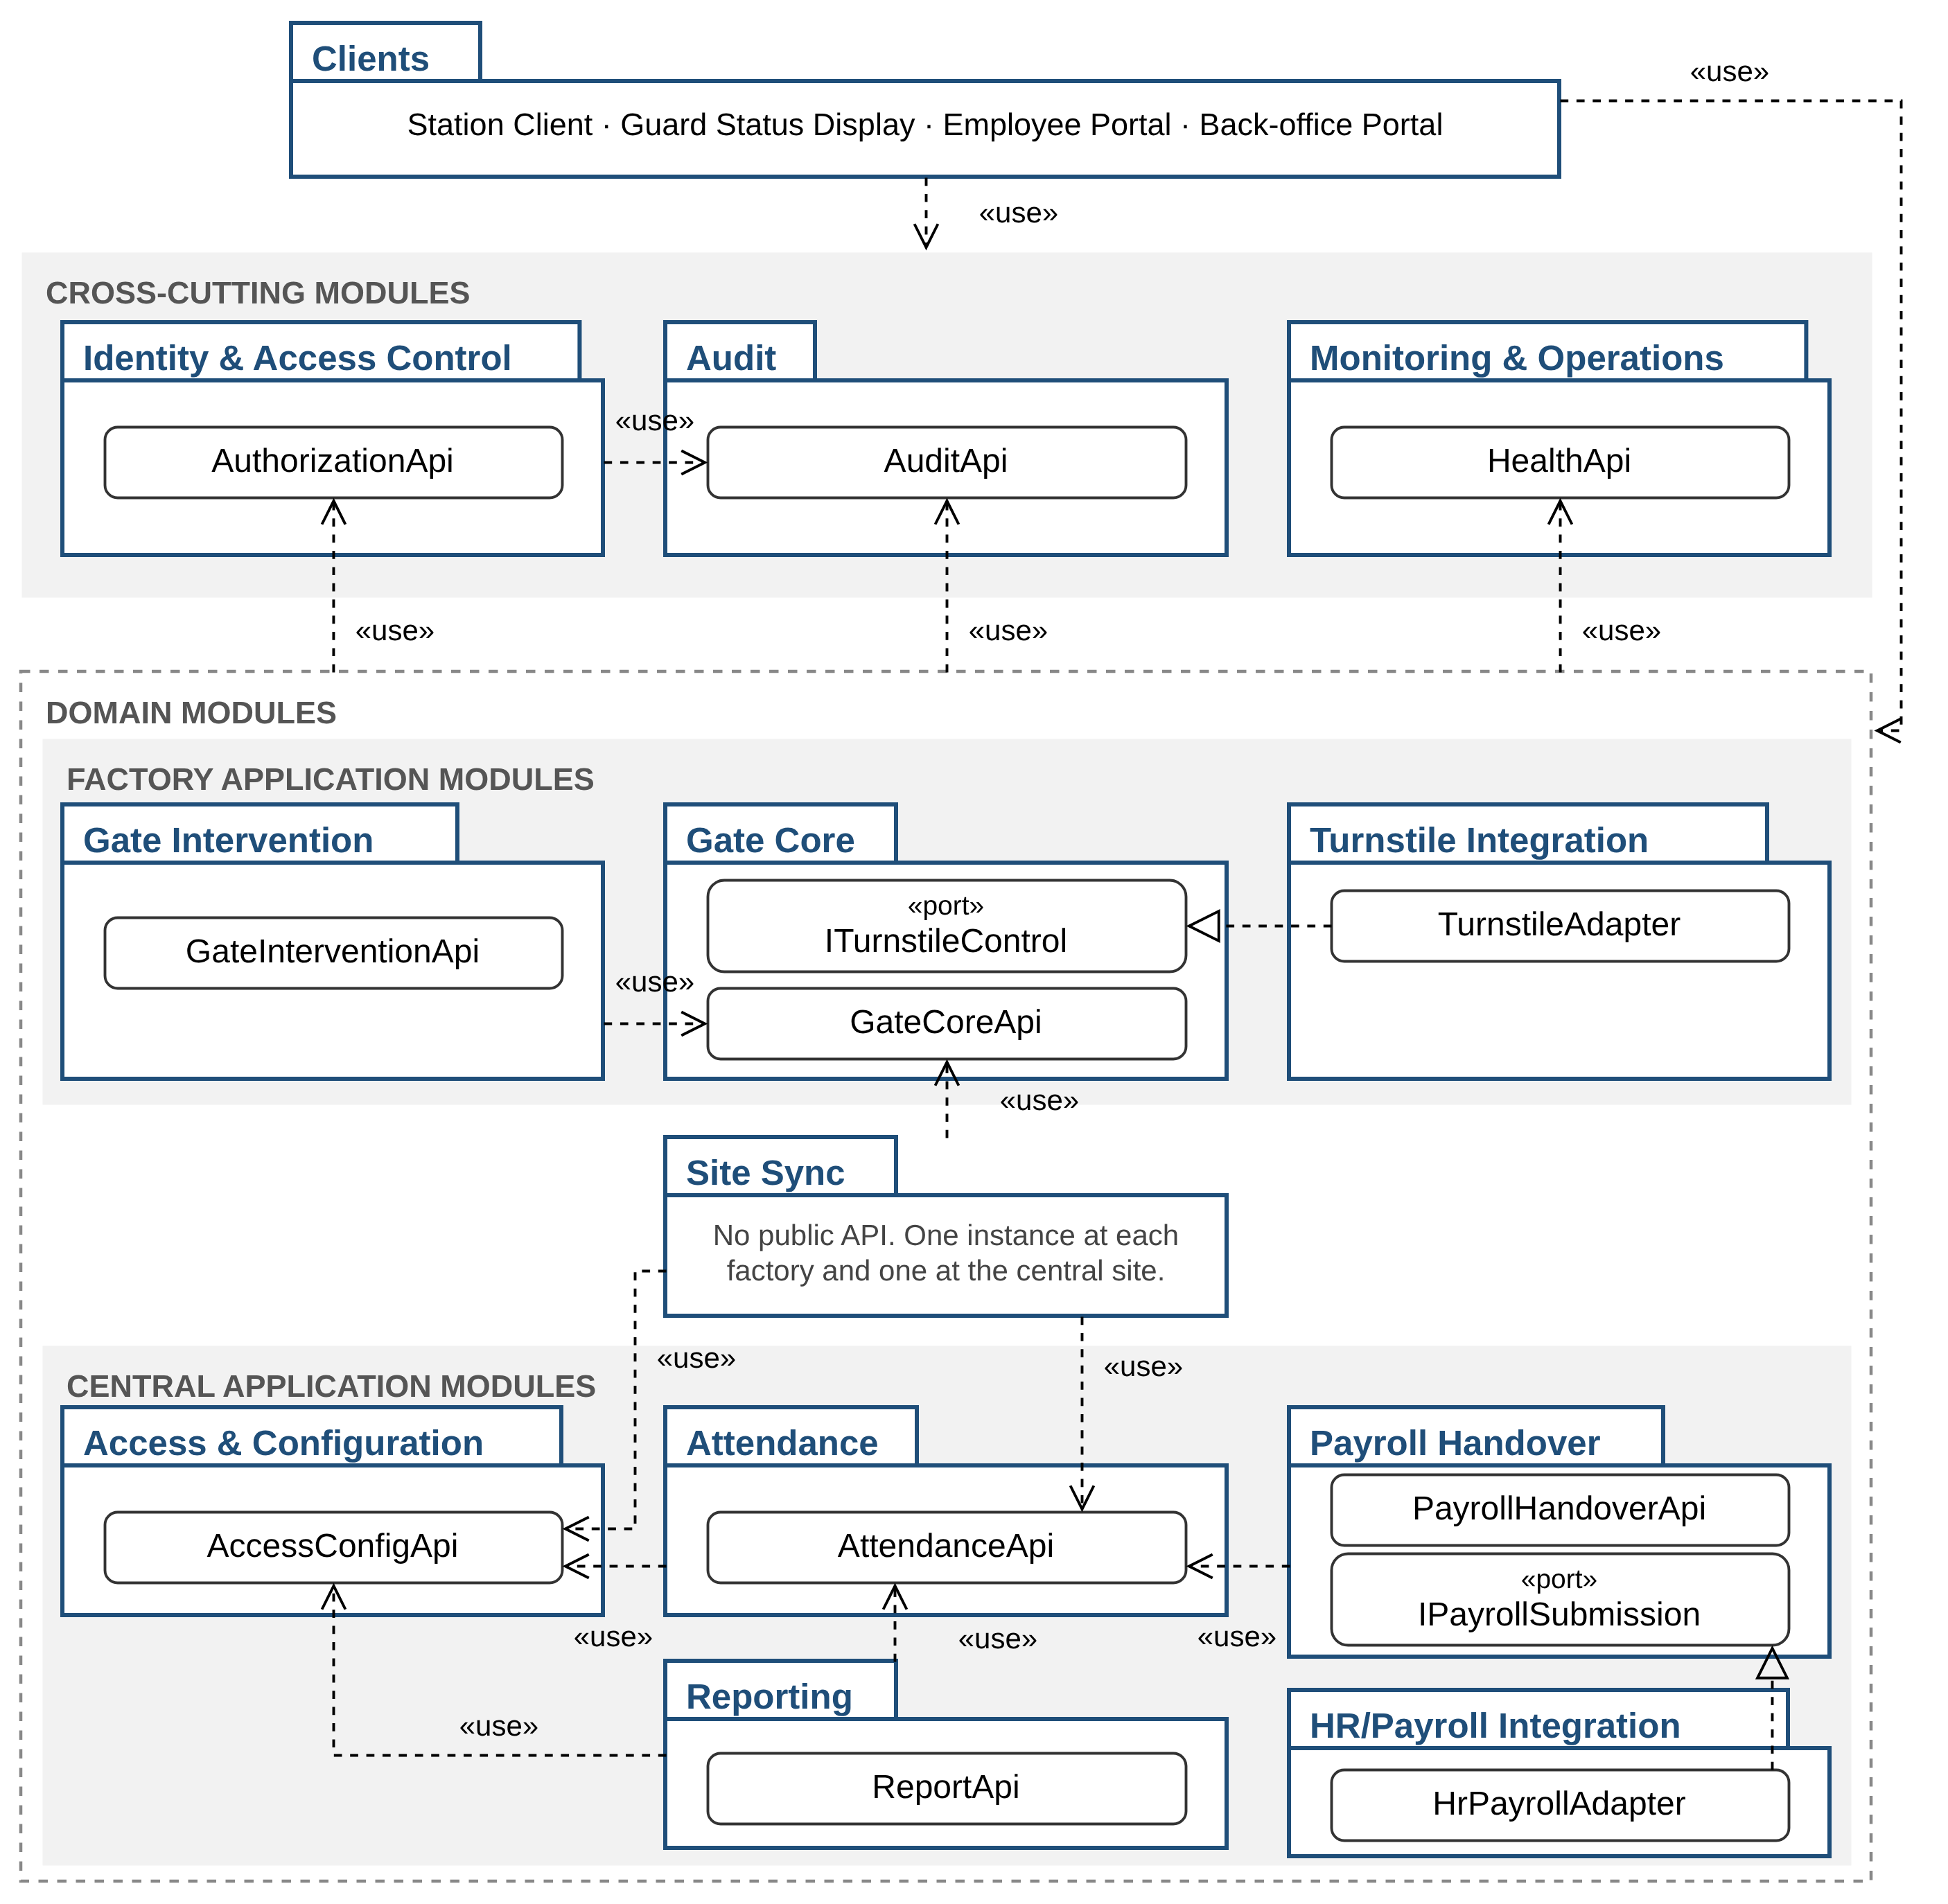
\includegraphics[width=450.0pt,height=463.5pt,keepaspectratio]{diagram/module-view/figure-4-1-module-view.png}

\end{center}

\begin{center}

\textbf{Figure 4.1. Module View of the TMC System}
\phantomsection\addcontentsline{lof}{figure}{\protect\numberline{4.1}Module View of the TMC System}

\end{center}

\Needspace{6\baselineskip}
Dashed open arrows labelled \guillemotleft use\guillemotright{} show dependencies on public interfaces, not runtime message direction. Dashed arrows with hollow triangles point from adapters to the integration interfaces marked \guillemotleft port\guillemotright{} that they realize. Arrows attached to group boundaries summarize selected dependencies, not dependencies of every module in the group. Table 4.4 lists the exact module pairs.



\begin{longtable}{|>{\raggedright\arraybackslash}p{73.5pt}|>{\raggedright\arraybackslash}p{129.5pt}|>{\raggedright\arraybackslash}p{206.5pt}|}
\hline
\multicolumn{1}{|>{\columncolor{tableheader}\centering\arraybackslash}p{73.5pt}|}{\textbf{Module}} & \multicolumn{1}{>{\columncolor{tableheader}\centering\arraybackslash}p{129.5pt}|}{\textbf{Component}} & \multicolumn{1}{>{\columncolor{tableheader}\centering\arraybackslash}p{206.5pt}|}{\textbf{Responsibility}} \\
\hline
\endhead
\multicolumn{3}{c}{\rule{0pt}{20pt}\normalsize\textbf{Table 4.3. Modules and Responsibilities after Restructuring}} \\
\endlastfoot
M1 Gate Core & Gate Transaction Processor; Access Decision; Eligibility Snapshot & Coordinate and store scan states; validate QR codes, permissions, and configuration; manage versioned decision-support data. \\
\hline
M2 Turnstile Integration & Turnstile Adapter & Implement the gate control port and translate commands and outcomes according to the Controller API. \\
\hline
M3 Gate Intervention & Gate Intervention & Receive assistance records, authorize assisted and emergency actions, and request Gate Core to store cases and coordinate gate commands. \\
\hline
M4 Access \& Configuration & Access Rights Management; QR Credential Issuance; Email Link Sender; Gate Station Management; Work Schedule Policy & Manage employees, permissions, QR issuance and email display links, station/lane configuration, shift schedules, and aggregation rules. \\
\hline
M5 Attendance & Attendance Consolidation; Attendance Review & Consolidate transactions and apply approved decisions; manage discrepancy reports, assistance cases, reconciliation, and application progress. \\
\hline
M6 Reporting & Reporting & Provide queries, reports, and audit queries within authorized scopes. \\
\hline
M7 Payroll Handover & Payroll Handover & Manage periods, batch content, acknowledgements, errors, and supplementary handovers. \\
\hline
M8 HR/Payroll Integration & HR/Payroll Adapter & Translate data and responses between Payroll Handover and HR/Payroll. \\
\hline
M9 Site Sync & Site Sync & Transfer events and data changes with at-least-once delivery; track progress and processing acknowledgements. \\
\hline
M10 Identity \& Access Control & Identity \& RBAC & Authenticate users and manage sessions, accounts, roles, and permission scopes. \\
\hline
M11 Audit & Audit Log & Receive and store audit records and provide queries through a controlled access path. \\
\hline
M12 Monitoring \& Operations & Monitoring & Monitor operational status, faults, latency, and task progress, and raise alerts. One logical module with a central deployment and a deployment at each factory. \\*
\hline\noalign{\nobreak}
M13 Clients & Station Client; Guard Status Display; Employee Portal; Back-office Portal & Provide station, guard-post status, employee, and management interfaces according to role. \\
\hline
\end{longtable}
\phantomsection\addcontentsline{lot}{table}{\protect\numberline{4.3}Modules and Responsibilities after Restructuring}


\begin{itemize}[leftmargin=36pt, itemsep=2pt, topsep=4pt, parsep=2pt]
  \item \textbf{Responsibility boundaries.} In the automatic QR flow, Gate Transaction Processor creates transactions. For assistance and reconciliation, Attendance Review stores the decision, Attendance Consolidation applies it to attendance, and Gate Core updates the scan. Gate Core defines the turnstile command ports and IPassageEvents. Turnstile Adapter implements the command ports and calls IPassageEvents to report passage and lane-clear events. Payroll Handover defines IPayrollSubmission, implemented by HR/Payroll Adapter.
  \item \textbf{Inside each module.} Data-owning business modules use three layers: an entry layer (API controller, event handler, or scheduled trigger), a business layer whose facade implements the module's public interface, and a persistence layer with its repositories and the ports it defines. Gate Intervention and Reporting own no business data, so they have no persistence layer and call the owning module's interface instead. Audit and Monitoring receive calls directly at their facade and have no separate entry layer. Site Sync uses background workers and exposes no public facade. Adapters and clients keep their own simpler structure. Other modules call only the facade, never the services or repositories behind it.
\end{itemize}

\Needspace{9\baselineskip}
\subsubsection*{4.1.3. Module Dependencies}

\phantomsection
\addcontentsline{toc}{subsubsection}{4.1.3. Module Dependencies}


Table 4.4 shows which modules each module depends on and the reason for each dependency.

\begin{longtable}{|>{\raggedright\arraybackslash}p{45.5pt}|>{\raggedright\arraybackslash}p{100.5pt}|>{\raggedright\arraybackslash}p{263.5pt}|}
\hline
\multicolumn{1}{|>{\columncolor{tableheader}\centering\arraybackslash}p{45.5pt}|}{\textbf{Module}} & \multicolumn{1}{>{\columncolor{tableheader}\centering\arraybackslash}p{100.5pt}|}{\textbf{Depends On}} & \multicolumn{1}{>{\columncolor{tableheader}\centering\arraybackslash}p{263.5pt}|}{\textbf{Purpose}} \\
\hline
\endhead
\multicolumn{3}{c}{\rule{0pt}{20pt}\normalsize\textbf{Table 4.4. Module Dependencies}} \\
\endlastfoot
M1 & M11, M12 & Transfer audit and operational information. \\
\hline
M2 & M1, M12 & Implement the turnstile command ports defined by Gate Core, pass PASSAGE and LANE\_CLEAR to Gate Core through IPassageEvents, and report integration status. \\
\hline
M3 & M1, M10, M11 & Record cases, use the control port, check authorization, and record audit evidence. \\
\hline
M4 & M10, M11 & Check authorization and record change histories. \\
\hline
M5 & M4, M10, M11 & Use aggregation rules, check authorization, and record audit evidence. \\
\hline
M6 & M4, M5, M10, M11 & Obtain rules and attendance data, check scope, and query audit records. \\
\hline
M7 & M5, M10, M11, M12 & Obtain period data and cases, check authorization, record audit evidence, and raise alerts. \\
\hline
M8 & M7 & Implement IPayrollSubmission. \\
\hline
M9 & M1, M4, M5, M11, M12 & Use data exchange contracts, record evidence, and monitor synchronization. \\
\hline
M10 & M11 & Record authentication and permission change evidence. \\
\hline
M11 & No business module dependencies & Receive and provide audit data. \\
\hline
M12 & No business module dependencies & Receive operational information. \\*
\hline\noalign{\nobreak}
M13 & M1, M3, M4, M5, M6, M7, M10, M12 & Access functions through public interfaces. \\
\hline
\end{longtable}
\phantomsection\addcontentsline{lot}{table}{\protect\numberline{4.4}Module Dependencies}


For example, Gate Transaction Processor calls Turnstile Adapter at runtime, but in the contract graph Turnstile Integration depends on the port defined by Gate Core.

\Needspace{6\baselineskip}
The modules follow these dependency rules:

\begin{itemize}[leftmargin=36pt, itemsep=2pt, topsep=4pt, parsep=2pt]

  \item Other modules are reached only through their public interfaces, never through their internal components or data.

  \item Only the data owner updates its data; others send requests through its interface.

  \item The dependencies in Table 4.4 have no cycles.

  \item Reporting checks authorization through Identity \& RBAC before querying Audit Log, and Audit Log never calls back, which avoids a cycle.

  \item Gate Core and Turnstile Integration do not depend on Reporting, Payroll Handover, HR/Payroll Integration, or Attendance, so the kiosk does not wait for these modules. Interference through shared resources still needs limits and performance tests.

\end{itemize}

\Needspace{9\baselineskip}
\subsubsection*{4.1.4. FR Coverage after Restructuring}

\phantomsection
\addcontentsline{toc}{subsubsection}{4.1.4. FR Coverage after Restructuring}


Table 4.5 gives the main and supporting components for each of the 26 functional requirements.

\begin{longtable}{|>{\raggedright\arraybackslash}p{41.5pt}|>{\raggedright\arraybackslash}p{187.5pt}|>{\raggedright\arraybackslash}p{179.5pt}|}
\hline
\multicolumn{1}{|>{\columncolor{tableheader}\centering\arraybackslash}p{41.5pt}|}{\textbf{FR}} & \multicolumn{1}{>{\columncolor{tableheader}\centering\arraybackslash}p{187.5pt}|}{\textbf{Primarily Responsible Components}} & \multicolumn{1}{>{\columncolor{tableheader}\centering\arraybackslash}p{179.5pt}|}{\textbf{Collaborating Components}} \\
\hline
\endhead
\multicolumn{3}{c}{\rule{0pt}{20pt}\normalsize\textbf{Table 4.5. FR-to-Component Mapping after Restructuring}} \\
\endlastfoot
FR-01.1 & Access Rights Management & Identity \& RBAC; Back-office Portal \\
\hline
FR-01.2 & QR Credential Issuance; Access Decision & Eligibility Snapshot \\
\hline
FR-01.3 & QR Credential Issuance; Email Link Sender & Employee Portal; Identity \& RBAC; TMC email service \\
\hline
FR-01.4 & Access Rights Management & Site Sync; Eligibility Snapshot; Identity \& RBAC \\
\hline
FR-02.1 & Gate Station Management & Site Sync; Eligibility Snapshot \\
\hline
FR-02.2 & Gate Transaction Processor; Turnstile Adapter & --- \\
\hline
FR-02.3 & Monitoring & Station Client; Turnstile Adapter; Gate Transaction Processor \\
\hline
FR-02.4 & Gate Intervention & Identity \& RBAC; Gate Transaction Processor; Turnstile Adapter; Audit Log \\
\hline
FR-03.1 & Station Client; Gate Transaction Processor & Access Decision \\
\hline
FR-03.2 & Access Decision & Eligibility Snapshot; Access Rights Management \\
\hline
FR-03.3 & Gate Transaction Processor; Attendance Consolidation & Turnstile Adapter; Site Sync; Attendance Review \\
\hline
FR-03.4 & Gate Transaction Processor; Attendance Consolidation & Station Client; Site Sync \\
\hline
FR-03.5 & Gate Transaction Processor; Attendance Consolidation & Gate Station Management; Eligibility Snapshot \\
\hline
FR-03.6 & Gate Transaction Processor & Site Sync; Attendance Review; Audit Log \\
\hline
FR-04.1 & Reporting & Attendance Consolidation; Identity \& RBAC \\
\hline
FR-04.2 & Reporting & Attendance Consolidation; Work Schedule Policy \\
\hline
FR-04.3 & Payroll Handover; HR/Payroll Adapter & Attendance Consolidation; Attendance Review; Monitoring \\
\hline
FR-04.4 & Attendance Review; Attendance Consolidation & Employee Portal; Back-office Portal; Identity \& RBAC; Audit Log \\
\hline
FR-04.5 & Audit Log & Components originating business and administrative actions \\
\hline
FR-04.6 & Reporting & Attendance Consolidation; Identity \& RBAC; Employee Portal; Back-office Portal \\
\hline
FR-04.7 & Reporting; Audit Log & Identity \& RBAC \\
\hline
FR-05.1 & Identity \& RBAC & Back-office Portal; Audit Log \\
\hline
FR-05.2 & Work Schedule Policy & Back-office Portal; Identity \& RBAC \\
\hline
FR-05.3 & Monitoring & Station Client; Turnstile Adapter; Gate Transaction Processor; Site Sync; Payroll Handover \\
\hline
FR-05.4 & Monitoring and operational mechanisms of data-owning components & Data-owning modules \\*
\hline\noalign{\nobreak}
FR-05.5 & Identity \& RBAC & Employee Portal; Back-office Portal; Audit Log \\
\hline
\end{longtable}
\phantomsection\addcontentsline{lot}{table}{\protect\numberline{4.5}FR-to-Component Mapping after Restructuring}


\Needspace{9\baselineskip}
\subsubsection*{4.1.5. Driving Characteristic Coverage}

\phantomsection
\addcontentsline{toc}{subsubsection}{4.1.5. Driving Characteristic Coverage}


Table 4.6 shows which design mechanisms support each driving characteristic.

\begin{longtable}{|>{\raggedright\arraybackslash}p{92.5pt}|>{\raggedright\arraybackslash}p{82.5pt}|>{\raggedright\arraybackslash}p{234.5pt}|}
\hline
\multicolumn{1}{|>{\columncolor{tableheader}\centering\arraybackslash}p{92.5pt}|}{\textbf{Characteristic}} & \multicolumn{1}{>{\columncolor{tableheader}\centering\arraybackslash}p{82.5pt}|}{\textbf{Related Requirements}} & \multicolumn{1}{>{\columncolor{tableheader}\centering\arraybackslash}p{234.5pt}|}{\textbf{Design Mechanism}} \\
\hline
\endhead
\multicolumn{3}{c}{\rule{0pt}{20pt}\normalsize\textbf{Table 4.6. Driving Characteristics Covered by the Logical Design}} \\
\endlastfoot
AC-01 Reliability/Data Integrity & NFR-02; FR-03.3--FR-03.6; I-03 & Gate Transaction Processor owns durable recording and scan states; Attendance Consolidation blocks duplicates; undetermined outcomes are kept for inquiry. \\
\hline
AC-02 Availability & FR-02.3; FR-05.3 & Monitoring detects outages; components recover from stored states and events. Local access data may be used only for a limited time (I-10). \\
\hline
AC-03 Performance & NFR-01; IC-02 & Only Gate Transaction Processor, Access Decision, Eligibility Snapshot, and Turnstile Adapter sit on the kiosk path; reporting and handover do not. \\
\hline
AC-04 Security/Privacy & NFR-03; NFR-04; FR-01.2; FR-03.2; FR-05.5; I-04 & Identity \& RBAC controls actions and data scope; QR codes and screens show minimal personal data; HR approves assistance cases. \\
\hline
AC-05 Auditability & NFR-03; FR-04.4; FR-04.5; FR-04.7; I-04 & Evidence is stored at its source and sent to Audit Log; cases, decisions, and handovers are linked; audit queries are authorized first. \\*
\hline\noalign{\nobreak}
AC-06 Interoperability & FR-02.2; FR-04.3; IC-01; IC-02; I-01--I-03; I-05; I-07 & Two ports and adapters isolate the external APIs and interpret their signals and acknowledgements. \\
\hline
\end{longtable}
\phantomsection\addcontentsline{lot}{table}{\protect\numberline{4.6}Driving Characteristics Covered by the Logical Design}


\Needspace{9\baselineskip}
\subsubsection*{4.1.6. Inside the Modules}

\phantomsection
\addcontentsline{toc}{subsubsection}{4.1.6. Inside the Modules}


Figures 4.2--4.14 show the inside of each module. These figures are UML-inspired module views: they show the static decomposition and the dependencies between parts, not the order of runtime messages. They use this notation:

\begin{itemize}[leftmargin=36pt, itemsep=2pt, topsep=4pt, parsep=2pt]
  \item A dashed open arrow labelled \guillemotleft use\guillemotright{} means that one part depends on another.
  \item The facade implements the module's public interface; this is drawn as a dashed arrow ending in a hollow triangle.
  \item A box marked \guillemotleft port\guillemotright{} is an integration interface that the module owns and an adapter implements; this is our own label, not a UML port.
  \item Each frame is divided into \guillemotleft layer\guillemotright{} areas (Entry, Business, Persistence) where the module has them.
  \item Dashed boxes outside a module frame are public interfaces of other modules, such as AuditApi, or external APIs and systems, such as the Controller API or the HR/Payroll API.
\end{itemize}

The component names below module level are our proposed decomposition. Table 4.3 stays the reference for module responsibilities, and Tables 4.7--4.19 under the figures only explain their components.

\textbf{Names in the figures.} Names without spaces, such as GateTransactionProcessor, refer to the same parts as their spaced names in the text; each module's figure and table show any further decomposition.

\noindent\begin{minipage}{\linewidth}
Figure 4.2 shows the inside of Gate Core, and Table 4.7 describes its components.

\vspace{6pt}
\centering
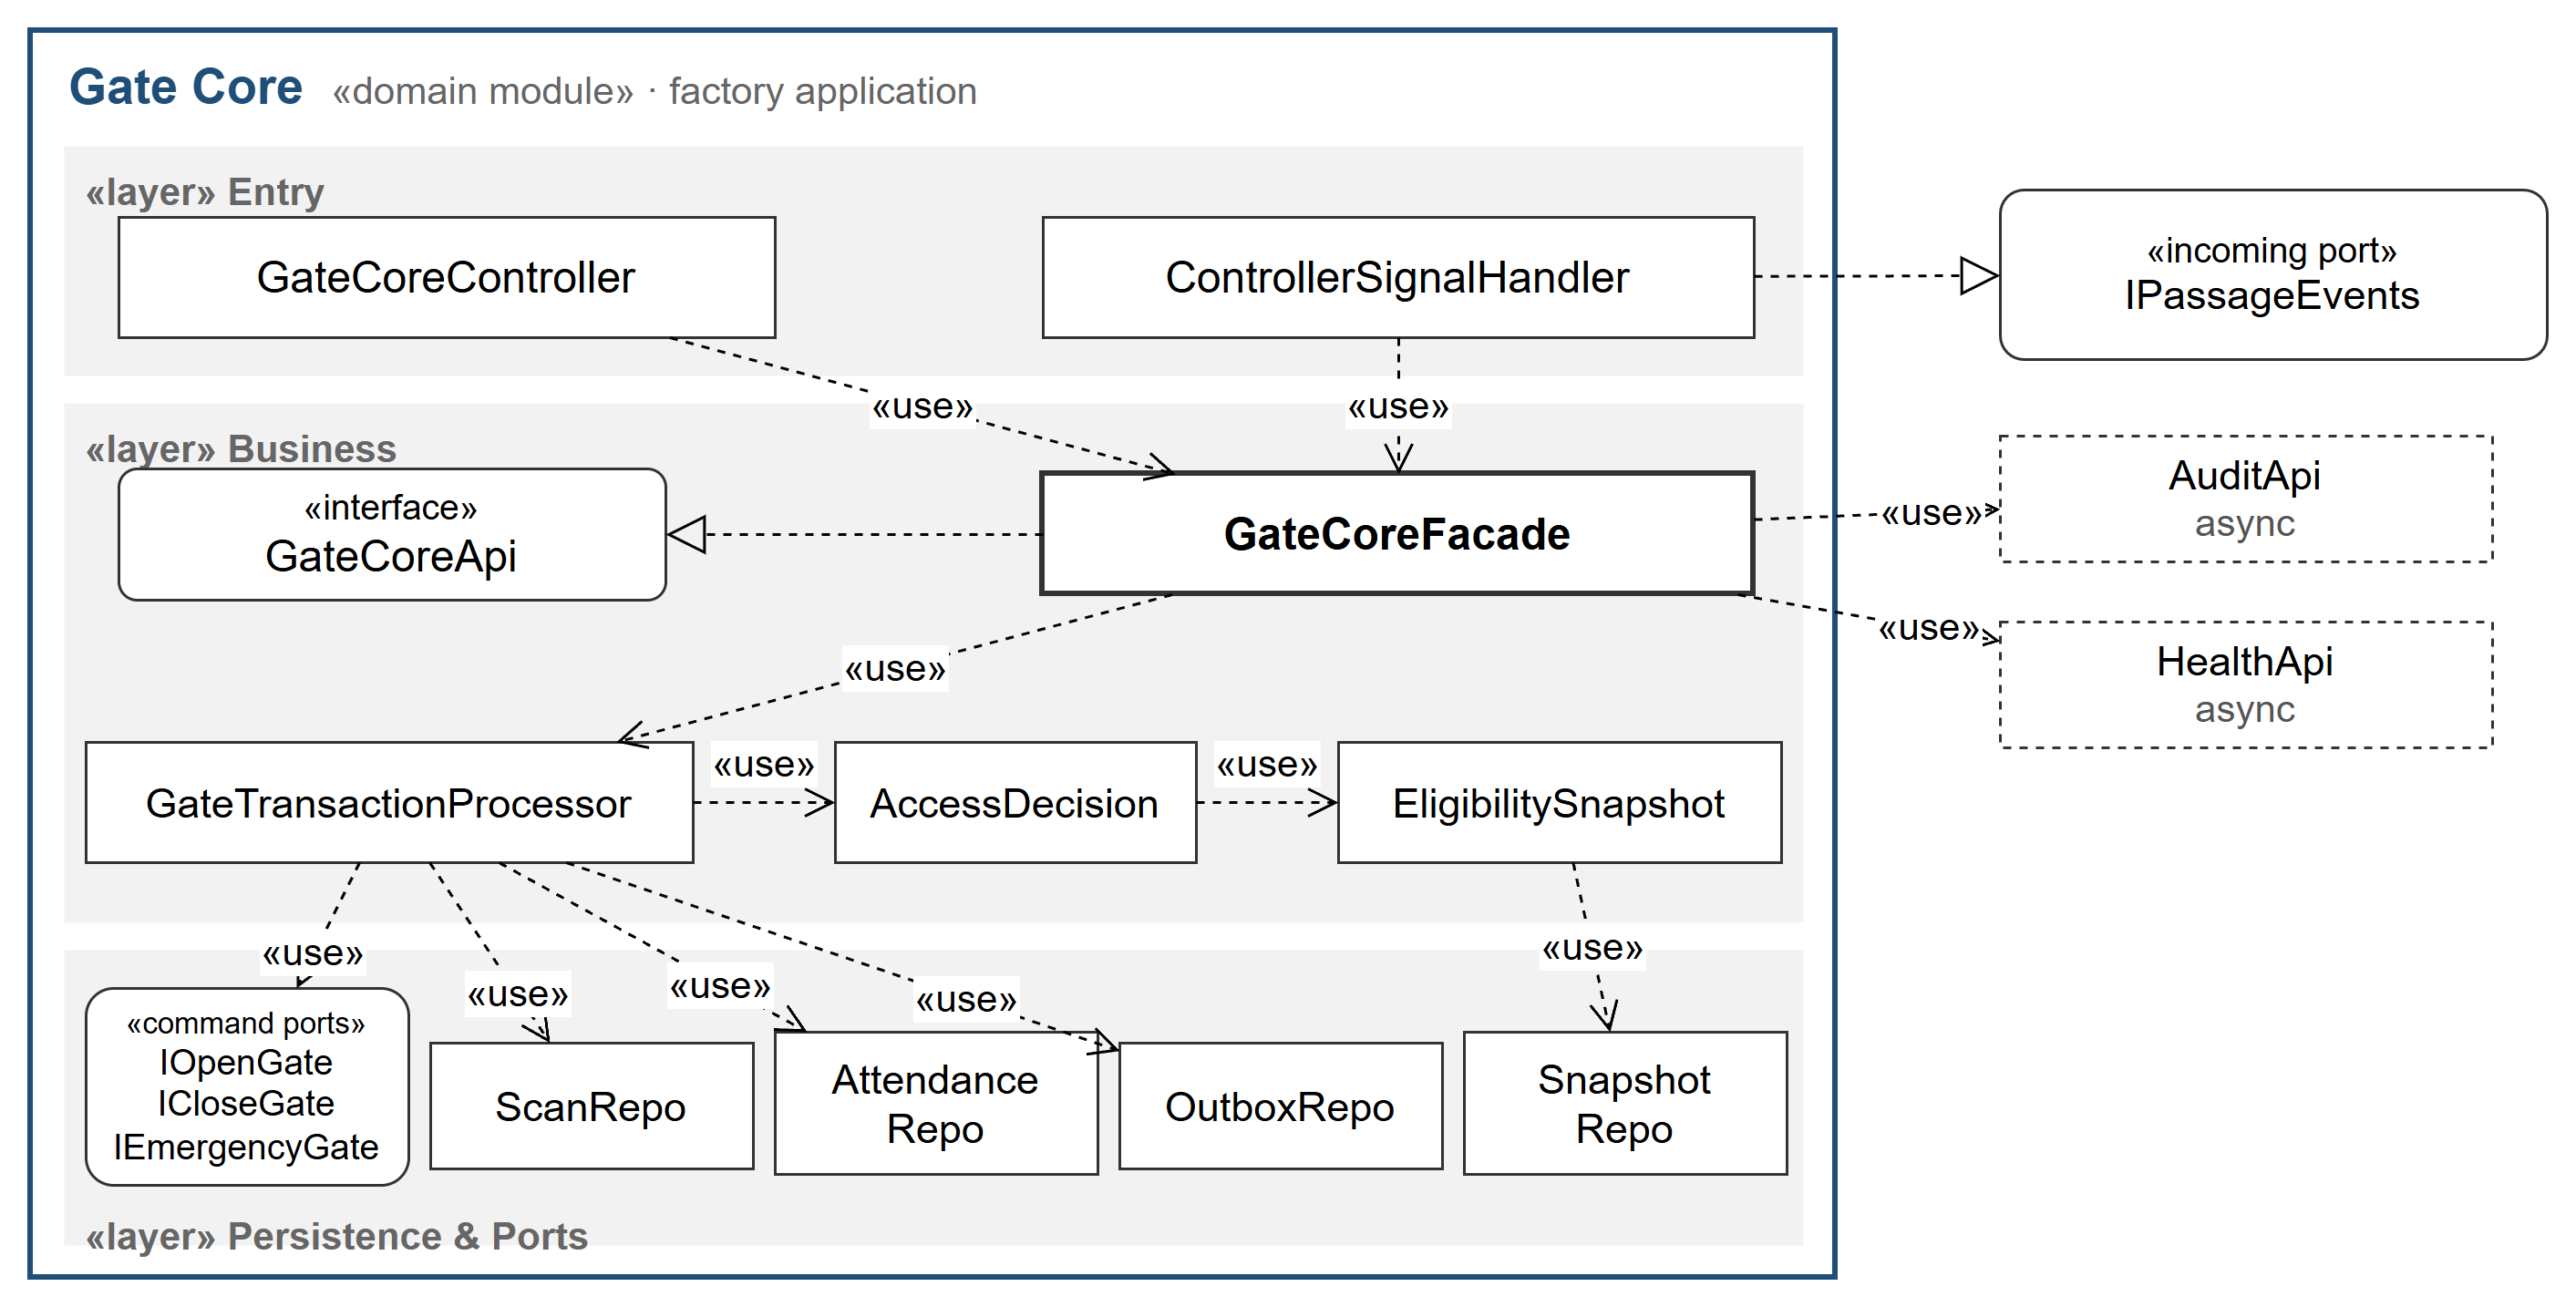
\includegraphics[width=435.8pt]{diagram/modules/figure-4-2-m1.png}

\vspace{6pt}
\textbf{Figure 4.2. M1 Gate Core}
\phantomsection\addcontentsline{lof}{figure}{\protect\numberline{4.2}M1 Gate Core}

\vspace{8pt}
{\small
\begin{tabular}{|>{\raggedright\arraybackslash}p{120pt}|>{\raggedright\arraybackslash}p{290pt}|}
\hline
\multicolumn{1}{|>{\columncolor{tableheader}\centering\arraybackslash}p{120pt}|}{\textbf{Component}} & \multicolumn{1}{>{\columncolor{tableheader}\centering\arraybackslash}p{290pt}|}{\textbf{Responsibility}} \\
\hline
GateCoreController & Receives scans from Station Client, guard actions from Gate Intervention, and access changes and resolutions from Site Sync. \\
\hline
ControllerSignalHandler & Receives PASSAGE and LANE\_CLEAR for a lane and command through IPassageEvents, which Gate Core implements and Turnstile Integration calls. OPEN\_CONFIRMED and CLOSED are not callbacks; they come back as the results of openGate and closeGate. \\
\hline
GateTransactionProcessor & Keeps scan and gate-cycle states, reserves the lane, sends controller commands, and creates attendance only after passage. \\
\hline
AccessDecision, EligibilitySnapshot & Check whether the versioned access data is usable, select normal or degraded mode (I-10), and check the QR code, permission, and configuration. Return CANNOT PROCESS when the required data cannot be used. \\
\hline
Repositories & ScanRepo and AttendanceRepo hold the original factory records. OutboxRepo stores Gate Event Feed events and audit evidence in the same transaction; audit and health data leave asynchronously, never on the scan path. \\
\hline
\end{tabular}
}

\vspace{6pt}
\textbf{Table 4.7. Components of M1 Gate Core}
\phantomsection\addcontentsline{lot}{table}{\protect\numberline{4.7}Components of M1 Gate Core}
\end{minipage}

\vspace{14pt}

\noindent\begin{minipage}{\linewidth}
Figure 4.3 shows the inside of Turnstile Integration, and Table 4.8 describes its components.

\vspace{6pt}
\centering
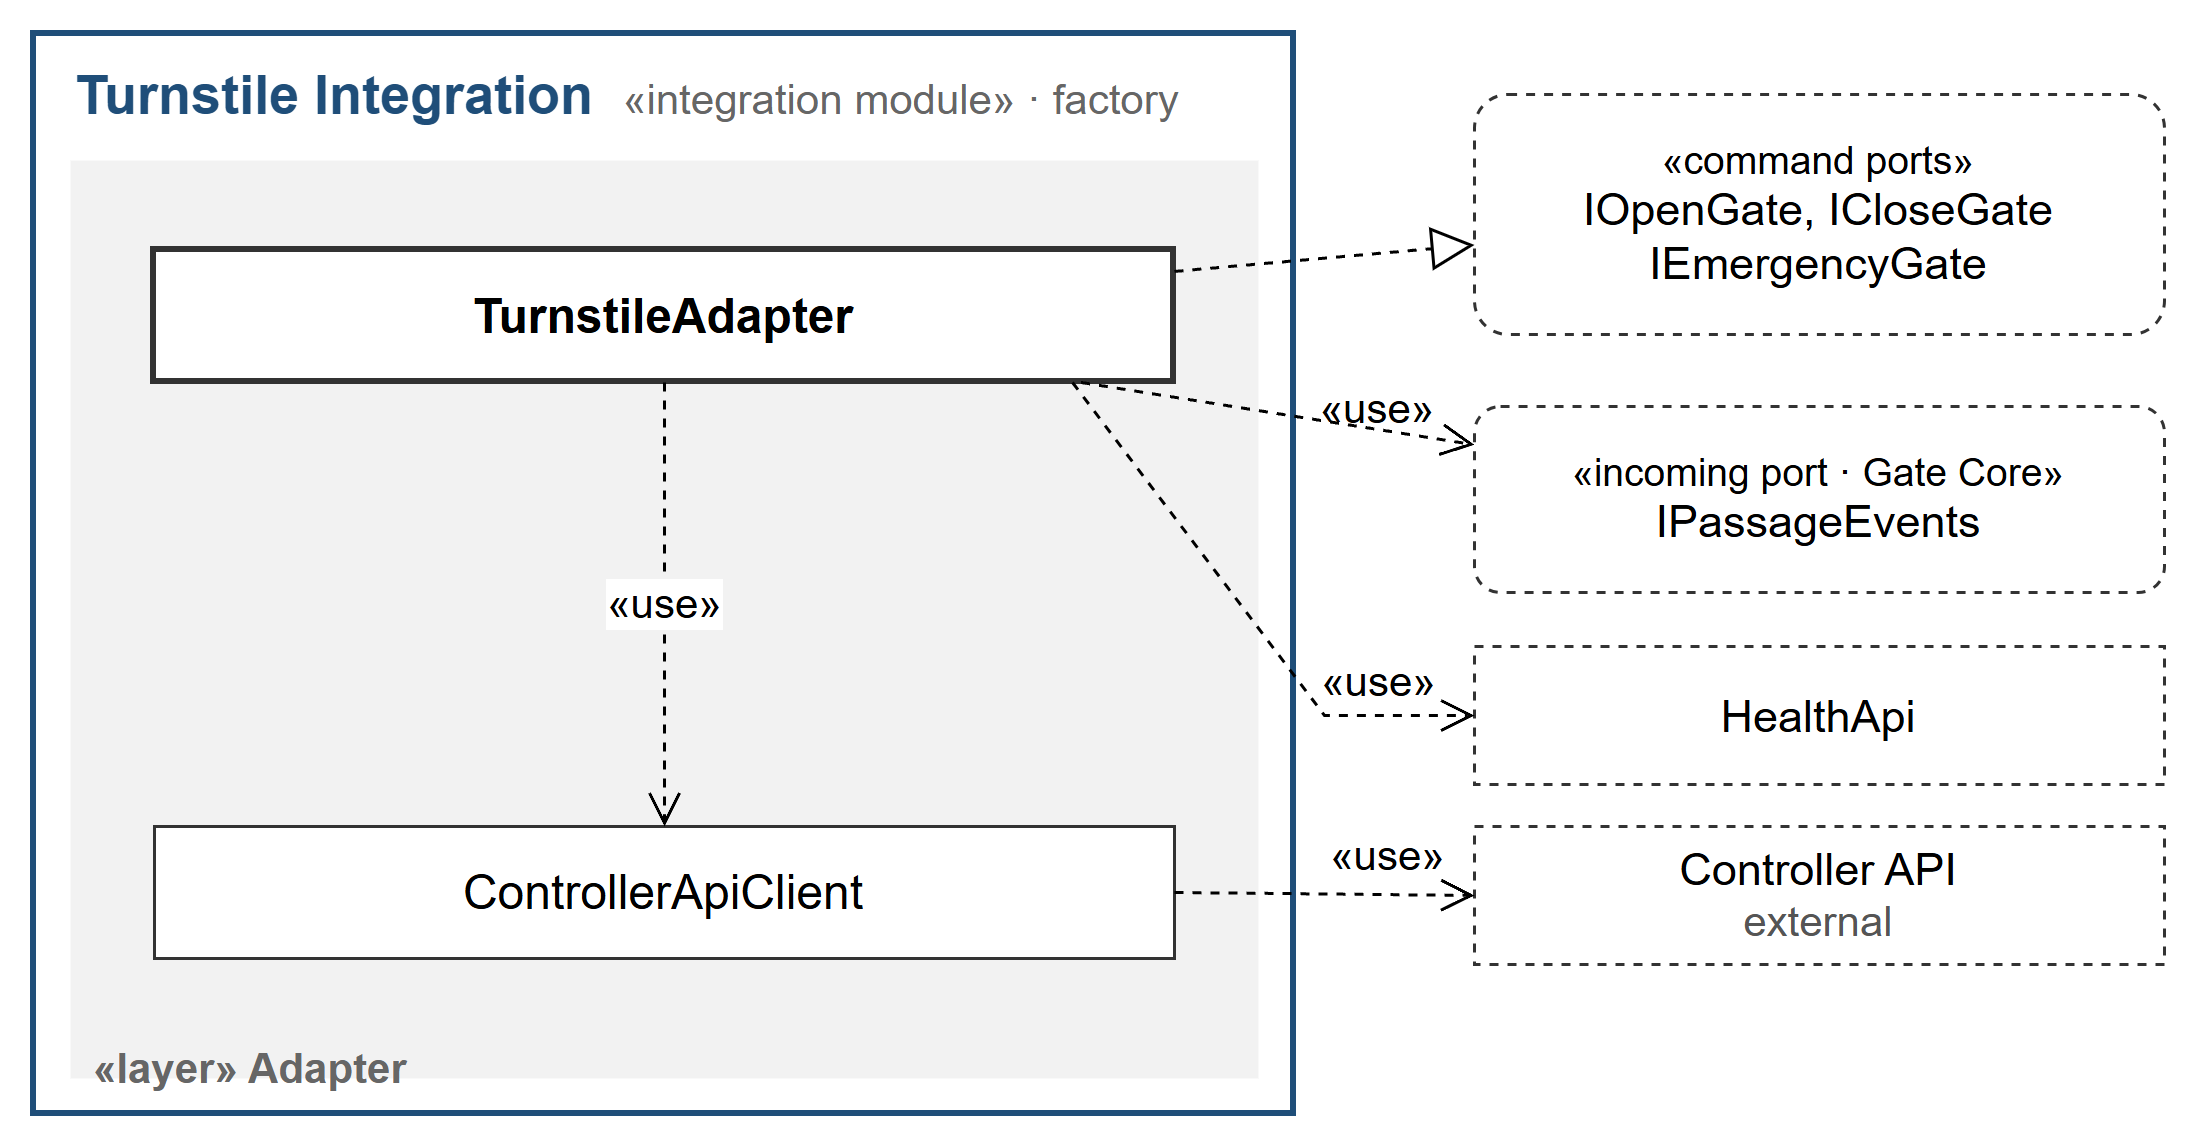
\includegraphics[width=345.6pt]{diagram/modules/figure-4-3-m2.png}

\vspace{6pt}
\textbf{Figure 4.3. M2 Turnstile Integration}
\phantomsection\addcontentsline{lof}{figure}{\protect\numberline{4.3}M2 Turnstile Integration}

\vspace{8pt}
{\small
\begin{tabular}{|>{\raggedright\arraybackslash}p{120pt}|>{\raggedright\arraybackslash}p{290pt}|}
\hline
\multicolumn{1}{|>{\columncolor{tableheader}\centering\arraybackslash}p{120pt}|}{\textbf{Component}} & \multicolumn{1}{>{\columncolor{tableheader}\centering\arraybackslash}p{290pt}|}{\textbf{Responsibility}} \\
\hline
TurnstileAdapter & Implements the command ports IOpenGate, ICloseGate, and IEmergencyGate (and the status query where the API has one), translates commands and results, and keeps ``received'', ``opened'', and ``uncertain'' apart. It forwards PASSAGE and LANE\_CLEAR to Gate Core through IPassageEvents. \\
\hline
ControllerApiClient & Calls the Controller API and receives its signals (I-01, I-05). \\
\hline
\end{tabular}
}

\vspace{6pt}
\textbf{Table 4.8. Components of M2 Turnstile Integration}
\phantomsection\addcontentsline{lot}{table}{\protect\numberline{4.8}Components of M2 Turnstile Integration}
\end{minipage}

\vspace{14pt}

\noindent\begin{minipage}{\linewidth}
Figure 4.4 shows the inside of Gate Intervention, and Table 4.9 describes its components.

\vspace{6pt}
\centering
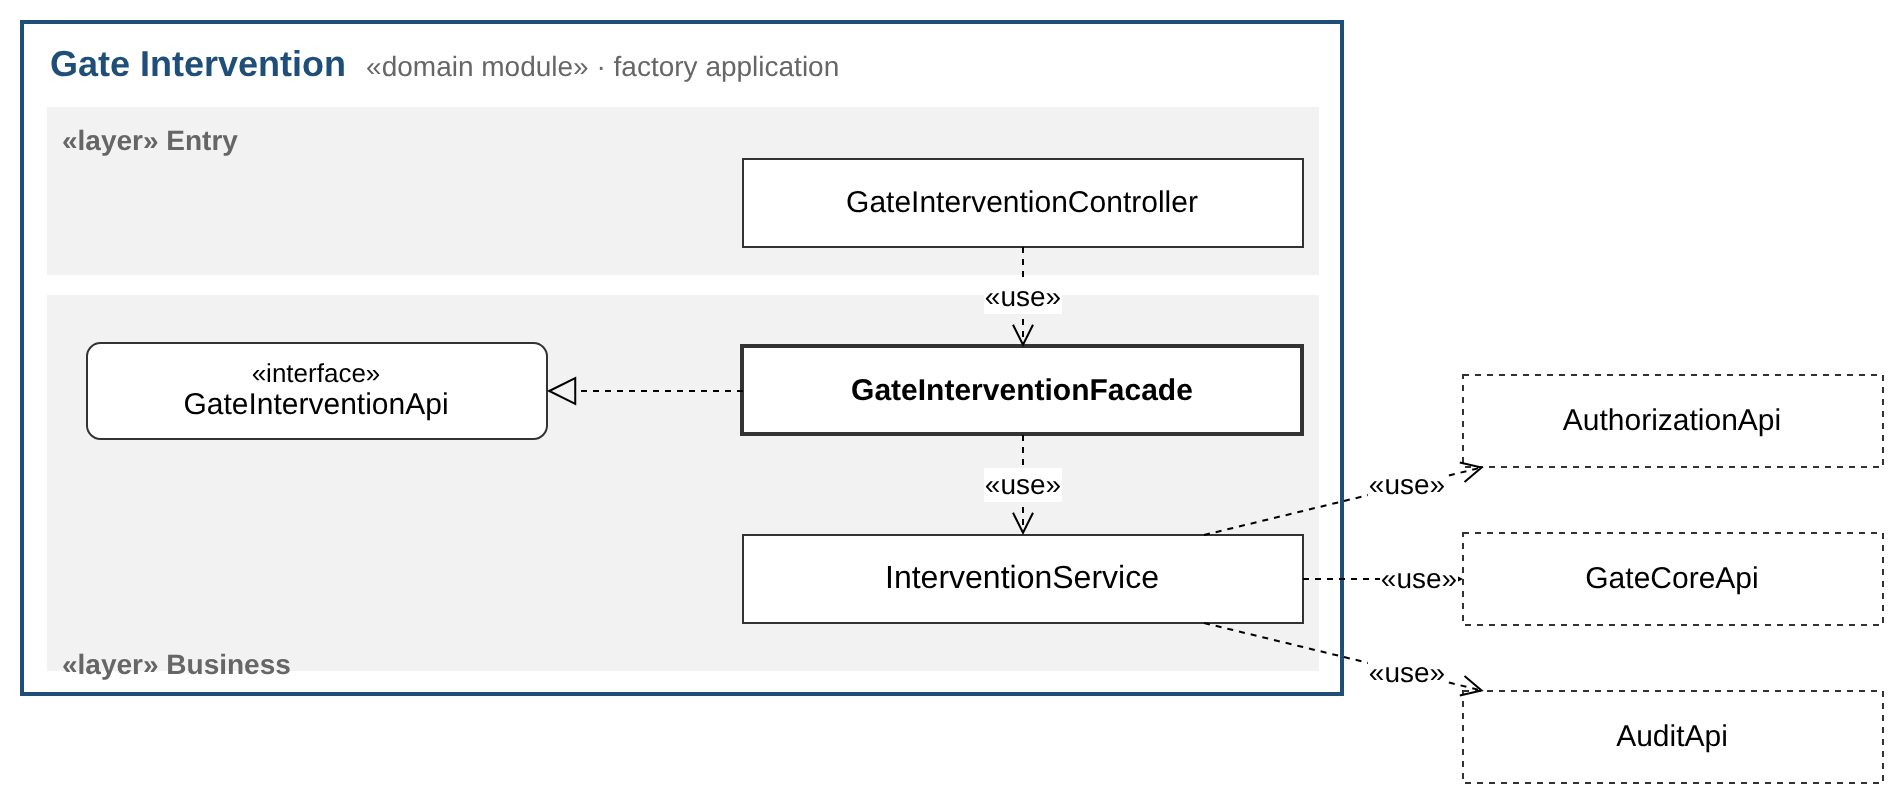
\includegraphics[width=450pt]{diagram/modules/figure-4-4-m3.png}

\vspace{6pt}
\textbf{Figure 4.4. M3 Gate Intervention}
\phantomsection\addcontentsline{lof}{figure}{\protect\numberline{4.4}M3 Gate Intervention}

\vspace{8pt}
{\small
\begin{tabular}{|>{\raggedright\arraybackslash}p{120pt}|>{\raggedright\arraybackslash}p{290pt}|}
\hline
\multicolumn{1}{|>{\columncolor{tableheader}\centering\arraybackslash}p{120pt}|}{\textbf{Component}} & \multicolumn{1}{>{\columncolor{tableheader}\centering\arraybackslash}p{290pt}|}{\textbf{Responsibility}} \\
\hline
GateInterventionController, Facade & Receive guard actions from Back-office Portal and implement GateInterventionApi. \\
\hline
InterventionService & Checks the guard's authority, assigns the supportCaseId, and asks Gate Core to store the case and open or release the gate. It owns no business data. \\
\hline
\end{tabular}
}

\vspace{6pt}
\textbf{Table 4.9. Components of M3 Gate Intervention}
\phantomsection\addcontentsline{lot}{table}{\protect\numberline{4.9}Components of M3 Gate Intervention}
\end{minipage}

\vspace{14pt}

\noindent\begin{minipage}{\linewidth}
Figure 4.5 shows the inside of Access \& Configuration, and Table 4.10 describes its components.

\vspace{6pt}
\centering
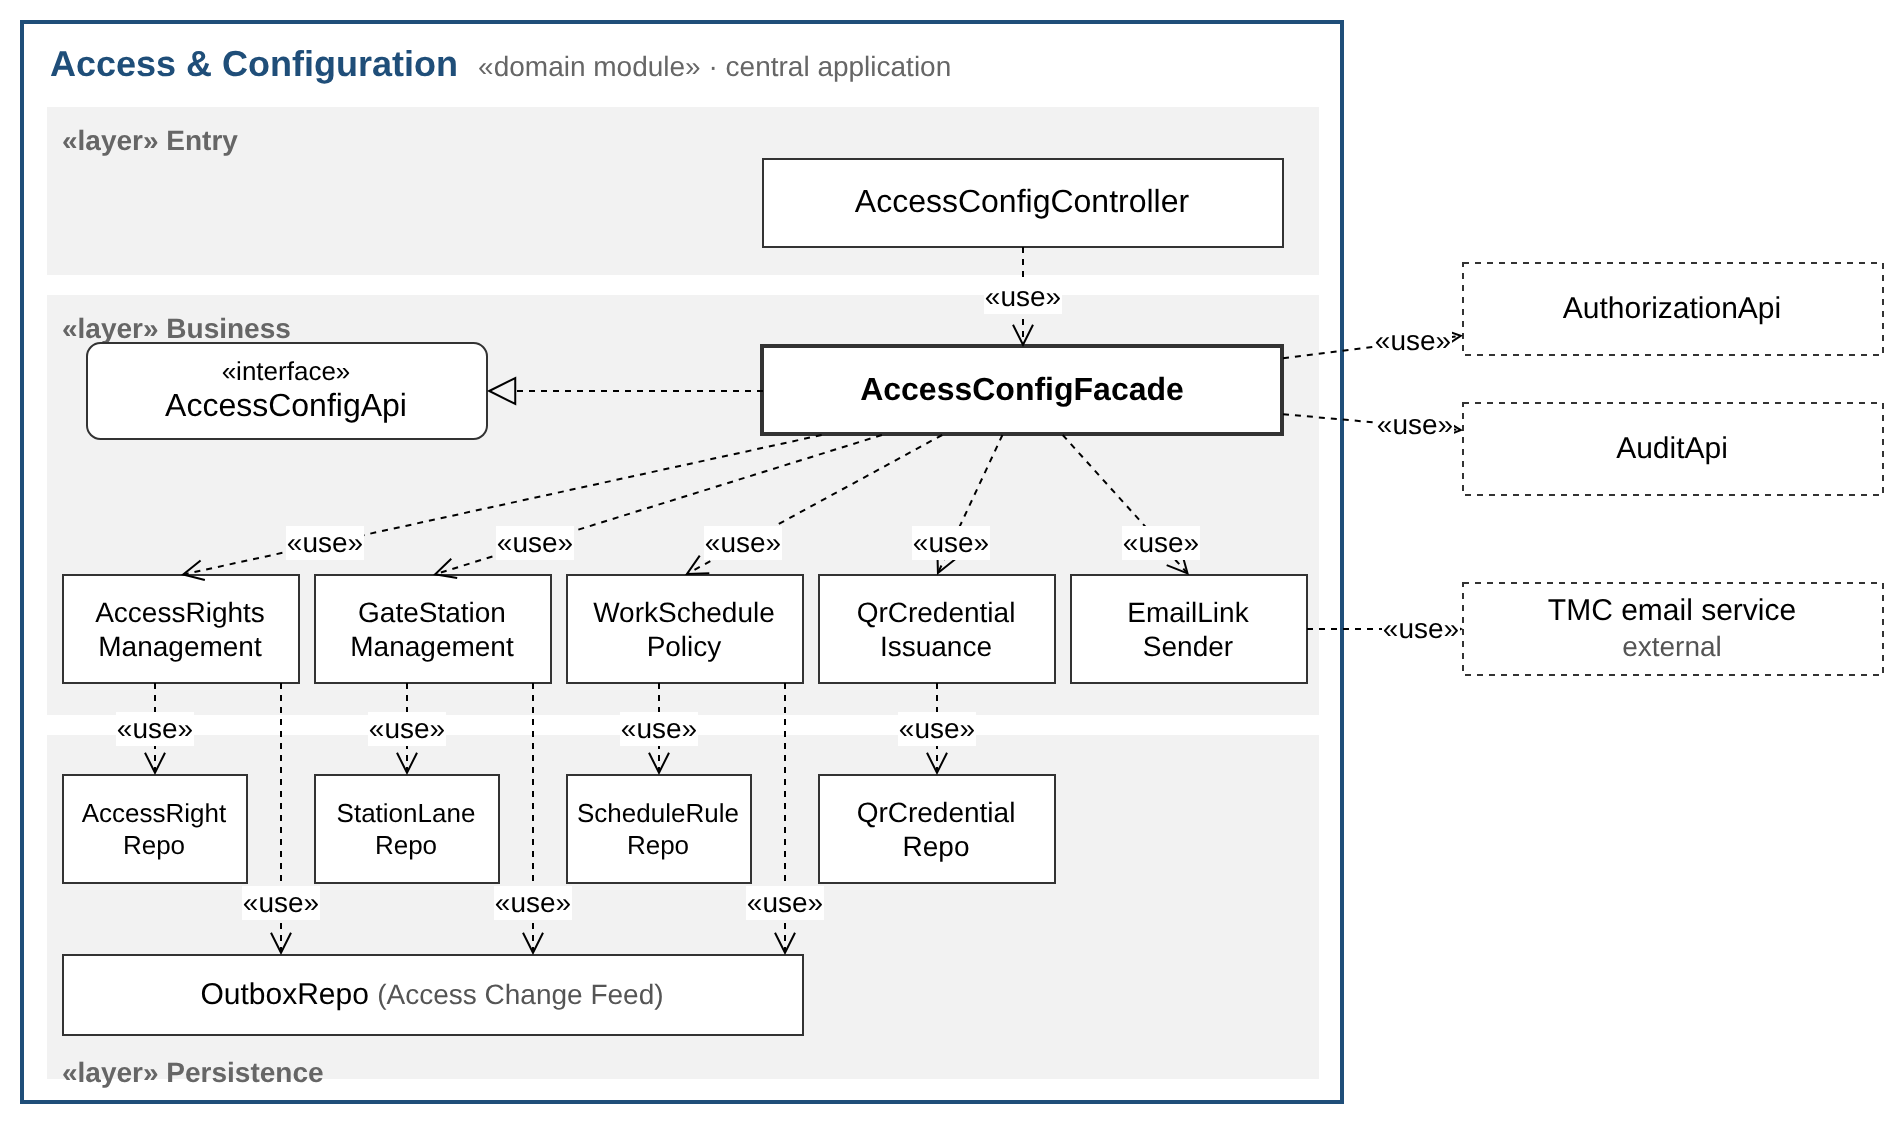
\includegraphics[width=450pt]{diagram/modules/figure-4-5-m4.png}

\vspace{6pt}
\textbf{Figure 4.5. M4 Access \& Configuration}
\phantomsection\addcontentsline{lof}{figure}{\protect\numberline{4.5}M4 Access \& Configuration}

\vspace{8pt}
{\small
\begin{tabular}{|>{\raggedright\arraybackslash}p{120pt}|>{\raggedright\arraybackslash}p{290pt}|}
\hline
\multicolumn{1}{|>{\columncolor{tableheader}\centering\arraybackslash}p{120pt}|}{\textbf{Component}} & \multicolumn{1}{>{\columncolor{tableheader}\centering\arraybackslash}p{290pt}|}{\textbf{Responsibility}} \\
\hline
AccessRightsManagement & Manages employees and their permissions. \\
\hline
QrCredentialIssuance & Issues signed, single-use QR codes that expire after 60 seconds (ADR-11). \\
\hline
GateStationManagement, WorkSchedulePolicy & Manage stations and lanes, shifts, and aggregation rules. \\
\hline
EmailLinkSender & Sends a link to the QR screen, never the QR image (I-08). \\
\hline
OutboxRepo & Stores Access Change Feed events in the same transaction as each change. \\
\hline
\end{tabular}
}

\vspace{6pt}
\textbf{Table 4.10. Components of M4 Access \& Configuration}
\phantomsection\addcontentsline{lot}{table}{\protect\numberline{4.10}Components of M4 Access \& Configuration}
\end{minipage}

\vspace{14pt}

\noindent\begin{minipage}{\linewidth}
Figure 4.6 shows the inside of Attendance, and Table 4.11 describes its components.

\vspace{6pt}
\centering
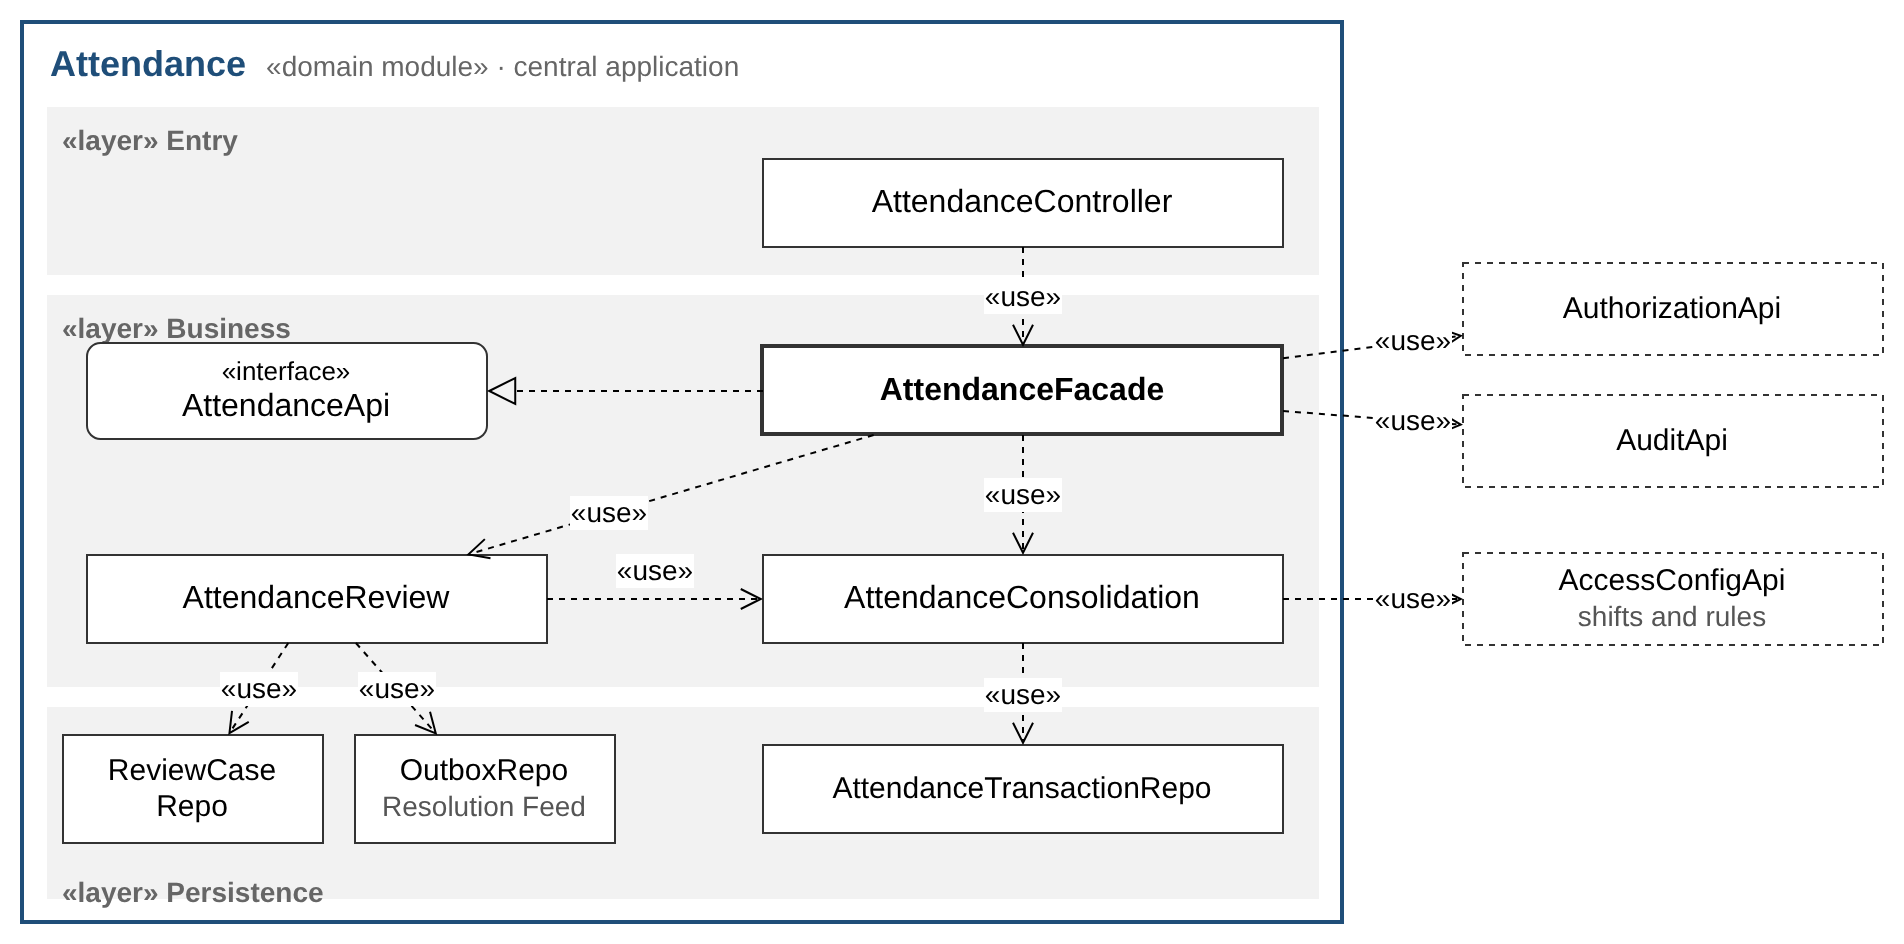
\includegraphics[width=450pt]{diagram/modules/figure-4-6-m5.png}

\vspace{6pt}
\textbf{Figure 4.6. M5 Attendance}
\phantomsection\addcontentsline{lof}{figure}{\protect\numberline{4.6}M5 Attendance}

\vspace{8pt}
{\small
\begin{tabular}{|>{\raggedright\arraybackslash}p{120pt}|>{\raggedright\arraybackslash}p{290pt}|}
\hline
\multicolumn{1}{|>{\columncolor{tableheader}\centering\arraybackslash}p{120pt}|}{\textbf{Component}} & \multicolumn{1}{>{\columncolor{tableheader}\centering\arraybackslash}p{290pt}|}{\textbf{Responsibility}} \\
\hline
AttendanceController, Facade & Implement AttendanceApi and receive Gate Event Feed events delivered by Site Sync. \\
\hline
AttendanceConsolidation & Consolidates transactions and applies approved decisions, using shifts and rules from Access \& Configuration. \\
\hline
AttendanceReview & Handles discrepancy reports, assistance cases, and reconciliation, and writes Resolution Feed events. \\
\hline
Data ownership & Attendance owns consolidated data and adjustments; the original scan records stay in Gate Core. \\
\hline
\end{tabular}
}

\vspace{6pt}
\textbf{Table 4.11. Components of M5 Attendance}
\phantomsection\addcontentsline{lot}{table}{\protect\numberline{4.11}Components of M5 Attendance}
\end{minipage}

\vspace{14pt}

\noindent\begin{minipage}{\linewidth}
Figure 4.7 shows the inside of Reporting, and Table 4.12 describes its components.

\vspace{6pt}
\centering
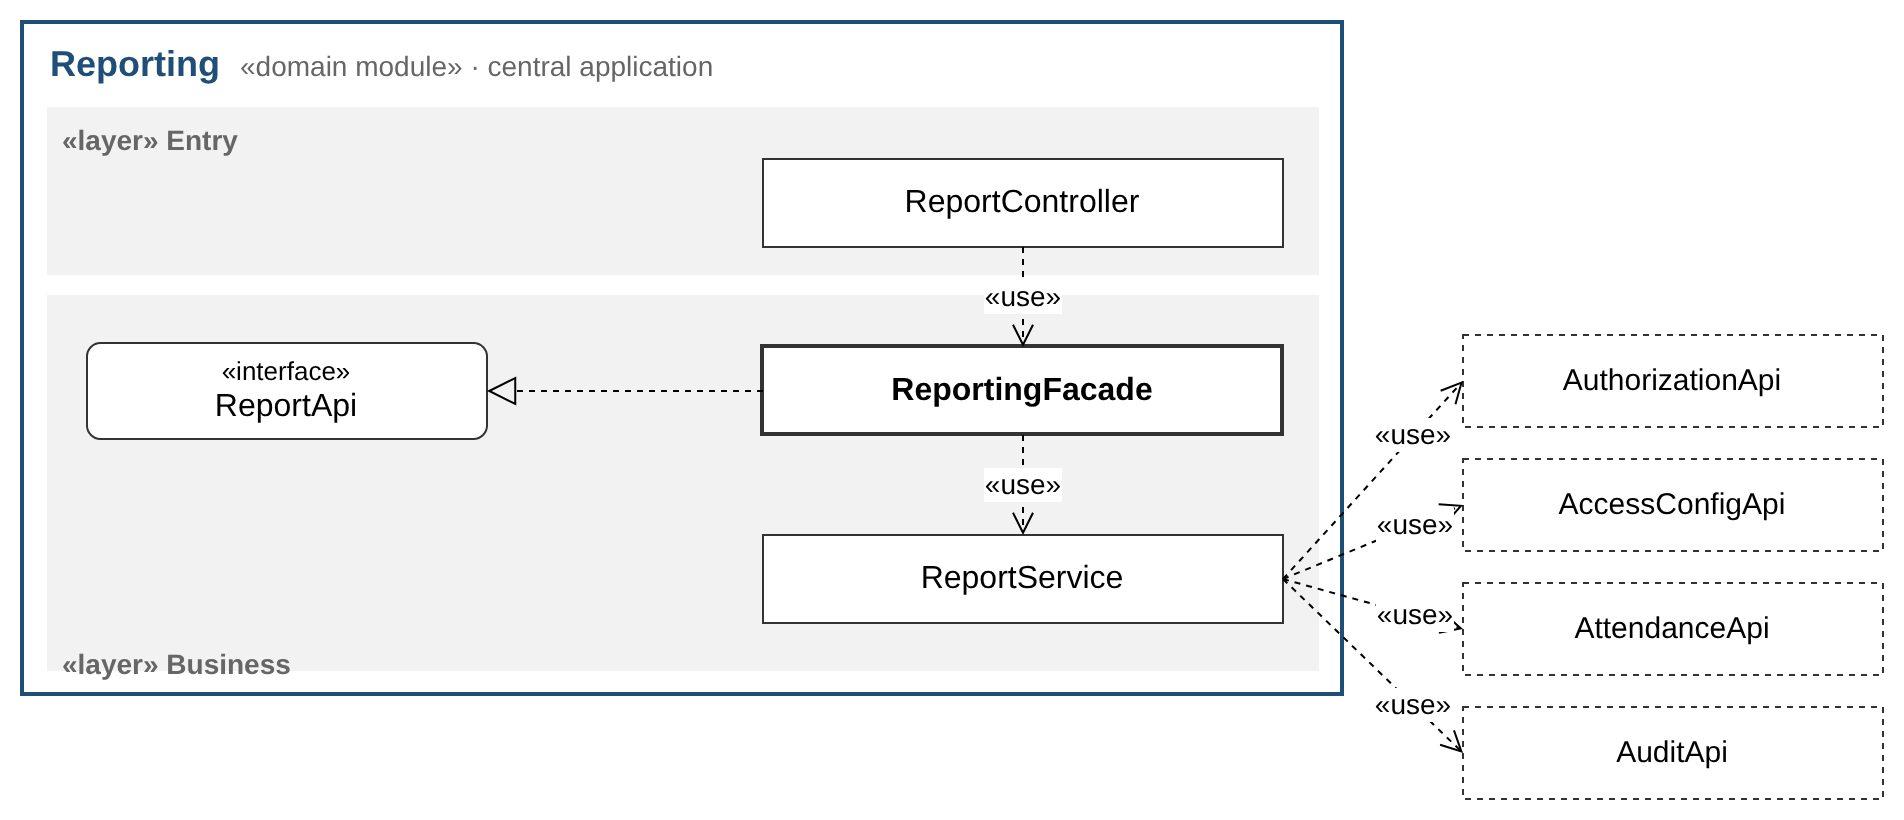
\includegraphics[width=450pt]{diagram/modules/figure-4-7-m6.png}

\vspace{6pt}
\textbf{Figure 4.7. M6 Reporting}
\phantomsection\addcontentsline{lof}{figure}{\protect\numberline{4.7}M6 Reporting}

\vspace{8pt}
{\small
\begin{tabular}{|>{\raggedright\arraybackslash}p{120pt}|>{\raggedright\arraybackslash}p{290pt}|}
\hline
\multicolumn{1}{|>{\columncolor{tableheader}\centering\arraybackslash}p{120pt}|}{\textbf{Component}} & \multicolumn{1}{>{\columncolor{tableheader}\centering\arraybackslash}p{290pt}|}{\textbf{Responsibility}} \\
\hline
ReportController, Facade & Implement ReportApi for both portals. \\
\hline
ReportService & Checks the scope through AuthorizationApi first, then reads access, attendance, and audit data. It keeps no copy of business data. \\
\hline
\end{tabular}
}

\vspace{6pt}
\textbf{Table 4.12. Components of M6 Reporting}
\phantomsection\addcontentsline{lot}{table}{\protect\numberline{4.12}Components of M6 Reporting}
\end{minipage}

\vspace{14pt}

\noindent\begin{minipage}{\linewidth}
Figure 4.8 shows the inside of Payroll Handover, and Table 4.13 describes its components.

\vspace{6pt}
\centering
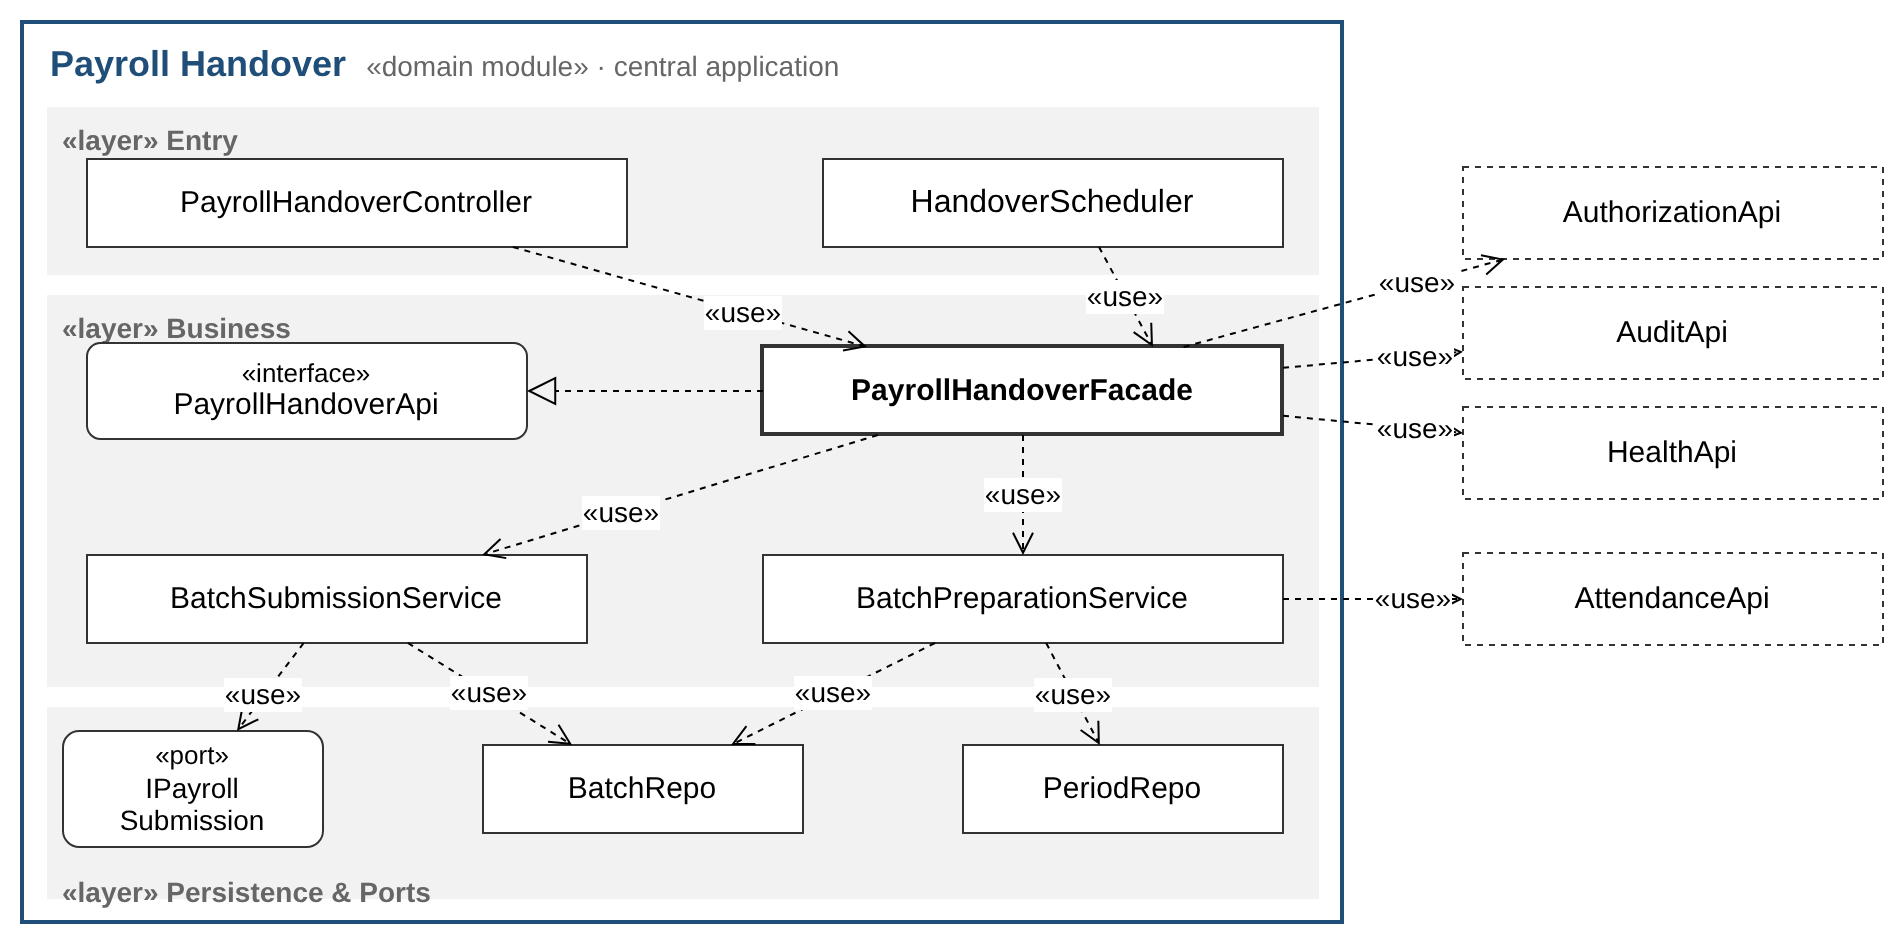
\includegraphics[width=450pt]{diagram/modules/figure-4-8-m7.png}

\vspace{6pt}
\textbf{Figure 4.8. M7 Payroll Handover}
\phantomsection\addcontentsline{lof}{figure}{\protect\numberline{4.8}M7 Payroll Handover}

\vspace{8pt}
{\small
\begin{tabular}{|>{\raggedright\arraybackslash}p{120pt}|>{\raggedright\arraybackslash}p{290pt}|}
\hline
\multicolumn{1}{|>{\columncolor{tableheader}\centering\arraybackslash}p{120pt}|}{\textbf{Component}} & \multicolumn{1}{>{\columncolor{tableheader}\centering\arraybackslash}p{290pt}|}{\textbf{Responsibility}} \\
\hline
Controller, HandoverScheduler & Accept manual actions and start the handover at 06:00 on day 1. \\
\hline
BatchPreparationService & Builds period and supplementary batches from attendance data. \\
\hline
BatchSubmissionService & Submits through IPayrollSubmission, queries the status where the API supports it, and stores CONFIRMED, REJECTED, or UNDETERMINED. \\
\hline
\end{tabular}
}

\vspace{6pt}
\textbf{Table 4.13. Components of M7 Payroll Handover}
\phantomsection\addcontentsline{lot}{table}{\protect\numberline{4.13}Components of M7 Payroll Handover}
\end{minipage}

\vspace{14pt}

\noindent\begin{minipage}{\linewidth}
Figure 4.9 shows the inside of HR/Payroll Integration, and Table 4.14 describes its components.

\vspace{6pt}
\centering
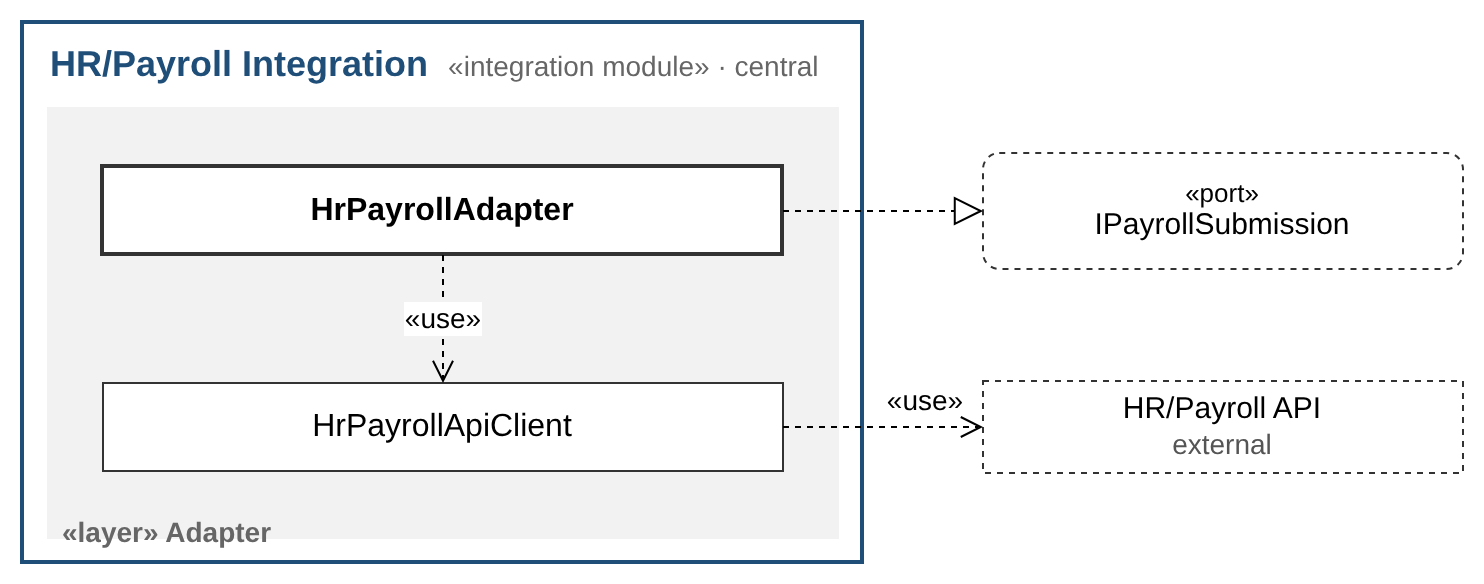
\includegraphics[width=350.3pt]{diagram/modules/figure-4-9-m8.png}

\vspace{6pt}
\textbf{Figure 4.9. M8 HR/Payroll Integration}
\phantomsection\addcontentsline{lof}{figure}{\protect\numberline{4.9}M8 HR/Payroll Integration}

\vspace{8pt}
{\small
\begin{tabular}{|>{\raggedright\arraybackslash}p{120pt}|>{\raggedright\arraybackslash}p{290pt}|}
\hline
\multicolumn{1}{|>{\columncolor{tableheader}\centering\arraybackslash}p{120pt}|}{\textbf{Component}} & \multicolumn{1}{>{\columncolor{tableheader}\centering\arraybackslash}p{290pt}|}{\textbf{Responsibility}} \\
\hline
HrPayrollAdapter & Implements IPayrollSubmission and translates batches and responses. \\
\hline
HrPayrollApiClient & Calls the HR/Payroll API and queries the status only if the API supports it (I-02). \\
\hline
\end{tabular}
}

\vspace{6pt}
\textbf{Table 4.14. Components of M8 HR/Payroll Integration}
\phantomsection\addcontentsline{lot}{table}{\protect\numberline{4.14}Components of M8 HR/Payroll Integration}
\end{minipage}

\vspace{14pt}

\noindent\begin{minipage}{\linewidth}
Figure 4.10 shows the inside of Site Sync, and Table 4.15 describes its components.

\vspace{6pt}
\centering
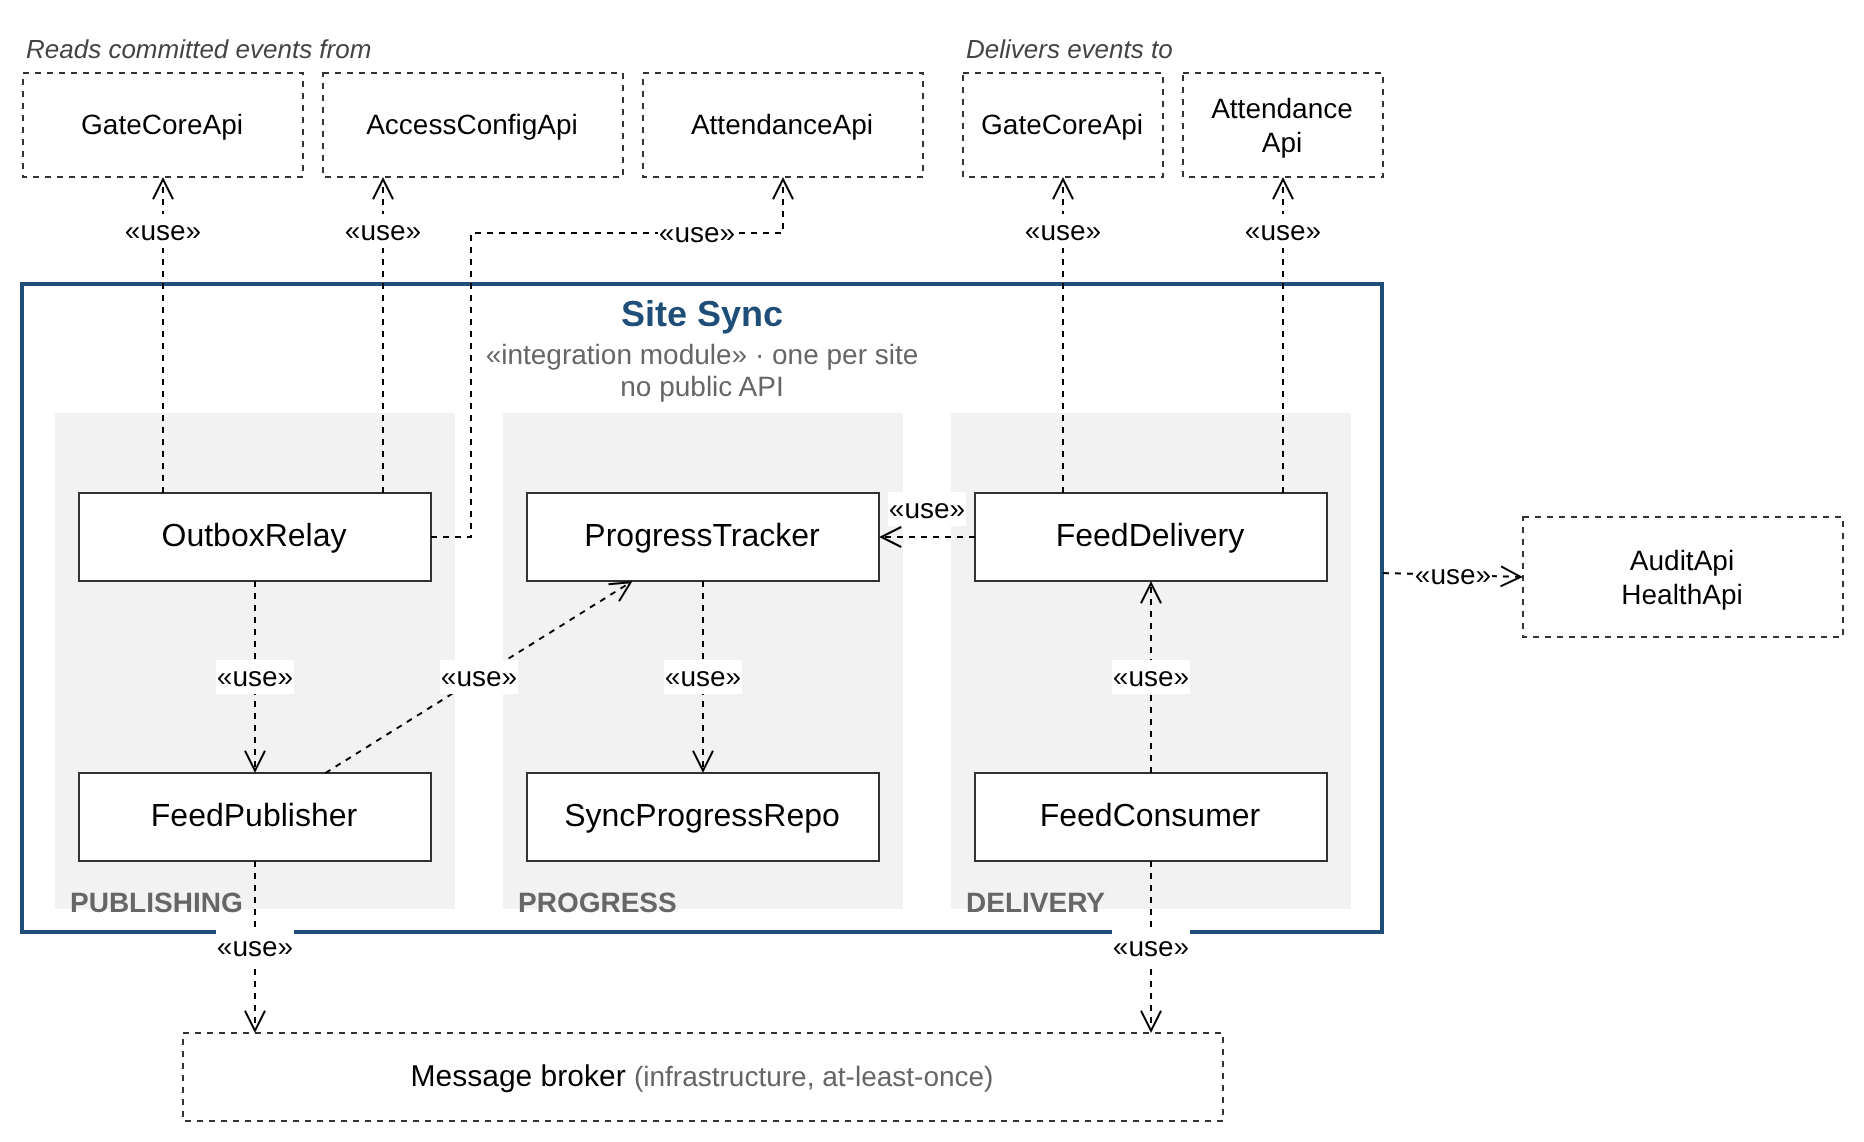
\includegraphics[width=440.5pt]{diagram/modules/figure-4-10-m9.png}

\vspace{6pt}
\textbf{Figure 4.10. M9 Site Sync}
\phantomsection\addcontentsline{lof}{figure}{\protect\numberline{4.10}M9 Site Sync}

\vspace{8pt}
{\small
\begin{tabular}{|>{\raggedright\arraybackslash}p{120pt}|>{\raggedright\arraybackslash}p{290pt}|}
\hline
\multicolumn{1}{|>{\columncolor{tableheader}\centering\arraybackslash}p{120pt}|}{\textbf{Component}} & \multicolumn{1}{>{\columncolor{tableheader}\centering\arraybackslash}p{290pt}|}{\textbf{Responsibility}} \\
\hline
OutboxRelay, FeedPublisher & Read committed events through the contracts of Gate Core, Access \& Configuration, and Attendance, and publish them with their original eventId. \\
\hline
FeedConsumer, FeedDelivery & Receive events from the broker and deliver them to Gate Core or Attendance; the acknowledgement is sent only after the receiver has stored the event. \\
\hline
ProgressTracker & Keeps watermarks and delivery progress and reports lag to Monitoring. \\
\hline
\end{tabular}
}

\vspace{6pt}
\textbf{Table 4.15. Components of M9 Site Sync}
\phantomsection\addcontentsline{lot}{table}{\protect\numberline{4.15}Components of M9 Site Sync}
\end{minipage}

\vspace{14pt}

\noindent\begin{minipage}{\linewidth}
Figure 4.11 shows the inside of Identity \& Access Control, and Table 4.16 describes its components.

\vspace{6pt}
\centering
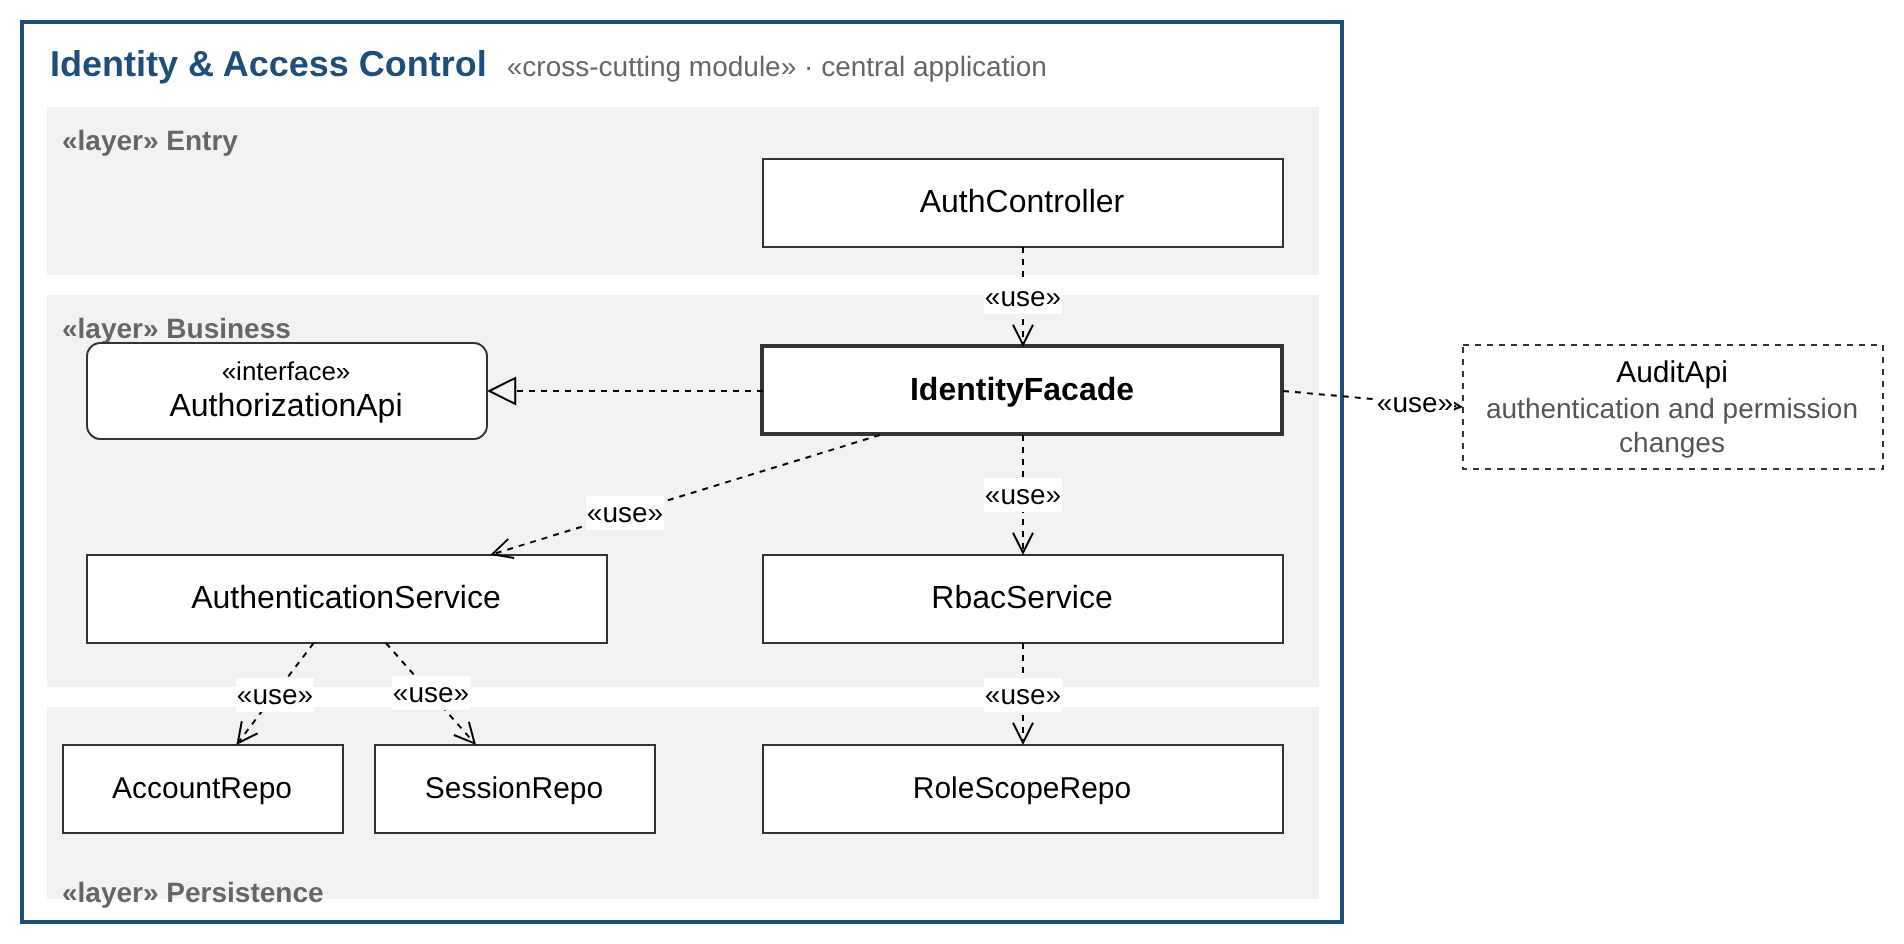
\includegraphics[width=450pt]{diagram/modules/figure-4-11-m10.png}

\vspace{6pt}
\textbf{Figure 4.11. M10 Identity \& Access Control}
\phantomsection\addcontentsline{lof}{figure}{\protect\numberline{4.11}M10 Identity \& Access Control}

\vspace{8pt}
{\small
\begin{tabular}{|>{\raggedright\arraybackslash}p{120pt}|>{\raggedright\arraybackslash}p{290pt}|}
\hline
\multicolumn{1}{|>{\columncolor{tableheader}\centering\arraybackslash}p{120pt}|}{\textbf{Component}} & \multicolumn{1}{>{\columncolor{tableheader}\centering\arraybackslash}p{290pt}|}{\textbf{Responsibility}} \\
\hline
AuthenticationService & Handles login and sessions. \\
\hline
RbacService & Manages roles and the action and data scope of each user. \\
\hline
IdentityFacade & Implements AuthorizationApi and sends authentication and permission-change evidence to Audit. \\
\hline
\end{tabular}
}

\vspace{6pt}
\textbf{Table 4.16. Components of M10 Identity \& Access Control}
\phantomsection\addcontentsline{lot}{table}{\protect\numberline{4.16}Components of M10 Identity \& Access Control}
\end{minipage}

\vspace{14pt}

\noindent\begin{minipage}{\linewidth}
Figure 4.12 shows the inside of Audit, and Table 4.17 describes its components.

\vspace{6pt}
\centering
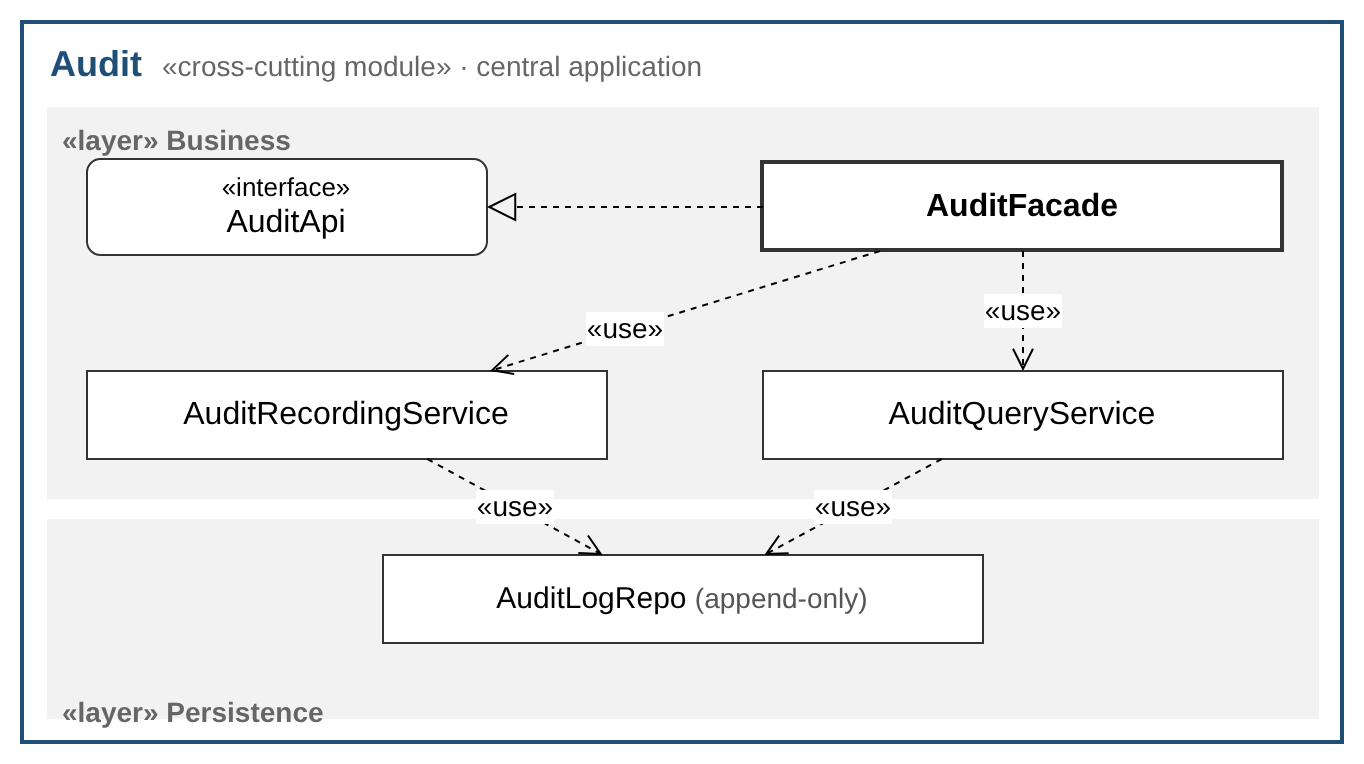
\includegraphics[width=321.8pt]{diagram/modules/figure-4-12-m11.png}

\vspace{6pt}
\textbf{Figure 4.12. M11 Audit}
\phantomsection\addcontentsline{lof}{figure}{\protect\numberline{4.12}M11 Audit}

\vspace{8pt}
{\small
\begin{tabular}{|>{\raggedright\arraybackslash}p{120pt}|>{\raggedright\arraybackslash}p{290pt}|}
\hline
\multicolumn{1}{|>{\columncolor{tableheader}\centering\arraybackslash}p{120pt}|}{\textbf{Component}} & \multicolumn{1}{>{\columncolor{tableheader}\centering\arraybackslash}p{290pt}|}{\textbf{Responsibility}} \\
\hline
AuditRecordingService & Appends audit records; existing records are never changed. \\
\hline
AuditQueryService & Answers queries that the caller has already scope-checked; Audit does not call Identity \& Access Control. \\
\hline
\end{tabular}
}

\vspace{6pt}
\textbf{Table 4.17. Components of M11 Audit}
\phantomsection\addcontentsline{lot}{table}{\protect\numberline{4.17}Components of M11 Audit}
\end{minipage}

\vspace{14pt}

\noindent\begin{minipage}{\linewidth}
Figure 4.13 shows the inside of Monitoring \& Operations, and Table 4.18 describes its components.

\vspace{6pt}
\centering
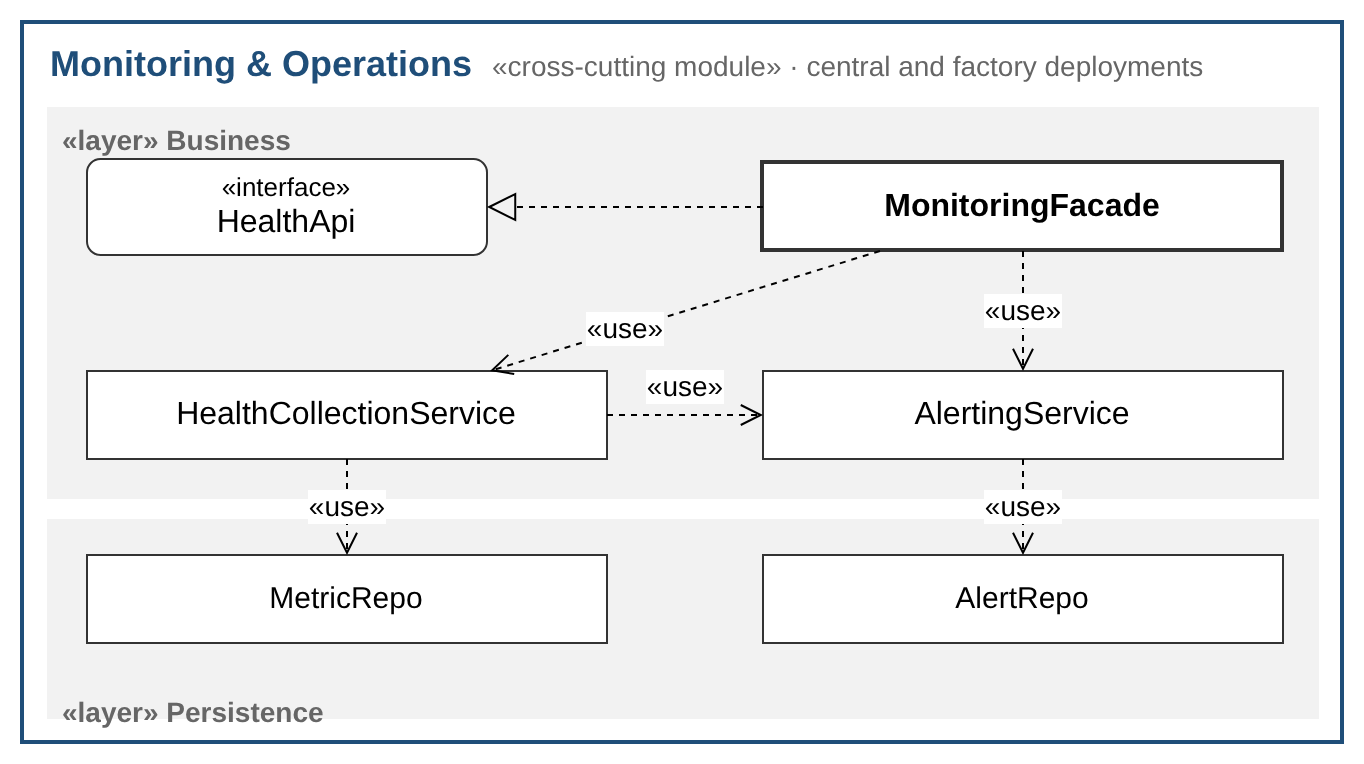
\includegraphics[width=321.8pt]{diagram/modules/figure-4-13-m12.png}

\vspace{6pt}
\textbf{Figure 4.13. M12 Monitoring \& Operations}
\phantomsection\addcontentsline{lof}{figure}{\protect\numberline{4.13}M12 Monitoring \& Operations}

\vspace{8pt}
{\small
\begin{tabular}{|>{\raggedright\arraybackslash}p{120pt}|>{\raggedright\arraybackslash}p{290pt}|}
\hline
\multicolumn{1}{|>{\columncolor{tableheader}\centering\arraybackslash}p{120pt}|}{\textbf{Component}} & \multicolumn{1}{>{\columncolor{tableheader}\centering\arraybackslash}p{290pt}|}{\textbf{Responsibility}} \\
\hline
MonitoringFacade & Implements HealthApi. It accepts reports from sources and returns the factory's current status and active alerts to Guard Status Display. \\
\hline
HealthCollectionService & Collects health, faults, latency, and progress. Sources report outside the scan response path, so Gate Core never waits for Monitoring. The factory deployment keeps working over the factory LAN when the WAN link is down and forwards its records to the central deployment when the link returns. \\
\hline
AlertingService & Raises alerts, for example on synchronization lag or a handover not confirmed by 10:00. \\
\hline
\end{tabular}
}

\vspace{6pt}
\textbf{Table 4.18. Components of M12 Monitoring \& Operations}
\phantomsection\addcontentsline{lot}{table}{\protect\numberline{4.18}Components of M12 Monitoring \& Operations}
\end{minipage}

\vspace{14pt}

\noindent\begin{minipage}{\linewidth}
Figure 4.14 shows the inside of Clients, and Table 4.19 describes its components.

\vspace{6pt}
\centering
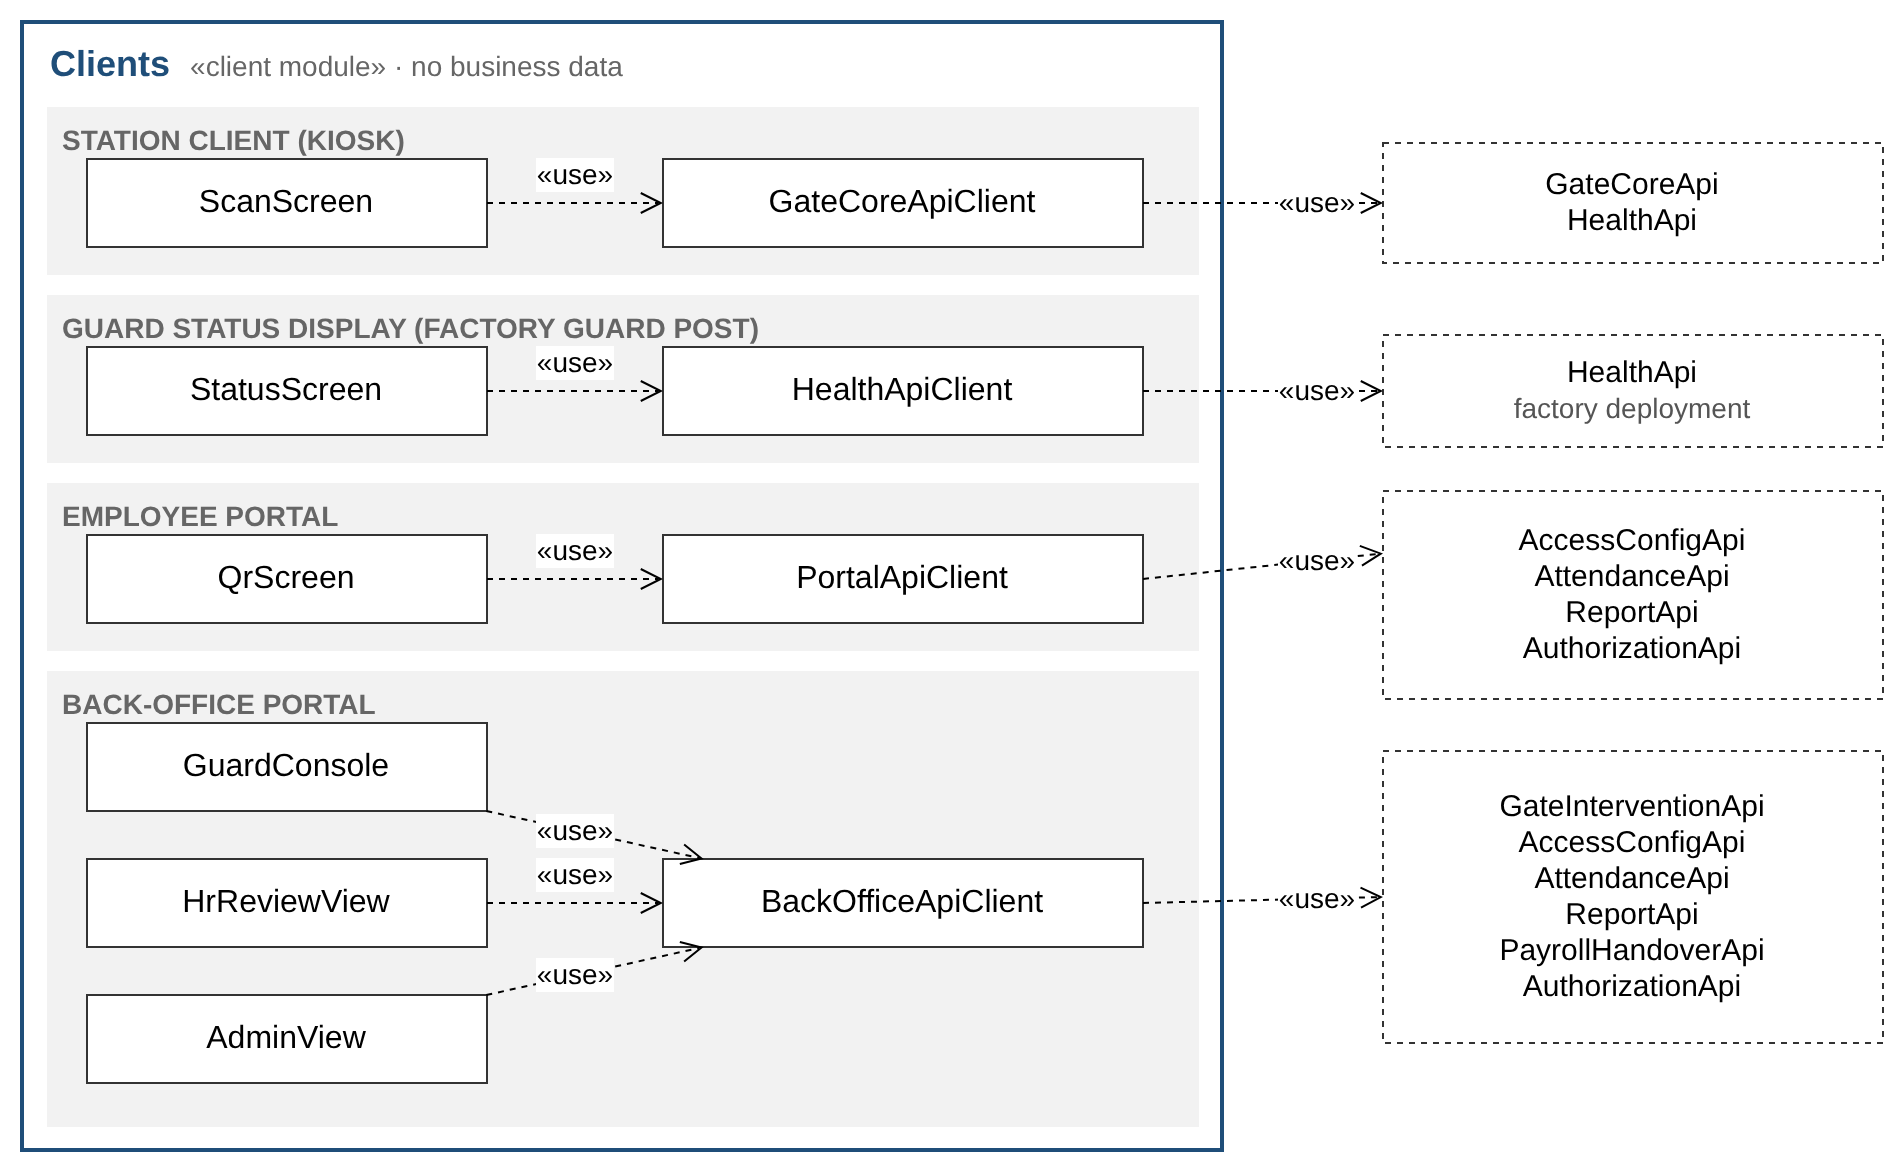
\includegraphics[width=450pt]{diagram/modules/figure-4-14-m13.png}

\vspace{6pt}
\textbf{Figure 4.14. M13 Clients}
\phantomsection\addcontentsline{lof}{figure}{\protect\numberline{4.14}M13 Clients}

\vspace{8pt}
{\small
\begin{tabular}{|>{\raggedright\arraybackslash}p{120pt}|>{\raggedright\arraybackslash}p{290pt}|}
\hline
\multicolumn{1}{|>{\columncolor{tableheader}\centering\arraybackslash}p{120pt}|}{\textbf{Component}} & \multicolumn{1}{>{\columncolor{tableheader}\centering\arraybackslash}p{290pt}|}{\textbf{Responsibility}} \\
\hline
Station Client & Shows the result, LANE BUSY, or UNDETERMINED, and calls getScanStatus with the same scanId after a timeout. \\
\hline
Employee Portal & Shows the QR screen and the employee's attendance history. \\
\hline
Back-office Portal & Provides the guard, HR, and administrator views. \\
\hline
Guard Status Display & A fixed screen at the factory guard post. It reads the factory's status and active alerts, such as degraded mode, from the factory deployment of Monitoring. It signs in with a device identity checked at the factory, so it works without central Identity \& RBAC, and it is read-only: assisted and emergency actions stay in Back-office Portal under the normal authorization rules. If it cannot reach the factory application, it shows that its data is stale. \\
\hline
\end{tabular}
}

\vspace{6pt}
\textbf{Table 4.19. Components of M13 Clients}
\phantomsection\addcontentsline{lot}{table}{\protect\numberline{4.19}Components of M13 Clients}
\end{minipage}

\vspace{14pt}

\subsection*{4.2. Component-and-Connector View}

\phantomsection
\addcontentsline{toc}{subsection}{4.2. Component-and-Connector View}

The C\&C View shows TMC at runtime: which components handle each request, which interfaces they call, and which connectors link the factory application, the central application, and the external systems. It consists of a component diagram, three runtime flows, and the states that keep these flows safe.

\subsubsection*{4.2.1. Component Diagram}

\phantomsection
\addcontentsline{toc}{subsubsection}{4.2.1. Component Diagram}

Figure 4.15 shows the runtime components of TMC and the connectors between them.

\noindent\begin{minipage}{\linewidth}
\centering
\IfFileExists{diagram/cc-view/figure-4-15-cc-view.png}{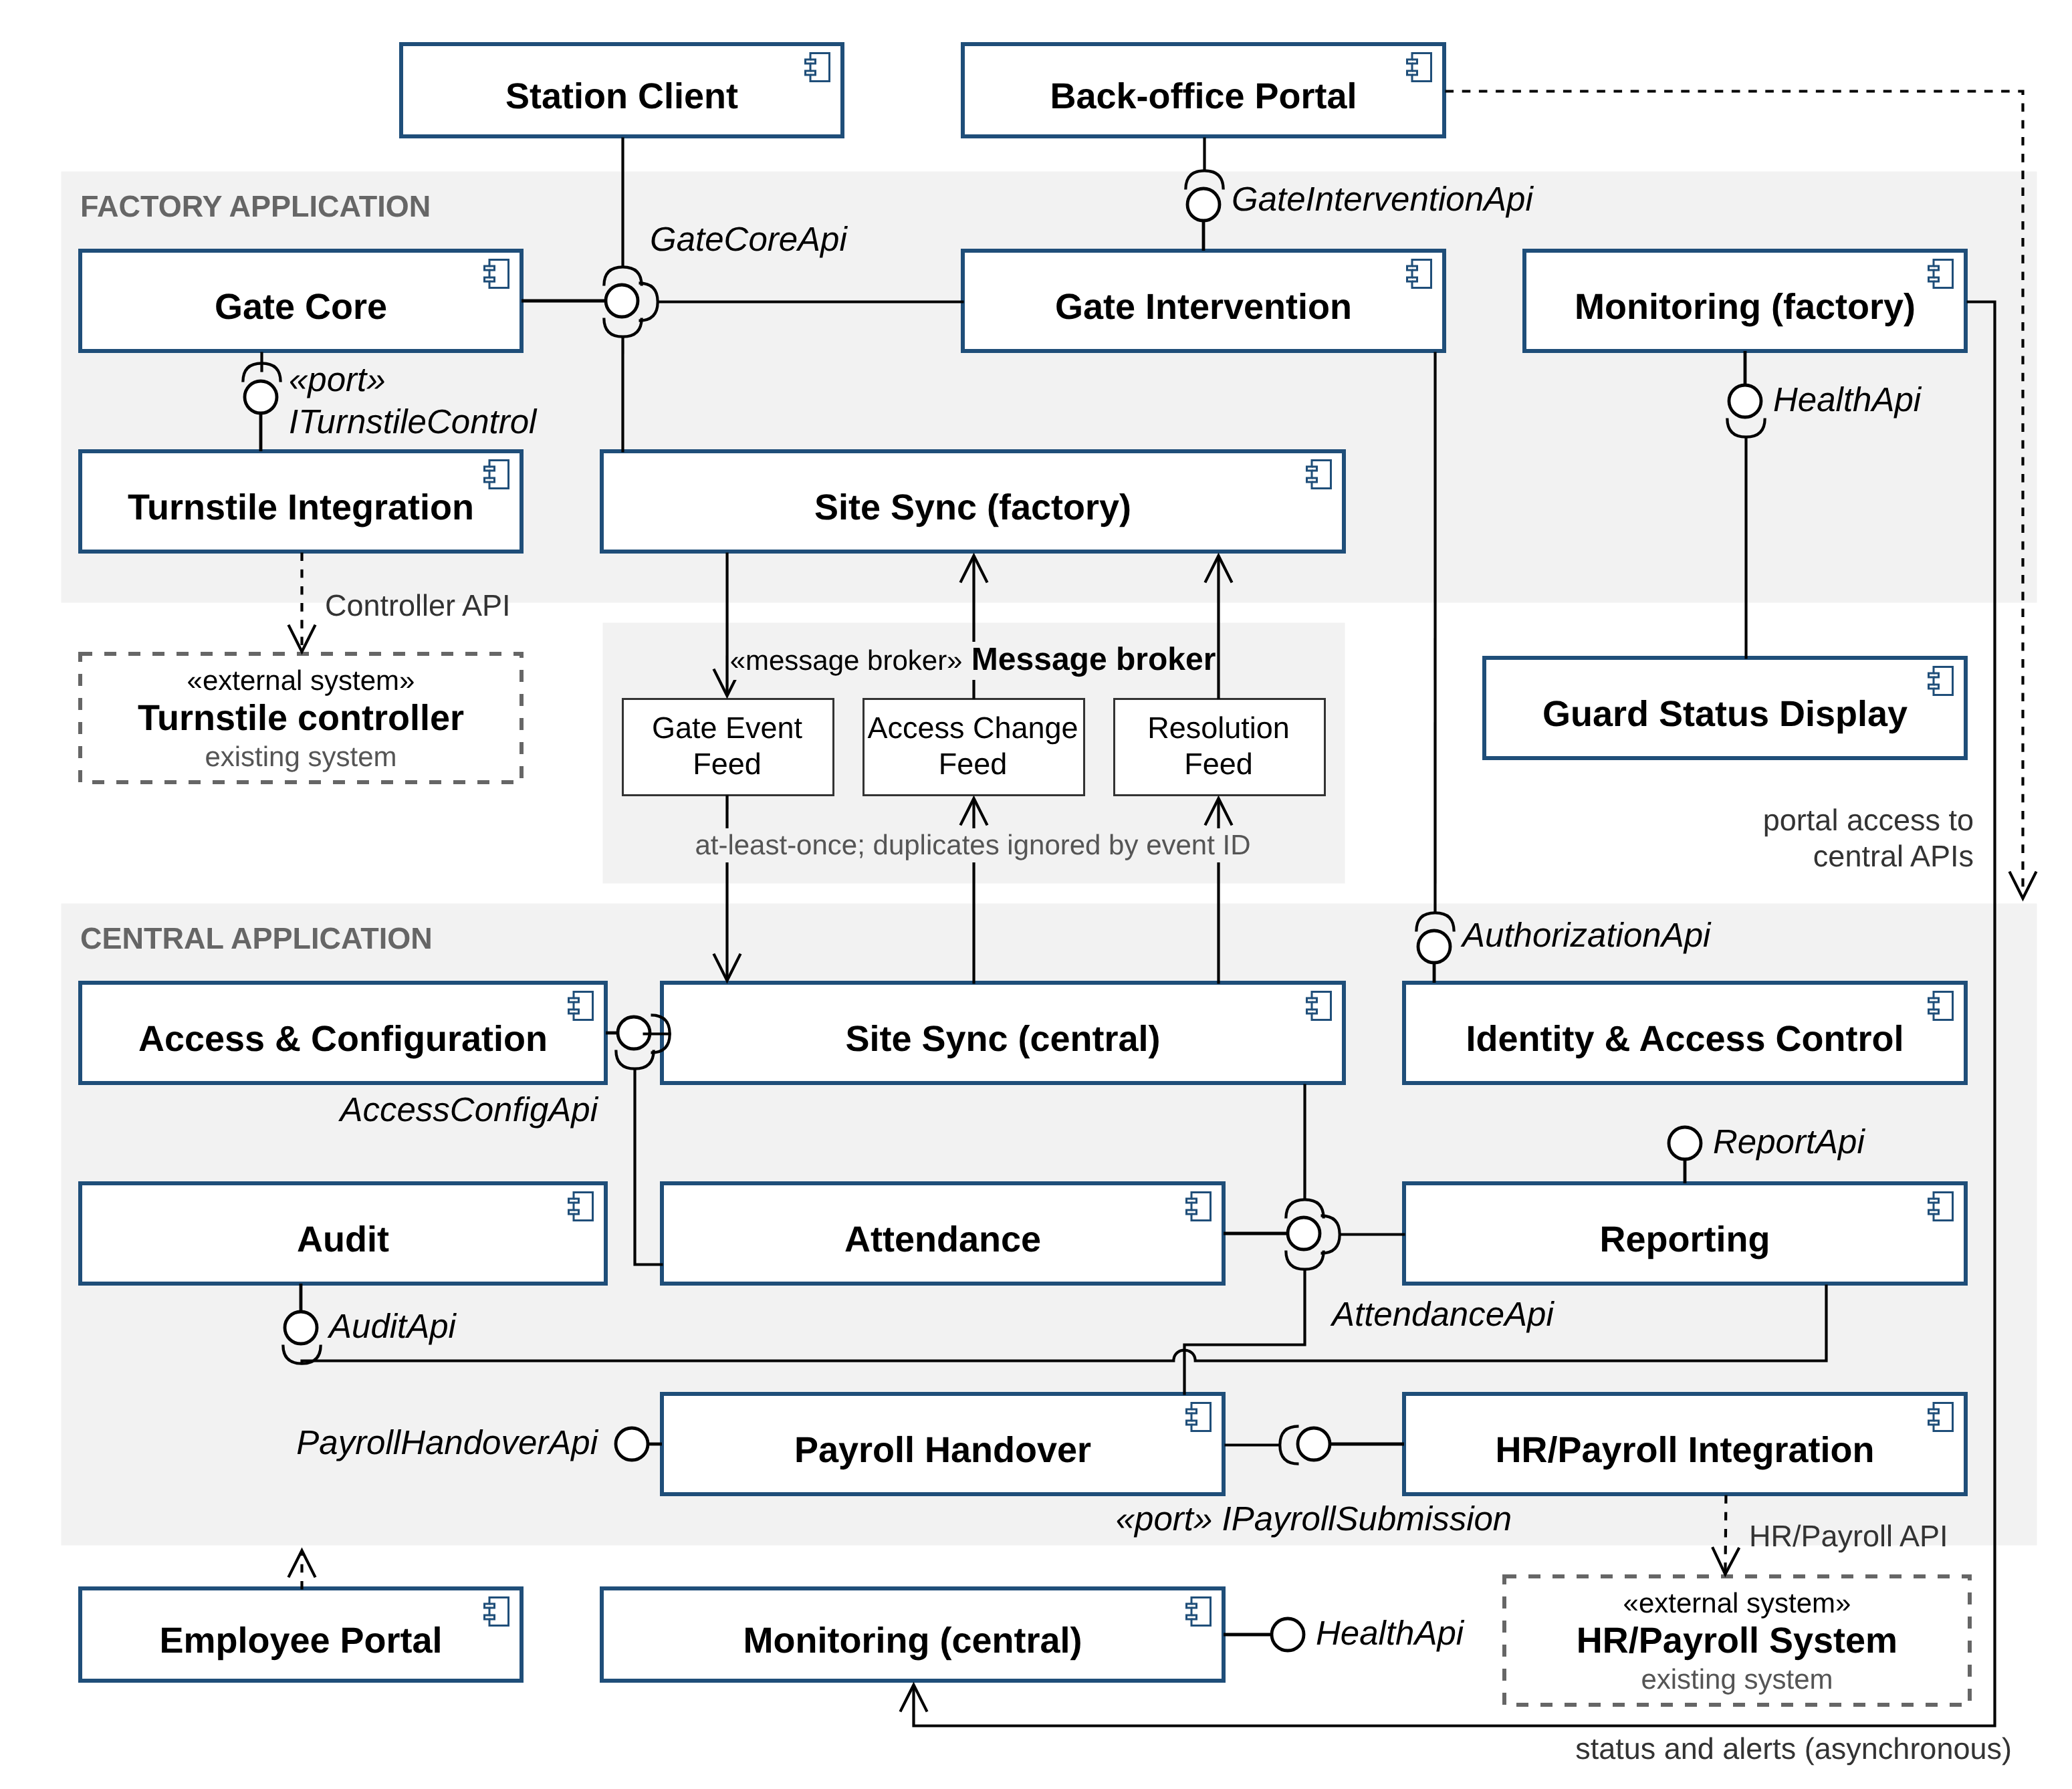
\includegraphics[width=450.0pt,height=620.0pt,keepaspectratio]{diagram/cc-view/figure-4-15-cc-view.png}}{\fbox{\parbox{300pt}{\centering\vspace{20pt}Figure being redrawn\vspace{20pt}}}}

\vspace{6pt}
\textbf{Figure 4.15. Component-and-Connector View of the TMC System}
\phantomsection\addcontentsline{lof}{figure}{\protect\numberline{4.15}Component-and-Connector View of the TMC System}
\end{minipage}

\medskip

\Needspace{6\baselineskip}
Figure 4.15 has five groups of elements:

\begin{itemize}[leftmargin=36pt, itemsep=2pt, topsep=4pt, parsep=2pt]
  \item \textbf{Clients:} Station Client on the kiosk sends scans through GateCoreApi. Employee Portal and Back-office Portal are separate clients for employees and staff. Guard Status Display on the guard screen reads the local HealthApi.
  \item \textbf{Factory application:} Gate Core, Turnstile Integration, Gate Intervention, the factory part of Site Sync, and factory Monitoring.
  \item \textbf{Central application:} Access \& Configuration, Attendance, Reporting, Payroll Handover, HR/Payroll Integration, Identity \& Access Control, Audit, and the central part of Site Sync. Central Monitoring runs outside both applications, on the monitoring server listed in Table 5.1.
  \item \textbf{Message broker:} carries three feeds with at-least-once delivery. Gate Event Feed takes scan events, transactions, assistance records, and ResolutionApplied from Gate Core to AttendanceApi. Access Change Feed takes versioned permissions, configuration, and verification keys from Access \& Configuration to Gate Core. Resolution Feed takes approved decisions linked to scans from Attendance Review to Gate Core.
  \item \textbf{External systems:} the turnstile controller, reached by Turnstile Adapter through the Controller API (I-01), and HR/Payroll, reached by HR/Payroll Adapter through the HR/Payroll API (I-02).
\end{itemize}

We draw the components in UML. Balls and half-circle sockets are provided and required interfaces, and a connected pair is a synchronous call. Solid open arrows are asynchronous transfers; factory Monitoring forwards status and alerts to central Monitoring separately from the broker. Dashed open arrows summarize portal access and external-system calls. To keep the figure readable, it leaves out the HealthApi reports and AuditApi appends of source components, the handover scheduler, Reporting's AccessConfigApi call, and TMC email integration.

\textbf{Interfaces and ports.} Table 4.20 lists the public APIs and integration contracts. The owner defines the contract. Turnstile Adapter implements the outgoing command ports, grouped as ITurnstileControl. Gate Core implements the separate incoming port IPassageEvents, which the adapter calls. Each API name stands for a group of operations, and a consumer only uses the ones it needs.

{\small
\begin{longtable}{|>{\raggedright\arraybackslash}p{92pt}|>{\raggedright\arraybackslash}p{68pt}|>{\raggedright\arraybackslash}p{132pt}|>{\raggedright\arraybackslash}p{105pt}|}
\hline
\multicolumn{1}{|>{\columncolor{tableheader}\centering\arraybackslash}p{92pt}|}{\textbf{API or port}} & \multicolumn{1}{>{\columncolor{tableheader}\centering\arraybackslash}p{68pt}|}{\textbf{Owner}} & \multicolumn{1}{>{\columncolor{tableheader}\centering\arraybackslash}p{132pt}|}{\textbf{Main operations}} & \multicolumn{1}{>{\columncolor{tableheader}\centering\arraybackslash}p{105pt}|}{\textbf{Consumers}} \\
\hline
\endhead
\multicolumn{4}{c}{\rule{0pt}{22pt}\normalsize\textbf{Table 4.20. Public Interfaces and Integration Ports}} \\
\endlastfoot
GateCoreApi & Gate Core (M1) & submitScan, getScanStatus; recordIntervention, requestAssistedOpen, requestEmergencyRelease, requestEmergencyReset; applyEligibilityChanges, applyScanResolution; read committed Gate Event Feed events & Station Client; Gate Intervention; Site Sync \\
\hline
GateInterventionApi & Gate Intervention (M3) & recordAssistedAccess, authorizeAssistedOpen, emergencyRelease, resetEmergency & Back-office Portal \\
\hline
AccessConfigApi & Access \& Configuration (M4) & issue fresh QR; request email display link; manage rights, stations, shifts, and rules; read committed Access Change Feed events & Employee Portal; Back-office Portal; Attendance; Reporting; Site Sync \\
\hline
AttendanceApi & Attendance (M5) & receive events; review and approve cases; query period data and open cases; read committed Resolution Feed events & Site Sync; Employee Portal; Back-office Portal; Reporting; Payroll Handover \\
\hline
ReportApi & Reporting (M6) & query attendance, reports, and authorized audit data & Employee Portal; Back-office Portal \\
\hline
PayrollHandoverApi & Payroll Handover (M7) & start period, query progress, prepare supplementary handover & Scheduler; Back-office Portal \\
\hline
AuthorizationApi & Identity \& Access Control (M10) & check identity, action, and data scope; administer accounts separately & Business components; Employee Portal; Back-office Portal \\
\hline
AuditApi & Audit (M11) & append source evidence; query authorized history & Source components; Reporting \\
\hline
HealthApi & Monitoring \& Operations (M12) & report health, faults, latency, and progress; read the factory's current status and active alerts & Report: Station Client; Gate Core; Turnstile Integration; Site Sync; Payroll Handover. Read: Guard Status Display \\
\hline
Turnstile ports & Gate Core (M1) & ITurnstileControl groups openGate (IOpenGate), closeGate (ICloseGate), and emergencyRelease/resetEmergency (IEmergencyGate), all returning results. IPassageEvents carries PASSAGE and LANE\_CLEAR. Status query is optional. & M2 implements command ports; M1 uses them. M1 implements IPassageEvents; M2 calls it \\
\hline
IPayrollSubmission & Payroll Handover (M7) & submit batch, receive outcome, inquire where supported & Payroll Handover uses; implemented by HR/Payroll Integration (M8) \\
\hline
\end{longtable}
}
\phantomsection\addcontentsline{lot}{table}{\protect\numberline{4.20}Public Interfaces and Integration Ports}

\Needspace{6\baselineskip}
Three rules apply across these interfaces:

\begin{itemize}[leftmargin=36pt, itemsep=2pt, topsep=4pt, parsep=2pt]
  \item \textbf{Permissions per operation.} Using an API group does not give a consumer every operation in it; authorization is checked where the request is processed. Station Client can submit and query scans but cannot call recordIntervention, and Employee Portal cannot approve cases.
  \item \textbf{Events through contracts.} Site Sync reads committed events through source-owned contracts and keeps their event IDs and versions; it never reads module repositories. Receivers use event IDs, object IDs, and versions to ignore duplicates and to spot missing or out-of-order data.
  \item \textbf{Internal calls stay internal.} Calls inside one module, such as Gate Transaction Processor to Access Decision or Attendance Review to Attendance Consolidation, are not public interfaces and are not listed in Table 4.20.
\end{itemize}

\Needspace{6\baselineskip}
\textbf{Data ownership.} Each kind of data has one owner, and other modules reach it only through that owner's interface:

\begin{itemize}[leftmargin=36pt, itemsep=2pt, topsep=4pt, parsep=2pt]
  \item Gate Core: scan states, transactions originating at gates, assistance records received at their source, and Eligibility Snapshot.
  \item Access \& Configuration: employee information, factory access permissions, station and lane configuration, shift schedules, and aggregation rules.
  \item Attendance: consolidated attendance data, review records, and decisions. Attendance Consolidation updates attendance outcomes; Attendance Review manages cases and approvals.
  \item Payroll Handover: handover periods, batch content, and acknowledgement evidence.
  \item Audit: audit data received from sources.
  \item Identity \& Access Control: accounts, roles, system access permissions, and login sessions.
  \item Monitoring \& Operations: monitoring information, faults, alerts, and operational task progress.
\end{itemize}

Gate Intervention never writes Gate Core's data directly; it asks Gate Core through recordIntervention and the assisted and emergency requests.

\textbf{External contracts.} For the controller, we use the results and events assumed in I-01 and I-05. Each of OPEN\_CONFIRMED, PASSAGE, LANE\_CLEAR, and CLOSED is reported for a given lane and command. OPEN\_CONFIRMED and CLOSED come back as command results, while PASSAGE and LANE\_CLEAR arrive later as separate events. Gate Core sends closeGate once after LANE\_CLEAR, and the controller's own interlock must still prevent unsafe closing. After an emergency release, closing also needs an authorized reset and confirmation that release mode has ended. If any of these confirmations is missing, Gate Core alerts the guard and leaves recovery to the approved safety procedure. Email Link Sender sends only a link through TMC's email service, never a QR image, and the employee signs in before seeing a fresh code (I-08); an email failure does not affect the app or the web portal. Signals, status inquiry, acknowledgement, and duplicate handling must all be checked against the real APIs.

\noindent\begin{minipage}{\linewidth}
Table 4.21 summarizes the connector types.

\vspace{8pt}
\centering
\begin{tabular}{|>{\raggedright\arraybackslash}p{83.5pt}|>{\raggedright\arraybackslash}p{155.5pt}|>{\raggedright\arraybackslash}p{170.5pt}|}
\hline
\multicolumn{1}{|>{\columncolor{tableheader}\centering\arraybackslash}p{83.5pt}|}{\textbf{Type}} & \multicolumn{1}{>{\columncolor{tableheader}\centering\arraybackslash}p{155.5pt}|}{\textbf{Used In}} & \multicolumn{1}{>{\columncolor{tableheader}\centering\arraybackslash}p{170.5pt}|}{\textbf{Meaning}} \\
\hline
Synchronous call & Clients to interfaces; components to functions requiring results; internal module calls & The caller waits for the result before continuing. \\
\hline
Asynchronous event channel & Gate Event Feed; Access Change Feed; Resolution Feed; audit and operational information transfer & Recipients process at their own pace, with appropriate acknowledgements and duplicate prevention. \\
\hline
Port implementation & Turnstile Adapter with the turnstile command ports; Gate Core with IPassageEvents; HR/Payroll Adapter with IPayrollSubmission & A contract relationship between an adapter and the module defining the port; not a business message. \\
\hline
External system call & Adapters to the controller or HR/Payroll & Subject to external API conditions for timeouts, responses, inquiries, and resubmissions. \\
\hline
\end{tabular}

\vspace{6pt}
\textbf{Table 4.21. Connector Types}
\phantomsection\addcontentsline{lot}{table}{\protect\numberline{4.21}Connector Types}
\end{minipage}

\medskip

\Needspace{6\baselineskip}
Four points of the design are visible in Figure 4.15:

\begin{itemize}[leftmargin=36pt, itemsep=2pt, topsep=4pt, parsep=2pt]
  \item \textbf{Short synchronous path.} Only Station Client, Gate Core, and Turnstile Adapter are on the path the kiosk waits for, and all of them are in the factory. Reporting, handover, and synchronization are outside this response path; shared-resource contention still needs limits and performance tests (AC-03). Once the confirmed opening is stored, passage recording and safe closure run independently of the kiosk result.
  \item \textbf{Events between sites.} Business data between a factory and the central site moves only through the three feeds, so a WAN outage delays this data instead of stopping the QR flow, within the limits of I-10 (AC-01, AC-02). The exception is assisted and emergency opening, which waits synchronously for Identity \& RBAC at the central site (Table 3.2).
  \item \textbf{One adapter per external system.} The controller and HR/Payroll are each reached through one adapter, so an API change stays inside that adapter (AC-06).
  \item \textbf{Audit at the source.} Each source records audit evidence before sending it asynchronously to Audit Log, and Reporting checks authorization before calling AuditApi.query (AC-05). Chapter 7 covers what is audited and how long it is kept.
\end{itemize}

\clearpage
\subsubsection*{4.2.2. Flow A: QR Scan, Opening, Passage and Closure}

\phantomsection
\addcontentsline{toc}{subsubsection}{4.2.2. Flow A: QR Scan, Opening, Passage and Closure}

Figure 4.16 shows the gate flow for one scan, from the kiosk to the safe closure of the lane. The 2-second target of NFR-01 ends when the kiosk displays the result.

\noindent\begin{minipage}{\linewidth}
\centering
\IfFileExists{diagram/sequence/figure-4-16-qr-scan.png}{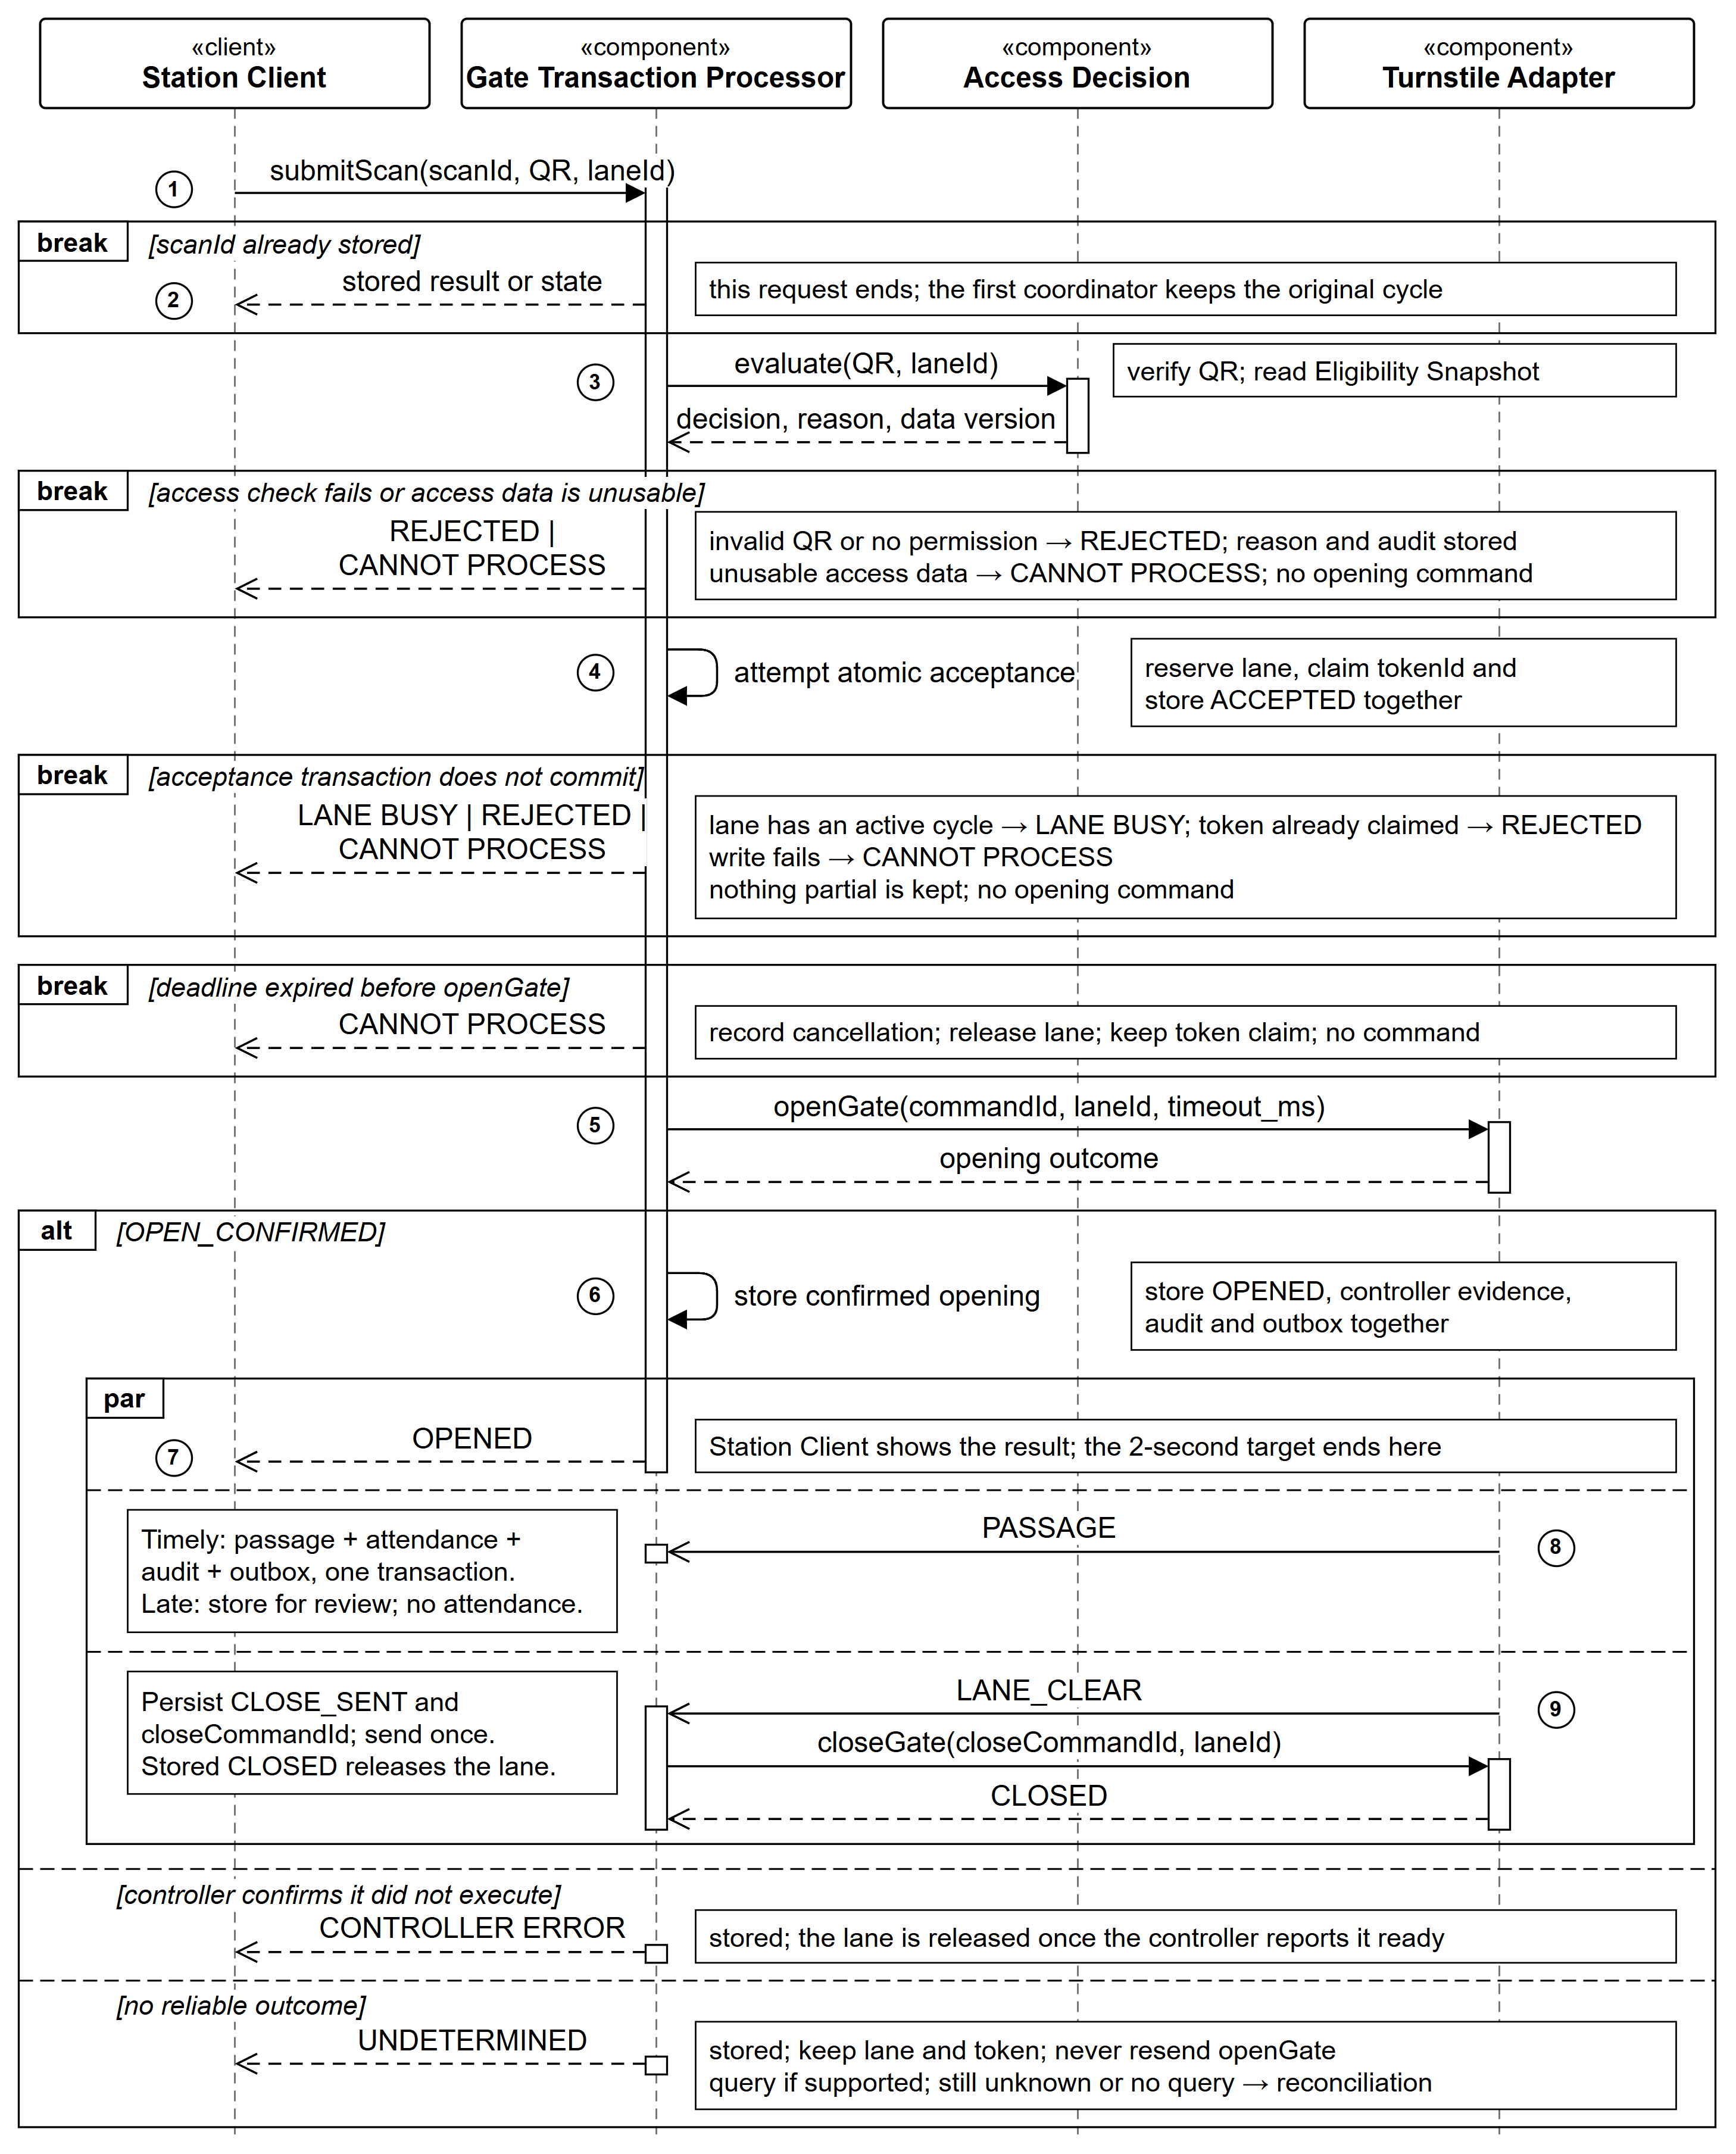
\includegraphics[width=450.0pt,height=555.0pt,keepaspectratio]{diagram/sequence/figure-4-16-qr-scan.png}}{\fbox{\parbox{300pt}{\centering\vspace{20pt}Figure being redrawn\vspace{20pt}}}}

\vspace{6pt}
\textbf{Figure 4.16. QR Scan Sequence --- Validation, Opening, Passage and Closure}
\phantomsection\addcontentsline{lof}{figure}{\protect\numberline{4.16}QR Scan Sequence --- Validation, Opening, Passage and Closure}
\end{minipage}

\vspace{8pt}

\Needspace{6\baselineskip}
Solid arrows with filled heads are synchronous calls, solid open arrows are signals, and dashed open arrows are returns; PASSAGE and LANE\_CLEAR come from the controller through Turnstile Adapter as events, and CLOSED comes back as the result of closeGate. Four break fragments stop the flow on a duplicate request, a failed check or unusable access data, a failed acceptance write, and a deadline that expires before the opening command. The alt fragment separates OPENED, CONTROLLER ERROR, and UNDETERMINED, and only OPENED contains the par fragment for the kiosk result, passage, and closing. The circled numbers 1--9 match steps A1--A9:

\begin{itemize}[leftmargin=30pt, labelwidth=24pt, labelsep=6pt, align=left, itemsep=3pt, topsep=4pt, parsep=2pt]
  \item[\textbf{A1}] \textbf{Station intake.} Station Client reads the QR code, records the start time, creates a scanId, and calls GateCoreApi.submitScan. Every later exchange about this scan keeps the same scanId.
  \item[\textbf{A2}] \textbf{Duplicate check.} Gate Transaction Processor checks whether the scan already exists and, if so, returns the stored result or state. For a new scan, only one coordinator may issue the opening command, even when requests arrive at the same time.
  \item[\textbf{A3}] \textbf{Access checks.} Access Decision verifies the QR code and its validity, then reads Eligibility Snapshot for employee status, factory permission, and lane configuration. It returns the decision, the reason, and the data version it used.
  \item[\textbf{A4}] \textbf{Reserve the lane and store ACCEPTED.} If the checks pass, Gate Transaction Processor reserves the lane, claims the tokenId, and stores ACCEPTED in one transaction. If the lane already has an active or unresolved gate cycle, it returns LANE BUSY without claiming the token. If the write fails or the token is already claimed, no opening command is sent.
  \item[\textbf{A5}] \textbf{Opening command.} Just before the command, Gate Transaction Processor recomputes how much of the scan deadline is left. If nothing is left, it sends no command: the scan becomes CANNOT PROCESS with reason \texttt{OPEN\_DEADLINE\_EXPIRED\_}\allowbreak\texttt{BEFORE\_COMMAND}, the lane is released, and the token stays claimed. Otherwise it calls openGate through IOpenGate with a commandId linked to the scan and a time limit of 700 ms or the remaining deadline, whichever is shorter (Table 5.5). A receipt from the controller does not mean the gate opened.
  \item[\textbf{A6}] \textbf{Opening result.} On OPEN\_CONFIRMED, Gate Transaction Processor stores the OPENED state, the controller evidence, audit data, and an outbox event. An explicit non-execution is stored as CONTROLLER ERROR. An uncertain outcome is stored as UNDETERMINED first, and the lane and token stay reserved. Gate Core queries the same commandId once where supported and records a definite result. If the answer is still unclear or no query is supported, the scan moves to PENDING RECONCILIATION. The command is never resent to test it.
  \item[\textbf{A7}] \textbf{Kiosk result.} Station Client shows the opening result, which ends the NFR-01 measurement. It does not tell the employee that attendance has been recorded.
  \Needspace{5\baselineskip}
  \item[\textbf{A8}] \textbf{Passage and attendance.} For the first reliable passage linked to a QR scan's command and lane and received within the observation window while the scan is still OPENED (not already sent to reconciliation, for example by an emergency release), Gate Transaction Processor stores that event with at most one original attendance transaction per scanId (employee, Vietnam time, direction, factory, lane, source), audit data, and an outbox event in one write. Site Sync later sends the event to Attendance. A repeated event is ignored, and a second, different passage for the same scan is flagged for review. Without reliable passage evidence, the opening stays recorded and the case goes to reconciliation. If PASSAGE only arrives after the 15-second observation has ended (NO\_PASSAGE), Gate Core stores it once with an audit record and marks it LATE\_PASSAGE, but creates no attendance transaction; Attendance Review decides the case.
  \item[\textbf{A9}] \textbf{Safe closure.} When the controller reports LANE\_CLEAR, Gate Transaction Processor sends closeGate once, whether passage was recorded or not, and stores CLOSED only after the controller confirms it. It stores CLOSE\_SENT and the closeCommandId before sending, so a repeated LANE\_CLEAR only checks that command and never creates a second one. If LANE\_CLEAR or CLOSED is not confirmed, it alerts the guard and keeps the lane reserved until one of the safe-release conditions below is met; attendance backed by a passage event stays recorded.
\end{itemize}

Under I-09, each QR code is valid for 60 seconds at one factory and can be claimed by only one ACCEPTED scan.

\Needspace{6\baselineskip}
\textbf{Lane rules.} Duplicate checks on scanId do not stop two employees from scanning at the same lane, so each lane follows these rules:

\begin{itemize}[leftmargin=36pt, itemsep=2pt, topsep=4pt, parsep=2pt]
  \item A lane has at most one active normal gate cycle, from ACCEPTED until the lane is released.
  \item Reserving the lane, claiming the token, and storing ACCEPTED happen in one atomic write, for example under a unique constraint on the lane's active cycle. A separate check-then-reserve step would let two scans pass together.
  \item If the lane is busy, Gate Core claims no token, sends no openGate, and returns LANE BUSY.
  \item Resending the same scanId returns the stored result. Scanning again after the lane is free creates a new scanId; the same QR code works only if it is unclaimed and still valid.
  \item If a deadline expires before any opening command is sent, Gate Core records CANNOT PROCESS and releases the unused lane reservation, keeping the token claim. Once a command may have been sent, release requires confirmed CLOSED, explicit non-execution with the lane ready, or restoration by a guard. A timeout or the end of the passage observation alone never releases that lane.
\end{itemize}

Because a lane stays reserved for the whole cycle, the number of lanes must be checked against the peak load. A fast LANE BUSY answer proves neither a successful opening within 2 seconds nor enough lane capacity; the lane count is confirmed in the site survey.

\Needspace{9\baselineskip}
\textbf{Failure paths.} Table 4.22 shows failure handling and its effect on attendance.

\begin{longtable}{|>{\raggedright\arraybackslash}p{114.5pt}|>{\raggedright\arraybackslash}p{194.5pt}|>{\raggedright\arraybackslash}p{102.5pt}|}
\hline
\multicolumn{1}{|>{\columncolor{tableheader}\centering\arraybackslash}p{114.5pt}|}{\textbf{Case}} & \multicolumn{1}{>{\columncolor{tableheader}\centering\arraybackslash}p{194.5pt}|}{\textbf{Handling}} & \multicolumn{1}{>{\columncolor{tableheader}\centering\arraybackslash}p{102.5pt}|}{\textbf{Attendance Outcome}} \\
\hline
\endhead
\multicolumn{3}{c}{\rule{0pt}{20pt}\normalsize\textbf{Table 4.22. Alternative and Failure Paths in the Scanning Flow}} \\
\endlastfoot
Invalid or expired QR code, suspended or unauthorized employee, or token already claimed & Reject without a command; store the reason and audit evidence. & Not created. \\
\hline
Same scan resubmitted, or concurrent requests for it & Return the stored state or result; only one coordinator handles the command. & No extra transaction. \\
\hline
New scan (new scanId) on a free lane & Treat as a new scan, even if it comes soon after another. & Only after its own passage event. \\
\hline
New scan while the lane is busy or its last cycle is unresolved & Return LANE BUSY; claim no token and send no openGate. & Not created. \\
\hline
Cannot store ACCEPTED & Stop before the command; return CANNOT PROCESS. & Not created. \\
\hline
Scan deadline passes after ACCEPTED but before openGate & Send no command; store CANNOT PROCESS with reason \texttt{OPEN\_DEADLINE\_EXPIRED\_}\allowbreak\texttt{BEFORE\_COMMAND} and release the lane. The token stays claimed, so the same QR code cannot be used again. & Not created. \\
\hline
Access data older than 60 seconds but less than 30 minutes since the last confirmed update, and the other degraded-mode conditions met (I-10) & Continue in degraded mode; flag the scan and transaction DEGRADED. & After passage, flagged. \\
\hline
Access data 30 minutes old or more, incomplete, or with a gap, or another required condition fails & Stop automatic decisions; return CANNOT PROCESS. & Not created. \\
\hline
Controller confirms it did not execute & Store the failure and return an error. & Not created. \\
\hline
Timeout or lost response after the command may have been sent & Store UNDETERMINED and keep the lane and token; query status once where supported, otherwise move to PENDING RECONCILIATION. Never resend. & Not yet created. \\
\hline
Gate opened but the outcome cannot be stored & Do not report success; recover from controller evidence without resending. & Depends on passage evidence. \\
\hline
Station Client gets no response & Show UNDETERMINED; inquire with the same scanId. & Depends on passage or reconciliation. \\
\hline
Opening confirmed, passage missing or uncertain & Keep the opening; send the case to reconciliation. & Not created automatically. \\
\hline
LANE\_CLEAR or CLOSED not confirmed & Alert the guard; query the stored close command where supported. Do not resend it automatically. & A confirmed passage stays. \\
\hline
Employee has no QR code & Store an authorized support case first, then an assisted openGate. & Only after HR approval. \\*
\hline\noalign{\nobreak}
Emergency opening while a scan is OPENED & Put the lane on EMERGENCY\_HOLD and send unresolved scans to reconciliation; reset and close under the safety procedure. & Earlier passage stays; release itself creates none. \\
\hline
\end{longtable}
\phantomsection\addcontentsline{lot}{table}{\protect\numberline{4.22}Alternative and Failure Paths in the Scanning Flow}


A result counts as ``controller confirms nonexecution'' only when the response says so explicitly; a timeout or communication error after the command may have been sent is UNDETERMINED. FR-03.4 prevents recording the same request twice. A rule against two entries in a row, if TMC wants one, is a separate business policy.

\Needspace{9\baselineskip}
\subsubsection*{4.2.3. Flow B: Assisted Access and Emergency Opening}

\phantomsection
\addcontentsline{toc}{subsubsection}{4.2.3. Flow B: Assisted Access and Emergency Opening}


This flow covers employees who cannot finish the QR flow and the emergency release of a lane. Recording a request for assistance does not create attendance, and every assistance case needs HR approval (I-04). Employees without a QR code start at B2.

\begin{itemize}[leftmargin=30pt, labelwidth=24pt, labelsep=6pt, align=left, itemsep=3pt, topsep=4pt, parsep=2pt]
  \item[\textbf{B1}] \textbf{Check the automated result.} If Gate Transaction Processor knows that no command was sent and processing cannot continue, the station shows CANNOT PROCESS; if the station only timed out, it shows UNDETERMINED.
  \item[\textbf{B2}] \textbf{Verify and prepare.} The guard checks the employee's identity and current eligibility for the factory, then records the employee, actual time, direction, factory, reason, and evidence. A blocked employee, or one whose eligibility cannot be verified, does not get an ordinary assisted opening; a real safety case follows a separate TMC procedure. If the case comes from a scan, it is linked to that scan.
  \item[\textbf{B3}] \textbf{Authorize intake.} Back-office Portal calls GateInterventionApi.recordAssistedAccess. Gate Intervention checks authorization through Identity \& RBAC and assigns a supportCaseId, which stays the same if the case is resubmitted.
  \item[\textbf{B4}] \textbf{Record the case.} Gate Intervention calls GateCoreApi.recordIntervention. Gate Transaction Processor stores the case, audit evidence, and an outbox event, then confirms intake.
  \item[\textbf{B5}] \textbf{Send to Attendance Review.} Site Sync carries the event over Gate Event Feed to AttendanceApi. Attendance Review ignores duplicates and opens the case for review.
  \item[\textbf{B6}] \textbf{Approve.} HR staff approve every assistance case (I-04); other reconciliation cases are decided by authorized users. Attendance Review stores the decision with its ID, version, evidence, approver, and time. An unapproved case never creates attendance.
  \item[\textbf{B7}] \textbf{Apply to attendance.} Attendance Review asks Attendance Consolidation to apply the decision. It creates a transaction with an assistance or reconciliation source if none exists, or links the decision to the existing one.
  \item[\textbf{B8}] \textbf{Update the scan.} If the case is linked to a scan that Gate Core must update, Attendance Review sends the decision over Resolution Feed. Gate Core stores the conclusion and returns ResolutionApplied over Gate Event Feed, and only then is this part of the case complete. Applying the decision to attendance (B7) is tracked separately, and a case without such a scan link does not wait for ResolutionApplied.
\end{itemize}

\Needspace{6\baselineskip}
Gate opening and intake during outages follow these rules; HR approval in B6 is required for attendance, not for an otherwise authorized assisted opening after B4:

\begin{itemize}[leftmargin=36pt, itemsep=2pt, topsep=4pt, parsep=2pt]
  \item \textbf{Assisted gate opening.} Once the guard is authorized, eligibility is verified, and B4 has stored the case, Gate Intervention calls GateCoreApi.requestAssistedOpen for the supportCaseId and a free lane, reserved under the same lane rules as the QR flow. Gate Core stores a commandId before calling openGate and records the outcome with the case. The call uses the assisted-opening time limit in Table 5.5, not the 700 ms budget of the QR flow, because no kiosk is waiting. A repeated request returns the existing command status, and an uncertain outcome is inquired or reconciled, never retried blindly. Passage and closing follow the same rules as the QR flow. Passage evidence supports the HR decision, but attendance is only created in B6--B7. This flow uses ordinary openGate, not emergencyRelease.
  \item \textbf{Emergency opening.} emergencyRelease is separate from assisted openGate. Gate Intervention checks the guard's authority and records the reason, then asks Gate Core to release the lane. Gate Core stores the command and the EMERGENCY\_HOLD state before calling emergencyRelease, and sends any OPENED scan without passage or closing evidence to reconciliation, keeping a passage that was already confirmed. The release stays active until an authorized guard confirms that the incident is over and requests a reset (requestEmergencyReset). The hold ends only when the controller confirms the reset. Closing then waits for LANE\_CLEAR as usual. Emergency release never creates attendance.
  \item \textbf{Intake during outages.} If the system cannot take a case, guards fill in a controlled form and enter it later. The form records the preparer, evidence, actual time, and an ID that prevents double entry.
\end{itemize}

\Needspace{10\baselineskip}
\subsubsection*{4.2.4. Flow C: HR/Payroll Handover}

\phantomsection
\addcontentsline{toc}{subsubsection}{4.2.4. Flow C: HR/Payroll Handover}

Flow C hands over one period of attendance data, from preparing the batch to recording the HR/Payroll outcome. In Figure 4.17, an alt fragment separates the three batch outcomes in Table 4.25, and an opt fragment shows a supplementary batch after a late adjustment. The circled numbers 1--9 match steps C1--C9; solid arrows with filled heads are synchronous calls, and dashed open arrows are returns.


\Needspace{6\baselineskip}
The handover of one period runs in nine steps:

\begin{itemize}[leftmargin=30pt, labelwidth=24pt, labelsep=6pt, align=left, itemsep=3pt, topsep=4pt, parsep=2pt]
  \item[\textbf{C1}] \textbf{Start the period.} A timer or an authorized user calls PayrollHandoverApi, and Payroll Handover fixes the period and data scope.
  \item[\textbf{C2}] \textbf{Collect data.} Payroll Handover reads attendance data, its version, and the intake progress of each source through AttendanceApi. Records are assigned to a period by business time, not by when they arrived.
  \item[\textbf{C3}] \textbf{Check open cases.} Payroll Handover reads open cases and decision states from Attendance Review, and HR staff handle exceptions within their authority.
  \item[\textbf{C4}] \textbf{Prepare the batch.} Payroll Handover fixes the data version, assigns a batchId, and stores the batch content. Missing mandatory data is shown in the period progress.
  \item[\textbf{C5}] \textbf{Submit.} Payroll Handover calls IPayrollSubmission, and HR/Payroll Adapter converts and sends the data.
  \item[\textbf{C6}] \textbf{Record the outcome.} Payroll Handover stores the outcome with audit evidence as CONFIRMED, REJECTED, or UNDETERMINED, as defined in Table 4.25.
  \item[\textbf{C7}] \textbf{Handle errors.} Payroll Handover queries the status if the API allows it and stores a definite answer as CONFIRMED or REJECTED. If the outcome is still unknown, including when no status query is supported, it resubmits only when the contract prevents duplicates or evidence shows that resending is safe; otherwise it raises an alert.
  \item[\textbf{C8}] \textbf{Late adjustments.} An adjustment approved after handover is first applied by Attendance Consolidation, then sent in a supplementary batch linked to the earlier one, under the same rules.
  \item[\textbf{C9}] \textbf{Check the whole period.} Payroll Handover compares the mandatory data with the CONFIRMED batches, and Monitoring alerts on any missing or undetermined part that puts the deadline at risk.
\end{itemize}

\noindent\begin{minipage}{\linewidth}
\setlength{\parskip}{0pt}
\setstretch{1}
Figure 4.17 shows the handover of one period.
\par\vspace{6pt}
\centering
\IfFileExists{diagram/sequence/figure-4-17-payroll-handover.png}{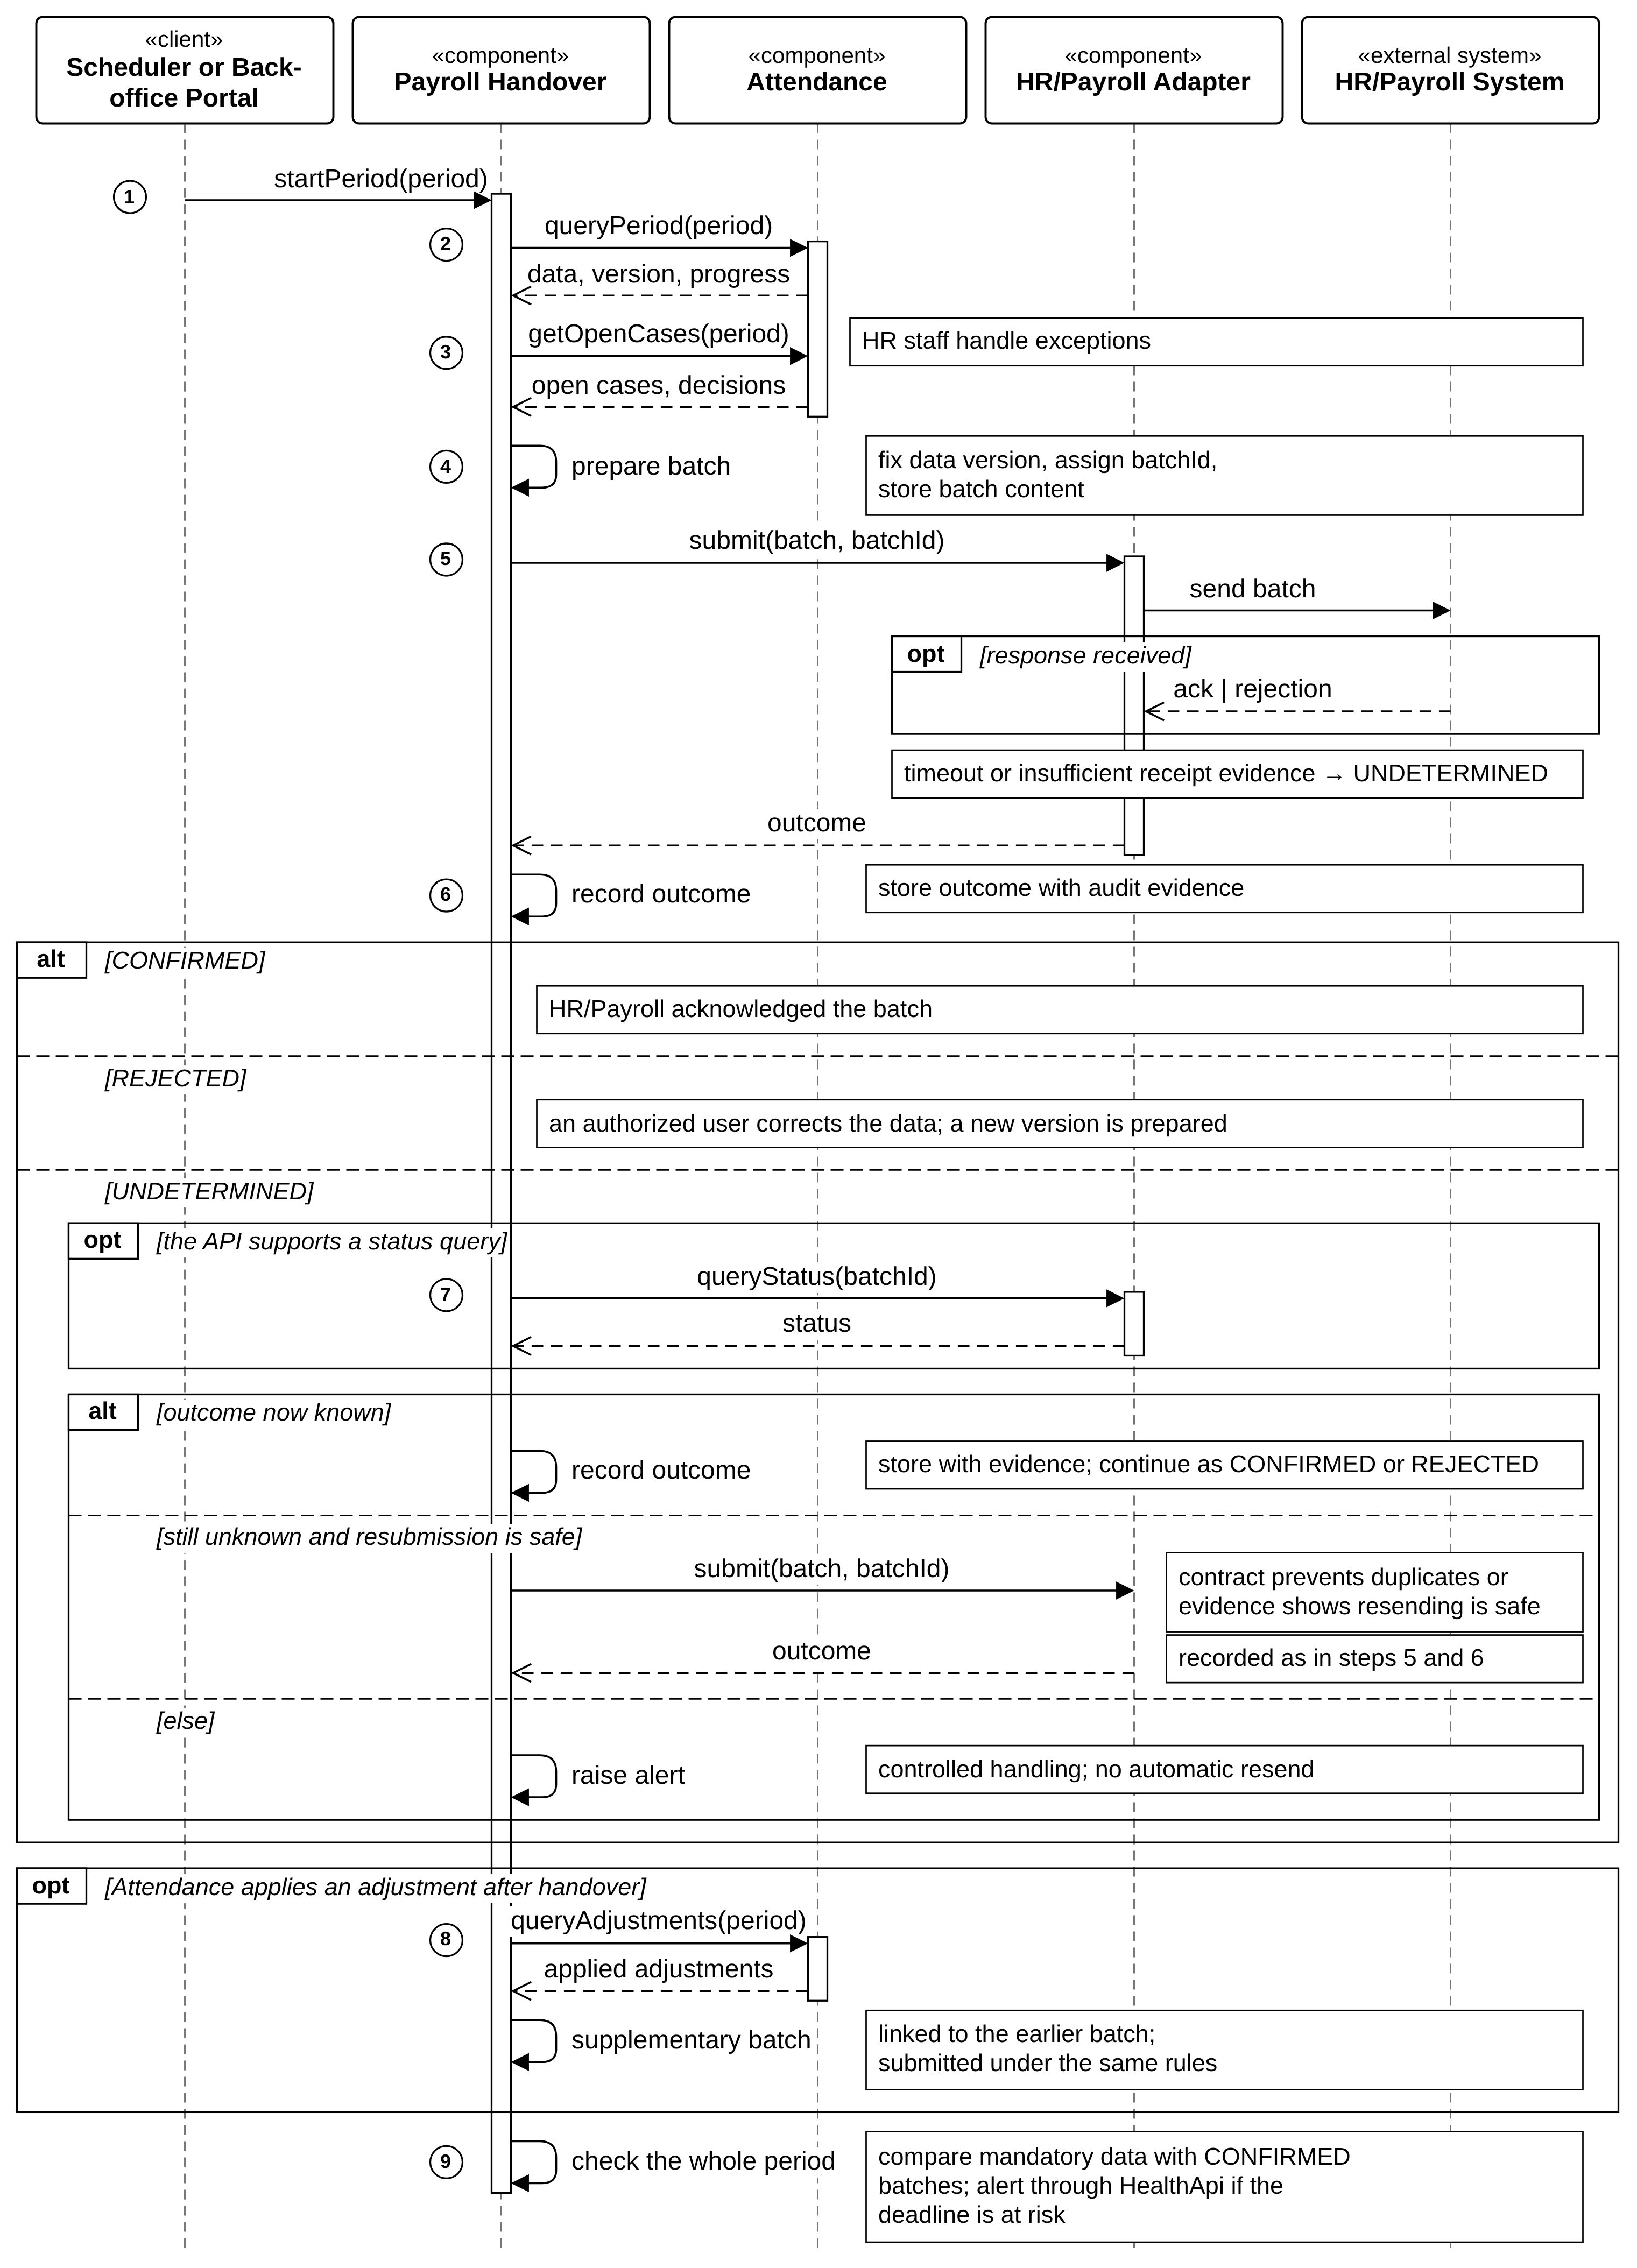
\includegraphics[width=450.0pt,height=630.0pt,keepaspectratio]{diagram/sequence/figure-4-17-payroll-handover.png}}{\fbox{\parbox{300pt}{\centering\vspace{20pt}Figure being redrawn\vspace{20pt}}}}
\par\vspace{4pt}
\textbf{Figure 4.17. Payroll Handover Sequence --- Preparation, Submission, Outcome and Supplementary Batch}\par
\phantomsection\addcontentsline{lof}{figure}{\protect\numberline{4.17}Payroll Handover Sequence --- Preparation, Submission, Outcome and Supplementary Batch}
\end{minipage}

\medskip


\Needspace{6\baselineskip}
The period follows these rules:

\begin{itemize}[leftmargin=36pt, itemsep=2pt, topsep=4pt, parsep=2pt]
  \item \textbf{Deadline (IC-01).} Data must be available at HR/Payroll before 12:00 noon on the first day of each month. We plan the first submission at 06:00 and an alert at 10:00 if the handover is still incomplete; these are checkpoints, not the final cutoff.
  \item \textbf{Shifts across a day or month.} Work Schedule Policy holds HR-approved rules for such shifts. Attendance Consolidation keeps the actual timestamps and uses these rules to assign transactions to a period. The month-end rule must be confirmed with HR before the first real handover.
  \item \textbf{Late records.} An overnight shift ending around 06:00 may not have its exit at the central site yet, so Payroll Handover checks expected shift completion, synchronization progress, and open cases before calling a period complete. It sends the available data at 06:00, marks the period incomplete, and sends later records in a linked supplementary batch, if possible before 12:00. If mandatory data is still missing at the deadline, the period stays incomplete, an alert is raised, and a later delivery is recorded as late.
  \item \textbf{Completion and deadline.} A batch acknowledgement only proves that HR/Payroll received that batch. A period is complete when all mandatory data has been handed over, and this is tracked separately from the deadline: a period can be complete but late, or on time but incomplete. Adjustments after a complete handover are not missing data.
  \item \textbf{Batch identity.} Resending unchanged content keeps its identifier and version under the contract; changed content gets a new identifier or version linked to the previous one. A batchId alone does not prove that resending is safe. A batch rejected for its content is corrected by an authorized user and sent as a new version.
\end{itemize}

\subsubsection*{4.2.5. States and Duplicate Prevention}

\phantomsection
\addcontentsline{toc}{subsubsection}{4.2.5. States and Duplicate Prevention}

The three flows rely on stored states and identifiers. NFR-02 covers only normal operation; component failures are assessed separately.

\Needspace{6\baselineskip}
Table 4.23a follows a scan up to the opening result, and Table 4.23b follows the passage and closing cycle, linked by scanId, commandId, and lane. OPEN\_CONFIRMED and CLOSED are command results; PASSAGE and LANE\_CLEAR are events. The table values are stored states. OPENED means that Gate Core has stored OPEN\_CONFIRMED.

\begin{longtable}{|>{\raggedright\arraybackslash}p{106.5pt}|>{\raggedright\arraybackslash}p{109.5pt}|>{\raggedright\arraybackslash}p{173.5pt}|}
\hline
\multicolumn{1}{|>{\columncolor{tableheader}\centering\arraybackslash}p{106.5pt}|}{\textbf{State}} & \multicolumn{1}{>{\columncolor{tableheader}\centering\arraybackslash}p{109.5pt}|}{\textbf{Meaning}} & \multicolumn{1}{>{\columncolor{tableheader}\centering\arraybackslash}p{173.5pt}|}{\textbf{Transition or Completion Conditions}} \\
\hline
\endhead
\multicolumn{3}{c}{\rule{0pt}{20pt}\normalsize\textbf{Table 4.23a. Scan States}} \\
\endlastfoot
RECEIVED & A new scan is being checked. & REJECTED if the checks fail, LANE BUSY if the lane is reserved, CANNOT PROCESS if something needed is missing, ACCEPTED if the checks pass and the atomic write succeeds. \\
\hline
LANE BUSY & The lane has an active or unresolved gate cycle. The token is not claimed. & End without a command; the employee scans again when the lane is free. \\
\hline
REJECTED & The QR code or access conditions are invalid, or the token is already claimed. & End without a command or attendance. \\
\hline
CANNOT PROCESS & Processing stopped before the command, for example because access data is unusable, ACCEPTED could not be stored, or the deadline passed before openGate. & No command is sent; the guard can start assisted access. \\
\hline
ACCEPTED & ACCEPTED is stored but there is no final outcome yet. This does not prove that no command was sent. & CANNOT PROCESS if the deadline expires before any command is sent; otherwise OPENED, CONTROLLER ERROR, or UNDETERMINED when the outcome is stored. Recover unfinished attempts from this state. \\
\hline
OPENED & The controller confirmed opening and the result is stored. This state alone does not establish passage or attendance. & Return the result to the kiosk. Missing passage after 15 seconds, or an emergency without passage evidence, leads to PENDING RECONCILIATION. \\
\hline
CONTROLLER ERROR & The controller explicitly confirmed that it did not open. & End without attendance; release the lane once the controller reports it ready. \\
\hline
UNDETERMINED & No reliable evidence of what the controller did. & Inquire if possible and move to the matching state; otherwise PENDING RECONCILIATION. Never resend the command to test. \\
\hline
PENDING RECONCILIATION & Not enough evidence for automatic attendance. & RECONCILED once Gate Core stores the authorized conclusion; earlier evidence is kept. \\*
\hline\noalign{\nobreak}
RECONCILED & Gate Core has stored the conclusion. & Send the acknowledgement; Attendance Review tracks the attendance change separately. \\
\hline
\end{longtable}
\phantomsection\addcontentsline{lot}{table}{\protect\numberline{4.23a}Scan States}


If the database cannot be written at all, RECEIVED and CANNOT PROCESS exist only as response states.

\Needspace{6\baselineskip}
Gate Core stores passageStatus and closureStatus separately, because the controller may end an opening opportunity before the 15-second passage observation ends. The observation timer starts at OPEN\_CONFIRMED and only flags a missing passage for review; it never permits closeGate.

\begin{longtable}{|>{\raggedright\arraybackslash}p{77pt}|>{\raggedright\arraybackslash}p{116pt}|>{\raggedright\arraybackslash}p{198pt}|}
\hline
\multicolumn{1}{|>{\columncolor{tableheader}\centering\arraybackslash}p{77pt}|}{\textbf{Track}} & \multicolumn{1}{>{\columncolor{tableheader}\centering\arraybackslash}p{116pt}|}{\textbf{Stored state}} & \multicolumn{1}{>{\columncolor{tableheader}\centering\arraybackslash}p{198pt}|}{\textbf{Transition and action}} \\
\hline
\endhead
\multicolumn{3}{c}{\rule{0pt}{20pt}\normalsize\textbf{Table 4.23b. Gate-Cycle States}} \\
\endlastfoot
Passage & WAITING & Set on OPEN\_CONFIRMED; wait for a PASSAGE event for this command and lane. \\
\hline
Passage & PASSED & For a timely, reliable QR passage while the scan is still OPENED, store the event and at most one original attendance transaction per scanId together. If already sent to reconciliation, for example by an emergency release, keep passage evidence for review without automatic attendance. Assisted cases still require HR approval. \\
\hline
Passage & NO\_PASSAGE & No reliable PASSAGE within 15 seconds; open a reconciliation case. A PASSAGE that arrives later is stored once with an audit record and marked LATE\_PASSAGE. It creates no attendance automatically; Attendance Review decides. It does not restart the 15-second timer or close the gate. \\
\hline
Closure & OPENED & Set on OPEN\_CONFIRMED; wait for LANE\_CLEAR. \\
\hline
Closure & CLEAR\_TO\_CLOSE & LANE\_CLEAR stored; one close command reserved. \\
\hline
Closure & CLOSE\_SENT & Persist closeCommandId before dispatch; the command may have been sent. Repeated events query that command rather than sending another. \\
\hline
Closure & CLOSED & Controller confirmed closing; the lane is released. Attendance is not affected. \\
\hline
Closure & CLOSE\_FAILED / CLOSE\_UNCERTAIN & Store the failure or unknown result and alert the guard; never claim CLOSED. The lane stays reserved until a query confirms CLOSED or a guard restores a safe state. \\*
\hline\noalign{\nobreak}
Emergency & EMERGENCY\_HOLD & Block normal closing and new scans on the lane until an authorized reset is confirmed, then follow the normal closing rule. \\
\hline
\end{longtable}
\phantomsection\addcontentsline{lot}{table}{\protect\numberline{4.23b}Gate-Cycle States}


\Needspace{6\baselineskip}
A few rules connect these states:

\begin{itemize}[leftmargin=36pt, itemsep=2pt, topsep=4pt, parsep=2pt]
  \item \textbf{Order.} Up to the stored opening result there is one sequence: check conditions; atomically reserve the lane, claim the token, and store ACCEPTED; send the opening command; store the outcome. Once the confirmed opening is stored, returning the kiosk result, recording passage, and closing safely run independently, each on its own signal: closing never waits for passage, and attendance never waits for closing or for the kiosk.
  \item \textbf{Timeouts.} If the station times out, it shows UNDETERMINED and calls getScanStatus with the same scanId instead of starting a new scan. Each request carries a deadline: Gate Transaction Processor does not start a command for an expired request, but it still checks a command that may already have been sent. If the deadline runs out after ACCEPTED but before openGate, nothing reached the controller, so the lane is released while the token stays claimed (Table 4.22).
  \item \textbf{History.} An approved adjustment is linked to the original scan and never overwrites it. Attendance Consolidation links an existing transaction or records a traceable adjustment instead of creating a second entry or exit, and late or conflicting passage evidence stays available for review.
  \item \textbf{No reliable PASSAGE signal.} The I-07 rule cannot run. An independent passage sensor must be verified first; until then, attendance comes from evidenced assisted records approved by HR.
  \item \textbf{Recovery.} Gate Transaction Processor reviews uncertain openings and OPENED scans awaiting passage or closure, queries the controller where supported, and otherwise sends the case to reconciliation or alerts the guard as in Table 4.22. Site Sync redelivers unacknowledged events with their original identifiers. Access Decision uses Eligibility Snapshot only under the version, continuity, and freshness conditions of degraded mode (I-10), and marks each degraded decision for review after reconnection.
\end{itemize}

\Needspace{6\baselineskip}
Table 4.24 lists the identifiers that keep scans, commands, events, and batches apart. A scan can produce several events, and a redelivered event keeps its eventId.

\begin{longtable}{|>{\raggedright\arraybackslash}p{95pt}|>{\raggedright\arraybackslash}p{120pt}|>{\raggedright\arraybackslash}p{190pt}|}
\hline
\multicolumn{1}{|>{\columncolor{tableheader}\centering\arraybackslash}p{95pt}|}{\textbf{Identifier}} & \multicolumn{1}{>{\columncolor{tableheader}\centering\arraybackslash}p{120pt}|}{\textbf{Owner}} & \multicolumn{1}{>{\columncolor{tableheader}\centering\arraybackslash}p{190pt}|}{\textbf{Use}} \\
\hline
\endhead
\multicolumn{3}{c}{\rule{0pt}{20pt}\normalsize\textbf{Table 4.24. Identifiers Used across the Main Flows}} \\
\endlastfoot
scanId & Station Client & One scan and its status inquiries. \\
\hline
commandId & Gate Transaction Processor & Links each opening or closing command to its result; it does not by itself prevent duplicate execution. \\
\hline
passageEventId & Turnstile controller & Stable identifier for a passage event, linked to the lane and opening command under I-01. \\
\hline
tokenId & QR Credential Issuance & Identifies a QR code under the proposed single-use policy. \\
\hline
eventId & Event producer & Identifies a transferred event and remains the same on retry. \\
\hline
Version or sequence & Owning data source & Detects missing or out-of-order updates. \\
\hline
supportCaseId & Gate Intervention & Links an assistance case to its evidence and scan, when present. \\
\hline
Decision ID and version & Attendance Review & Tracks approval and safe repeated application. \\*
\hline\noalign{\nobreak}
batchId and version & Payroll Handover & Tracks a handover, retry, or supplementary batch. \\
\hline
\end{longtable}
\phantomsection\addcontentsline{lot}{table}{\protect\numberline{4.24}Identifiers Used across the Main Flows}


\Needspace{6\baselineskip}
The identifiers prevent three kinds of duplicates:

\begin{itemize}[leftmargin=36pt, itemsep=2pt, topsep=4pt, parsep=2pt]
  \item \textbf{Duplicate events.} Each receiver stores the business change and an event-processed marker together, and returns the stored outcome when the same event arrives again.
  \item \textbf{Duplicate attendance.} Gate Transaction Processor accepts each passageEventId once and creates at most one original QR transaction per scanId; a second, different passage is kept as an anomaly. Attendance Consolidation checks the scan link again when it receives transactions or applies decisions.
  \item \textbf{QR replay.} The token is claimed in the same atomic write as ACCEPTED; Access Decision only verifies it. A unique-token constraint only works within the store that enforces it, and finding a duplicate after the gate has opened is only anomaly detection.
\end{itemize}

\Needspace{6\baselineskip}
Table 4.25 lists the handover batch states used in Flow C.

\begin{longtable}{|>{\raggedright\arraybackslash}p{108.5pt}|>{\raggedright\arraybackslash}p{129.5pt}|>{\raggedright\arraybackslash}p{171.5pt}|}
\hline
\multicolumn{1}{|>{\columncolor{tableheader}\centering\arraybackslash}p{108.5pt}|}{\textbf{State}} & \multicolumn{1}{>{\columncolor{tableheader}\centering\arraybackslash}p{129.5pt}|}{\textbf{Meaning}} & \multicolumn{1}{>{\columncolor{tableheader}\centering\arraybackslash}p{171.5pt}|}{\textbf{Handling}} \\
\hline
\endhead
\multicolumn{3}{c}{\rule{0pt}{20pt}\normalsize\textbf{Table 4.25. Handover Batch States}} \\
\endlastfoot
PREPARED & Batch content and identity have been stored. & Submit through HR/Payroll Adapter. \\
\hline
SENT & A submission has occurred; the outcome is being determined. & Track acknowledgements or errors. \\
\hline
CONFIRMED & Receipt evidence that satisfies I-02. & Store the acknowledgement and update period progress. \\
\hline
REJECTED & HR/Payroll clearly refused the content. & Handle within authority and create a new version. \\*
\hline\noalign{\nobreak}
UNDETERMINED & A timeout, or a response without enough receipt evidence. & Inquire, resubmit when safe, or route for controlled handling. \\
\hline
\end{longtable}
\phantomsection\addcontentsline{lot}{table}{\protect\numberline{4.25}Handover Batch States}


\Needspace{9\baselineskip}
\subsection*{4.3. Class Responsibilities for the Gate Flow}

\phantomsection
\addcontentsline{toc}{subsection}{4.3. Class Responsibilities for the Gate Flow}


The proposed classes for the gate flow keep the scan, the controller command, the gate cycle, the passage evidence, and the attendance transaction apart:

\begin{itemize}[leftmargin=36pt, itemsep=2pt, topsep=4pt, parsep=2pt]
  \item \textbf{StationClient} submits a scan through GateCoreApi.
  \item \textbf{GateTransactionProcessor} checks the existing ScanAttempt, asks AccessDecision to evaluate the QR code against EligibilitySnapshot, and stores the ACCEPTED attempt, its TokenReservation, and a new GateCycle for the lane in one transaction before calling the controller port.
  \item \textbf{GateCommand} carries a commandId linked to its scan or support case and lane.
  \item The \textbf{TurnstileAdapter} class implements the turnstile command ports (IOpenGate, ICloseGate, IEmergencyGate) and reports PASSAGE and LANE\_CLEAR through IPassageEvents. A receipt stays internal to the adapter. For openGate, the final outcome is OPEN\_CONFIRMED, CONTROLLER ERROR (confirmed non-execution), or UNDETERMINED.
  \item \textbf{GateCycle} holds the passage and closure states, the 15-second observation deadline, the lane-clear signal, and the close command. While a lane has an active or unresolved GateCycle, the lane is busy.
  \item \textbf{PassageEvent} is stored before \textbf{AttendanceTransaction} is created. The data model allows at most one original transaction per scanId and accepts each passageEventId once.
\end{itemize}

The class diagrams below are drawn from the Task 2 code (Chapter 9), so the names are the ones in \code{src/tmc_gate}. In all three figures a solid arrow means that a class uses another one, a dashed arrow with a hollow triangle means that it implements an interface, a solid line with a hollow triangle means that an interface extends another one, and interface names are in italics. Only the operations needed to follow the flow are shown.

\Needspace{12\baselineskip}
\subsubsection*{4.3.1. Scan Flow}

\phantomsection
\addcontentsline{toc}{subsubsection}{4.3.1. Scan Flow}

\noindent\begin{minipage}{\linewidth}
\centering
\IfFileExists{diagram/class/figure-4-18-scan-flow-classes.png}{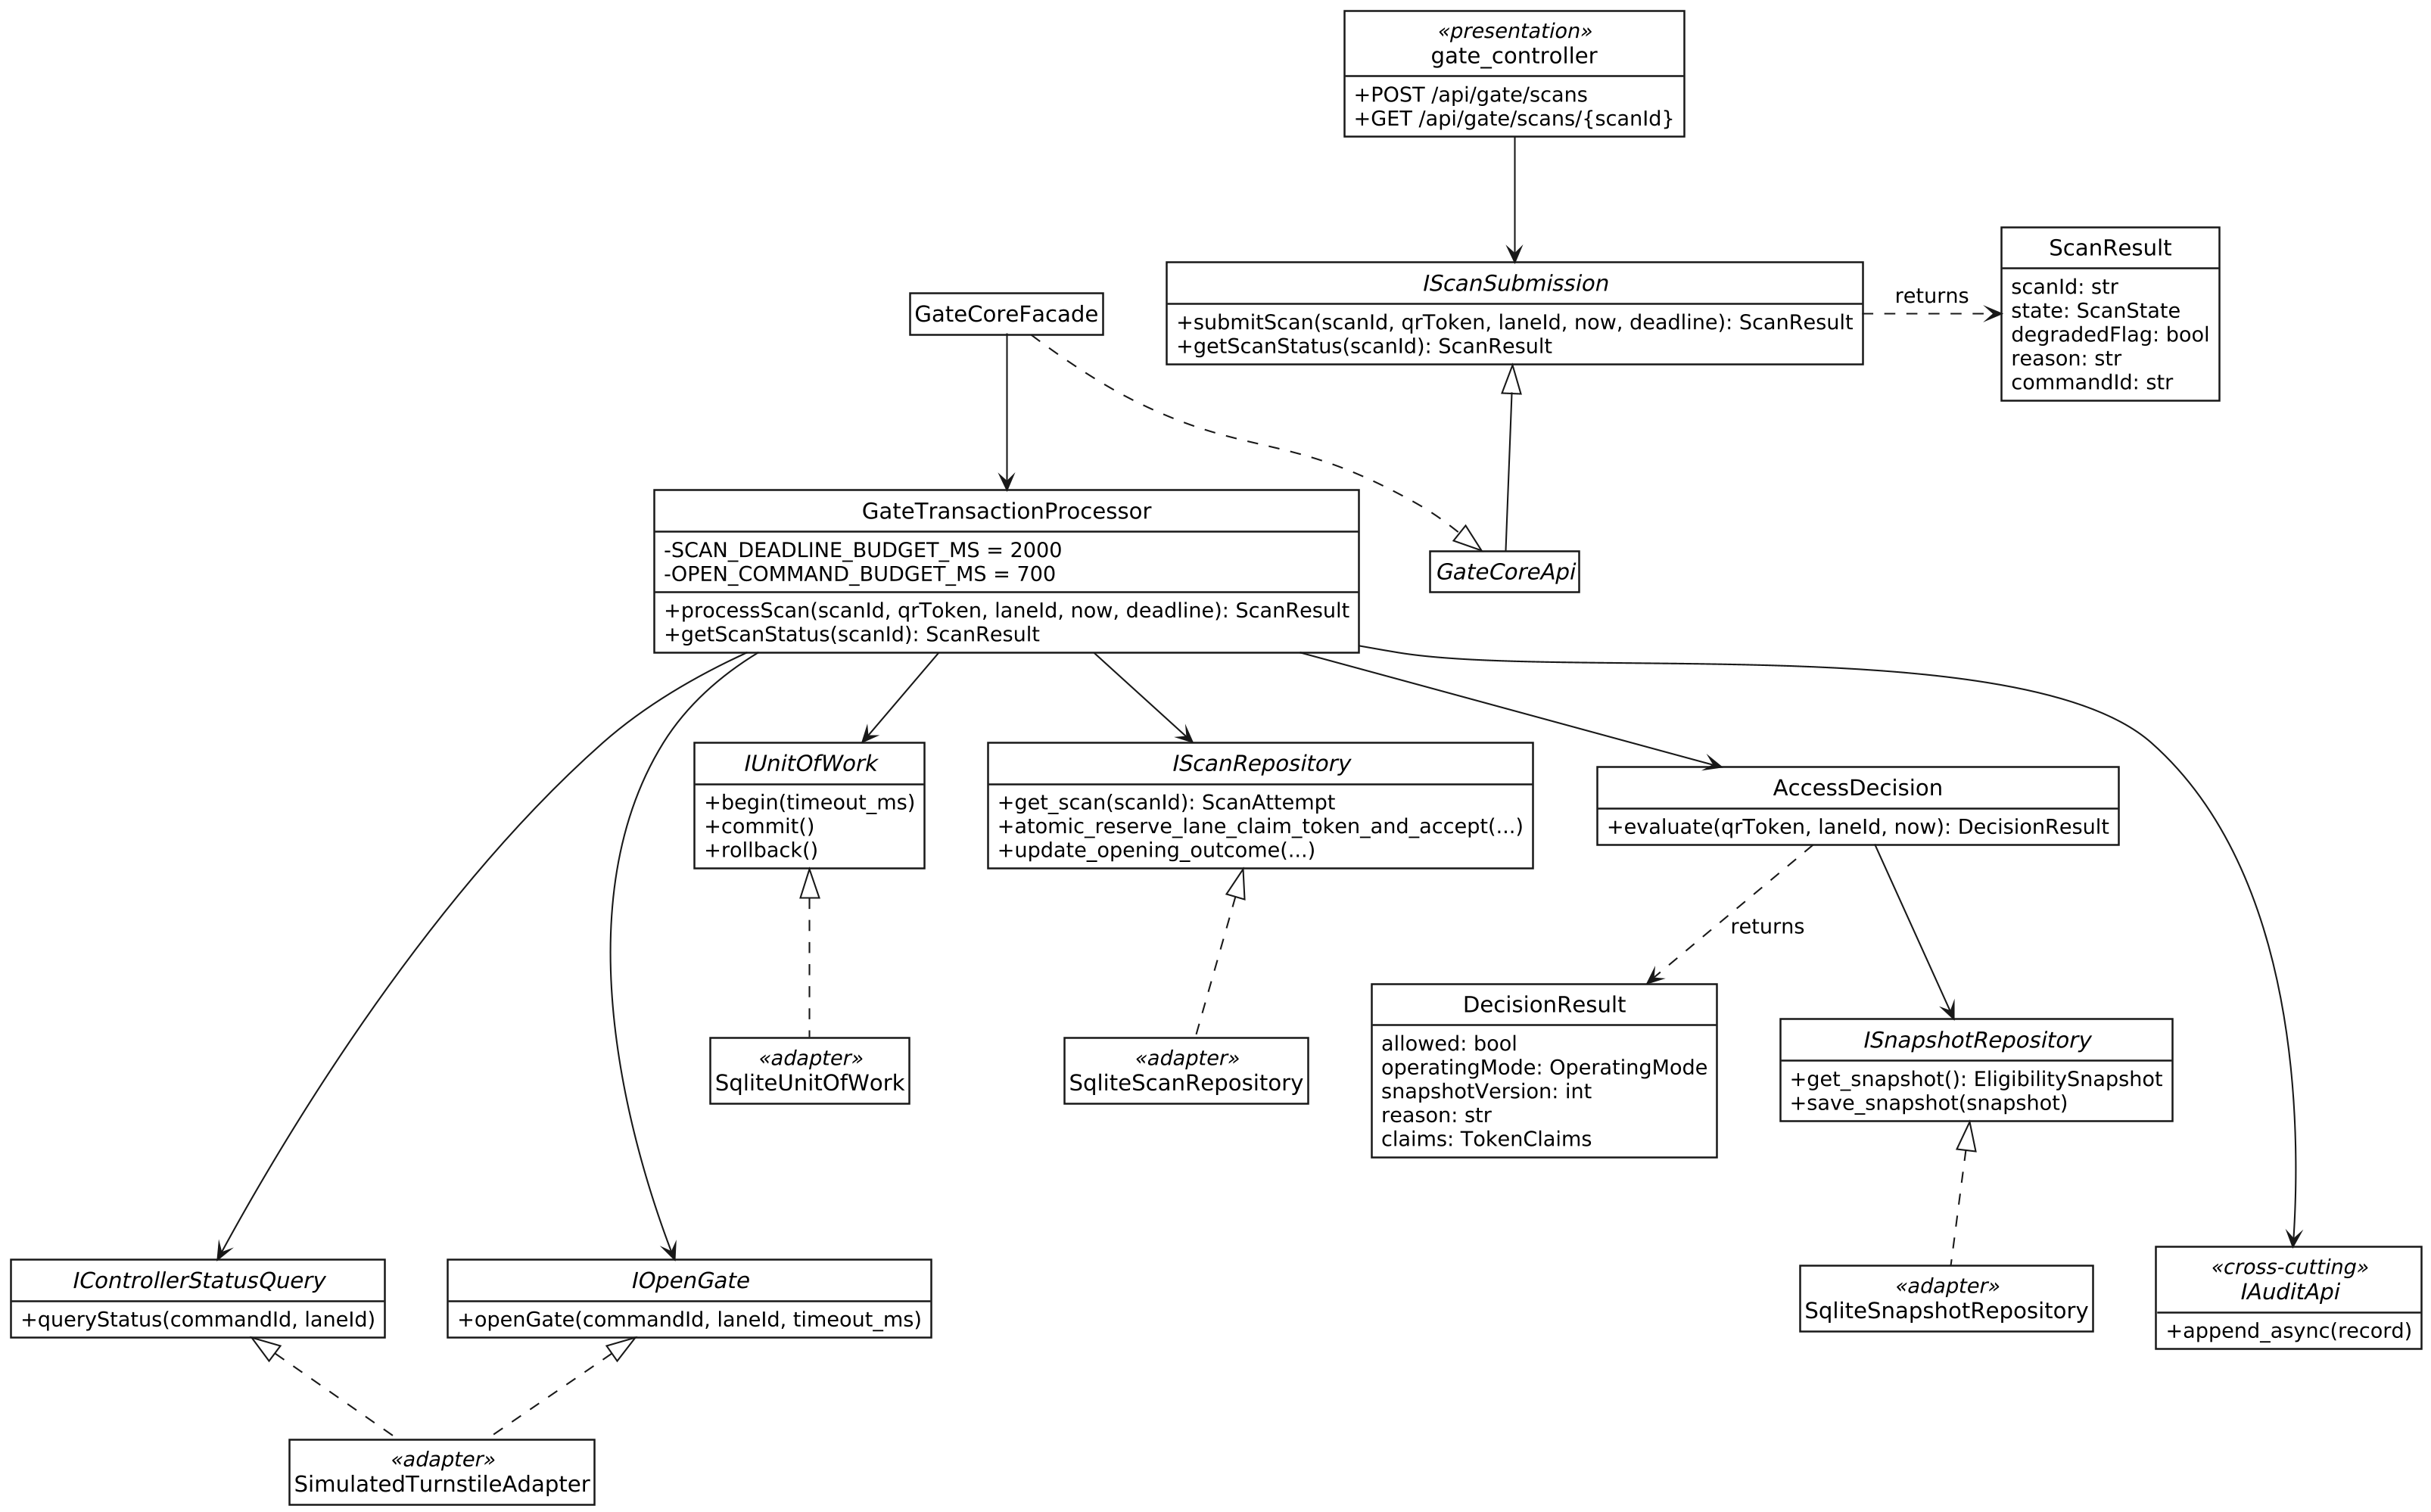
\includegraphics[width=\linewidth,height=330pt,keepaspectratio]{diagram/class/figure-4-18-scan-flow-classes.png}}{\fbox{\parbox{300pt}{\centering\vspace{20pt}Figure being redrawn\vspace{20pt}}}}

\vspace{6pt}
\textbf{Figure 4.18. Class Diagram of the Scan Flow}
\phantomsection\addcontentsline{lof}{figure}{\protect\numberline{4.18}Class Diagram of the Scan Flow}
\end{minipage}

\vspace{10pt}

Figure 4.18 shows the classes behind a QR scan (Flow A). The kiosk route in the \code{gate_controller} router only knows IScanSubmission. GateCoreFacade implements it through GateCoreApi and hands the scan to GateTransactionProcessor, which is the only class that coordinates the flow. The processor asks AccessDecision for the decision, and AccessDecision reads the EligibilitySnapshot through ISnapshotRepository. Every other dependency of the processor is an interface: IScanRepository and IUnitOfWork for the transaction, IOpenGate and IControllerStatusQuery for the controller, and IAuditApi for audit evidence. All of them are passed in through the constructor in \code{app.py}.

The two budgets in the processor come from Table 5.5: the whole scan must finish within 2 seconds, and openGate gets at most 700 ms of that time. The processor stores the ACCEPTED scan, its TokenReservation, and the new GateCycle in one transaction before it sends openGate, so a crash after the command still leaves evidence that the lane is taken.

\Needspace{12\baselineskip}
\subsubsection*{4.3.2. Controller Signals and Gate Intervention}

\phantomsection
\addcontentsline{toc}{subsubsection}{4.3.2. Controller Signals and Gate Intervention}

\noindent\begin{minipage}{\linewidth}
\centering
\IfFileExists{diagram/class/figure-4-19-signals-intervention-classes.png}{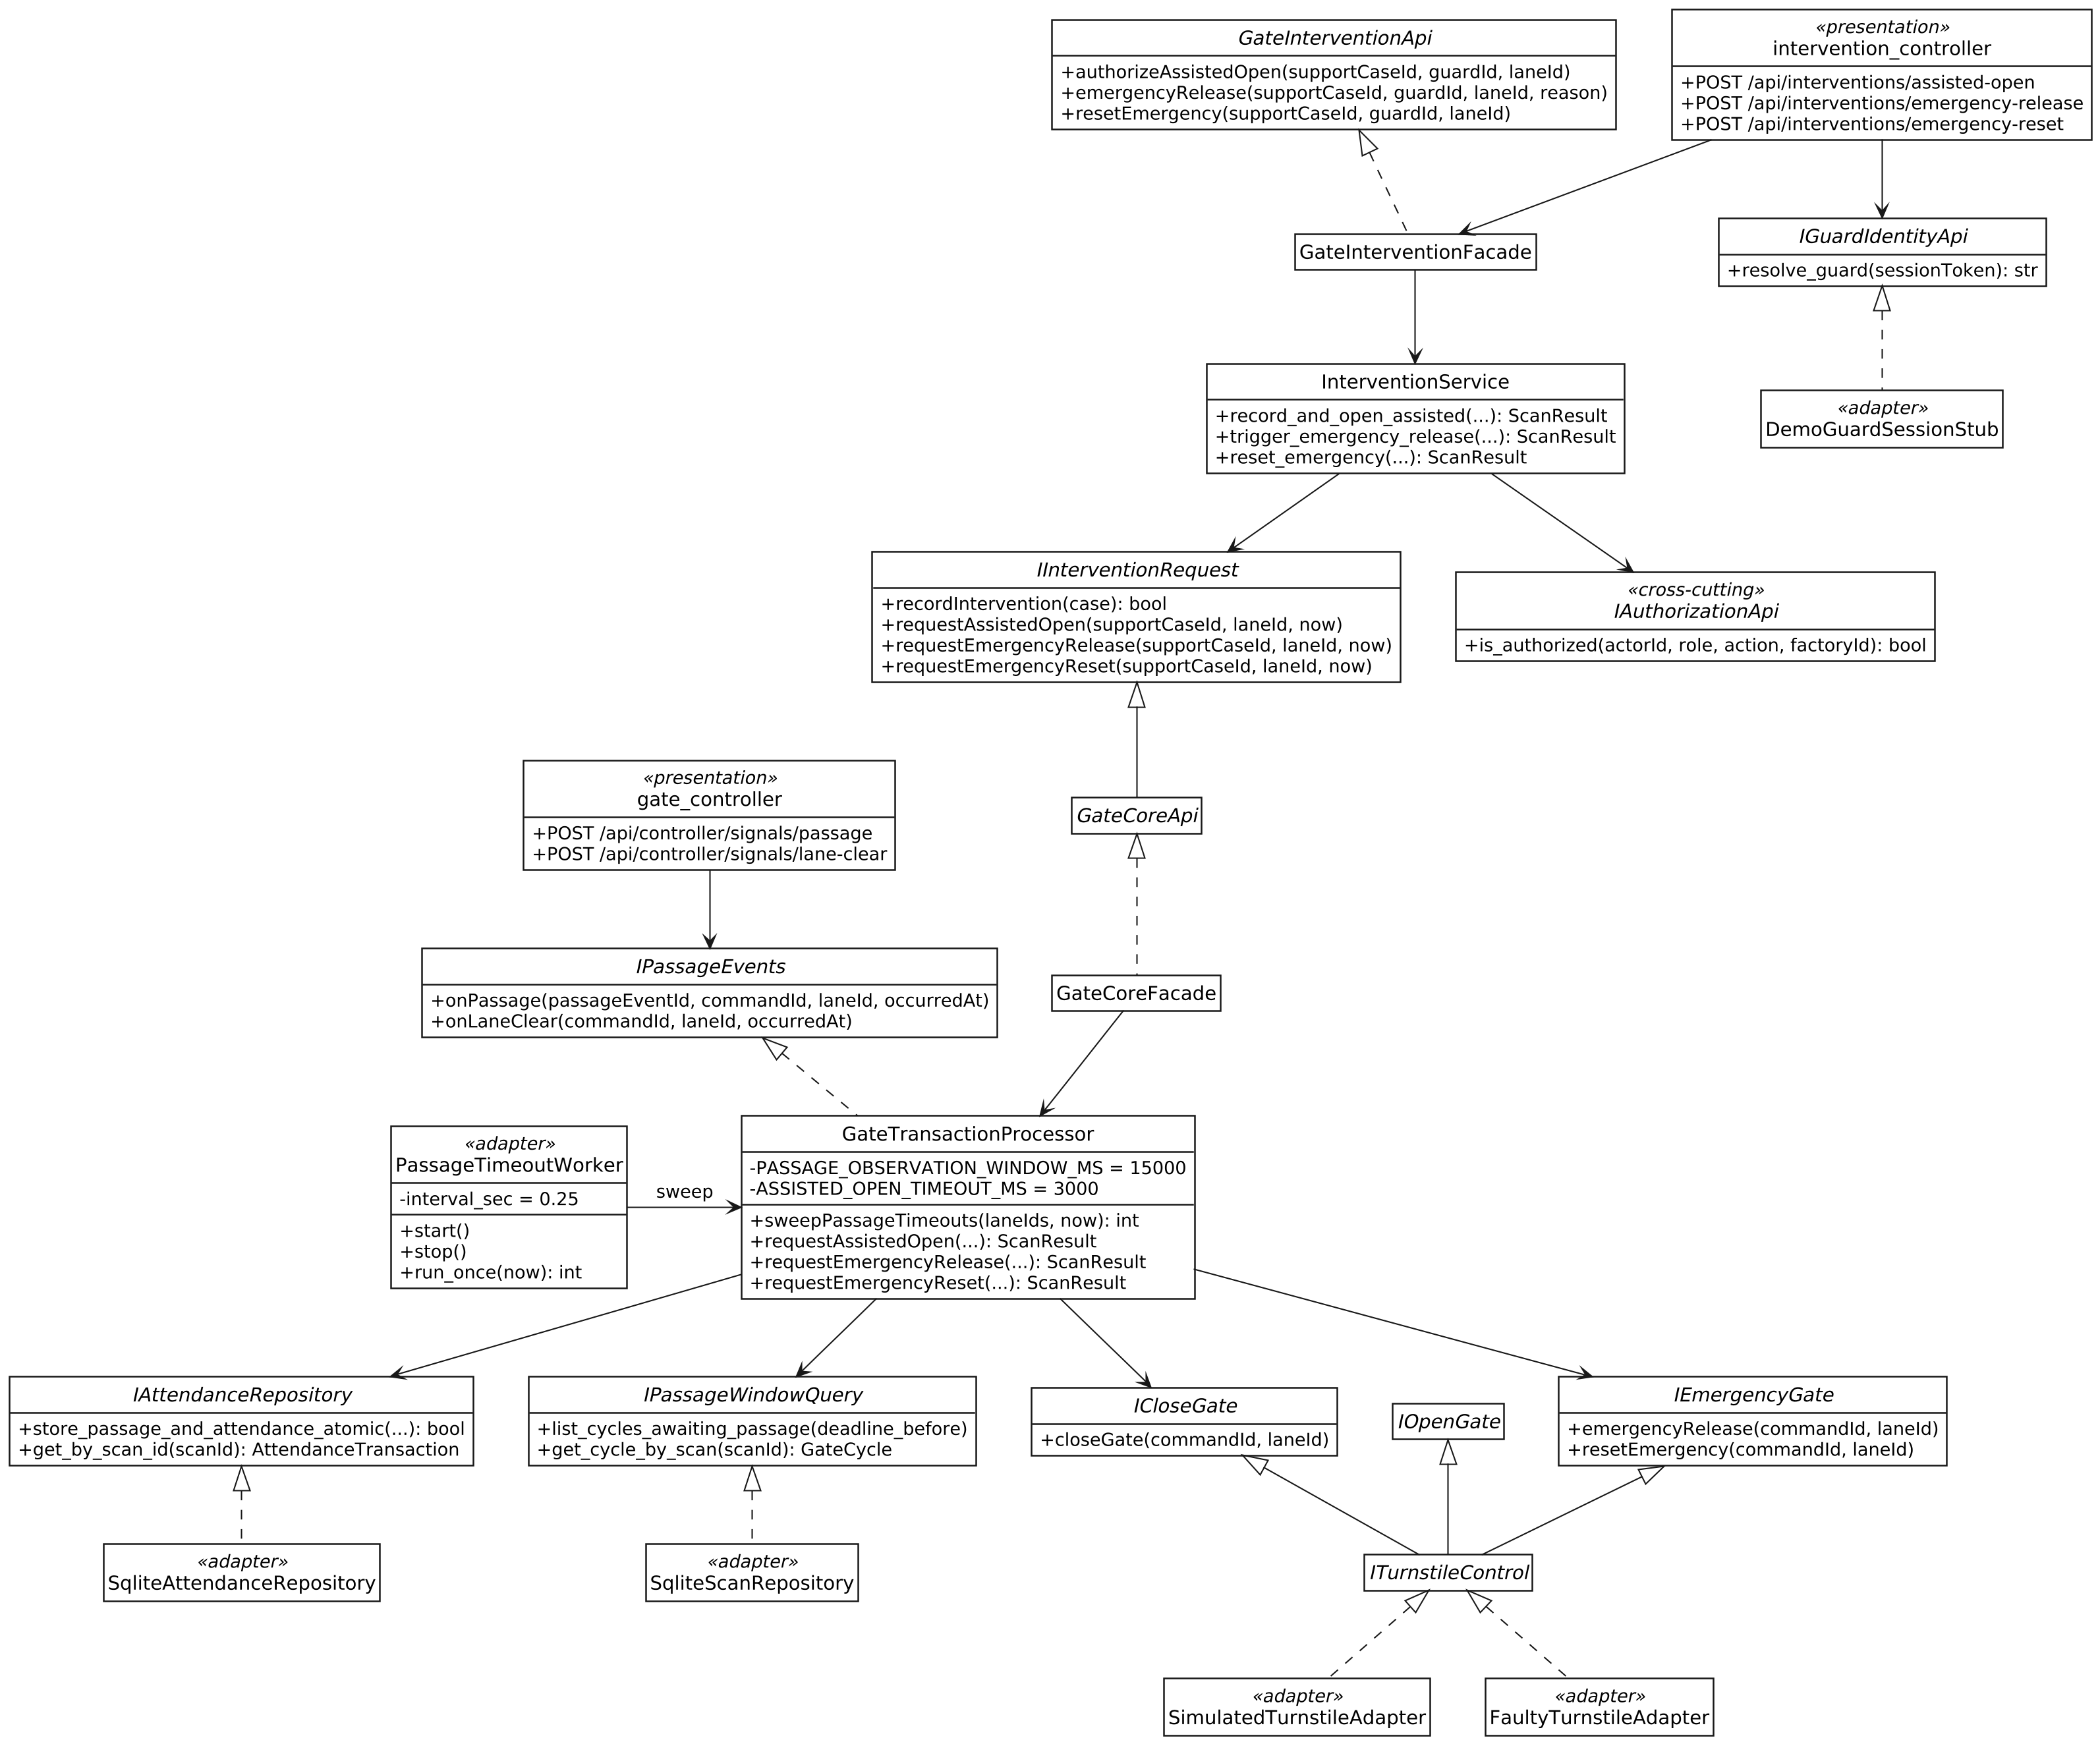
\includegraphics[width=\linewidth,height=420pt,keepaspectratio]{diagram/class/figure-4-19-signals-intervention-classes.png}}{\fbox{\parbox{300pt}{\centering\vspace{20pt}Figure being redrawn\vspace{20pt}}}}

\vspace{6pt}
\textbf{Figure 4.19. Class Diagram of Controller Signals and Gate Intervention}
\phantomsection\addcontentsline{lof}{figure}{\protect\numberline{4.19}Class Diagram of Controller Signals and Gate Intervention}
\end{minipage}

\vspace{10pt}

Figure 4.19 shows the other ways into Gate Core. PASSAGE and LANE\_CLEAR from the controller arrive at \code{gate_controller} and go to GateTransactionProcessor through IPassageEvents. PassageTimeoutWorker calls sweepPassageTimeouts every 0.25 seconds. The processor then uses IPassageWindowQuery to find the cycles whose 15-second window has ended. This timer never sends closeGate.

Guard actions (Flow B) take a separate path. \code{intervention_controller} gets the guard from the session through IGuardIdentityApi, and InterventionService checks the guard's authority through IAuthorizationApi before it calls Gate Core. InterventionService only sees IInterventionRequest, not the whole GateCoreApi, which is the ISP split of Section 7.1. The turnstile ports are also split: one adapter class implements ITurnstileControl, but the processor depends on IOpenGate, ICloseGate, and IEmergencyGate one by one. FaultyTurnstileAdapter is a second implementation that the contract tests use to check the LSP rule (Section 9.4).

\Needspace{12\baselineskip}
\subsubsection*{4.3.3. Gate Core Entities}

\phantomsection
\addcontentsline{toc}{subsubsection}{4.3.3. Gate Core Entities}

\noindent\begin{minipage}{\linewidth}
\centering
\IfFileExists{diagram/class/figure-4-20-gate-core-entities.png}{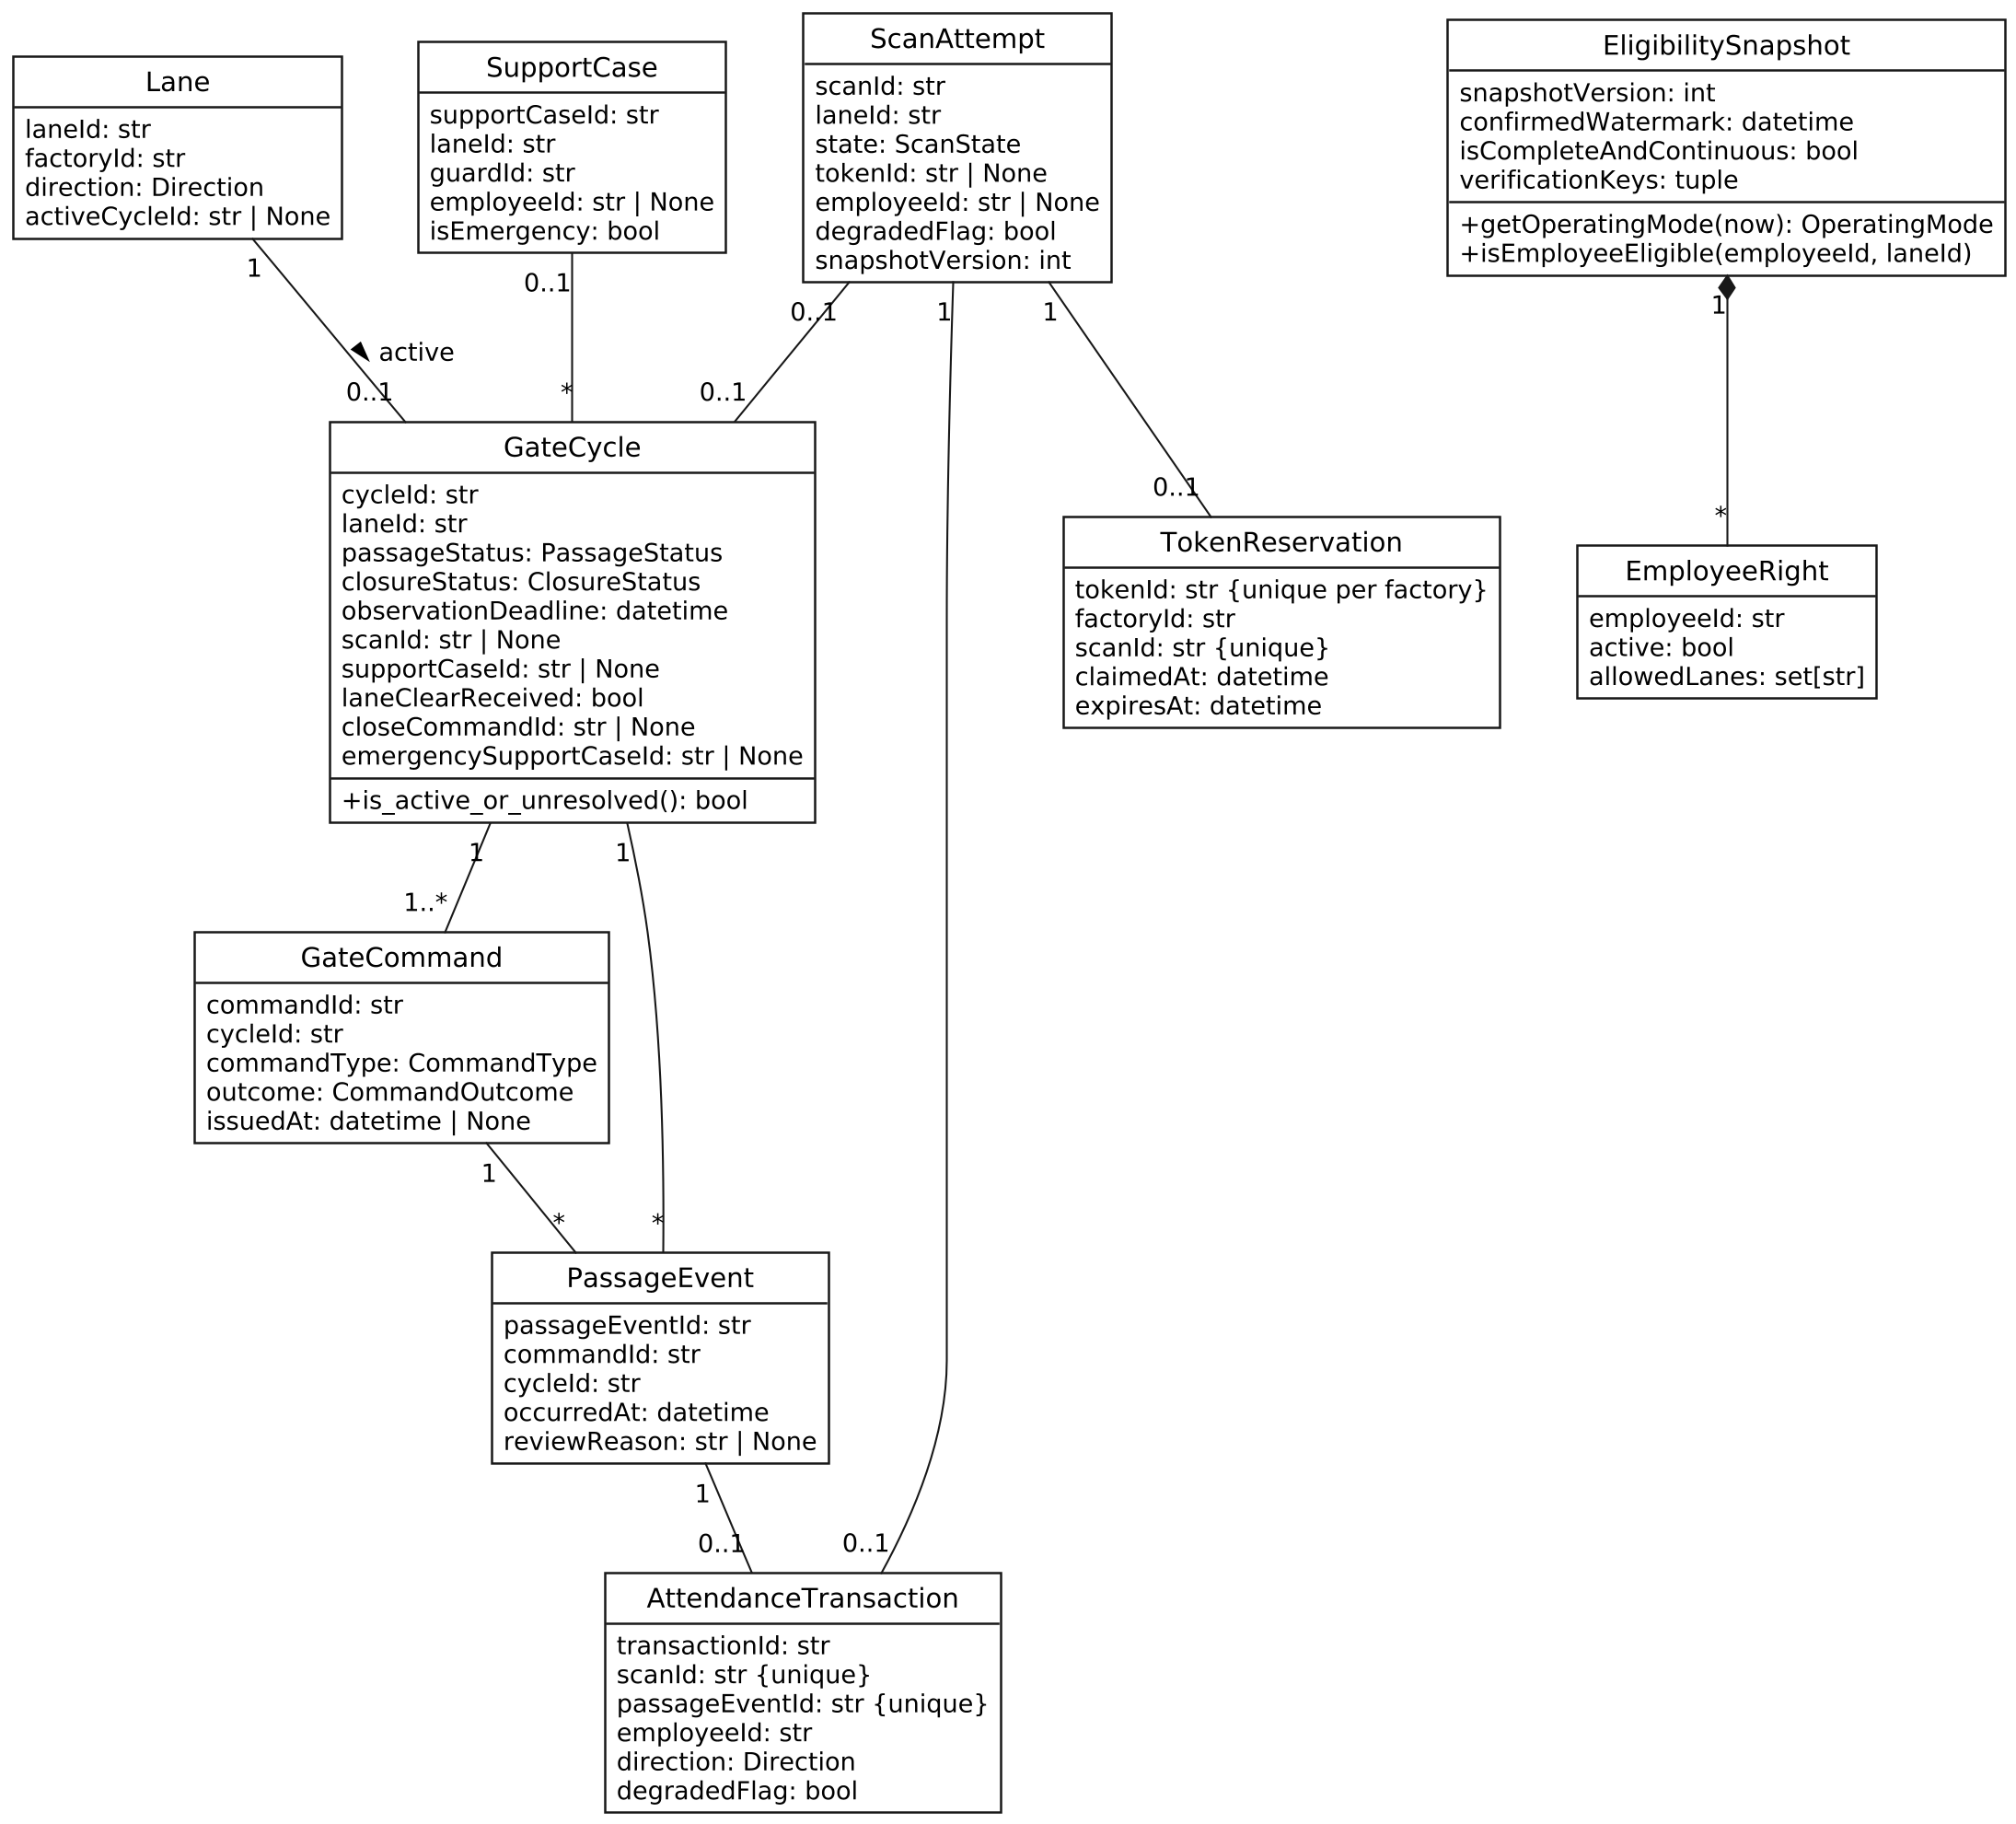
\includegraphics[width=\linewidth,height=420pt,keepaspectratio]{diagram/class/figure-4-20-gate-core-entities.png}}{\fbox{\parbox{300pt}{\centering\vspace{20pt}Figure being redrawn\vspace{20pt}}}}

\vspace{6pt}
\textbf{Figure 4.20. Gate Core Entities and Their Multiplicities}
\phantomsection\addcontentsline{lof}{figure}{\protect\numberline{4.20}Gate Core Entities and Their Multiplicities}
\end{minipage}

\vspace{10pt}

Figure 4.20 shows the entities and their multiplicities, including the rule that a Lane has at most one active GateCycle. A later close failure never erases a confirmed attendance transaction, and neither assisted nor emergency opening creates attendance from the opening alone.

Table 4.26 lists the enumerations that appear as attribute types in Figures 4.18 to 4.20. The values are the ones in \code{src/tmc_gate/domain/enums.py}.

\begin{longtable}{|>{\raggedright\arraybackslash}p{92pt}|>{\raggedright\arraybackslash}p{178pt}|>{\raggedright\arraybackslash}p{141pt}|}
\hline
\multicolumn{1}{|>{\columncolor{tableheader}\centering\arraybackslash}p{92pt}|}{\textbf{Type}} & \multicolumn{1}{>{\columncolor{tableheader}\centering\arraybackslash}p{178pt}|}{\textbf{Values}} & \multicolumn{1}{>{\columncolor{tableheader}\centering\arraybackslash}p{141pt}|}{\textbf{Used in}} \\
\hline
\endhead
\multicolumn{3}{c}{\rule{0pt}{20pt}\normalsize\phantomsection\addcontentsline{lot}{table}{\protect\numberline{4.26}Value Types Used in the Class Diagrams}\textbf{Table 4.26. Value Types Used in the Class Diagrams}} \\
\endlastfoot
ScanState & RECEIVED, ACCEPTED, OPENED, REJECTED, LANE\_BUSY, CANNOT\_PROCESS, CONTROLLER\_ERROR, UNDETERMINED, PENDING\_RECONCILIATION, RECONCILED & \code{ScanAttempt.state} \\
\hline
PassageStatus & WAITING, PASSED, NO\_PASSAGE & \code{GateCycle.passageStatus} \\
\hline
ClosureStatus & OPENED, CLEAR\_TO\_CLOSE, CLOSE\_SENT, CLOSED, CLOSE\_FAILED, CLOSE\_UNCERTAIN, EMERGENCY\_HOLD & \code{GateCycle.closureStatus} \\
\hline
CommandType & OPEN, CLOSE, EMERGENCY\_RELEASE, RESET & \code{GateCommand.commandType} \\
\hline
CommandOutcome & SENT, NOT\_SENT, OPEN\_CONFIRMED, CLOSED, EMERGENCY\_RELEASED, RESET\_CONFIRMED, CONTROLLER\_ERROR, UNDETERMINED & \code{GateCommand.outcome}; SENT and NOT\_SENT are stored states only, a port never returns them \\
\hline
OperatingMode & NORMAL, DEGRADED, CANNOT\_PROCESS & Result of \code{EligibilitySnapshot.getOperatingMode} (Figure 5.3) \\*
\hline\noalign{\nobreak}
Direction & ENTRY, EXIT & direction of Lane and of AttendanceTransaction \\
\hline
\end{longtable}


\newpage
% ==================== CHAPTER 5 ====================
\section*{5. PHYSICAL ARCHITECTURE}

\phantomsection
\addcontentsline{toc}{section}{5. PHYSICAL ARCHITECTURE}

This chapter shows where the components of Chapter 4 run, how the nodes are connected, how data is kept, and what happens when parts of the system fail. Gate processing runs at each of the two factories, and management functions run at the central site. Each factory has its own application and database, stores its transactions locally, and sends them to the central site later. Access rights and configuration are managed centrally and sent to the factories.

\Needspace{6\baselineskip}
The deployment covers the Binh Duong and Long An factories, the TMC central site, and the existing external systems: the turnstile controllers, HR/Payroll, and TMC's email service. We use the following proposals and assumptions; TMC has to confirm them before deployment:

\begin{itemize}[leftmargin=36pt, itemsep=2pt, topsep=4pt, parsep=2pt]
  \item \textbf{Factory servers.} Each factory has a server environment for the factory application and its local database, with a standby on separate resources, so that one failure cannot stop both. Factory Monitoring runs inside the factory application. The two factories never share a database for the QR flow.
  \item \textbf{Central site.} It runs the central application, its database, the message broker, the reverse proxy, and central Monitoring.
  \item \textbf{Network.} Factories connect to the central site over a private network or VPN. APIs and messaging channels use encryption and component authentication.
  \item \textbf{Lanes.} Each lane has one kiosk and one controller. The number of lanes, server sizes, and storage capacity come from the site survey; we do not assume four lanes per factory.
  \item \textbf{Infrastructure services.} Time synchronization, backup, and key management come from the infrastructure and do not take over the responsibilities of business components.
  \item \textbf{External systems.} We assume the controller signals in I-01 and I-05 and the HR/Payroll acknowledgement in I-02. These signals, the controller protocol, and where HR/Payroll physically runs must be confirmed with their operators. Placing HR/Payroll in an integration zone in the diagram does not mean that TMC has to move it.
\end{itemize}

\Needspace{6\baselineskip}
We built the physical architecture in four steps:

\begin{itemize}[leftmargin=46pt, labelwidth=40pt, labelsep=6pt, align=left, itemsep=3pt, topsep=4pt, parsep=2pt]
  \item[\textbf{Step 1}] \textbf{Place the work.} Gate work goes to each factory and office work to the central site, following the quanta in Chapter 3 (Section 5.1).
  \item[\textbf{Step 2}] \textbf{Choose nodes and redundancy.} Each application gets the nodes it needs, with a standby only where availability requires it (Section 5.2).
  \item[\textbf{Step 3}] \textbf{Map components and connections.} Every component from Chapter 4 is placed on a node, and every link gets a protocol and a security boundary (Sections 5.2, 5.3, and 5.5).
  \item[\textbf{Step 4}] \textbf{Check quality and failures.} The 2-second budget, data persistence, and the behavior under each failure are checked against the driving characteristics (Sections 5.4, 5.6, and 5.7).
\end{itemize}


\clearpage
\subsection*{5.1. Deployment Diagram}

\phantomsection
\addcontentsline{toc}{subsection}{5.1. Deployment Diagram}

Figure 5.1 is the allocation view of TMC across the two factories, the central site, and the external systems.

\noindent\begin{minipage}{\linewidth}
\centering
\IfFileExists{diagram/deployment/figure-5-1-deployment.png}{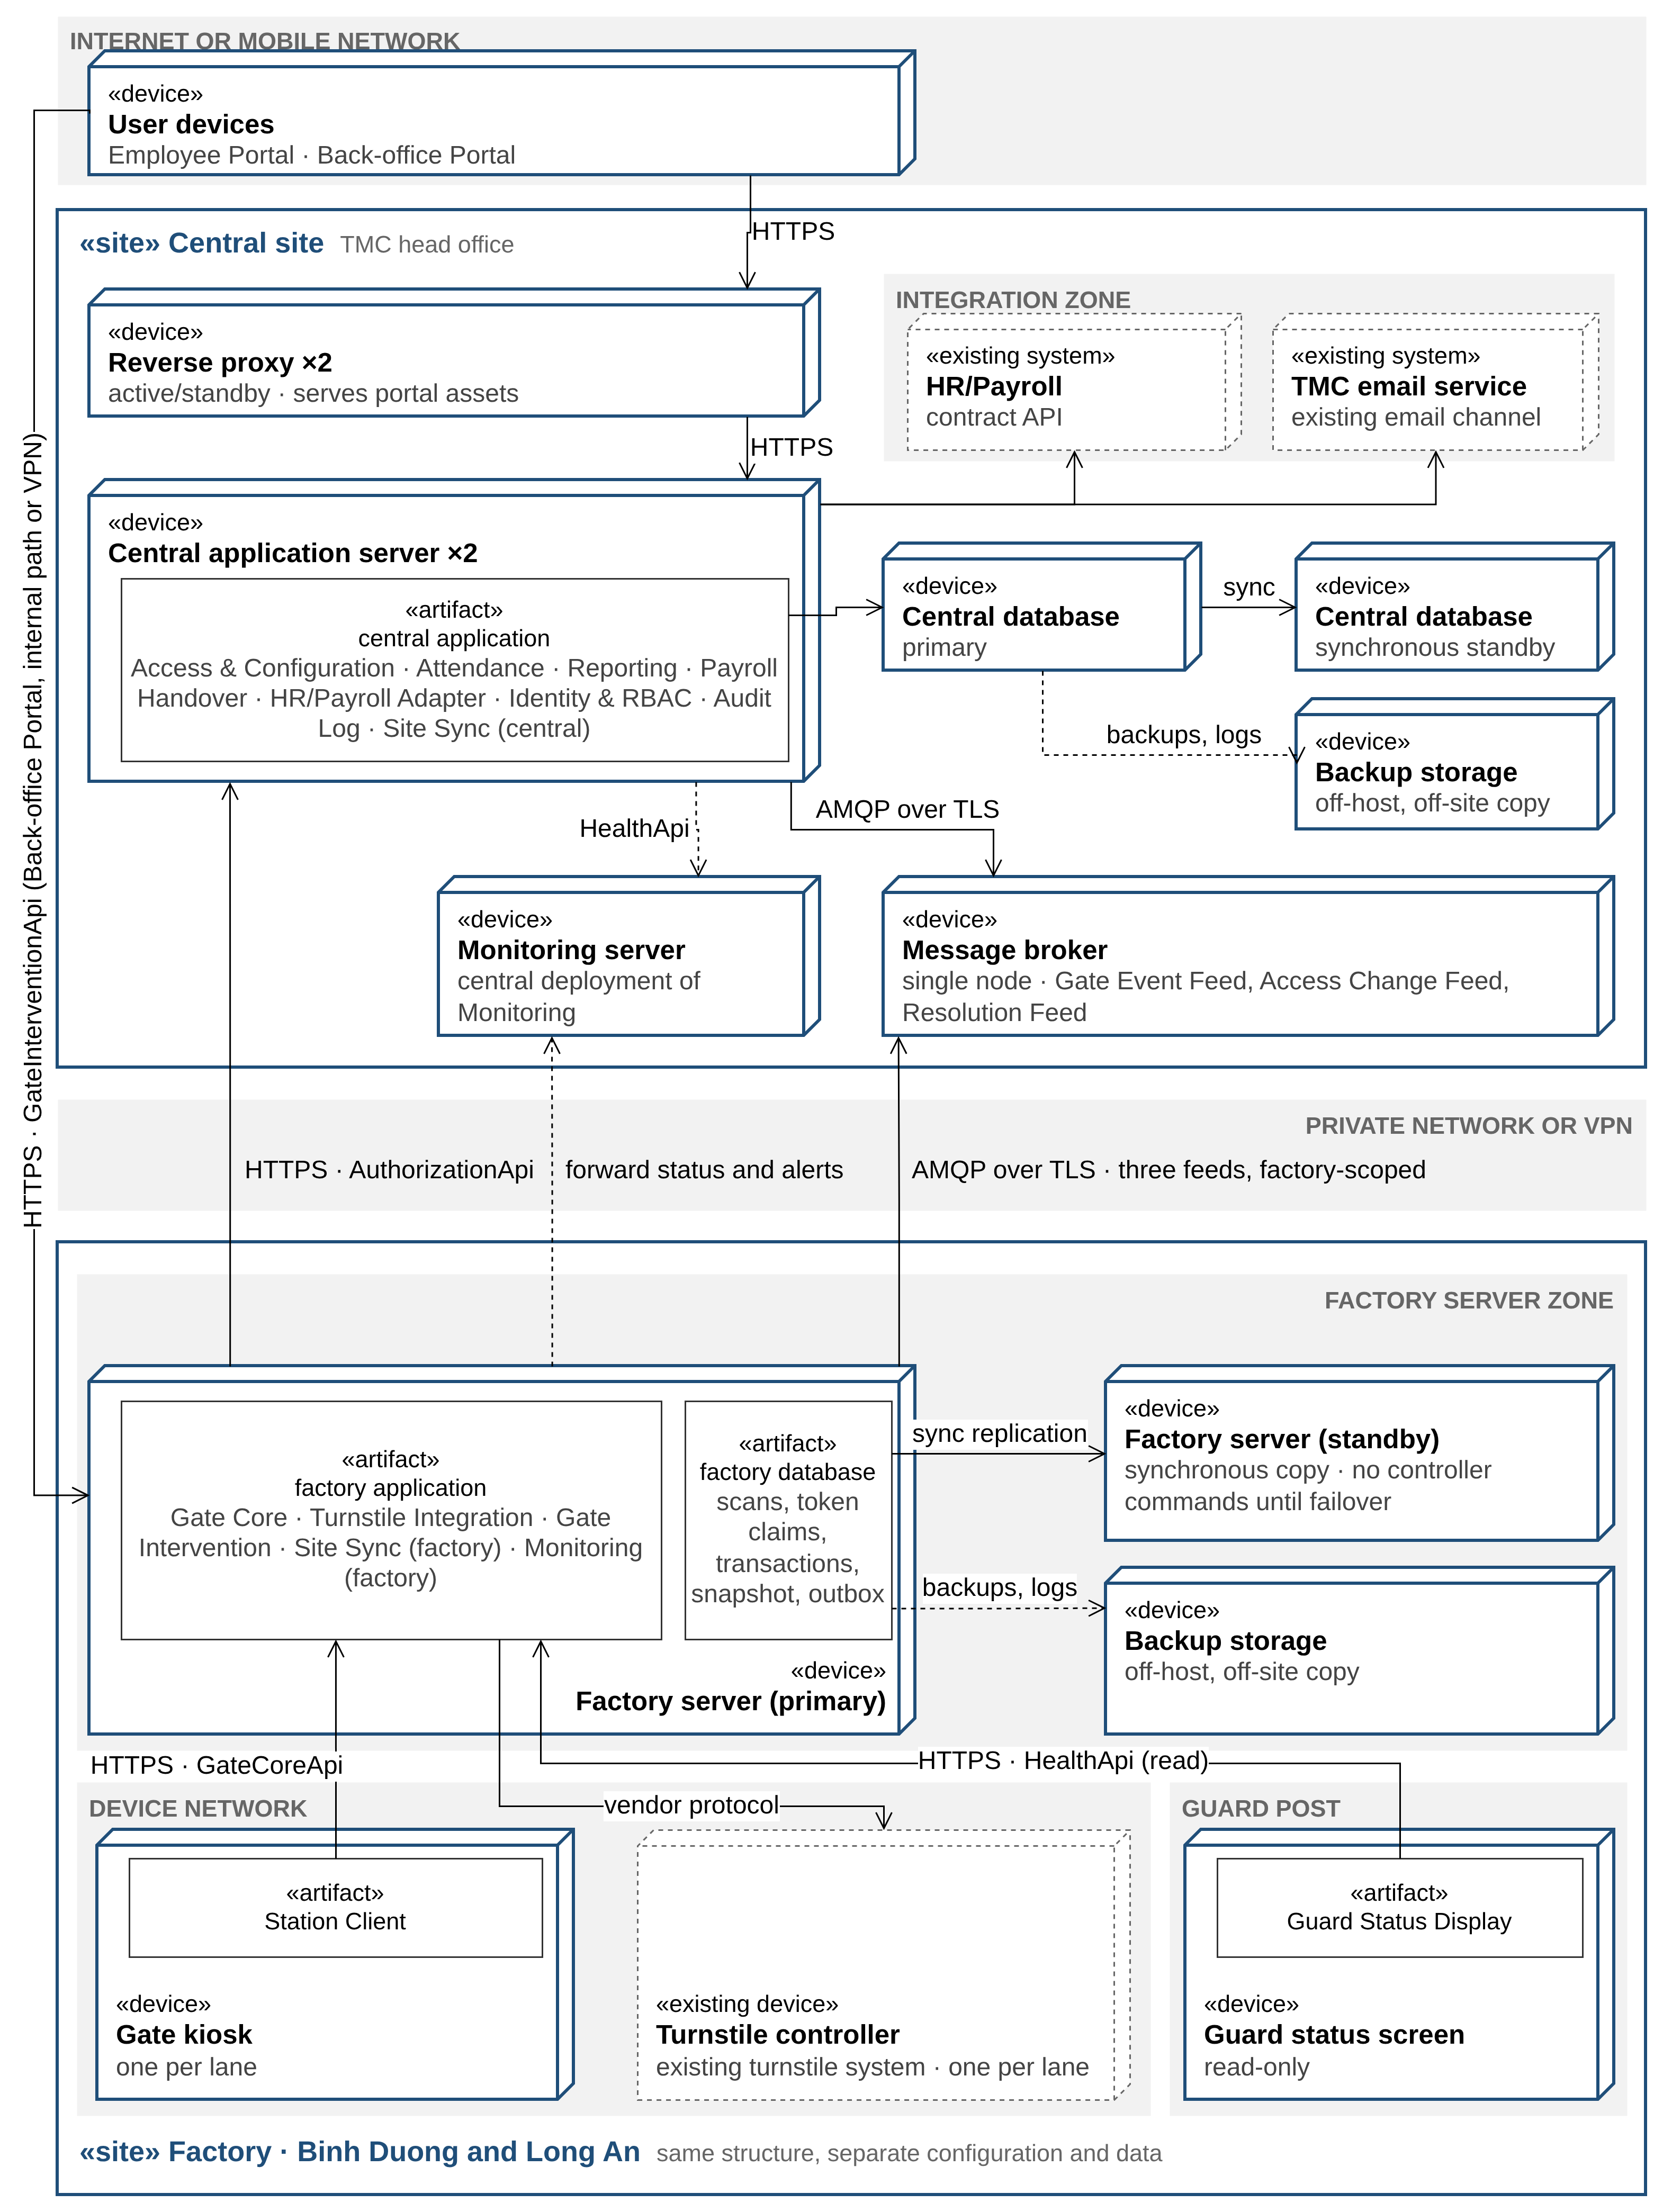
\includegraphics[width=450.0pt,height=560.0pt,keepaspectratio]{diagram/deployment/figure-5-1-deployment.png}}{\fbox{\parbox{300pt}{\centering\vspace{20pt}Figure being redrawn\vspace{20pt}}}}
\par\vspace{6pt}
\textbf{Figure 5.1. Deployment View}
\phantomsection\addcontentsline{lof}{figure}{\protect\numberline{5.1}Deployment View}
\end{minipage}

\medskip

\Needspace{6\baselineskip}
Figure 5.1 is split into three areas:

\begin{itemize}[leftmargin=36pt, itemsep=2pt, topsep=4pt, parsep=2pt]
  \item \textbf{Factory sites} (Binh Duong and Long An) share one structure with separate configuration and data. Kiosks and controllers sit in a device network that is separated from the user network. A primary and a standby factory server run the factory application and database, and the guard status screen reads factory Monitoring over the LAN.
  \item \textbf{Central site} has the reverse proxy pair, two central application instances, the central database pair, the message broker, the monitoring server, and backup storage.
  \item \textbf{External systems and user devices} are the existing turnstile controllers at each factory, HR/Payroll, TMC's email service, and the devices that run Employee Portal and Back-office Portal.
\end{itemize}

We draw the deployment in UML. Nodes labelled \guillemotleft device\guillemotright{} belong to the proposed deployment, and dashed-outline nodes are existing or external systems. Boxes labelled \guillemotleft artifact\guillemotright{} are deployed software or data, and shaded bands mark network or security zones. Solid arrows are communication paths labelled with protocols; dashed arrows are transfers of monitoring data, backups, or logs.

\Needspace{6\baselineskip}
The diagram shows two properties of the deployment:

\begin{itemize}[leftmargin=36pt, itemsep=2pt, topsep=4pt, parsep=2pt]
  \item \textbf{The QR flow stays in the factory.} Links from kiosks to the factory application and from the application to the controllers stay inside the factory network. An ordinary QR scan uses local eligibility data and waits for neither the broker nor a central call. The factory application calls central Identity \& RBAC only for assistance and intervention operations.
  \item \textbf{The factories do not depend on each other.} They never read each other's databases, so a failure at one factory does not directly stop the other. Their shared central dependencies, such as QR issuance, authorization of support operations, and access-right updates, are discussed in Section 5.7.3.
\end{itemize}

\Needspace{9\baselineskip}
\subsection*{5.2. Nodes and Component Mapping}

\phantomsection
\addcontentsline{toc}{subsection}{5.2. Nodes and Component Mapping}


Table 5.1 lists the nodes, how many of each we propose, and what they run. A node can be a physical server, a virtual machine, or another runtime environment.

\begin{longtable}{|>{\raggedright\arraybackslash}p{88pt}|>{\raggedright\arraybackslash}p{82pt}|>{\raggedright\arraybackslash}p{128pt}|>{\raggedright\arraybackslash}p{108pt}|}
\hline
\multicolumn{1}{|>{\columncolor{tableheader}\centering\arraybackslash}p{88pt}|}{\textbf{Node}} & \multicolumn{1}{>{\columncolor{tableheader}\centering\arraybackslash}p{82pt}|}{\textbf{Site and count}} & \multicolumn{1}{>{\columncolor{tableheader}\centering\arraybackslash}p{128pt}|}{\textbf{Runs or stores}} & \multicolumn{1}{>{\columncolor{tableheader}\centering\arraybackslash}p{108pt}|}{\textbf{Notes}} \\
\hline
\endhead
\multicolumn{4}{c}{\rule{0pt}{20pt}\normalsize\textbf{Table 5.1. Proposed Nodes}} \\
\endlastfoot
Gate kiosk & Each factory; one per lane & Station Client & Device network; device identity tied to factory and lane. \\
\hline
Turnstile controller & Each factory; one per lane & Existing turnstile system & Called only by Turnstile Adapter. \\
\hline
Guard status screen & Each factory; one or more at the guard post & Guard Status Display & Read-only, on the factory LAN. \\
\hline
Factory server & Each factory; one primary, one standby & Factory application (Gate Core, Turnstile Integration, Gate Intervention, factory deployments of Site Sync and Monitoring) and the factory database & Synchronous database copy; the standby sends no controller commands until failover is complete. \\
\hline
Reverse proxy & Central; one active, one standby & Entry point for users; serves portal assets & Switchover target in Table 5.5. \\
\hline
Central application server & Central; two active instances & Central application (M4--M8, M10, M11, central Site Sync) & Shared database; durable processing claims for background tasks. \\
\hline
Central database server & Central; one primary, one standby & Central database & Synchronous copy; former primary isolated on failover. \\
\hline
Message broker & Central; one node & Gate Event Feed, Access Change Feed, Resolution Feed & Durable storage; recovery target in Table 5.5. \\
\hline
Monitoring server & Central; one & Central deployment of Monitoring & Receives what the factory deployments forward. \\
\hline
Backup storage & Outside the database servers; off-site copy where possible & Database backups and archived transaction logs & Section 5.6.3. \\*
\hline\noalign{\nobreak}
User device & Anywhere & Employee Portal; Back-office Portal & No internal privileges; authorization stays on the server. \\
\hline
\end{longtable}
\phantomsection\addcontentsline{lot}{table}{\protect\numberline{5.1}Proposed Nodes}


\Needspace{6\baselineskip}
Table 5.1 lists what each node runs. The rules below explain how the nodes behave and why:

\begin{itemize}[leftmargin=36pt, itemsep=2pt, topsep=4pt, parsep=2pt]
  \item \textbf{The kiosk only scans and displays.} Station Client does not access the database, decide access rights, or call the controller; only Turnstile Adapter calls the controller API.
  \item \textbf{One active factory server.} The standby may not coordinate opening commands until a controlled failover has finished, and the former primary is isolated first, so that only one deployment writes data and drives the controller. Losing the link to the central site does not by itself trigger failover.
  \item \textbf{Guards see alerts locally.} Factory Monitoring serves the factory's status and alerts to Guard Status Display over the LAN, so guards still see alerts when the WAN link is down. Central Monitoring tracks applications, databases, devices, synchronization lag, and handover progress, and receives what each factory forwards.
  \item \textbf{Support operations need the central site.} Gate Intervention runs at the factory, but its assistance and emergency operations still need authorization from central Identity \& RBAC. A working factory application therefore does not mean that every support function works during a connectivity interruption.
  \item \textbf{Central instances share no memory state.} Neither central instance keeps critical business state only in memory, and background tasks use an exclusive processing claim, so that only one instance runs each task.
  \item \textbf{Modules keep their own data.} Modules may share a database engine, but Reporting and Payroll Handover read through the owning modules' interfaces, not from Attendance or Audit tables. Database failover must stop the former primary from accepting writes after the standby is promoted.
  \item \textbf{The broker is a single node.} It has durable storage and separate publish and consume permissions by source, factory, and message type, and recovers by restart and storage recovery. Source outboxes keep data while it is down, but they do not replace broker redundancy if TMC needs shorter interruptions.
  \item \textbf{Backups live elsewhere.} Backups are kept outside the database servers, so that one server or storage failure cannot destroy both copies.
\end{itemize}

\Needspace{13\baselineskip}
Table 5.2 shows where each component from Chapter 4 runs. Components in the same application call each other through internal interfaces, so a component does not need its own deployed service.

\begin{longtable}{|>{\raggedright\arraybackslash}p{78.5pt}|>{\raggedright\arraybackslash}p{145.5pt}|>{\raggedright\arraybackslash}p{187.5pt}|}
\hline
\multicolumn{1}{|>{\columncolor{tableheader}\centering\arraybackslash}p{78.5pt}|}{\textbf{Module}} & \multicolumn{1}{>{\columncolor{tableheader}\centering\arraybackslash}p{145.5pt}|}{\textbf{Component}} & \multicolumn{1}{>{\columncolor{tableheader}\centering\arraybackslash}p{187.5pt}|}{\textbf{Deployment location and notes}} \\
\hline
\endhead
\multicolumn{3}{c}{\rule{0pt}{20pt}\normalsize\textbf{Table 5.2. Component-to-Node Mapping}} \\
\endlastfoot
M1 Gate Core & Gate Transaction Processor; \newline Access Decision; Eligibility \newline Snapshot & Application at each factory. Each \newline deployment processes only its \newline factory's data; durable data resides \newline in the factory database. \\
\hline
M2 Turnstile \newline Integration & Turnstile Adapter & Factory application, connected to \newline the controller system within the \newline local network. \\
\hline
M3 Gate \newline Intervention & Gate Intervention & Factory application. Authorizes \newline operations through Identity \& \newline RBAC at the central site. \\
\hline
M4 Access \& \newline Configuration & Access Rights Management; \newline QR Credential Issuance; \newline Email Link Sender; \newline Gate Station Management; \newline Work Schedule Policy & Central application. Manages \newline authoritative data, sends authenticated QR-display links through TMC's existing email service, and supplies updates to factories. \\
\hline
M5 Attendance & Attendance Consolidation; \newline Attendance Review & Central application; consolidated data and review records reside in the central database. \\
\hline
M6 Reporting & Reporting & Central application; calls data-owning modules in-process and keeps no business-data copy. \\
\hline
M7 Payroll \newline Handover & Payroll Handover & Central application; batch state resides in the central database. Background work uses an exclusive processing claim. \\
\hline
M8 HR/Payroll \newline Integration & HR/Payroll Adapter & Central application, using the \newline authorized integration connection to \newline HR/Payroll. \\
\hline
M9 Site Sync & Site Sync & Deployed at each factory and at the \newline central site. These deployments \newline coordinate through the broker using \newline shared event contracts. \\
\hline
M10 Identity \newline \& Access \newline Control & Identity \& RBAC & Central application; factory support operations reach it over the protected central connection. \\
\hline
M11 Audit & Audit Log & Central application; source evidence arrives asynchronously and the central copy resides in the central database. \\
\hline
M12 \newline Monitoring \& \newline Operations & Monitoring & Central deployment for the whole system. A factory deployment inside each factory application keeps local status and alerts readable over the LAN and forwards its records to the central deployment. \\
\hline
M13 Clients & Station Client & Kiosk at each factory lane. \\
\hline
M13 Clients & Guard Status Display & Fixed screen at each factory guard post, on the factory LAN. Read-only; authenticated by a device identity checked at the factory. \\*
\hline\noalign{\nobreak}
M13 Clients & Employee Portal; \newline Back-office Portal & Interface assets are served from the \newline central site; the interfaces execute \newline on user devices. \\
\hline
\end{longtable}
\phantomsection\addcontentsline{lot}{table}{\protect\numberline{5.2}Component-to-Node Mapping}


Eligibility Snapshot only supports decisions at the factory; Access Rights Management and Gate Station Management at the central site remain the authoritative source. Site Sync and Monitoring have several deployments but one logical responsibility each. The broker only delivers messages: it does not process attendance or approve cases.

\Needspace{6\baselineskip}
\textbf{Packaging and runtime.} We propose the following packaging, to be confirmed with TMC's IT team:

\begin{itemize}[leftmargin=36pt, itemsep=2pt, topsep=4pt, parsep=2pt]
  \item \textbf{Two container images.} The factory application and the central application are each built as one container image. Both factories run the same factory image with their own configuration, so we always know which version each site runs and can return to the previous image if a release fails.
  \item \textbf{Docker on each server.} The images run under Docker on the factory servers and the central application servers. The broker, the databases, and the reverse proxy run as separate services on their own nodes (Table 5.1).
  \item \textbf{No Kubernetes.} The system has only a few nodes per site, so an orchestration platform would add operating cost without a clear benefit. It would also be risky at the factory: only one factory instance may drive the controller, and failover must isolate the former primary first, so an orchestrator must never start a second active copy on its own. If TMC already runs Kubernetes, the images can run there with one active factory instance per site.
  \item \textbf{Rolling upgrades.} Because APIs and events carry versions, the two factories and the central site do not have to be upgraded together. The central instances are upgraded one at a time, and each factory is upgraded outside its shift-change peaks.
  \item \textbf{Clients.} Station Client is installed on each kiosk and Guard Status Display on each guard screen. Employee Portal and Back-office Portal are served as static assets by the reverse proxy and run in the user's browser; authorization and business processing stay on the server. A mobile app, if TMC provides one, uses only the employee-facing contracts.
\end{itemize}

\Needspace{9\baselineskip}
\subsection*{5.3. Communication Paths}

\phantomsection
\addcontentsline{toc}{subsection}{5.3. Communication Paths}


Calls that need an immediate answer are synchronous with bounded waiting times, and data that can be processed later goes through durable messaging channels. We propose HTTPS for APIs and AMQP over TLS for the broker; controller and HR/Payroll links follow the real external APIs, and we do not assume capabilities that have not been confirmed. Table 5.3 lists the connections between nodes and external systems.

\begin{longtable}{|>{\raggedright\arraybackslash}p{95.5pt}|>{\raggedright\arraybackslash}p{147.5pt}|>{\raggedright\arraybackslash}p{168.5pt}|}
\hline
\multicolumn{1}{|>{\columncolor{tableheader}\centering\arraybackslash}p{95.5pt}|}{\textbf{From $\rightarrow$ To}} & \multicolumn{1}{>{\columncolor{tableheader}\centering\arraybackslash}p{147.5pt}|}{\textbf{Contract or purpose}} & \multicolumn{1}{>{\columncolor{tableheader}\centering\arraybackslash}p{168.5pt}|}{\textbf{Proposed communication}} \\
\hline
\endhead
\multicolumn{3}{c}{\rule{0pt}{20pt}} \\
\endfoot
\multicolumn{3}{c}{\rule{0pt}{20pt}\normalsize\textbf{Table 5.3. Connections between Nodes and External Systems}} \\
\endlastfoot
Kiosk $\rightarrow$ Factory application & GateCoreApi: submitScan, getScanStatus & HTTPS within the factory network; kiosk authentication and factory/lane scope restrictions. \\
\hline
Back-office Portal $\rightarrow$ Gate Intervention & GateInterventionApi: recordAssistedAccess, authorizeAssistedOpen, emergencyRelease, resetEmergency & HTTPS over an internal access path or VPN; server-side authorization for each operation. \\
\hline
Gate Intervention $\rightarrow$ Central Identity \& RBAC & AuthorizationApi: identity, action, and scope checks & HTTPS over a protected connection with a timeout; authorization is not bypassed on failure. \\
\hline
Factory application $\rightarrow$ Factory database & Persist states, transactions, snapshots, audit records, and outbox entries & Protected database protocol; least-privilege accounts. \\
\hline
Turnstile Adapter $\rightarrow$ Controller API & Turnstile command ports (openGate, closeGate, emergency release and reset); PASSAGE and LANE\_CLEAR are passed back to Gate Core through IPassageEvents & Vendor-supported protocol; TLS where supported, with connections restricted to the device network. \\
\hline
Factory Site Sync $\leftrightarrow$ Central broker $\leftrightarrow$ Central Site Sync & Gate Event Feed, Access Change Feed, Resolution Feed & AMQP over TLS; publishing and consumption permissions scoped by factory, source, and message type. \\
\hline
Event sources $\rightarrow$ Central Audit Log & AuditApi.append: transfer durably persisted audit evidence & Durable asynchronous channel; source validation and duplicate-safe processing. \\
\hline
User devices $\rightarrow$ Reverse proxy $\rightarrow$ Central application & Employee and management APIs & HTTPS; user authentication and server-side authorization and scope checks. \\
\hline
Central application $\rightarrow$ Central database & Read and write data according to module ownership & Protected database protocol; no direct database exposure to clients. \\
\hline
HR/Payroll Adapter $\rightarrow$ HR/Payroll API & Implementation of IPayrollSubmission & Protocol defined by the HR/Payroll contract; protection of integration credentials and handover data. \\
\hline
Central Access \& Configuration $\rightarrow$ TMC email service & Email Link Sender: deliver an authenticated link to the fresh QR display & Existing company email channel; no static QR image or reusable token in the message. \\
\hline
Data sources $\rightarrow$ Monitoring (factory or central deployment) & HealthApi: report health, errors, latency, and processing progress & Asynchronous transmission over protected connections; business flows do not wait for Monitoring to receive the data. \\
\hline
Guard Status Display $\rightarrow$ Factory Monitoring & HealthApi: read the factory's current status and active alerts & HTTPS within the factory network; device identity checked at the factory; read-only. The screen shows that its data is stale when the connection is lost. \\*
% Keep these two rows together without the break point inserted by longtable's hline.
\noalign{\nobreak}\multispan{3}\unskip\leaders\hrule height\arrayrulewidth\hfill\cr\noalign{\nobreak}
Factory Monitoring $\rightarrow$ Central Monitoring & Forward status, alerts, and measurements & Protected connection over the WAN; records are kept at the factory while the link is down. \\
\hline
\end{longtable}
\phantomsection\addcontentsline{lot}{table}{\protect\numberline{5.3}Connections between Nodes and External Systems}


Calls inside one application, such as Gate Transaction Processor to Access Decision, are internal interface calls, not network connections. Database replication and backup transfers use their own access-restricted connections, encrypted as far as the storage platform allows.

\textbf{Message delivery.} Each owning component stores the business change and its event together. Site Sync delivers persisted events through the broker, and consumers apply them by eventId and version (ADR-05). For reconciliation, Attendance Review tracks the matching ResolutionApplied after Gate Core applies the decision.

\subsection*{5.4. Response Time and Lane Capacity}

\phantomsection
\addcontentsline{toc}{subsection}{5.4. Response Time and Lane Capacity}

NFR-01 measures the time from reading the QR code to showing the opening result at the kiosk. The measured path covers validation, the ACCEPTED write, the openGate call with its OPEN\_CONFIRMED result, and the durable write of the opening result. Passage may happen later, and attendance recording, LANE\_CLEAR, and closeGate are outside the 2-second interval.

\Needspace{24\baselineskip}
Table 5.4 splits the 2 seconds over the factory-local flow. The values are targets for testing. Degraded mode uses the same local path, so the budget applies in both normal and degraded mode while the factory still accepts automatic scans.

\begin{longtable}{|>{\raggedright\arraybackslash}p{383.5pt}|>{\raggedright\arraybackslash}p{41.5pt}|}
\hline
\multicolumn{1}{|>{\columncolor{tableheader}\centering\arraybackslash}p{383.5pt}|}{\textbf{Processing stage}} & \multicolumn{1}{>{\columncolor{tableheader}\centering\arraybackslash}p{41.5pt}|}{\textbf{Budget}} \\
\hline
\endhead
\multicolumn{2}{c}{\rule{0pt}{20pt}\normalsize\textbf{Table 5.4. Proposed Response-Time Budget for a Confirmed Gate Opening}} \\
\endlastfoot
Station Client receives the QR code and prepares the request & 100 ms \\
\hline
Request transmission to the factory application and request handling & 150 ms \\
\hline
QR validation, eligibility-data lookup, and access checks & 150 ms \\
\hline
Durable persistence of the accepted scan, token claim, and traceability data & 250 ms \\
\hline
Controller invocation and receipt of OPEN\_CONFIRMED & 700 ms \\
\hline
Durable persistence of the opening result, audit evidence, and outbox event & 350 ms \\
\hline
Response transmission and display at the kiosk & 100 ms \\
\hline
\textbf{Total allocated budget} & \textbf{1,800} \textbf{ms} \\*
\hline\noalign{\nobreak}
\textbf{Reserve within the two-second limit} & \textbf{200 ms} \\
\hline
\end{longtable}
\phantomsection\addcontentsline{lot}{table}{\protect\numberline{5.4}Proposed Response-Time Budget for a Confirmed Gate Opening}


\Needspace{6\baselineskip}
The budget comes with two rules:

\begin{itemize}[leftmargin=36pt, itemsep=2pt, topsep=4pt, parsep=2pt]
  \item \textbf{Durability is never skipped.} Both durable-write steps include the standby acknowledgement required by synchronous replication. If that setup cannot meet the budget, the deployment is tuned or changed and tested again.
  \item \textbf{Deadlines.} Gate Transaction Processor checks the remaining deadline before it starts an opening command, and an expired request never starts one. If the command may already have been sent, an expired deadline does not prove that the controller did not execute it.
\end{itemize}

Table 5.4 is an allocation of the limit, not a measurement; the design must still be tested against NFR-01 at the shift-change load.

\textbf{Lane capacity.} A 2-second response does not show that the gates can carry the shift-change load, so the site survey also checks lane capacity (AC-03). For each direction, entry and exit, we estimate
\[ \mathrm{lanes} \geq \left\lceil \frac{\mathrm{peak\ rate} \times \mathrm{gate\ cycle\ time}}{\mathrm{target\ utilization}} \right\rceil \]
The peak rate is about 1.33 events per second per factory (400 events in 5 minutes), but it counts entries and exits together, so the survey must split it by direction. The gate cycle time runs from ACCEPTED until the lane is released and must be measured on the real turnstiles; it is not the 15-second passage-observation limit. TMC sets the target utilization to leave room for queues and rescans. We do not fix the number of lanes until these values are measured.

\Needspace{9\baselineskip}
\subsection*{5.5. Security Boundaries}

\phantomsection
\addcontentsline{toc}{subsection}{5.5. Security Boundaries}


The deployment uses the following network and security boundaries:

\begin{itemize}[leftmargin=36pt, itemsep=2pt, topsep=4pt, parsep=2pt]
  \item \textbf{Factory zones.} The factory network is split into kiosk, application, and controller-device zones, and firewalls allow only the connections that are needed between them.
  \item \textbf{Kiosk identity.} Each kiosk has a device identity tied to its factory and lane, for example a device certificate. The server checks each request against the registered configuration instead of trusting the factory or lane values in the request. A kiosk may only submit scans and query their status; it cannot call recordIntervention, change configuration or access rights, or trigger emergency opening.
  \item \textbf{Controller access.} Only Turnstile Adapter connects to the controllers; users, kiosks, and the central application have no path that bypasses the factory application. If a controller does not support TLS, we record this limitation and rely on isolation in the device network and restricted sources; we do not call that link end-to-end TLS.
  \item \textbf{Central entry point.} The reverse proxy is the entry point for user access. The central application, database, and broker are not exposed to external networks, and factories reach only the endpoints and channels they need.
  \item \textbf{Factory scope.} Site Sync at a factory may publish events and receive updates only within that factory's scope. Factories cannot publish authoritative access-right changes or approval decisions on behalf of Attendance Review.
  \item \textbf{Integration credentials.} HR/Payroll Adapter uses a dedicated integration account limited to the handover contract. Kiosks and factory applications never access the payroll database or use the adapter's credentials.
  \item \textbf{Verification keys.} Factories receive only the material they need to verify QR codes, and holding it does not let a factory issue tokens. Key management and replay prevention are described in Chapter 7.
  \item \textbf{User access and personal data.} The reverse proxy and application services check operation and data-scope permissions before any request reaches central data. Database, broker, and backup access is limited to the matching service and administrator accounts. Chapter 7 covers audit access and personal-data protection for these records.
\end{itemize}

\Needspace{9\baselineskip}
\subsection*{5.6. Data Persistence and Availability}

\phantomsection
\addcontentsline{toc}{subsection}{5.6. Data Persistence and Availability}

\subsubsection*{5.6.1. Persistence}

\phantomsection
\addcontentsline{toc}{subsubsection}{5.6.1. Persistence}


Each site keeps its own records durably:

\begin{itemize}[leftmargin=36pt, itemsep=2pt, topsep=4pt, parsep=2pt]
  \item \textbf{Factory database.} It holds scan and gate-cycle states, token claims, passage evidence, source attendance transactions, audit evidence, support cases, the eligibility data used for decisions, duplicate-prevention data, and pending events. Gate Transaction Processor stores ACCEPTED and the token claim together before a controller command, and a confirmed passage is stored with its attendance transaction and outgoing event. Controller actions are outside the database transaction, so recovery may need controller evidence or reconciliation.
  \item \textbf{Central database.} It holds authoritative access rights and configuration, shift schedules, consolidated attendance, review cases, decisions and evidence, audit copies, HR/Payroll batch content and receipt history, and accounts and permissions. Attendance Review tracks application at Attendance Consolidation and Gate Core separately. Payroll Handover stores batch identity and content before external submission, and competing central instances use durable processing claims.
\end{itemize}

\subsubsection*{5.6.2. Redundancy and Failover}

\phantomsection
\addcontentsline{toc}{subsubsection}{5.6.2. Redundancy and Failover}

The primary database acknowledges a commit only after the data is stored as the synchronous replication setting requires. Acknowledged commits therefore survive a primary failure while the standby is intact. The price is that the standby becomes part of every write: if the commit conditions cannot be met, the system does not silently switch to weaker persistence while still reporting success.


At a factory, this rule has a direct consequence. If the primary database cannot get the required standby acknowledgement, for example because the standby or the replication link has failed, the factory stops accepting new scans that would lead to an opening command. Cycles that are already open must still end safely. Gate Core continues automatic closing only while it can still durably record LANE\_CLEAR and the single reserved close command; otherwise guards close or secure the lane under the approved safety procedure. Passage or attendance that could not be stored is reconciled from controller evidence after recovery, and in-progress scans are resolved the same way. Guards use the manual procedure for new arrivals, and attendance recording is never moved to the kiosk to get around the database failure. The remedy is to repair the standby or the replication link, not to fail over, because the primary is still working. We keep this policy because ADR-10 does not allow durability to be weakened during a failure.


Failover covers the other case: the primary fails and an eligible standby can take over. After promotion, the new primary has no synchronous partner, so under the same rule it still cannot accept new scans until a replica can acknowledge commits again. Changing roles is therefore not the end of recovery. The 5-minute target in Table 5.5 is measured until the commit conditions are restored and new scans are accepted. Meeting it may need a second standby or a replica that can be rebuilt quickly; testing decides which.


At the central site, the reverse proxy stops routing requests to an unavailable application instance, and the other instance carries on from database state. Database failover must isolate the former primary before the promoted database accepts writes.


Replication does not protect against every failure. Accidental deletion, wrong updates, or corrupted data are copied to the standby as well, and losing both copies or a whole site still needs a backup restore.

\subsubsection*{5.6.3. Backup and Restore}

\phantomsection
\addcontentsline{toc}{subsubsection}{5.6.3. Backup and Restore}

We propose a daily full database backup and continuous transaction-log archiving, with log transfer normally no more than five minutes behind. Backups are stored outside the database servers, with an off-site copy where the infrastructure allows. They cover scan states, token claims, transactions, decisions, audit records, batches, outboxes, and deduplication markers. Configuration, active contracts, and the information needed for key recovery need their own retention.


After a restore, the application does not accept new scans until database state, application versions, unfinished scans, eligibility data, and replay-prevention state have been checked. A restore may take the data back to an earlier point in time, so tokens used and commands executed after that point must be handled under a safe recovery policy. They are never treated as if they had not been processed.


\Needspace{6\baselineskip}
Data-loss and recovery objectives depend on the failure scope:


\begin{itemize}[leftmargin=36pt, itemsep=2pt, topsep=4pt, parsep=2pt]

  \item For an isolated primary-database failure with an intact synchronous standby, the objective is to lose no acknowledged commits.

  \item For failures that need a backup restore, the initial objective is a data-loss window of no more than five minutes, provided log archiving works correctly.

  \item Site-wide loss, simultaneous failures, and incomplete log transfer are assessed separately.

\end{itemize}

The five-minute window applies only to failures; it does not relax NFR-02's requirement to keep attendance records during normal operation. Any part that cannot be recovered exactly is recorded and reconciled.

\subsection*{5.7. Failure Handling and Recovery}

\phantomsection
\addcontentsline{toc}{subsection}{5.7. Failure Handling and Recovery}

Failures are handled with explicit thresholds, a bounded degraded mode at the factories, and a fixed recovery order after reconnection.

\Needspace{9\baselineskip}
\subsubsection*{5.7.1. Operating Thresholds}

\phantomsection
\addcontentsline{toc}{subsubsection}{5.7.1. Operating Thresholds}


Table 5.5 sets initial thresholds for configuration and testing. TMC must approve the two access-right limits (60 seconds and 30 minutes) because they decide how quickly a revocation takes effect.

\begin{longtable}{|>{\raggedright\arraybackslash}p{95.5pt}|>{\raggedright\arraybackslash}p{156.5pt}|>{\raggedright\arraybackslash}p{158.5pt}|}
\hline
\multicolumn{1}{|>{\columncolor{tableheader}\centering\arraybackslash}p{95.5pt}|}{\textbf{Item}} & \multicolumn{1}{>{\columncolor{tableheader}\centering\arraybackslash}p{156.5pt}|}{\textbf{Threshold or objective}} & \multicolumn{1}{>{\columncolor{tableheader}\centering\arraybackslash}p{158.5pt}|}{\textbf{Application}} \\
\hline
\endhead
\multicolumn{3}{c}{\rule{0pt}{20pt}\normalsize\phantomsection\addcontentsline{lot}{table}{\protect\numberline{5.5}Proposed Operating Thresholds and Recovery Objectives}\textbf{Table 5.5. Proposed Operating Thresholds and Recovery Objectives}} \\
\endlastfoot
Kiosk response while automatic scans are accepted & No more than 2 seconds, in normal and degraded mode & The NFR-01 limit, not a configurable threshold for relaxing the requirement. \\
\hline
Controller interaction during a QR scan & Initial budget of 700 ms, without exceeding the scan's remaining deadline & Applies only to openGate in the QR flow. If the deadline has already passed, no command is sent. Expiration after the command may have been sent is treated as an undetermined outcome. \\
\hline
Controller interaction during an assisted opening & Initial time limit of 3 seconds, configurable & A threshold we chose for the guard-assisted flow, separate from the kiosk response target in NFR-01. A timeout after the command may have been sent is undetermined, and the command is never resent. \\
\hline
QR token validity (I-09) & 60 seconds from issuance & Reject the expired token for its scan; other valid tokens may still be accepted. \\
\hline
Passage observation (I-05) & Initial 15 seconds after OPEN\_CONFIRMED & Gate Core flags missing passage for review. This timer never authorizes closeGate. \\
\hline
Component health checks & Every 5 seconds; alert after 3 consecutive failures & Approximately 15-second detection target, to be measured in testing. Failures encountered by actual requests are handled immediately. \\
\hline
Access-right update progress confirmation & Proposed interval of 10 seconds & Confirmation must identify versions and applied progress, not merely indicate that the connection is alive. \\
\hline
Normal age of access-right data (I-10) & No more than 60 seconds from the source's confirmation of a valid data watermark, allowing for transmission delay and clock skew & Normal automatic acceptance. Past this limit the factory switches to degraded mode if the other conditions in Section 5.7.2 still hold. \\
\hline
Degraded-mode limit (I-10) & Less than 30 minutes from the same watermark & Accept only signed, unexpired, unclaimed QR codes and flag each transaction. Once the data is 30 minutes old, or continuity is lost, stop automatic acceptance at all lanes; new scans return CANNOT PROCESS. \\
\hline
Clock error used for validity checks & Below 2 seconds against the time used for QR issuance and checkpoints & Continue only while the factory has a measured error bound below the limit. Stop QR processing when the bound is lost or reaches or exceeds the limit (Section 5.7.2). \\
\hline
Outbox storage capacity & Sized for at least 48 hours under the load model; warning at 70\% utilization and critical alert at 85\% & Do not delete events that have not met delivery conditions merely to free storage. \\
\hline
Failover after a primary failure & No more than 5 minutes from the start of the procedure until commit conditions are restored and new scans are accepted & Only when the primary has failed and an eligible standby can take over; the former primary is isolated first. A failed standby is repaired, not used for failover (Section 5.6.2). \\
\hline
Recovery of the broker and Access Change Feed & Proposed: no more than 10 minutes, to be verified. Measured from detecting the broker outage until each factory has applied the backlog and advanced its watermark with a new confirmed checkpoint & Leaves a margin before the 30-minute limit in I-10. A longer outage stops automatic scans at the factories one after another (Section 5.7.3). \\
\hline
Switchover of the reverse proxy & Proposed: no more than 30 seconds, to be verified. Measured from detecting the proxy failure until a new QR code is issued successfully through the standby proxy & Shortens the interruption to new QR issuance. Codes already shown keep their own 60-second validity and may still expire during the switchover. \\
\hline
Database restoration from backup & Initial target of no more than 30 minutes with the test dataset & Measure until data and service-readiness conditions have been checked; this is not a guarantee for every data volume or failure. \\
\hline
Synchronization after connectivity is restored & Sustained processing rate of at least twice the event-generation rate in the test & Receive new data while reducing the backlog; verify using a representative load model. \\*
\hline\noalign{\nobreak}
HR/Payroll handover & First submission planned at 06:00; internal alert at 10:00; required data available before 12:00 noon on day one & Check overnight shifts and source progress; 06:00 is not a final cutoff. Alerts do not replace confirmation. \\
\hline
\end{longtable}


Outbox capacity is sized from real event counts and sizes, audit data, retransmissions, and a reserve; the load of 800 events in 30 minutes does not last all day. When storage reaches the critical threshold, operators estimate how long data can still be kept. The application stops accepting new scans before space runs short for mandatory transactions and the recovery reserve, not when the database is already full.

\subsubsection*{5.7.2. Eligibility Freshness and Degraded Mode}

\phantomsection
\addcontentsline{toc}{subsubsection}{5.7.2. Eligibility Freshness and Degraded Mode}

Eligibility Snapshot is used only when its data is complete, comes from an authorized source, and meets the version, continuity, and time requirements.


The Access Change Feed keeps sending progress confirmations even when nothing changes, so that a factory can tell how far it has received. Each confirmation carries the time at which the source checked and confirmed the data watermark. The factory advances its watermark only after applying all required data up to that point. Freshness is measured from the source's time, allowing for transmission delay and clock error, so a delayed message does not restart the 60-second limit. Duplicates, older versions, health signals without progress information, and the update time of a single record cannot refresh the watermark.


\Needspace{6\baselineskip}
The QR flow continues only when all of the following conditions hold:


\begin{itemize}[leftmargin=36pt, itemsep=2pt, topsep=4pt, parsep=2pt]

  \item The QR token is valid and unexpired.

  \item Employee data, access rights, lane configuration, and verification keys have the required versions.

  \item No missing sequence or unapplied mandatory update has been detected.

  \item The watermark is within the normal limit, or within the degraded limit described below.

  \item The clock-error bound is known and below 2 seconds.

  \item The factory application, database, and controller are working.

  \item Token claiming and replay prevention work as described in Chapter 7.

  \item Enough storage capacity remains.

\end{itemize}

Losing the connection does not invalidate a token or the snapshot at once, but their limits in Table 5.5 keep running, and an expired token is rejected for its own scan. When the watermark passes 60 seconds, Gate Core switches the factory to degraded mode instead of stopping. Because the watermark may already be a few seconds old when the link fails, this can happen in less than one minute.


\Needspace{6\baselineskip}
\textbf{Degraded mode.} Gate Core keeps the normal flow with three changes:

\begin{itemize}[leftmargin=36pt, itemsep=2pt, topsep=4pt, parsep=2pt]

  \item It accepts only QR codes whose signature is valid under the locally stored key, that are unexpired, bound to this factory, and not yet claimed. Replay protection does not change, because all lanes share the factory's token-claim data.

  \item It marks every ACCEPTED scan, and the attendance transaction created after passage, with a DEGRADED flag and the snapshot version it used.

  \item It writes the start and end of the mode to the audit log and raises an alert through the factory deployment of Monitoring. Guard Status Display shows the alert at the guard post over the factory LAN, and the central deployment receives it when the link returns. The kiosk shows the employee the normal result.

\end{itemize}

The mode ends in one of two ways. If confirmed updates arrive again, Site Sync applies the missing changes and Gate Core returns to normal mode. Attendance Review then compares each DEGRADED transaction with the changes that were applied. A transaction whose employee was suspended, lost access, or was moved to another factory during the window becomes a review case for HR or Security; the others stay flagged in reports. If 30 minutes pass since the last confirmed update, Gate Core returns CANNOT PROCESS for new scans at every lane and guards use the approved manual procedure. In both cases an opened lane still needs passage tracking and safe closing.


We chose 30 minutes because it covers one full shift-change peak (about 800 scans per factory). Every scan in the window is flagged, but only transactions whose employee's access changed during the window become review cases, so HR does not have to check all of them. The value is a configuration parameter, and TMC must approve it together with the revocation risk below.


\textbf{Factory WAN outage and central outage.} New QR codes still come from the central site, but an employee's phone reaches it over the Internet or the mobile network, not over the factory WAN link. During a factory WAN outage, employees can therefore still get fresh codes and pass in degraded mode. A central-site outage is different: QR issuing stops, existing codes expire within 60 seconds, and the automatic flow stops at both factories at about the same time, whatever the state of the snapshot.


Guards switch to the approved manual procedure only when automatic acceptance is no longer allowed. During a central-site outage this happens once existing codes expire. During a factory WAN outage it happens when the watermark reaches the I-10 limit, or earlier if the factory no longer meets another required operating condition, such as a known clock-error bound, durable writes, or snapshot continuity. Each manual entry is recorded as an assisted case that HR must approve (I-04). During a central-site outage, software authorization for assisted opening is also unavailable (Section 5.7.4), so guards keep the record by hand and enter it after recovery. Arrivals average about 27 per minute per factory over the 30-minute shift change, and we assume a peak of about 80 per minute (400 events in 5 minutes). TMC needs a staffing plan for that peak. The software never lets a kiosk open the gate on its own.


Each token is valid at only one factory, and all lanes in that factory share Gate Core's token-claim data. Acceptance during a disconnection is allowed only while replay prevention works and all eligibility-data conditions hold. If token-claim consistency cannot be guaranteed after failover or restoration, the factory stops accepting new scans until safe conditions are re-established.


\textbf{Time during a WAN outage.} The factory application server is the time source for the kiosks and synchronizes with the time used for QR issuance and checkpoints at the central site. What matters is the error against that central time; factory clocks that agree with each other can still all be wrong. Gate Core keeps an error bound: the error measured at the last successful synchronization plus the drift allowed since then, using a drift rate measured for the server in testing. The bound grows while the WAN is down. Gate Core continues QR checks only while the bound is known and below 2 seconds, and stops automatic acceptance when it cannot establish the bound or the bound reaches or exceeds the limit (Table 5.5). The central issuing service follows the same rule for its own clock.


\textbf{Effectiveness of access-right revocation.} Once a factory receives and applies a change, new scans use the updated version. During isolation, the factory may not know that a right has just been revoked at the central site. Automatic acceptance using the old rights is allowed only while the last confirmed watermark is less than 30 minutes old. The revocation itself may arrive later, after reconnection; 30 minutes is not a delivery guarantee. The DEGRADED flag makes every scan in that window easy to find and check later, but it cannot undo an entry that has already happened. If TMC needs immediate revocation, the scans that need that guarantee must check online or stop when the connection is down. The system cannot rely on a disconnected copy and also know every central change at once.

\subsubsection*{5.7.3. Loss of Central Connectivity or Broker Availability}

\phantomsection
\addcontentsline{toc}{subsubsection}{5.7.3. Loss of Central Connectivity or Broker Availability}

When the central site or the broker cannot be reached, the factory keeps new passage-based attendance transactions and other events in its local outbox, and accepts new scans only under the conditions in Section 5.7.2. Passage tracking and closeGate stay local and do not wait for the broker. Operations that need central authorization, such as software-based assistance and emergency opening, may stop. Whether employees can still get new QR codes depends on whether their phones can reach the central application, not on Site Sync.


If only the broker is unavailable, central APIs may continue operating while the central application and database remain available. Gate-transaction delivery, access-right updates, and reconciliation decisions are delayed, and reports may lack recent factory data. Because the Access Change Feed also stops, neither factory receives new checkpoints. Each factory moves to degraded mode when its watermark passes 60 seconds and stops automatic acceptance when it reaches 30 minutes. The factories cross these limits one after another, since their last checkpoints differ. For this reason the recovery target in Table 5.5 covers the whole path, not only restarting the broker.


\textbf{Shared central entry points.} The broker and the reverse proxy are both shared by the two factories, but losing them has different effects. Losing the reverse proxy blocks the route to QR issuance, so automatic scans fail at both factories within about 60 seconds as existing codes expire. Losing the broker only ages the watermark, which leaves up to 30 minutes. We therefore run the reverse proxy as an active/standby pair and keep the broker as a single node with the recovery target in Table 5.5. Two central application instances do not cover either failure.


\textbf{After reconnection.} Site Sync checks versions, applied watermarks, and pending data. Missing access-right updates are fetched as a change sequence or as a complete snapshot from an authorized source, and Access Decision uses them only after the required conditions are checked again, not just because the link is back. Transaction and audit events are resent with their original identifiers. The central site processes backlog and new data together, with resource limits so that catching up does not slow the QR flow. Reports show reception progress and missing data; the timestamp of the newest event does not prove that all earlier events have arrived.

\noindent\begin{minipage}{\linewidth}
\setlength{\parskip}{0pt}
\setstretch{1}
Figure 5.2 shows the recovery order after the link to the central site returns.
\par\vspace{8pt}
\centering
\IfFileExists{diagram/deployment/figure-5-2-reconnect.png}{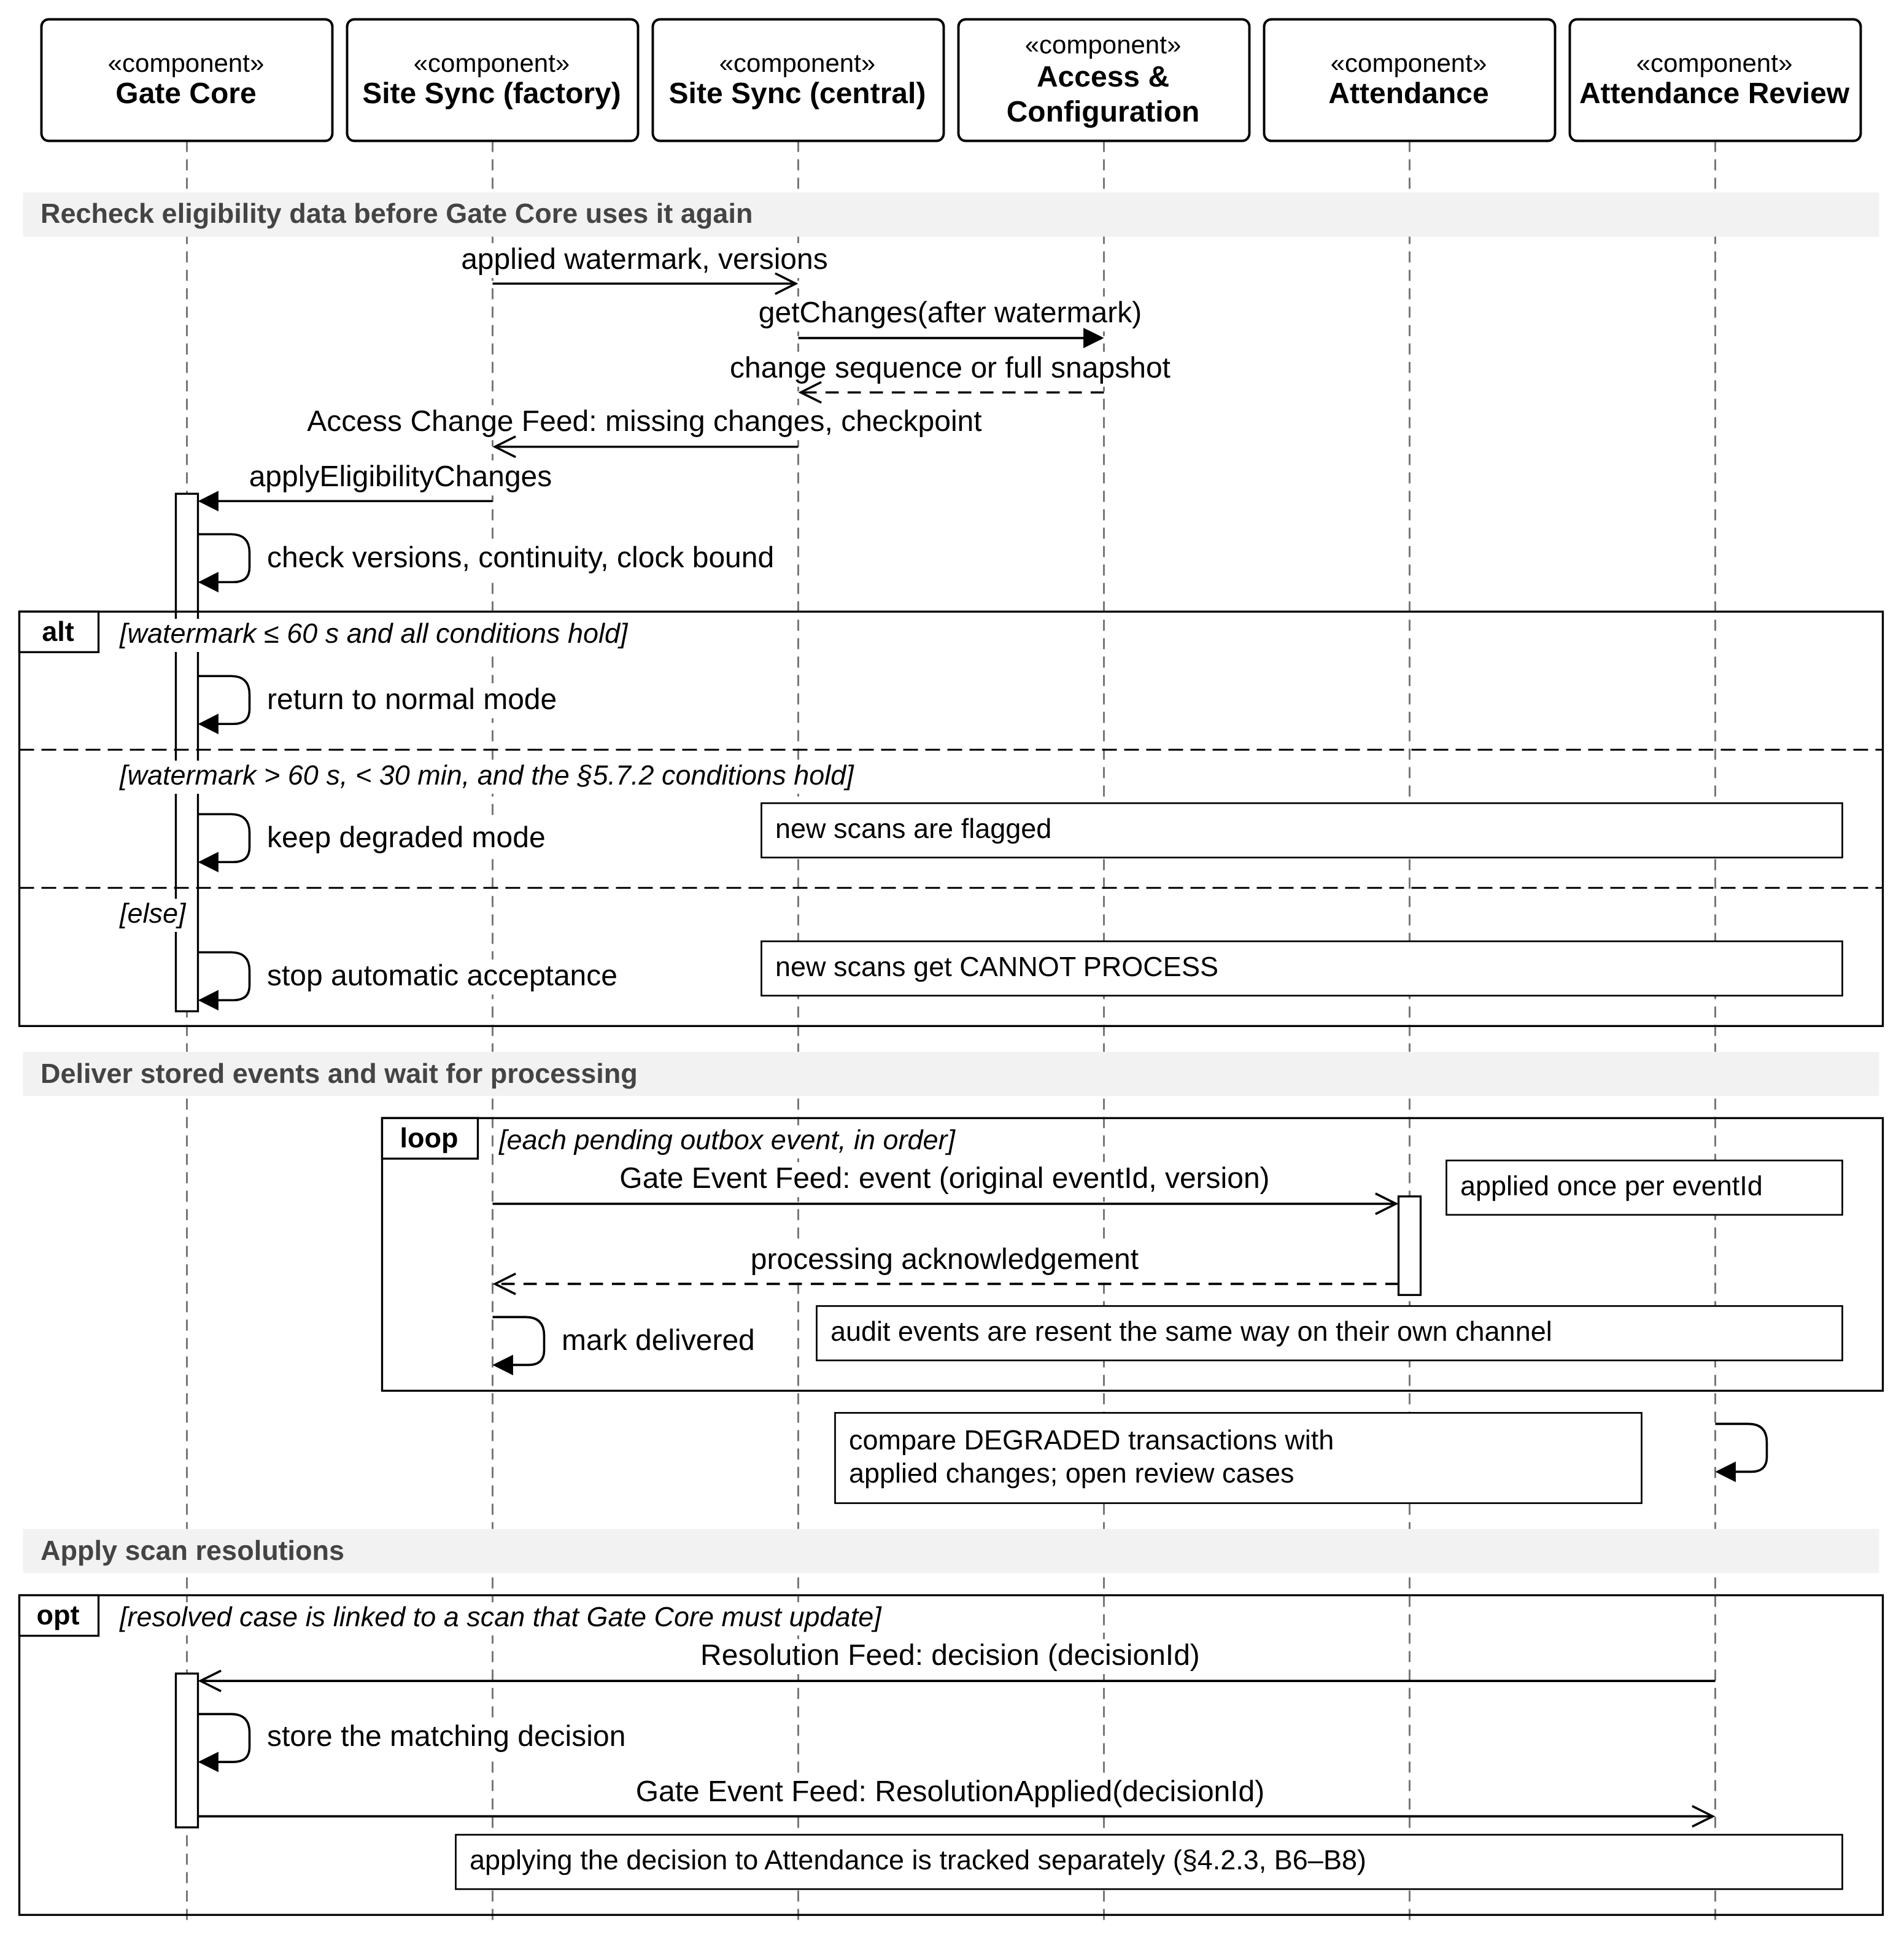
\includegraphics[width=450.0pt]{diagram/deployment/figure-5-2-reconnect.png}}{\fbox{\parbox{300pt}{\centering\vspace{20pt}Figure being redrawn\vspace{20pt}}}}
\par\vspace{4pt}
\textbf{Figure 5.2. Recovery Order after Reconnection}\par
\phantomsection\addcontentsline{lof}{figure}{\protect\numberline{5.2}Recovery Order after Reconnection}
\vspace{6pt}
{\raggedright
In this order, Site Sync rechecks source versions and applied watermarks before Gate Core uses eligibility data again, then sends stored events with their original identifiers and waits for each consumer's processing acknowledgement. When a resolved case is linked to a scan that Gate Core must update, it follows steps B6--B8 of Flow B and is complete only after Gate Core stores the matching decision and returns ResolutionApplied. Applying the decision to Attendance is tracked separately. The Access Change Feed, Gate Event Feed, and Resolution Feed shown here pass through the message broker. No recovery step resends openGate.
\par}
\end{minipage}

\medskip

\Needspace{12\baselineskip}
\subsubsection*{5.7.4. Other Failures}

\phantomsection
\addcontentsline{toc}{subsubsection}{5.7.4. Other Failures}


Three other failure areas need their own handling:

\begin{itemize}[leftmargin=36pt, itemsep=2pt, topsep=4pt, parsep=2pt]
  \item \textbf{Factory application, database, and controller.} A kiosk that loses its response keeps the scanId and queries the stored result after reconnection. During factory-application failover, new scans stop while Gate Transaction Processor examines unfinished states; a persisted ACCEPTED state may already have led to a controller command, so an uncertain opening is queried or reconciled under I-03. A database write failure before ACCEPTED prevents a new opening command. A failure after opening or passage needs recovery from retained controller evidence, and an opened lane still needs safe closing or guard intervention. Controller non-execution, missing passage or LANE\_CLEAR, and uncertain close results follow Table 4.22. Where the controller architecture allows, the fault is limited to the affected lane.
  \item \textbf{Assisted access and emergency.} Gate Intervention needs central Identity \& RBAC authorization for software-based assistance and emergency actions. If that check is unavailable, ordinary software opening stops and guards follow TMC's approved manual or physical safety procedure. The case record, HR approval, emergency reset, and safe closing follow Flow B in Chapter 4. A manual record keeps the actual event time separate from the later entry time.
  \item \textbf{Central processing and HR/Payroll.} After the central site recovers, Site Sync resumes delivery from the source outboxes with the original event identifiers and versions. Attendance Review resumes incomplete decisions with the same decision identifier and waits for the matching application result where one is required. Payroll Handover checks persisted batch states and HR/Payroll receipt evidence; an uncertain batch is queried or resent only under the safe conditions of Flow C. The monthly period is complete only when HR/Payroll has confirmed receipt of all mandatory data, and whether that happened before the deadline is tracked separately.
\end{itemize}

\subsection*{5.8. Responses to the Issues Encountered}

\phantomsection
\addcontentsline{toc}{subsection}{5.8. Responses to the Issues Encountered}

The M2 assignment adds two issues: the system can lose connectivity while an attendance transaction is being processed, and a static QR code can be exposed and misused. For each issue we first look at where the problem can happen, then compare the options we considered, describe the enhancement we chose, and check how far it mitigates the issue and what risk is left. Section 5.8.3 shows where the enhancements sit in the logical and physical architecture. Most of the mechanisms were already built into the design in Chapters 4 to 7, so this section collects them in one place and points to the sections with the details.

\Needspace{9\baselineskip}
\subsubsection*{5.8.1. Connectivity Loss during an Attendance Transaction}

\phantomsection
\addcontentsline{toc}{subsubsection}{5.8.1. Connectivity Loss during an Attendance Transaction}

\textbf{Problem.} One gate transaction crosses several links: the kiosk talks to the factory server, the factory server talks to the turnstile controller, and the factory sends events to the central site over the WAN and the message broker. Any of these links can break after the employee has scanned but before the transaction is finished. If that happens, an attendance record can be lost or stored twice, the gate can open without any evidence, and a factory that has lost contact with the central site can keep using access rights that are no longer current. Table 5.6 lists the points where the connection can fail and what is at stake at each one.

\begin{longtable}{|>{\raggedright\arraybackslash}p{62pt}|>{\raggedright\arraybackslash}p{150pt}|>{\raggedright\arraybackslash}p{199pt}|}
\hline
\multicolumn{1}{|>{\columncolor{tableheader}\centering\arraybackslash}p{62pt}|}{\textbf{Point}} & \multicolumn{1}{>{\columncolor{tableheader}\centering\arraybackslash}p{150pt}|}{\textbf{What can go wrong}} & \multicolumn{1}{>{\columncolor{tableheader}\centering\arraybackslash}p{199pt}|}{\textbf{How the design handles it}} \\
\hline
\endhead
\multicolumn{3}{c}{\rule{0pt}{20pt}\normalsize\phantomsection\addcontentsline{lot}{table}{\protect\numberline{5.6}Where a Gate Transaction Can Break}\textbf{Table 5.6. Where a Gate Transaction Can Break}} \\
\endlastfoot
F1. Kiosk to factory server (LAN) & Gate Core has stored the result, but the response does not reach the kiosk, and the kiosk may send the scan again. & The kiosk keeps the scanId and asks again with the same scanId. Gate Core returns the stored status without a second command or transaction (Section 7.3.2). \\
\hline
F2. Factory server to controller & The openGate reply is lost, so nobody knows whether the gate opened. & ACCEPTED, the token claim, and the gate cycle are stored before openGate. A lost reply becomes UNDETERMINED. The controller is queried where it supports a status query; if it does not, or the result is still unknown, the scan goes to PENDING\_RECONCILIATION. openGate is never resent (ADR-02, Section 4.2.5). \\
\hline
F3. Factory to central site (WAN or broker) & Committed events cannot be delivered, and access-right updates stop arriving. & Events wait in the factory outbox and are resent later with their original identifiers (ADR-05). Access data ages: degraded mode after 60 seconds, no automatic scans from 30 minutes (ADR-06, Section 5.7.2). \\
\hline
F4. Central site unavailable & QR issuing stops, and software approval for assisted access is not available. & Codes already shown expire within 60 seconds, then guards use the approved manual procedure and enter the cases after recovery (Sections 5.7.2 and 5.7.4). \\*
\hline\noalign{\nobreak}
F5. Factory application or database fails & A transaction is cut in the middle of its steps. & Each step is one database transaction. After failover, new scans wait until unfinished states are checked, and an uncertain opening is queried or reconciled (Sections 5.6.2 and 5.7.4). \\
\hline
\end{longtable}

\textbf{Alternatives considered.} Table 5.7 compares four ways of keeping the gates working when a link fails.

\begin{longtable}{|>{\raggedright\arraybackslash}p{96pt}|>{\raggedright\arraybackslash}p{150pt}|>{\raggedright\arraybackslash}p{165pt}|}
\hline
\multicolumn{1}{|>{\columncolor{tableheader}\centering\arraybackslash}p{96pt}|}{\textbf{Option}} & \multicolumn{1}{>{\columncolor{tableheader}\centering\arraybackslash}p{150pt}|}{\textbf{Strength}} & \multicolumn{1}{>{\columncolor{tableheader}\centering\arraybackslash}p{165pt}|}{\textbf{Weakness}} \\
\hline
\endhead
\multicolumn{3}{c}{\rule{0pt}{20pt}\normalsize\phantomsection\addcontentsline{lot}{table}{\protect\numberline{5.7}Alternatives for Handling Connectivity Loss}\textbf{Table 5.7. Alternatives for Handling Connectivity Loss}} \\
\endlastfoot
A1. Central online check for every scan & Access rights are always current, and there is only one copy of the data. & A WAN or central failure stops every gate at both factories, and WAN delay is added to the 2-second scan path. \\
\hline
A2. Each kiosk decides on its own with a local cache & A kiosk keeps working even when the factory server is down. & Token claims are split across kiosks, so one copied code could be accepted at two lanes. Personal data and evidence are kept on many devices that are harder to protect. \\
\hline
A3. Factory server decides, with no limit on data age & Gates keep working for as long as the factory itself works. & A revocation made at the central site could be ignored for hours or days without anyone noticing. \\*
\hline\noalign{\nobreak}
A4. Factory server decides, with an outbox and a bounded degraded mode (chosen) & The scan only needs the factory LAN, all lanes share one token-claim store, and the age of access data has a hard limit. & A revocation may remain unknown while the factory is isolated. Automatic acceptance stops when the last confirmed watermark reaches 30 minutes; delivery of the revocation waits for reconnection. \\
\hline
\end{longtable}

We chose A4 because it keeps NFR-01 and the no-loss requirement within the factory, while A1 makes every gate depend on the WAN and A2 breaks single-use QR codes. The cost of A4 is the revocation delay, which TMC has to approve (I-10).

\textbf{Chosen enhancements.} The response has five parts that work together:

\begin{itemize}[leftmargin=36pt, itemsep=2pt, topsep=4pt, parsep=2pt]
  \item \textbf{E1. Gate Core at each factory.} The factory application runs Gate Core with its own database, a synchronous standby, and an outbox (ADR-01, ADR-05). Scanning, the access decision, the opening, and the attendance transaction need only the factory LAN.
  \item \textbf{E2. Store before acting.} ACCEPTED, the token claim, and the new gate cycle are written in one transaction before openGate. Attendance is created only after a timely PASSAGE while the scan is still OPENED, in the same transaction as the passage event, the audit record, and the outbox event (ADR-02).
  \item \textbf{E3. No guessing after a lost reply.} A request that may have been executed is queried or reconciled and never sent again automatically. This holds for openGate and for the emergency reset. A repeated scanId or support case returns the stored result.
  \item \textbf{E4. Bounded degraded mode.} When access data stops being confirmed, the factory moves through the operating modes in Figure 5.3 (ADR-06, Section 5.7.2).
  \item \textbf{E5. Ordered recovery.} After the link returns, Site Sync checks the data before Gate Core uses it again, then resends stored events with their original identifiers, and each consumer applies an event once (Figure 5.2).
\end{itemize}

\noindent\begin{minipage}{\linewidth}
\centering
\IfFileExists{diagram/deployment/figure-5-3-operating-modes.png}{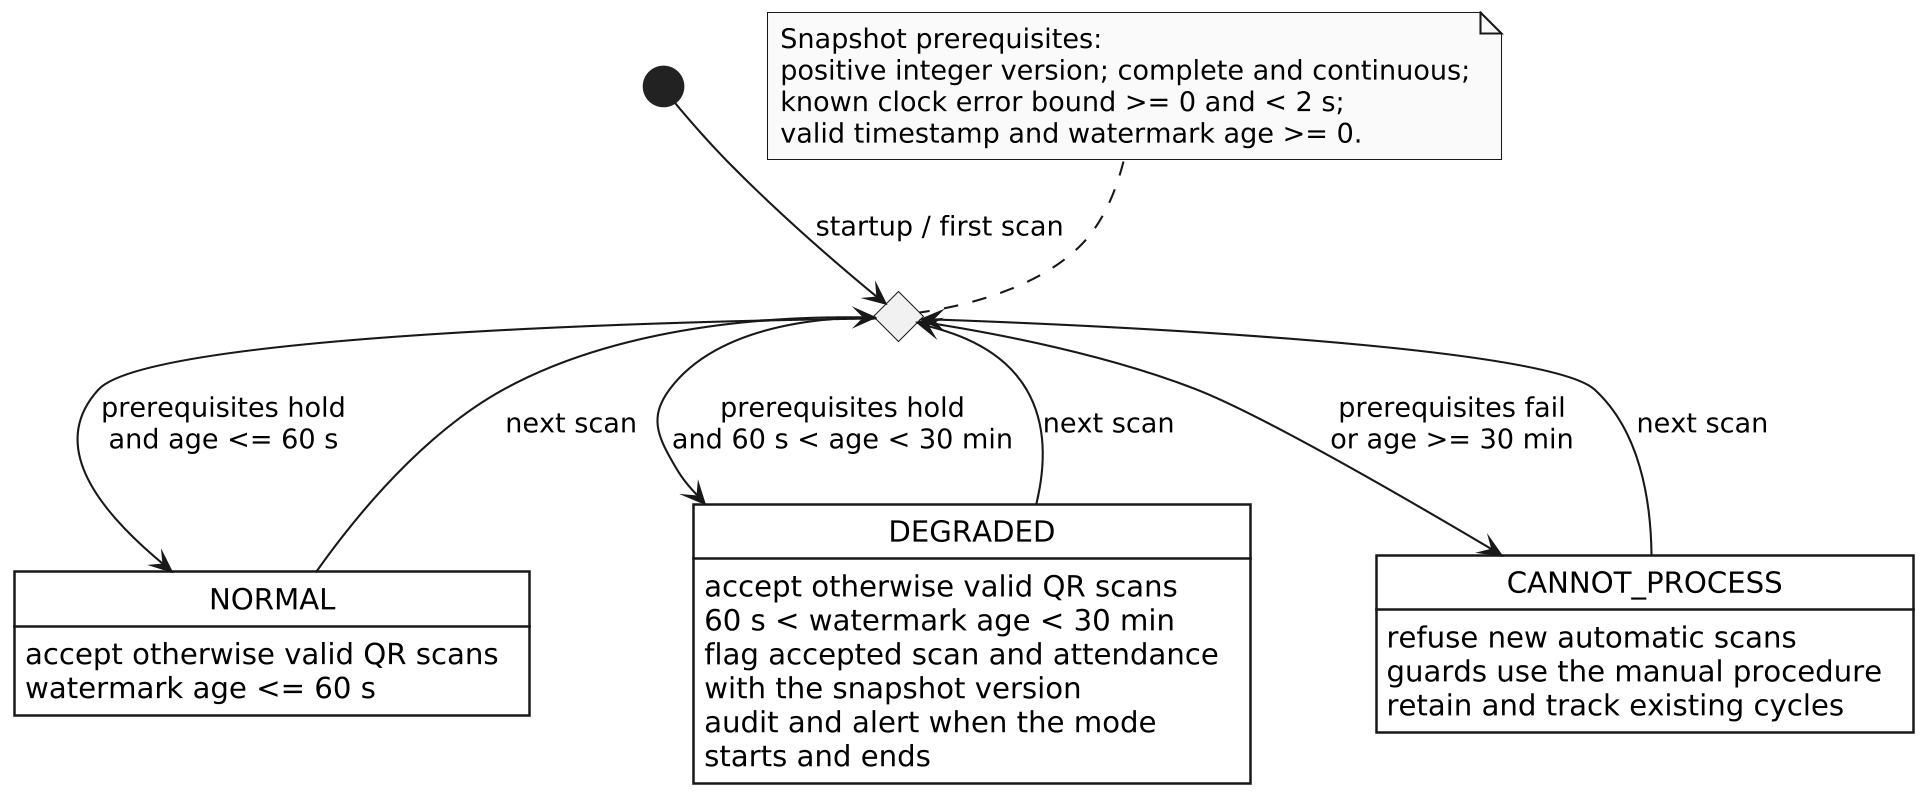
\includegraphics[width=0.9\linewidth]{diagram/deployment/figure-5-3-operating-modes.png}}{\fbox{\parbox{300pt}{\centering\vspace{20pt}Figure being redrawn\vspace{20pt}}}}

\vspace{6pt}
\textbf{Figure 5.3. Operating Modes of a Factory during Connectivity Loss}
\phantomsection\addcontentsline{lof}{figure}{\protect\numberline{5.3}Operating Modes of a Factory during Connectivity Loss}
\end{minipage}

\vspace{10pt}

Figure 5.3 shows the eligibility-mode decision made from the snapshot for every scan, including after restart. NORMAL requires a valid snapshot and a watermark at most 60 seconds old; a valid snapshot older than 60 seconds but younger than 30 minutes gives DEGRADED. Reconnection alone does not select NORMAL: the applied snapshot must meet those conditions. Storage failure is a separate reason to refuse a new opening even when the snapshot mode is NORMAL. CANNOT\_PROCESS does not itself authorize closing; existing cycles still follow the PASSAGE, LANE\_CLEAR, emergency, and durable-write rules. Audit and alerts on entry to and exit from DEGRADED are design requirements. The prototype emits these through in-memory stubs when it enters DEGRADED and returns to NORMAL; it does not emit an end event on transition to CANNOT\_PROCESS. In CANNOT\_PROCESS, guards use the approved manual procedure (Section 5.7.2).

\textbf{How the enhancements mitigate the issue.} Table 5.8 checks each concern from the problem statement against the enhancements and states the risk that remains.

\begin{longtable}{|>{\raggedright\arraybackslash}p{84pt}|>{\raggedright\arraybackslash}p{186pt}|>{\raggedright\arraybackslash}p{141pt}|}
\hline
\multicolumn{1}{|>{\columncolor{tableheader}\centering\arraybackslash}p{84pt}|}{\textbf{Concern}} & \multicolumn{1}{>{\columncolor{tableheader}\centering\arraybackslash}p{186pt}|}{\textbf{Result with E1--E5}} & \multicolumn{1}{>{\columncolor{tableheader}\centering\arraybackslash}p{141pt}|}{\textbf{Remaining risk}} \\
\hline
\endhead
\multicolumn{3}{c}{\rule{0pt}{20pt}\normalsize\phantomsection\addcontentsline{lot}{table}{\protect\numberline{5.8}Mitigation of Connectivity Loss}\textbf{Table 5.8. Mitigation of Connectivity Loss}} \\
\endlastfoot
Lost attendance record & The record and its outbox event are committed at the factory before anything is sent to the central site, and they are delivered later with the same eventId. & The outbox must be large enough for the outage (sized for 48 hours, alerts at 70\% and 85\%, Table 5.5). \\
\hline
Duplicate record & scanId, tokenId, passageEventId, and eventId are each unique, and central consumers use eventId and version to skip events they have already processed. & Missing versions and the outbox backlog have to be monitored (ADR-05). \\
\hline
Gate state unknown & An uncertain opening is queried where the controller supports it and otherwise reconciled, never resent, and the lane stays held until the outcome is known. & A held lane may need a guard to step in during the shift peak. \\
\hline
Out-of-date access rights & Degraded mode lasts less than 30 minutes, and every scan in it is flagged with its snapshot version for Attendance Review. & A revoked employee can still pass during that window, and the flag cannot undo the entry (I-10). \\*
\hline\noalign{\nobreak}
Central site down & Automatic scans stop within about 60 seconds as the shown codes expire, and the manual procedure takes over. & Guard staffing for about 80 arrivals per minute at the peak (Section 5.7.2). \\
\hline
\end{longtable}

\textbf{Example: the opening reply is lost.} Scan S-1 on LANE-BD-01 passes the checks, and ACCEPTED, the token claim, the gate cycle, and the OPEN command are committed in one transaction. The controller may now open the gate, but its reply does not arrive within the time left. Gate Core stores UNDETERMINED and keeps the lane and the token held. If a supported status query returns OPEN\_CONFIRMED, Gate Core records OPENED. Confirmed non-execution produces CONTROLLER\_ERROR. If no query is available or the outcome remains unknown, the scan moves to PENDING\_RECONCILIATION. Gate Core does not resend the OPEN command.

\textbf{What the prototype shows.} The Task 2 code covers E2, E3, and the mode rules of E4 for one factory (Chapter 9). Tests on a real SQLite file show that an UNDETERMINED opening becomes PENDING\_RECONCILIATION without a second openGate, that a controller signal sent twice still gives one attendance record, and that the stored state survives an application restart (\code{test_e2e_sqlite_flows.py}). The NORMAL, DEGRADED, and CANNOT\_PROCESS limits are tested in \code{test_pkg1_snapshot.py}. Site Sync, the broker, and the central site are not built, so delivery after reconnection (E5) is shown only in the design.

\Needspace{9\baselineskip}
\subsubsection*{5.8.2. Exposure of a Static QR Code}

\phantomsection
\addcontentsline{toc}{subsubsection}{5.8.2. Exposure of a Static QR Code}

\textbf{Problem.} A static QR code never changes. Anyone who gets a photo, a screenshot, or a forwarded copy of it can pass the gate and create attendance in the employee's name for as long as the code is accepted, and the system cannot tell the copy from the original. Table 5.9 lists the ways a code can be misused.

\begin{longtable}{|>{\raggedright\arraybackslash}p{40pt}|>{\raggedright\arraybackslash}p{120pt}|>{\raggedright\arraybackslash}p{251pt}|}
\hline
\multicolumn{1}{|>{\columncolor{tableheader}\centering\arraybackslash}p{40pt}|}{\textbf{ID}} & \multicolumn{1}{>{\columncolor{tableheader}\centering\arraybackslash}p{120pt}|}{\textbf{Threat}} & \multicolumn{1}{>{\columncolor{tableheader}\centering\arraybackslash}p{251pt}|}{\textbf{Example}} \\
\hline
\endhead
\multicolumn{3}{c}{\rule{0pt}{20pt}\normalsize\phantomsection\addcontentsline{lot}{table}{\protect\numberline{5.9}Threats from an Exposed QR Code}\textbf{Table 5.9. Threats from an Exposed QR Code}} \\
\endlastfoot
T1 & Copy used later & A colleague keeps a photo of the code and checks in for the employee the next day. \\
\hline
T2 & Copy used at the same time & The same image is shown at two lanes of one factory within a few seconds. \\
\hline
T3 & Copy used at the other factory & A code issued for Binh Duong is shown at Long An. \\
\hline
T4 & Forged or changed code & Someone edits the employee identifier inside the code or builds a new code. \\
\hline
T5 & Leak through a shared channel & A QR image sent by email is forwarded or stays in a mailbox. \\*
\hline\noalign{\nobreak}
T6 & Live sharing & The employee sends a fresh code to a colleague, who scans it before it expires. \\
\hline
\end{longtable}

\textbf{Alternatives considered.} Table 5.10 compares the options we looked at.

\begin{longtable}{|>{\raggedright\arraybackslash}p{110pt}|>{\raggedright\arraybackslash}p{140pt}|>{\raggedright\arraybackslash}p{161pt}|}
\hline
\multicolumn{1}{|>{\columncolor{tableheader}\centering\arraybackslash}p{110pt}|}{\textbf{Option}} & \multicolumn{1}{>{\columncolor{tableheader}\centering\arraybackslash}p{140pt}|}{\textbf{Strength}} & \multicolumn{1}{>{\columncolor{tableheader}\centering\arraybackslash}p{161pt}|}{\textbf{Weakness}} \\
\hline
\endhead
\multicolumn{3}{c}{\rule{0pt}{20pt}\normalsize\phantomsection\addcontentsline{lot}{table}{\protect\numberline{5.10}Alternatives for Protecting the QR Credential}\textbf{Table 5.10. Alternatives for Protecting the QR Credential}} \\
\endlastfoot
Keep the static code and revoke it when a leak is reported & Nothing changes for employees. & A leak is rarely noticed, so revocation comes after the damage. \\
\hline
Static code plus a PIN at the kiosk & Adds a second factor. & Typing a PIN slows the shift-change peak, and a PIN can be shared as easily as the image. \\
\hline
Code that changes on the phone from a shared secret (TOTP style) & Works without a network on the phone. & The secret must be stored on every phone and at every factory, and a leaked secret lets anyone build valid codes. \\
\hline
Short-lived code signed at the central site, bound to one factory and used once (chosen) & The private key stays at the central site, factories need only public keys, and a code is useless after 60 seconds or after its first claim. & The phone needs to reach the central site to get a code, and the code still does not prove who holds the phone. \\
\hline
Code signed by a key kept in the employee's phone & Ties the code to one registered phone. & Needs a device enrollment process and the mobile app on every phone, and does not stop an employee from handing over the phone. \\*
\hline\noalign{\nobreak}
Guard or biometric check of the person at the gate & Checks the person who holds the code. A badge alone would only add another credential that can be lent. & New hardware or extra guard work, slower lanes, and extra personal data to protect (NFR-04). Outside the scope of this design. \\
\hline
\end{longtable}

\textbf{Chosen enhancement.} We use the short-lived signed code of ADR-11 and I-09. QR Credential Issuance at the central site signs a code that holds the token identifier, the employee identifier, the factory, and its validity, and that expires 60 seconds after it is issued. Access Decision at the factory checks the signature with the public key, the validity period, the factory, and the employee's rights in Eligibility Snapshot. Gate Transaction Processor then claims the tokenId in the same transaction as ACCEPTED, so only one scan across all lanes of the factory can use it (Section 7.3). Under assumption I-08, company email only links to the live code screen and never carries a reusable image. Attendance is still created only from a timely PASSAGE linked to a scan that is still OPENED, not from the scan or the opening alone; an emergency-superseded or late passage is retained for review.

\textbf{How the enhancement mitigates the issue.} Table 5.11 maps each threat to the control that stops it and to the risk that is left.

\begin{longtable}{|>{\raggedright\arraybackslash}p{28pt}|>{\raggedright\arraybackslash}p{220pt}|>{\raggedright\arraybackslash}p{163pt}|}
\hline
\multicolumn{1}{|>{\columncolor{tableheader}\centering\arraybackslash}p{28pt}|}{\textbf{ID}} & \multicolumn{1}{>{\columncolor{tableheader}\centering\arraybackslash}p{220pt}|}{\textbf{Control}} & \multicolumn{1}{>{\columncolor{tableheader}\centering\arraybackslash}p{163pt}|}{\textbf{Remaining risk}} \\
\hline
\endhead
\multicolumn{3}{c}{\rule{0pt}{20pt}\normalsize\phantomsection\addcontentsline{lot}{table}{\protect\numberline{5.11}Mitigation of QR Exposure}\textbf{Table 5.11. Mitigation of QR Exposure}} \\
\endlastfoot
T1 & The code expires after 60 seconds, and a claimed tokenId cannot be claimed again, so an old copy is rejected as expired or as a replay. & None after the code has expired or been claimed. \\
\hline
T2 & The claim is part of the ACCEPTED write and is protected by a unique key, so the second scan is rejected and audited. & The first scan wins, and it may be the copy. \\
\hline
T3 & The factory is part of the signed content and is compared with the server's own factory, not with a value sent by the kiosk. & None. \\
\hline
T4 & Any change breaks the signature, and only the central site holds the private key. & Theft of the private key at the central site. \\
\hline
T5 & No reusable image is sent; email only links to the authenticated live display. & I-08 is still an assumption that TMC has to confirm. \\*
\hline\noalign{\nobreak}
T6 & Not blocked. Attendance needs a real passage, and each scan is audited with its lane and time. & A valid, unclaimed copy may win the first scan. If TMC cannot accept this, an independent check of the person at the gate is needed; device binding alone does not prevent sharing a displayed code. \\
\hline
\end{longtable}

\textbf{Example: one image at two lanes.} An employee scans a valid code at LANE-BD-01, and a few seconds later a photo of the same code is shown at LANE-BD-02. The first scan claims the tokenId in the same transaction as ACCEPTED, so the second one is stored as REJECTED with QR\_TOKEN\_REPLAY\_DETECTED and audited with its lane and time. The order could also be the other way round. Whichever accepted scan claims the token first wins. Reuse of that token is rejected, but the stored evidence does not establish who presented it.

\textbf{What the prototype shows.} The Task 2 code verifies the factory side of this enhancement with real Ed25519 keys: signature, expiry, factory binding, and key rotation in \code{test_pkg2_*.py}, two connections claiming one token in \code{test_pkg4_sqlite_repos.py}, and a copied code on another lane rejected with QR\_TOKEN\_REPLAY\_DETECTED in \code{test_e2e_sqlite_flows.py}. The QR issuer in the prototype is only a demo helper, not the central issuing service.

\Needspace{9\baselineskip}
\subsubsection*{5.8.3. Impact on the Architecture}

\phantomsection
\addcontentsline{toc}{subsubsection}{5.8.3. Impact on the Architecture}

Neither enhancement needs a new module or node. They are rules inside modules that already exist, fixed by ADR-02, ADR-05, ADR-06, and ADR-11. Table 5.12 shows where each part lives.

\begin{longtable}{|>{\raggedright\arraybackslash}p{95pt}|>{\raggedright\arraybackslash}p{316pt}|}
\hline
\multicolumn{1}{|>{\columncolor{tableheader}\centering\arraybackslash}p{95pt}|}{\textbf{Module or node}} & \multicolumn{1}{>{\columncolor{tableheader}\centering\arraybackslash}p{316pt}|}{\textbf{Role in the two enhancements}} \\
\hline
\endhead
\multicolumn{2}{c}{\rule{0pt}{20pt}\normalsize\phantomsection\addcontentsline{lot}{table}{\protect\numberline{5.12}Where the Enhancements Live}\textbf{Table 5.12. Where the Enhancements Live}} \\
\endlastfoot
M1 Gate Core (factory) & Access Decision checks the signed code and the operating mode; Gate Transaction Processor stores ACCEPTED and the token claim before openGate, handles uncertain results without resending, and writes attendance with its outbox event. \\
\hline
M2 Turnstile Integration (factory) & Queries the controller about uncertain commands where supported; otherwise Gate Core retains the uncertain outcome for reconciliation. \\
\hline
M4 Access \& Configuration (central) & QR Credential Issuance signs short-lived codes and keeps the private key; the Access Change Feed sends access rights and confirmed watermarks to the factories. \\
\hline
M9 Site Sync (both sites) & Delivers outbox events with their original identifiers and applies access-right updates in the recovery order of Figure 5.2. \\
\hline
M5 Attendance (central) & Attendance Review checks DEGRADED transactions after reconnection and handles reconciliation cases. \\
\hline
M11 Audit, M12 Monitoring & Record rejected replays and the start and end of degraded mode, and raise alerts for degraded mode and outbox capacity. \\
\hline
Factory server and database & Primary and standby with a synchronous copy (Section 5.6.2), so a server failure does not lose the token claims or the outbox. \\*
\hline\noalign{\nobreak}
Central reverse proxy and broker & The proxy runs as an active/standby pair because QR issuing depends on it; the broker has a recovery target that stays below the 30-minute limit (Table 5.5). \\
\hline
\end{longtable}


\newpage
% ==================== CHAPTER 6 ====================
\section*{6. ARCHITECTURE DECISIONS}

\phantomsection
\addcontentsline{toc}{section}{6. ARCHITECTURE DECISIONS}

This chapter records the main design decisions, the reasons behind them, and what they cost.

\Needspace{9\baselineskip}
\subsection*{6.1. Decision Log}

\phantomsection
\addcontentsline{toc}{subsection}{6.1. Decision Log}


Table 6.1 lists the eleven decisions. All of them rely on the API assumptions in Table 1.1.

\begin{longtable}{|>{\raggedright\arraybackslash}p{46pt}|>{\raggedright\arraybackslash}p{381pt}|}
\hline
\multicolumn{1}{|>{\columncolor{tableheader}\centering\arraybackslash}p{46pt}|}{\textbf{ID}} & \multicolumn{1}{>{\columncolor{tableheader}\centering\arraybackslash}p{381pt}|}{\textbf{Decision}} \\
\hline
\endhead
\multicolumn{2}{c}{\rule{0pt}{20pt}\normalsize\textbf{Table 6.1. TMC Architecture Decision Log}} \\
\endlastfoot
ADR-01 & Use Service-based Architecture with Event-driven Integration, and organize the modules within each application as a Modular Monolith. \\
\hline
ADR-02 & Persist the accepted scan before opening; distinguish command receipt, confirmed opening, passage, and closing. Create automatic attendance only after a passage event. \\
\hline
ADR-03 & Assign data ownership to individual modules and use public interfaces for communication between modules. \\
\hline
ADR-04 & Isolate controller and HR/Payroll integration through two ports and their corresponding adapters. \\
\hline
ADR-05 & Transfer events persisted at the source, with duplicate-safe processing and tracking of application results. \\
\hline
ADR-06 & Use Eligibility Snapshot at each factory; after 60 seconds without confirmed updates, continue in a flagged degraded mode while the last confirmed update is less than 30 minutes old. \\
\hline
ADR-07 & Separate support-case intake, approval, and application of decisions to attendance data. \\
\hline
ADR-08 & Perform batch-based HR/Payroll handover outside the gate-processing flow; track individual batch acknowledgements and completeness of the entire period separately. \\
\hline
ADR-09 & Enforce permissions by operation and data scope; retain audit evidence at the source and protect personal data across all copies. \\
\hline
ADR-10 & Use synchronous standby replication and separate backups; perform controlled failover without bypassing durability requirements during failures. \\*
\hline\noalign{\nobreak}
ADR-11 & Use signed QR credentials valid for 60 seconds, bound to one factory and claimable by one accepted scan. \\
\hline
\end{longtable}
\phantomsection\addcontentsline{lot}{table}{\protect\numberline{6.1}TMC Architecture Decision Log}


\subsection*{6.2. Architecture Decision Records}

\phantomsection
\addcontentsline{toc}{subsection}{6.2. Architecture Decision Records}

Each record below gives the characteristics involved, the context, the decision, the reasons, the consequences, and the trade-off.

\subsubsection*{6.2.1. ADR-01: Use Service-based Architecture with Event-driven Integration}

\phantomsection
\addcontentsline{toc}{subsubsection}{6.2.1. ADR-01: Use Service-based Architecture with Event-driven Integration}

\begin{itemize}[leftmargin=36pt, itemsep=2pt, topsep=4pt, parsep=2pt]
  \item \textbf{Characteristics:} AC-01, AC-02, AC-03.
  \item \textbf{Context:} Both factories need a kiosk result within 2 seconds and must keep scanning when their WAN link fails, while consolidation, reporting, and handover can run minutes or hours later.
  \item \textbf{Decision:} Each factory runs its own gate application and database, and the central site runs one application for access data, attendance, reports, and handover. Three event feeds carry gate records, access changes, and resolutions between them. Inside each application, the modules form a Modular Monolith.
  \item \textbf{Reasons:} QR validation, durable recording, and the controller call stay on the factory LAN, so the WAN is not on the scan path and a fault at one factory does not stop the other. Microservices or a broker on the gate path would add network hops without any benefit at this load.
  \item \textbf{Consequences:} TMC has to run applications and databases at three sites and keep event contracts compatible across them.
  \item \textbf{Trade-off:} We give up the simplicity of one deployment and accept that central data lags behind the gates. Scanning during a WAN outage is limited by ADR-06.
\end{itemize}

\subsubsection*{6.2.2. ADR-02: Persist Accepted Scans and Record Attendance after Passage}

\phantomsection
\addcontentsline{toc}{subsubsection}{6.2.2. ADR-02: Persist Accepted Scans and Record Attendance after Passage}

\begin{itemize}[leftmargin=36pt, itemsep=2pt, topsep=4pt, parsep=2pt]
  \item \textbf{Characteristics:} AC-01, AC-03, AC-05, AC-06.
  \item \textbf{Context:} The controller and the database are separate systems. A command receipt, a confirmed opening, a passage, and a closing are different facts, and an open gate does not prove that anyone passed.
  \item \textbf{Decision:} Store ACCEPTED and the token claim before openGate. Report a confirmed opening only after OPEN\_CONFIRMED is stored. Create one automatic attendance transaction only after a linked passage event (I-07). Send closeGate after LANE\_CLEAR and record CLOSED only when the controller confirms it (I-05).
  \item \textbf{Reasons:} If something fails after the command, the stored scan state shows what has happened, so recovery never has to guess. Attendance follows passage rather than the opening signal, so an opened but unused gate creates no record.
  \item \textbf{Consequences:} A repeated scanId returns its stored result. An uncertain command is inquired or reconciled and never resent automatically (I-03).
  \item \textbf{Trade-off:} The flow needs more states and more controller signals, and the signals in I-01 and I-05 still have to be verified with the vendor.
\end{itemize}

\subsubsection*{6.2.3. ADR-03: Assign Data Ownership to Modules and Use Public Interfaces}

\phantomsection
\addcontentsline{toc}{subsubsection}{6.2.3. ADR-03: Assign Data Ownership to Modules and Use Public Interfaces}

\begin{itemize}[leftmargin=36pt, itemsep=2pt, topsep=4pt, parsep=2pt]
  \item \textbf{Characteristics:} AC-01, AC-04; Maintainability.
  \item \textbf{Context:} Attendance, Reporting, and Payroll Handover use related data, but for different work and under different rules.
  \item \textbf{Decision:} Each module writes only its own data. Other modules use its public interface, even when they share a database engine; Reporting and Payroll Handover, for example, read attendance through AttendanceApi.
  \item \textbf{Reasons:} Business rules and schema changes stay with the module that owns them, and permission checks happen in one place.
  \item \textbf{Consequences:} Contracts must define data, versions, and errors, and code review must check that no module reads another module's tables.
  \item \textbf{Trade-off:} Interfaces add mapping work, but direct table access would spread dependencies across the system.
\end{itemize}

\subsubsection*{6.2.4. ADR-04: Isolate External Systems through Ports and Adapters}

\phantomsection
\addcontentsline{toc}{subsubsection}{6.2.4. ADR-04: Isolate External Systems through Ports and Adapters}

\begin{itemize}[leftmargin=36pt, itemsep=2pt, topsep=4pt, parsep=2pt]
  \item \textbf{Characteristics:} AC-01, AC-03, AC-06.
  \item \textbf{Context:} The controller and HR/Payroll APIs have their own formats, and the meaning of their responses is not fully specified.
  \item \textbf{Decision:} Gate Core defines the command ports grouped as ITurnstileControl and the separate event port IPassageEvents. Turnstile Adapter implements the command ports, and Gate Core implements IPassageEvents, which the adapter calls for PASSAGE and LANE\_CLEAR. Payroll Handover defines IPayrollSubmission, implemented by HR/Payroll Adapter.
  \item \textbf{Reasons:} Business code works with clear meanings such as ``opening confirmed'' or ``outcome unknown'' instead of vendor response codes, and an API change stays inside one adapter.
  \item \textbf{Consequences:} An adapter never turns a command receipt into a confirmed opening, and opening, passage, and closing stay separate. The API capabilities in I-01, I-02, and I-05 still need verification.
  \item \textbf{Trade-off:} Adapters need contract tests, and they cannot create signals that the external systems do not provide.
\end{itemize}

\subsubsection*{6.2.5. ADR-05: Deliver Persisted Events with Duplicate-safe Processing}

\phantomsection
\addcontentsline{toc}{subsubsection}{6.2.5. ADR-05: Deliver Persisted Events with Duplicate-safe Processing}

\begin{itemize}[leftmargin=36pt, itemsep=2pt, topsep=4pt, parsep=2pt]
  \item \textbf{Characteristics:} AC-01, AC-02, AC-05.
  \item \textbf{Context:} Factory events must survive WAN and broker outages, and they may be delivered twice or out of order.
  \item \textbf{Decision:} Store each business change and its outgoing event together in an outbox. Consumers store the change and an event-processed marker together and use eventId and version to skip duplicates and stale data.
  \item \textbf{Reasons:} An event is never lost because it is saved at the source first, and delivering it again later does no harm.
  \item \textbf{Consequences:} Missing versions and outbox backlog must be monitored. A broker receipt does not prove that the business change was applied.
  \item \textbf{Trade-off:} Central data may lag behind the factories. Event deduplication does not replace the per-scan and QR replay checks.
\end{itemize}

\subsubsection*{6.2.6. ADR-06: Use Local Eligibility Data with a Bounded Degraded Mode}

\phantomsection
\addcontentsline{toc}{subsubsection}{6.2.6. ADR-06: Use Local Eligibility Data with a Bounded Degraded Mode}

\begin{itemize}[leftmargin=36pt, itemsep=2pt, topsep=4pt, parsep=2pt]
  \item \textbf{Characteristics:} AC-02, AC-04.
  \item \textbf{Context:} Checking access at the central site for every scan would put the WAN on the scan path, but a local copy may miss a recent revocation.
  \item \textbf{Decision:} Access Decision uses the factory's Eligibility Snapshot while its completeness, version, continuity, and freshness checks pass. The data is fresh for 60 seconds after a source-confirmed watermark. After that, Gate Core runs in degraded mode while the same watermark is less than 30 minutes old, accepts only valid signed QR codes, and flags every transaction for review (I-10). From 30 minutes on, new scans return CANNOT PROCESS.
  \item \textbf{Reasons:} The local copy keeps the scan off the WAN, and the degraded window keeps the gates working through one shift-change peak when the link fails.
  \item \textbf{Consequences:} New automatic scans stop when the limit is reached or data continuity is lost, and Attendance Review checks the flagged transactions after reconnection. QR validity and replay control are handled separately by ADR-11.
  \item \textbf{Trade-off:} A revocation may remain unknown until reconnection. The 30-minute watermark limit bounds how long automatic acceptance can use old rights; it does not guarantee delivery within 30 minutes. TMC must approve both limits; immediate revocation would need an online check or stopping the affected scans.
\end{itemize}

\subsubsection*{6.2.7. ADR-07: Separate Assisted Access Approval from Attendance Application}

\phantomsection
\addcontentsline{toc}{subsubsection}{6.2.7. ADR-07: Separate Assisted Access Approval from Attendance Application}

\begin{itemize}[leftmargin=36pt, itemsep=2pt, topsep=4pt, parsep=2pt]
  \item \textbf{Characteristics:} AC-01, AC-04, AC-05.
  \item \textbf{Context:} Helping an employee at the gate, approving the case, and changing attendance are different actions done by different people.
  \item \textbf{Decision:} Gate Intervention records and authorizes an eligible assisted opening through Gate Core. Attendance Review manages the evidence and HR approval, and Attendance Consolidation applies the approved decision. A case linked to a scan also sends its resolution to Gate Core through Resolution Feed.
  \item \textbf{Reasons:} A guard's action alone cannot create attendance (I-04), and each step leaves its own evidence.
  \item \textbf{Consequences:} Attendance Review tracks whether each decision has been applied in Attendance and, when needed, in Gate Core, using decision identifiers and versions.
  \item \textbf{Trade-off:} The workflow adds states and delay. Emergency release stays a separate authorized action and never creates attendance.
\end{itemize}

\subsubsection*{6.2.8. ADR-08: Track Monthly HR/Payroll Handover by Batch and Period}

\phantomsection
\addcontentsline{toc}{subsubsection}{6.2.8. ADR-08: Track Monthly HR/Payroll Handover by Batch and Period}

\begin{itemize}[leftmargin=36pt, itemsep=2pt, topsep=4pt, parsep=2pt]
  \item \textbf{Characteristics:} AC-01, AC-06.
  \item \textbf{Context:} Factory events and approvals may arrive late, and a lost HR/Payroll response leaves receipt uncertain.
  \item \textbf{Decision:} Payroll Handover stores batch content and identity before submission, confirms receipt under I-02, and tracks the completeness of the whole period separately. The first submission is planned for 06:00, with an alert at 10:00 and linked supplementary batches before noon where needed.
  \item \textbf{Reasons:} One confirmed batch may cover only part of the period, so batch receipt and period completion cannot be the same flag.
  \item \textbf{Consequences:} An uncertain batch is checked by status inquiry where the API supports it. It is resent only when the contract prevents duplicates or evidence shows that resending is safe; otherwise an alert is raised.
  \item \textbf{Trade-off:} Batch and period tracking adds work, and a long outage of a source or of HR/Payroll can still miss the deadline.
\end{itemize}

\subsubsection*{6.2.9. ADR-09: Enforce Scoped Access and Preserve Auditable, Minimal Data}

\phantomsection
\addcontentsline{toc}{subsubsection}{6.2.9. ADR-09: Enforce Scoped Access and Preserve Auditable, Minimal Data}

\begin{itemize}[leftmargin=36pt, itemsep=2pt, topsep=4pt, parsep=2pt]
  \item \textbf{Characteristics:} AC-04, AC-05.
  \item \textbf{Context:} Six user groups have different authority, and personal and audit data is copied across sites and backups.
  \item \textbf{Decision:} Check identity, operation, and data scope at the server for every request. Store audit evidence at its source and send it to Audit Log; Reporting checks authorization before calling AuditApi.query. Keep personal data out of tokens, displays, events, and logs unless it is needed.
  \item \textbf{Reasons:} A direct API call faces the same checks as the user interface, and evidence stored at the source survives an interrupted transfer.
  \item \textbf{Consequences:} Access and retention rules apply to every copy of the data, including backups. Chapter 7 describes audit content and data protection.
  \item \textbf{Trade-off:} Traceability needs data to be kept, while privacy limits how much is kept and for how long.
\end{itemize}

\Needspace{10\baselineskip}
\subsubsection*{6.2.10. ADR-10: Use Controlled Failover with Synchronous Replication and Separate Backups}

\phantomsection
\addcontentsline{toc}{subsubsection}{6.2.10. ADR-10: Use Controlled Failover with Synchronous Replication and Separate Backups}

\begin{itemize}[leftmargin=36pt, itemsep=2pt, topsep=4pt, parsep=2pt]
  \item \textbf{Characteristics:} AC-01, AC-02, AC-03.
  \item \textbf{Context:} A standby covers hardware failures, but a deletion or corruption is copied to the standby as well.
  \item \textbf{Decision:} Use a primary and a standby database at each factory, two central application instances, synchronous database replication, and separate backups. Isolate the former primary before a replacement accepts writes or sends commands. A commit is acknowledged only when the durability conditions are met.
  \item \textbf{Reasons:} Replication protects acknowledged commits when one database fails, and backups cover the failures that replication copies.
  \item \textbf{Consequences:} New scans stop if safe durable writes are not possible, and recovery checks unfinished scans and token claims before scanning restarts.
  \item \textbf{Trade-off:} Cost and write latency increase. The recovery targets in Chapter 5 are proposals that still have to be measured.
\end{itemize}

\subsubsection*{6.2.11. ADR-11: Use Short-lived, Factory-bound QR Credentials}

\phantomsection
\addcontentsline{toc}{subsubsection}{6.2.11. ADR-11: Use Short-lived, Factory-bound QR Credentials}

\begin{itemize}[leftmargin=36pt, itemsep=2pt, topsep=4pt, parsep=2pt]
  \item \textbf{Characteristics:} AC-01, AC-04, AC-06.
  \item \textbf{Context:} A reusable QR image can be copied and shown by another person.
  \item \textbf{Decision:} Under I-09, the central site issues a signed QR credential valid for 60 seconds and bound to one factory. All lanes of that factory share Gate Core's token-claim data, and one tokenId is claimed by only one ACCEPTED scan, in the same write as ACCEPTED and before openGate.
  \item \textbf{Reasons:} The short lifetime, the factory binding, and the shared claim limit reuse without a central call for each scan.
  \item \textbf{Consequences:} Chapter 7 describes issuance, validation, and replay control. The email route to the QR display is still an assumption (I-08).
  \item \textbf{Trade-off:} A copied image can still be used before its first claim, because the credential alone does not prove who is holding the phone.
\end{itemize}

\Needspace{15\baselineskip}
\subsection*{6.3. Mapping ADRs to Requirements and Architecture Views}

\phantomsection
\addcontentsline{toc}{subsection}{6.3. Mapping ADRs to Requirements and Architecture Views}


Table 6.2 links each decision to the requirements it supports and the sections where it appears in the design. A requirement listed for one ADR may also need other decisions to be met in full.

External API capabilities, replay behavior after recovery, and TMC's approval of the two eligibility-data limits (I-10) are still open and are listed in Section 10.2.

\begin{longtable}{|>{\raggedright\arraybackslash}p{41.5pt}|>{\raggedright\arraybackslash}p{145.5pt}|>{\raggedright\arraybackslash}p{224.5pt}|}
\hline
\multicolumn{1}{|>{\columncolor{tableheader}\centering\arraybackslash}p{41.5pt}|}{\textbf{ADR}} & \multicolumn{1}{>{\columncolor{tableheader}\centering\arraybackslash}p{145.5pt}|}{\textbf{Related requirements and supporting basis}} & \multicolumn{1}{>{\columncolor{tableheader}\centering\arraybackslash}p{224.5pt}|}{\textbf{Corresponding view or design section}} \\
\hline
\endhead
\multicolumn{3}{c}{\rule{0pt}{20pt}\normalsize\textbf{Table 6.2. Mapping ADRs to Requirements and Architecture}} \\
\endlastfoot
ADR-01 & NFR-01; operation at two factories; AC-02 & Selection analysis in Sections 3.3--3.5; application placement and component mapping in Section 5.2. \\
\hline
ADR-02 & FR-02.2; FR-03.3--FR-03.6; NFR-01; NFR-02; NFR-03; I-01; I-03; I-05; I-07 & QR flow in Section 4.2.2; states and processing order in Section 4.2.5; durable persistence in Section 5.6.1. \\
\hline
ADR-03 & FR-04.1--FR-04.4; FR-04.6--FR-04.7; NFR-03; NFR-04 & Module View and dependency rules in Section 4.1; data ownership in Section 4.2.1; central data persistence in Section 5.6.1. \\
\hline
ADR-04 & FR-02.2; FR-04.3; IC-01; IC-02; I-01--I-03; I-05 & The two ports in the Module View and C\&C View; contracts in Section 4.2.1; external-system connections in Section 5.3. \\
\hline
ADR-05 & FR-03.3--FR-03.6; FR-04.4--FR-04.5; NFR-02; NFR-03 & Channels in the C\&C View; duplicate prevention in Section 4.2.5; Event-driven Integration in Section 3.5; delivery and acknowledgement in Section 5.3. \\
\hline
ADR-06 & FR-01.4; FR-03.2; NFR-03; AC-02; AC-04 & Eligibility Snapshot in Sections 4.1.1 and 4.2.5; conditions for using access-right data in Sections 5.7.2--5.7.3. \\
\hline
ADR-07 & FR-03.3; FR-04.4--FR-04.5; NFR-03; I-04 & Support flow and decision application in Section 4.2.3; support and emergency handling in Section 5.7.4. \\
\hline
ADR-08 & FR-04.2--FR-04.3; IC-01; I-02 & Handover flow in Section 4.2.4; batch states in Section 4.2.5; handover recovery in Section 5.7.4. \\
\hline
ADR-09 & FR-04.5--FR-04.7; FR-05.1; FR-05.5; NFR-03; NFR-04 & Authorization and audit in Section 4.2.1; network, access, and data boundaries in Section 5.5. \\
\hline
ADR-10 & FR-02.3; FR-05.3--FR-05.4; NFR-01; NFR-02; AC-02 & Deployment View in Section 5.1; standby replication and backups in Sections 5.6.2--5.6.3; recovery and verification in Section 5.7. \\*
\hline\noalign{\nobreak}
ADR-11 & FR-01.2--FR-01.3; FR-03.2; NFR-03; I-08--I-09 & QR issuance, validation, and replay controls in Sections 7.3.1--7.3.3; response to Issue 2 in Section 5.8.2. \\
\hline
\end{longtable}
\phantomsection\addcontentsline{lot}{table}{\protect\numberline{6.2}Mapping ADRs to Requirements and Architecture}


\newpage
% ==================== CHAPTER 7 ====================
\section*{7. DESIGN PRINCIPLES AND DATA SECURITY}

\phantomsection
\addcontentsline{toc}{section}{7. DESIGN PRINCIPLES AND DATA SECURITY}

This chapter shows how design principles keep the module boundaries of Chapter 4 clear, and how QR codes, permissions, audit records, and personal data are protected.

\subsection*{7.1. SOLID Principles}

\phantomsection
\addcontentsline{toc}{subsection}{7.1. SOLID Principles}

The modules own distinct decisions and data. Gate Core owns factory scan and passage records, Access \& Configuration owns access rights and station settings, Attendance owns consolidation and review, and Payroll Handover owns batches. Modules exchange data through public contracts, and the two external adapters implement ports defined by Gate Core and Payroll Handover. We apply SOLID to these modules, interfaces, and ports, not only to classes.

\subsubsection*{7.1.1. Single Responsibility Principle (SRP)}

\phantomsection
\addcontentsline{toc}{subsubsection}{7.1.1. Single Responsibility Principle (SRP)}

SRP says that a unit should have one cohesive responsibility and one kind of reason to change. It does not mean that a component may perform only one operation.

\textbf{In TMC:}

\begin{itemize}[leftmargin=36pt, itemsep=2pt, topsep=4pt, parsep=2pt]
  \item Gate Transaction Processor receives a scan, handles repeated requests, asks for the eligibility check, stores the accepted attempt, and coordinates opening, passage, and closing. All of these belong to one gate transaction; accounts, shift rules, and reports live elsewhere.
  \item Access Decision only decides eligibility. A change in how the controller is called belongs in Turnstile Adapter.
  \item Under I-06, shift rules affect Work Schedule Policy and attendance aggregation, not the gate decision. If TMC also wants shifts to restrict physical access, Access Decision needs an explicit access-policy rule, still separate from the QR signature check.
  \item Attendance Review manages cases and approval authority, while Attendance Consolidation applies the right decision version, prevents duplicates, and keeps links to the original data.
\end{itemize}

\textbf{Benefit:} a change to the approval workflow or to the controller does not force a rewrite of attendance aggregation or of the gate rules.

\subsubsection*{7.1.2. Open--Closed Principle (OCP)}

\phantomsection
\addcontentsline{toc}{subsubsection}{7.1.2. Open--Closed Principle (OCP)}

OCP aims to add new capabilities while leaving stable business logic alone. In TMC, the clearest extension points are the two external integrations.

\textbf{In TMC:}

\begin{itemize}[leftmargin=36pt, itemsep=2pt, topsep=4pt, parsep=2pt]
  \item A new controller that keeps the meaning of the turnstile ports (opening and closing results, passage and lane-clear events, emergency release and reset) only needs a new adapter, and the gate rules do not change.
  \item An HR/Payroll format change that keeps the meaning of IPayrollSubmission only changes HR/Payroll Adapter.
  \item Work Schedule Policy keeps shift and aggregation rules in one place, so a change that fits its configuration model is not implemented twice in Attendance and Reporting. A rule outside that model still needs code changes and tests.
\end{itemize}

\textbf{Limit:} OCP does not mean that code never changes. Since each application is a Modular Monolith, replacing an adapter may still need a new release of that application. The aim is that integration changes do not spread to unrelated components.

\subsubsection*{7.1.3. Liskov Substitution Principle (LSP)}

\phantomsection
\addcontentsline{toc}{subsubsection}{7.1.3. Liskov Substitution Principle (LSP)}

LSP says that a replacement must keep the behavior its consumers rely on; matching method names and types is not enough.

\Needspace{6\baselineskip}
\textbf{In TMC:} a replacement adapter must keep this behavior:

\begin{itemize}[leftmargin=36pt, itemsep=2pt, topsep=4pt, parsep=2pt]
  \item For the turnstile ports, a command receipt is not OPEN\_CONFIRMED. openGate returns only OPEN\_CONFIRMED, CONTROLLER ERROR when the controller explicitly confirms it did not open, or UNDETERMINED. Passage is a later event, LANE\_CLEAR allows closeGate, and only the controller's close confirmation means CLOSED. emergencyRelease succeeds only on EMERGENCY\_RELEASED, and resetEmergency only on RESET\_CONFIRMED. Both can instead return explicit CONTROLLER ERROR or UNDETERMINED; requesting reset alone never ends the hold. A timeout after the command may have been sent stays undetermined.
  \item Gate Core records automatic attendance only when the passage event of I-01 is received and stored. A controller without reliable passage evidence cannot satisfy I-07 by returning an opening confirmation.
  \item For IPayrollSubmission, a receipt acknowledgement (I-02) only proves that HR/Payroll received that batch. When every mandatory part of the period is in CONFIRMED batches, the handover is complete (Flow C). IC-01 also needs the data to be ready for reconciliation before noon, so either the acknowledgement contract must guarantee this or HR/Payroll must give separate evidence; this has to be agreed with its owner.
  \item Status queries are used only where the API supports them. If a controller lacks the passage or safe-closing behavior assumed in I-01 and I-05, the integration is revised, and reconciliation is used where automatic attendance cannot be justified.
\end{itemize}

\textbf{Benefit:} an adapter that passes the same contract tests can replace the old one without any change in Gate Core or Payroll Handover.

\Needspace{13\baselineskip}
\subsubsection*{7.1.4. Interface Segregation Principle (ISP)}

\phantomsection
\addcontentsline{toc}{subsubsection}{7.1.4. Interface Segregation Principle (ISP)}

ISP says that a consumer should depend only on the operations it uses.

\Needspace{6\baselineskip}
\textbf{In TMC:} the grouped interfaces in Table 4.20 are split into narrower design contracts:

\begin{itemize}[leftmargin=36pt, itemsep=2pt, topsep=4pt, parsep=2pt]
  \item \textbf{Turnstile ports:} Gate Core defines narrow contracts instead of one large interface. IOpenGate (openGate with a time limit), ICloseGate (closeGate), and IEmergencyGate (emergencyRelease and reset) are commands that return their results, and Turnstile Adapter implements them against the verified controller API (I-01, I-05). IPassageEvents (PASSAGE and LANE\_CLEAR) runs the other way: Gate Core implements it, and Turnstile Adapter calls it when the controller reports these events. Gate Transaction Processor uses the normal-cycle contracts, and the emergency coordinator uses IEmergencyGate. IControllerStatusQuery is a separate optional contract, used only where the controller API supports it.
  \item \textbf{GateCoreApi:} IScanSubmission for Station Client, IInterventionRequest for Gate Intervention (support case, assisted opening, emergency release and reset), and IFactoryUpdates for Site Sync.
  \item \textbf{Other APIs:} AttendanceApi separates review and approval from period-data queries, AuthorizationApi separates account administration from authorization checks, and AuditApi separates record intake from queries.
\end{itemize}

\textbf{Benefit:} each consumer sees only the operations it needs, so a change to one contract does not affect the other consumers.

\textbf{Limit:} these are design contracts, not a security control on their own. Server-side authorization still checks every operation and data scope.

\subsubsection*{7.1.5. Dependency Inversion Principle (DIP)}

\phantomsection
\addcontentsline{toc}{subsubsection}{7.1.5. Dependency Inversion Principle (DIP)}

Business code should depend on abstractions that it defines, not on the details of external systems.

\textbf{In TMC:}

\begin{itemize}[leftmargin=36pt, itemsep=2pt, topsep=4pt, parsep=2pt]
  \item Gate Transaction Processor depends on the command ports that Gate Core defines (IOpenGate, ICloseGate, IEmergencyGate), not on the Controller API format. Turnstile Adapter reports events back through IPassageEvents, which Gate Core also defines, so both directions point to Gate Core's abstractions.
  \item Gate Core also defines its storage ports. A unit-of-work port (IUnitOfWork) owns each transaction, so reserving the lane, claiming the token, and storing ACCEPTED happen in one write without Gate Transaction Processor knowing which database is used.
  \item Payroll Handover depends on IPayrollSubmission without knowing HR/Payroll connection details or response structures.
  \item Test adapters return command outcomes and deliver PASSAGE and LANE\_CLEAR through IPassageEvents. Receipt-only and timeout cases produce UNDETERMINED. A shared contract test suite checks substitution; integration tests check these meanings against the real controller.
\end{itemize}

\textbf{Limit:} not every internal call needs an interface. We add an abstraction only when it supports substitution, testing, or isolation of a real dependency.

\Needspace{9\baselineskip}
\subsection*{7.2. Cohesion, Coupling and Extensibility}

\phantomsection
\addcontentsline{toc}{subsection}{7.2. Cohesion, Coupling and Extensibility}

\subsubsection*{7.2.1. High Cohesion}

\phantomsection
\addcontentsline{toc}{subsubsection}{7.2.1. High Cohesion}


Functions belong in the same module when they serve related responsibilities:

\begin{itemize}[leftmargin=36pt, itemsep=2pt, topsep=4pt, parsep=2pt]
  \item Gate Core concentrates on scan processing at a factory, Attendance on recording, review, and aggregation, and Payroll Handover on preparing data and tracking its delivery.
  \item Inside a module, components keep distinct responsibilities. Access \& Configuration manages several kinds of business data, but QR issuance, access rights, stations, and shift policy are separate components.
  \item Modules are not built around data entities. There is no ``Employee module'': employee data is used in several places, but access decisions, aggregation, and account administration change for different reasons.
\end{itemize}

\Needspace{8\baselineskip}
\subsubsection*{7.2.2. Low Coupling}

\phantomsection
\addcontentsline{toc}{subsubsection}{7.2.2. Low Coupling}


Coupling is kept where it is needed and removed elsewhere:

\begin{itemize}[leftmargin=36pt, itemsep=2pt, topsep=4pt, parsep=2pt]
  \item The gate flow waits synchronously only for the eligibility check and the opening confirmation. Passage recording and safe closure run independently of the kiosk response.
  \item Gate Core stores source records and outgoing events at the factory, and Site Sync moves them later, so the kiosk never waits for central consolidation.
  \item Events reduce waiting but do not make producers and consumers independent. Both sides still depend on event structures, versions, progress, and acknowledgement rules, so contract changes are checked on both sides.
  \item Deploying three applications does not by itself create three independent quanta; Chapter 3 judges quanta from the actual dependencies.
\end{itemize}

\Needspace{15\baselineskip}
\subsubsection*{7.2.3. Extensibility}

\phantomsection
\addcontentsline{toc}{subsubsection}{7.2.3. Extensibility}


Table 7.1 shows how the design handles some hypothetical changes. They are only used to test the boundaries and do not add requirements.

\begin{longtable}{|>{\raggedright\arraybackslash}p{75.5pt}|>{\raggedright\arraybackslash}p{158.5pt}|>{\raggedright\arraybackslash}p{176.5pt}|}
\hline
\multicolumn{1}{|>{\columncolor{tableheader}\centering\arraybackslash}p{75.5pt}|}{\textbf{Scenario}} & \multicolumn{1}{>{\columncolor{tableheader}\centering\arraybackslash}p{158.5pt}|}{\textbf{Areas requiring changes}} & \multicolumn{1}{>{\columncolor{tableheader}\centering\arraybackslash}p{176.5pt}|}{\textbf{Conditions to preserve}} \\
\hline
\endhead
\multicolumn{3}{c}{\rule{0pt}{20pt}\normalsize\textbf{Table 7.1. Scope of Changes in Selected Extension Scenarios}} \\
\endlastfoot
Add a factory & Deploy the factory application and database; register stations and lanes; configure access rights and Site Sync. & Bind QR tokens to the correct factory; share token-claim state across its lanes; track synchronization progress. \\
\hline
Replace a controller & Update Turnstile Adapter and connection configuration. & Preserve opening, passage, lane-clear, and safe-closing semantics; verify I-01 and I-05. \\
\hline
Change the HR/Payroll API & Update HR/Payroll Adapter and data mappings. & Preserve batch identifiers, content versions, and acknowledgement semantics; reassess I-02. \\*
\hline\noalign{\nobreak}
Adjust attendance aggregation rules & Update Work Schedule Policy and the relevant rule-application logic. & Keep rule usage consistent across Attendance and Reporting; preserve versions and adjustment history. \\
\hline
\end{longtable}
\phantomsection\addcontentsline{lot}{table}{\protect\numberline{7.1}Scope of Changes in Selected Extension Scenarios}


The boundaries show where a change starts, but impact testing is still needed. Adding a factory, for example, also means configuring event sources, access permissions, verification keys, and data-reception progress. Maintainability stays a supporting characteristic, as in Chapter 2, so we do not add services only to make the design look extensible.

\Needspace{9\baselineskip}
\subsection*{7.3. QR Authentication and Anti-replay}

\phantomsection
\addcontentsline{toc}{subsection}{7.3. QR Authentication and Anti-replay}

\subsubsection*{7.3.1. QR Issuance and Validation}

\phantomsection
\addcontentsline{toc}{subsubsection}{7.3.1. QR Issuance and Validation}


QR credentials follow ADR-11 and I-09:

\begin{itemize}[leftmargin=36pt, itemsep=2pt, topsep=4pt, parsep=2pt]
  \item \textbf{Issuance.} An authenticated employee requests a QR code through Employee Portal, and QR Credential Issuance issues a token valid for 60 seconds and restricted to one factory. The 60-second value is our design policy, not a requirement in the assignment. Under I-08, company email only links to the authenticated live display; we do not email a reusable QR image, and whether direct display in email is required is still to be confirmed.
  \item \textbf{Content.} The signed content holds the token identifier, the employee identifier, the permitted factory, and validity information. Names, phone numbers, and attendance details are left out.
  \item \textbf{Signature.} The central site keeps the private signing key, and factories receive only the public keys needed for verification; the private key is never copied to kiosks or factory applications. A signature protects integrity and identifies the issuer, but it does not encrypt the content. Algorithms and libraries are chosen during implementation; if JWT is used, aud, exp, and jti can hold the audience, expiry, and token identifier.
  \item \textbf{Validation.} Access Decision checks the token structure, issuer, signature, validity period, and factory scope, then checks the employee's status and access rights in Eligibility Snapshot. A valid signature alone is not enough if the employee is blocked, lacks permission, or the access data is no longer usable.
\end{itemize}

\Needspace{9\baselineskip}
\subsubsection*{7.3.2. Anti-replay within a Factory}

\phantomsection
\addcontentsline{toc}{subsubsection}{7.3.2. Anti-replay within a Factory}


Duplicate requests and QR replay are different problems: scanId identifies one processing attempt, while tokenId identifies one issued QR code.

\begin{itemize}[leftmargin=36pt, itemsep=2pt, topsep=4pt, parsep=2pt]
  \item \textbf{Same scanId.} If Station Client resends a scanId after a lost response, Gate Transaction Processor returns the stored status without another command or transaction.
  \item \textbf{Claimed tokenId.} A new scanId with an already claimed tokenId is rejected as a replay. A new token with a different identifier is a new scan, even if it comes soon after another.
  \item \textbf{Atomic claim.} All lanes of a factory share Gate Core's token-claim data, and the claim is stored in the same transaction as ACCEPTED. Unique constraints make sure that only one scan is accepted when several lanes receive the same token at once; a separate check-then-claim step would leave a race.
  \item \textbf{No release after uncertainty.} Once claimed, a token never becomes unused again because of a timeout, a lost response, or a restart. The original scan is queried or reconciled instead.
\end{itemize}

\Needspace{9\baselineskip}
\subsubsection*{7.3.3. Anti-replay between Factories}

\phantomsection
\addcontentsline{toc}{subsubsection}{7.3.3. Anti-replay between Factories}


Each token is tied to one factory:

\begin{itemize}[leftmargin=36pt, itemsep=2pt, topsep=4pt, parsep=2pt]
  \item A token is valid only at the factory named in its signed content. A token for Binh Duong is rejected at Long An, even if the employee may enter both; the employee requests a separate token there.
  \item The actual factory comes from server configuration and the authenticated, registered station, not from a factory field sent by the client.
  \item This avoids a global token-claim service on every scan, because each factory controls only its own tokens.
  \item Single-use tokens prevent reuse, but they do not stop an employee from sharing an unused image, and they do not prove who is holding the phone.
\end{itemize}

\subsubsection*{7.3.4. Disconnected Operation and Recovery}

\phantomsection
\addcontentsline{toc}{subsubsection}{7.3.4. Disconnected Operation and Recovery}

QR validity (60 seconds) and the age of eligibility data (normal for 60 seconds, then degraded while the last confirmed update is less than 30 minutes old) are separate limits; Section 5.7.2 gives the full conditions. QR Credential Issuance stays central, so new tokens need that application. After failover or a backup restore, Gate Core accepts scans only when the token-claim state is consistent; otherwise the factory follows the manual procedure. Cleaning up claim data must never make a token that could still be accepted look unused, so expiry, clock error, and recovery are considered before claim state is deleted. The same holds when a scan stops after ACCEPTED because its deadline passed before openGate: the lane is released, but the token stays claimed.

\Needspace{9\baselineskip}
\subsection*{7.4. Role-based and Scoped Access Control}

\phantomsection
\addcontentsline{toc}{subsection}{7.4. Role-based and Scoped Access Control}


Permission to use TMC functions is different from permission to enter a factory. Identity \& RBAC decides which operations and data a user may access, while Access Decision checks physical access rights in the QR flow. Table 7.2 summarizes the boundaries for the six user groups; exact permissions follow TMC's approved authority and job scope.

\begin{longtable}{|>{\raggedright\arraybackslash}p{75.5pt}|>{\raggedright\arraybackslash}p{190.5pt}|>{\raggedright\arraybackslash}p{145.5pt}|}
\hline
\multicolumn{1}{|>{\columncolor{tableheader}\centering\arraybackslash}p{75.5pt}|}{\textbf{User group}} & \multicolumn{1}{>{\columncolor{tableheader}\centering\arraybackslash}p{190.5pt}|}{\textbf{Functions within the assigned scope}} & \multicolumn{1}{>{\columncolor{tableheader}\centering\arraybackslash}p{145.5pt}|}{\textbf{Boundaries to preserve}} \\
\hline
\endhead
\multicolumn{3}{c}{\rule{0pt}{20pt}\normalsize\textbf{Table 7.2. Permission Boundaries by User Group}} \\
\endlastfoot
Employee & Obtain QR codes, view personal data, and submit attendance concerns. & Cannot view other employees' data or approve their own adjustments. \\
\hline
Production Supervisor & View and monitor data within the assigned area of responsibility. & Does not receive default permission to modify attendance data directly. \\
\hline
HR Staff & Manage business data, review cases, and approve decisions within their authority. & Support cases without a QR code require HR approval under I-04. \\
\hline
Security Guard & Create support cases and perform authorized gate operations. & Cannot independently approve attendance recording for support cases. \\
\hline
System Administrator & Perform technical administration and manage accounts and configuration according to assigned permissions. & Does not receive default permission to read or modify business data. \\*
\hline\noalign{\nobreak}
Executive Management & View authorized reports and aggregated information. & Detailed personal data is available only with the corresponding permission. \\
\hline
\end{longtable}
\phantomsection\addcontentsline{lot}{table}{\protect\numberline{7.2}Permission Boundaries by User Group}


\Needspace{6\baselineskip}
The following rules apply to all groups:

\begin{itemize}[leftmargin=36pt, itemsep=2pt, topsep=4pt, parsep=2pt]
  \item \textbf{Server-side checks.} Authorization is enforced at the server, not by hiding buttons. The server checks the action, the target, and the scope, such as the factory, the assigned unit, or the user's own records. Viewing a report does not include permission to export all employee data.
  \item \textbf{Device identity.} Station Client may submit and query scans only for its registered station and cannot call approval or administration functions. A station identity and an employee's QR token do not replace each other.
  \item \textbf{No login per scan.} The QR flow does not need a central user login for each scan: the station is authenticated as a device, and eligibility is checked at the factory. Software-based assistance and emergency operations still need authorization, and the check is never bypassed when it cannot be completed.
\end{itemize}

\Needspace{9\baselineskip}
\subsection*{7.5. Audit Logging and Personal Data Protection}

\phantomsection
\addcontentsline{toc}{subsection}{7.5. Audit Logging and Personal Data Protection}

\subsubsection*{7.5.1. Audit Content}

\phantomsection
\addcontentsline{toc}{subsubsection}{7.5.1. Audit Content}


Audit records answer who did what, to which object, when, and with what result:

\begin{itemize}[leftmargin=36pt, itemsep=2pt, topsep=4pt, parsep=2pt]
  \item \textbf{What is recorded.} Authentication, access denials, gate results, assistance and emergency operations, access-right changes, adjustment approvals, and HR/Payroll handover.
  \item \textbf{Record fields.} The acting user or device, the action, the target, the time, the outcome, and correlation identifiers: scanId, commandId, and eventId for scans, and the decision or batch identifier with its version for cases and batches.
  \item \textbf{Event time.} The actual event time is kept apart from the time of later data entry, so a record entered after an incident does not suggest that the entry or exit happened later.
  \item \textbf{What is never logged.} Complete QR tokens, passwords, signing keys, and authentication secrets. Personal data and case details appear only when needed for traceability, and free-text fields are escaped so that they cannot break the log structure.
\end{itemize}

\Needspace{9\baselineskip}
\subsubsection*{7.5.2. Durable Audit and Business History}

\phantomsection
\addcontentsline{toc}{subsubsection}{7.5.2. Durable Audit and Business History}


Audit evidence is kept as durably as the business data it describes:

\begin{itemize}[leftmargin=36pt, itemsep=2pt, topsep=4pt, parsep=2pt]
  \item \textbf{Evidence at the source.} Audit evidence is committed with the factory business change it describes. The recording order and write-failure handling are defined in Flow A; central delivery is not the point at which this evidence becomes durable.
  \item \textbf{Asynchronous delivery.} Audit records reach Audit Log asynchronously. During an interrupted transfer, the source retains the evidence; scans continue only while local durability and the operating conditions of Chapter 5 hold.
  \item \textbf{No double records.} A resent event keeps its identifier, so the consumer does not create a second audit record. A broker acknowledgement does not prove that the business change was applied.
  \item \textbf{History is kept.} Adjustment history keeps the original data, the approved decision, and the application result. Reconciliation never overwrites original evidence, and the trail separates an approved case from a decision that has actually been applied.
\end{itemize}

\Needspace{9\baselineskip}
\subsubsection*{7.5.3. Audit Access and Integrity}

\phantomsection
\addcontentsline{toc}{subsubsection}{7.5.3. Audit Access and Integrity}


Access to audit data is controlled and itself traceable:

\begin{itemize}[leftmargin=36pt, itemsep=2pt, topsep=4pt, parsep=2pt]
  \item Reporting checks permissions through Identity \& RBAC before calling AuditApi.query, and queries are limited to the authorized scope. Audit Log does not call Identity \& RBAC back, which avoids a cyclic dependency.
  \item Audit data is reachable only through this path; users cannot query the database directly or bypass Reporting. Permission to write audit records does not include permission to read the whole history.
  \item Storage permissions, restricted accounts, and change detection protect records against modification or deletion, and access to, administration of, and disposal of audit data are recorded as well.
  \item Protection does not mean keeping data forever. Expired data is removed under an approved policy, and technical administrators get no default right to delete business history.
  \item Monitoring data such as latency, errors, and status helps to detect incidents but does not replace evidence of who approved what.
\end{itemize}

\Needspace{9\baselineskip}
\subsubsection*{7.5.4. Personal Data Protection}

\phantomsection
\addcontentsline{toc}{subsubsection}{7.5.4. Personal Data Protection}


For deployment in Vietnam, we use Law No. 91/2025/QH15 on Personal Data Protection and Decree No. 356/2025/ND-CP as the legal baseline. Article 3(2)--(4) of the Law covers defined purposes, suitable retention, and safeguards, and Article 25(2)--(3) covers employee-data retention and informing employees about the technical measures used to manage them.\footnote{Official texts: \href{https://congbaocdn.chinhphu.vn/CongBaoCP/CongBao/2025/7/45574/57723-1-971-972.pdf}{Law No. 91/2025/QH15}; \href{https://vanban.chinhphu.vn/?classid=1\&docid=216387\&pageid=27160}{Decree No. 356/2025/ND-CP}.} The design applies them as follows:

\begin{itemize}[leftmargin=36pt, itemsep=2pt, topsep=4pt, parsep=2pt]
  \item \textbf{Collect only what is needed.} TMC collects and transfers only the data needed for access control, attendance, reconciliation, and handover. Eligibility Snapshot does not hold the full HR record, and a QR token does not carry data that can be looked up by employee identifier.
  \item \textbf{Show only what is needed.} Kiosks show only the scan result, not attendance details or HR reasons. Employees see their own records, management reports use aggregates where individual detail is not needed, and export is a separate permission.
  \item \textbf{Protect every copy.} Connections between clients, applications, the broker, and external systems are protected, and databases, replicas, outboxes, and backups are inside the protection scope. Keys and credentials never appear in source code, diagrams, or logs, and application accounts get only the permissions they need.
  \item \textbf{Identifiers are still personal data.} Using an employee identifier instead of a name reduces what is visible, but the data can still be linked to a person, and a signature does not hide the token content.
  \item \textbf{Retention is TMC's decision.} TMC must approve retention, access, and deletion rules for attendance, assistance, audit, and backup data before operation. We do not impose one common retention period without a basis.
\end{itemize}



\newpage
% ==================== CHAPTER 8 ====================
\section*{8. REFLECTION ON APPLYING SOLID}

\phantomsection
\addcontentsline{toc}{section}{8. REFLECTION ON APPLYING SOLID}

This chapter looks back on how the SOLID principles changed our design from the first component list to the final architecture, which problems we met, and how the result became more modular, maintainable, and extensible.

\Needspace{9\baselineskip}
\subsection*{8.1. How SOLID Improved the Design}

\phantomsection
\addcontentsline{toc}{subsection}{8.1. How SOLID Improved the Design}


Each principle changed a concrete part of the design:

\begin{itemize}[leftmargin=36pt, itemsep=2pt, topsep=4pt, parsep=2pt]
  \item \textbf{SRP split overloaded components.} In the first component list, Access Decision both checked access and drove the gate, and one attendance component both reviewed cases and changed records. Splitting them by reason to change gave Gate Transaction Processor, Access Decision, Attendance Review, and Attendance Consolidation (Table 4.2). Each one now has a clear owner and a clear test target.
  \item \textbf{DIP and OCP let us design around unknown APIs.} The controller and HR/Payroll APIs are not fully specified (I-01, I-02, I-05). Because Gate Core and Payroll Handover define ITurnstileControl and IPayrollSubmission themselves, we could design the gate and handover rules against clear meanings and leave the vendor details to the adapters.
  \item \textbf{LSP made us define what ``confirmed'' means.} Writing down the behavior every controller adapter must keep showed that a command receipt, an opening, a passage, and a closing are different facts. This became the core of ADR-02: attendance follows passage, not the opening signal.
  \item \textbf{ISP turned interface design into permission rules.} Splitting GateCoreApi by consumer showed that the kiosk only needs to submit and query scans. Together with the permission checks on the server, this narrow interface keeps the kiosk away from recordIntervention and emergency operations (Section 5.5).
\end{itemize}

\Needspace{9\baselineskip}
\subsection*{8.2. Challenges}

\phantomsection
\addcontentsline{toc}{subsection}{8.2. Challenges}


Applying the principles was not always straightforward:

\begin{itemize}[leftmargin=36pt, itemsep=2pt, topsep=4pt, parsep=2pt]
  \item \textbf{Too many interfaces.} SOLID can lead to an interface for every class. We added an abstraction only where it supports substitution, testing, or isolation of a real dependency, and kept other calls inside a module direct.
  \item \textbf{Modules versus classes.} Most examples of SOLID are about classes, but our main decisions are about modules in three applications. OCP at this level still needs a new release when an adapter changes; the gain is that the change stays in one place.
  \item \textbf{Contracts built on assumptions.} The ports had to be designed before the real APIs were known. The assumed controller and HR/Payroll signals are recorded as I-01, I-02, and I-05 and must be checked with the vendors, while the other assumptions are business rules or team policies that TMC has to approve.
  \item \textbf{Keeping repeated rules consistent.} Review exposed differences between summaries of the same rule. We use the detailed flows and operating policies as the reference, and shorten repeated explanations elsewhere instead of maintaining several full versions.
  \item \textbf{Boundaries versus the 2-second limit.} More boundaries could add delay on the gate path. Keeping the boundaries in-process inside each application kept the separation without extra network calls.
\end{itemize}

\Needspace{9\baselineskip}
\subsection*{8.3. Effect on Modularity, Maintainability, and Extensibility}

\phantomsection
\addcontentsline{toc}{subsection}{8.3. Effect on Modularity, Maintainability, and Extensibility}


The result is easier to change than our first draft:

\begin{itemize}[leftmargin=36pt, itemsep=2pt, topsep=4pt, parsep=2pt]
  \item \textbf{Modularity.} Thirteen modules have distinct responsibilities and communicate through public contracts. Data-owning modules control their own data; modules such as Gate Intervention and Reporting use those contracts without owning business records. The dependencies have no cycles (Table 4.4).
  \item \textbf{Maintainability.} A change usually starts in one module: a new controller in Turnstile Adapter, a new HR/Payroll format in HR/Payroll Adapter, and a new aggregation rule in Work Schedule Policy (Table 7.1).
  \item \textbf{Extensibility.} A new factory is mostly deployment and configuration, because each factory runs the same application with its own data and token scope.
  \item \textbf{What the code has shown so far.} The Task 2 prototype (Chapter 9) gave us a first check of these claims. The import tests show that the business layer of Gate Core does not depend on storage, HTTP, or adapters. Because the ports were fixed first, Packages 1, 3, and 6 were written and tested on fakes before the SQLite repositories and the turnstile adapter existed, which is the DIP benefit we expected. \tofill{Add the LSP result of the shared turnstile contract test (Package 5) and the SQLite result (Package 4).} Maintainability over a longer period, and substitution with a real controller, are still design claims.
\end{itemize}


\newpage
% ==================== CHAPTER 9 ====================
\section*{9. TASK 2 IMPLEMENTATION}

\phantomsection
\addcontentsline{toc}{section}{9. TASK 2 IMPLEMENTATION}

For Task 2 we built a working prototype of the part of the factory application that sits closest to the gate. It covers M1 Gate Core, which handles a QR scan from the kiosk until the gate is closed again (Flow A), and M3 Gate Intervention, which lets a guard open a lane by hand or release it in an emergency (Flow B). This chapter first explains what is in the prototype and how the code is organized, then follows one scan through the code, and ends with the tests and their results.

\Needspace{9\baselineskip}
\subsection*{9.1. Scope of the Prototype}

\phantomsection
\addcontentsline{toc}{subsection}{9.1. Scope of the Prototype}

We picked Gate Core because most of the hard rules of the design meet there: the 2-second answer to the kiosk, the single-use QR claim, the order of opening, passage, and closing, and degraded mode (Sections 4.2.2 and 5.7.2). Gate Intervention is small, but it is the second user of the Gate Core interfaces, so it shows whether those interfaces were split well. Table 9.1 lists which parts are real code, which parts only exist to make the demo possible, and which parts we left out.

\begin{longtable}{|>{\raggedright\arraybackslash}p{110.5pt}|>{\raggedright\arraybackslash}p{80.5pt}|>{\raggedright\arraybackslash}p{219.5pt}|}
\hline
\multicolumn{1}{|>{\columncolor{tableheader}\centering\arraybackslash}p{110.5pt}|}{\textbf{Part}} & \multicolumn{1}{>{\columncolor{tableheader}\centering\arraybackslash}p{80.5pt}|}{\textbf{Status}} & \multicolumn{1}{>{\columncolor{tableheader}\centering\arraybackslash}p{219.5pt}|}{\textbf{What the code does}} \\
\hline
\endhead
\multicolumn{3}{c}{\rule{0pt}{20pt}\normalsize\textbf{Table 9.1. Scope of the Task 2 Prototype}} \\
\endlastfoot
M1 Gate Core & Implemented & Access check against the factory snapshot, the atomic write of ACCEPTED, TokenReservation, and GateCycle before openGate, PASSAGE and LANE\_CLEAR handling, attendance only after a stored passage, the 15-second passage timeout driven by a background worker, degraded mode, and the Gate Core side of assisted and emergency opening, where an emergency takes priority over an open result that arrives late. \\
\hline
M3 Gate Intervention & Implemented & Guard identity from the session, server-side authority check, write-once support cases, assisted opening, emergency release, and emergency reset. \\
\hline
Factory storage (SQLite) & Implemented & SqliteUnitOfWork and the SQLite repositories behind the storage ports of Gate Core: the atomic accept write, the token claim per factory, passage and attendance in one transaction, the outbox, event deduplication, and the eligibility snapshot, which is stored in the same transaction as its deduplication mark. \\
\hline
M2 Turnstile Adapter & Simulated & SimulatedTurnstileAdapter and FaultyTurnstileAdapter implement the turnstile ports against a simulated controller. Both pass the same contract tests, and SimulatedTurnstileAdapter also answers status queries. No real controller is connected. \\
\hline
QR issuer (part of M4) & Demo helper only & Signs 60-second Ed25519 tokens inside the same process so the demo can produce valid codes. In the target design this runs in the central application. \\
\hline
Controller simulator & Demo helper only & Swagger endpoints that play the controller: they send PASSAGE and LANE\_CLEAR and choose the simulated command results. \\
\hline
Audit, Monitoring, Identity \& RBAC & Stubs & In-memory stubs behind IAuditApi, IHealthApi, IAuthorizationApi, and IGuardIdentityApi. \\*
\hline\noalign{\nobreak}
Not implemented & -- & Station Client UI, Site Sync over the WAN, the central application, Attendance Consolidation and Review, HR/Payroll Handover, the standby server, and any real turnstile or broker. \\
\hline
\end{longtable}
\phantomsection\addcontentsline{lot}{table}{\protect\numberline{9.1}Scope of the Task 2 Prototype}

Since there is no real controller, central application, or standby server, the prototype says nothing about failover, WAN recovery, or the response time on factory hardware. What it can show is that the module boundaries and the gate rules from Chapters 4 to 7 can be written down in code and tested. Section 9.8 comes back to these limits.

\Needspace{9\baselineskip}
\subsection*{9.2. Technology Stack and Repository}

\phantomsection
\addcontentsline{toc}{subsection}{9.2. Technology Stack and Repository}

The code, the tests, and the source of this report are kept in one GitHub repository, described in Section 9.9. Table 9.2 shows the tools we used and why each one fits this prototype.

\begin{longtable}{|>{\raggedright\arraybackslash}p{90.5pt}|>{\raggedright\arraybackslash}p{120.5pt}|>{\raggedright\arraybackslash}p{199.5pt}|}
\hline
\multicolumn{1}{|>{\columncolor{tableheader}\centering\arraybackslash}p{90.5pt}|}{\textbf{Concern}} & \multicolumn{1}{>{\columncolor{tableheader}\centering\arraybackslash}p{120.5pt}|}{\textbf{Choice}} & \multicolumn{1}{>{\columncolor{tableheader}\centering\arraybackslash}p{199.5pt}|}{\textbf{Reason}} \\
\hline
\endhead
\multicolumn{3}{c}{\rule{0pt}{20pt}\normalsize\textbf{Table 9.2. Technology Stack of the Prototype}} \\
\endlastfoot
Language & Python 3.12 & Every member could read and review it, and abstract base classes are enough to express the ports. \\
\hline
Web API and demo & FastAPI with Uvicorn & Swagger UI at \code{/docs} lets us run Flow A and Flow B by hand without writing a client. \\
\hline
Factory storage & SQLite (\texttt{sqlite3}) & A single file database is enough for one factory application in a demo, and it supports the transactions that IUnitOfWork needs. It stands in for the factory database of Chapter 5, not for the replicated pair. \\
\hline
QR signatures & \texttt{cryptography}, Ed25519 & Matches ADR-11: the issuer holds the private key, and the factory only holds public keys in its snapshot. \\
\hline
Tests & pytest, FastAPI TestClient (httpx) & Unit, rule, HTTP, and architecture tests in one runner. \\*
\hline\noalign{\nobreak}
CI and packaging & GitHub Actions, Dockerfile & CI runs the full test suite on every push and pull request to \texttt{main} and \texttt{dev}. The Dockerfile starts the API on port 8000. \\
\hline
\end{longtable}
\phantomsection\addcontentsline{lot}{table}{\protect\numberline{9.2}Technology Stack of the Prototype}

To run the tests and the demo from the repository root:

\begin{itemize}[leftmargin=36pt, itemsep=2pt, topsep=4pt, parsep=2pt]
  \item \texttt{pip install -r requirements.txt}
  \item \texttt{PYTHONPATH=src pytest}
  \item \texttt{PYTHONPATH=src uvicorn tmc\_gate.api.app:app} (data in memory), or with \texttt{TMC\_GATE\_DB=factory.sqlite3} set first to keep the data in a SQLite file across restarts
  \item open \code{http://localhost:8000/docs} in a browser
\end{itemize}

\Needspace{9\baselineskip}
\subsection*{9.3. Code Structure}

\phantomsection
\addcontentsline{toc}{subsection}{9.3. Code Structure}

The code lives in one Python package, \code{src/tmc_gate}. We describe it in four steps: the folders and their import rules, how the design names map to files, the tables in the factory database, and the HTTP endpoints.

\Needspace{9\baselineskip}
\subsubsection*{9.3.1. Folders and Layers}

\phantomsection
\addcontentsline{toc}{subsubsection}{9.3.1. Folders and Layers}

The folders follow the Entry, Business, and Persistence layers of Gate Core in Figure 4.2 (Section 4.1.6). The interfaces that Gate Core owns have their own folder, \code{ports/}, between the business rules and the adapters, so the business code can depend on them without knowing which adapter is behind them. Table 9.3 shows what each folder holds and what it is allowed to import. The last column separates imports between our own folders from external libraries: the import tests only forbid the application layer from using storage, web, and adapter code, so AccessDecision may use the \texttt{cryptography} library directly to verify the Ed25519 signature. We did not want this to stay a convention that people could forget, so \code{tests/test_architecture_solid.py} reads the import statements of every file and fails when a layer imports something it should not.

\begin{longtable}{|>{\raggedright\arraybackslash}p{86.5pt}|>{\raggedright\arraybackslash}p{194.5pt}|>{\raggedright\arraybackslash}p{129.5pt}|}
\hline
\multicolumn{1}{|>{\columncolor{tableheader}\centering\arraybackslash}p{86.5pt}|}{\textbf{Folder}} & \multicolumn{1}{>{\columncolor{tableheader}\centering\arraybackslash}p{194.5pt}|}{\textbf{Contents}} & \multicolumn{1}{>{\columncolor{tableheader}\centering\arraybackslash}p{129.5pt}|}{\textbf{May import}} \\
\hline
\endhead
\multicolumn{3}{c}{\rule{0pt}{20pt}\normalsize\textbf{Table 9.3. Folders of the Task 2 Code}} \\
\endlastfoot
\code{domain/} & Entities and states of Section 4.3 and Tables 4.23a--b: Lane, ScanAttempt, TokenReservation, GateCycle, GateCommand, PassageEvent, AttendanceTransaction, SupportCase, and EligibilitySnapshot with the 60-second and 30-minute limits. & Nothing outside \code{domain/} \\
\hline
\code{ports/} & Interfaces owned by Gate Core: IScanSubmission, IInterventionRequest, IFactoryUpdates, the turnstile ports, IUnitOfWork, the repository ports, IPassageWindowQuery, and the cross-cutting ports. & \code{domain/} \\
\hline
\code{application/} & AccessDecision, GateTransactionProcessor, GateCoreFacade, InterventionService, and GateInterventionFacade. & \code{domain/}, \code{ports/}; external library: \texttt{cryptography} (Ed25519 check in AccessDecision) \\
\hline
\code{adapters/} & SQLite repositories and unit of work, PassageTimeoutWorker, the simulated turnstile adapters, the demo QR issuer, the demo guard sessions, and in-memory stubs. & All inner layers; external libraries: \texttt{sqlite3}, \texttt{cryptography} \\*
\hline\noalign{\nobreak}
\code{api/} & FastAPI routers for the kiosk, the controller signals, the guard actions, and the demo helpers. \code{app.py} is the composition root that creates every object and passes the adapters in. & Everything \\
\hline
\end{longtable}
\phantomsection\addcontentsline{lot}{table}{\protect\numberline{9.3}Folders of the Task 2 Code}

Figure 9.1 puts the same folders together with the parts outside the code. Everything inside \code{src/tmc_gate} runs in one Python process, including the simulated controller. That controller is ControllerApiClient in \code{adapters/turnstile_adapter.py}: it answers openGate, closeGate, the emergency commands, and status queries, but it never sends PASSAGE or LANE\_CLEAR by itself. In the demo runs these two signals are sent to the signal routes by the demo script or from Swagger UI, and in the tests by the test code, each time playing the controller. The four callers at the top reach only the \code{api/} routers. The kiosk scan routes hold IScanSubmission and the signal routes hold IPassageEvents. The guard router holds GateInterventionFacade, the public class of M3, together with IGuardIdentityApi for the session check. The demo router is wired with the demo QR issuer, the snapshot and attendance repositories, and ControllerApiClient, and it only exists in demo mode. In the application layer, GateCoreFacade and GateTransactionProcessor both implement ports and use other ports: the facade implements the three inbound ports and uses the repository ports, and the processor implements IPassageEvents and uses the command, repository, and cross-cutting ports. The SQLite file is only touched by \code{sqlite_repos}.

\noindent\begin{minipage}{\linewidth}
\centering
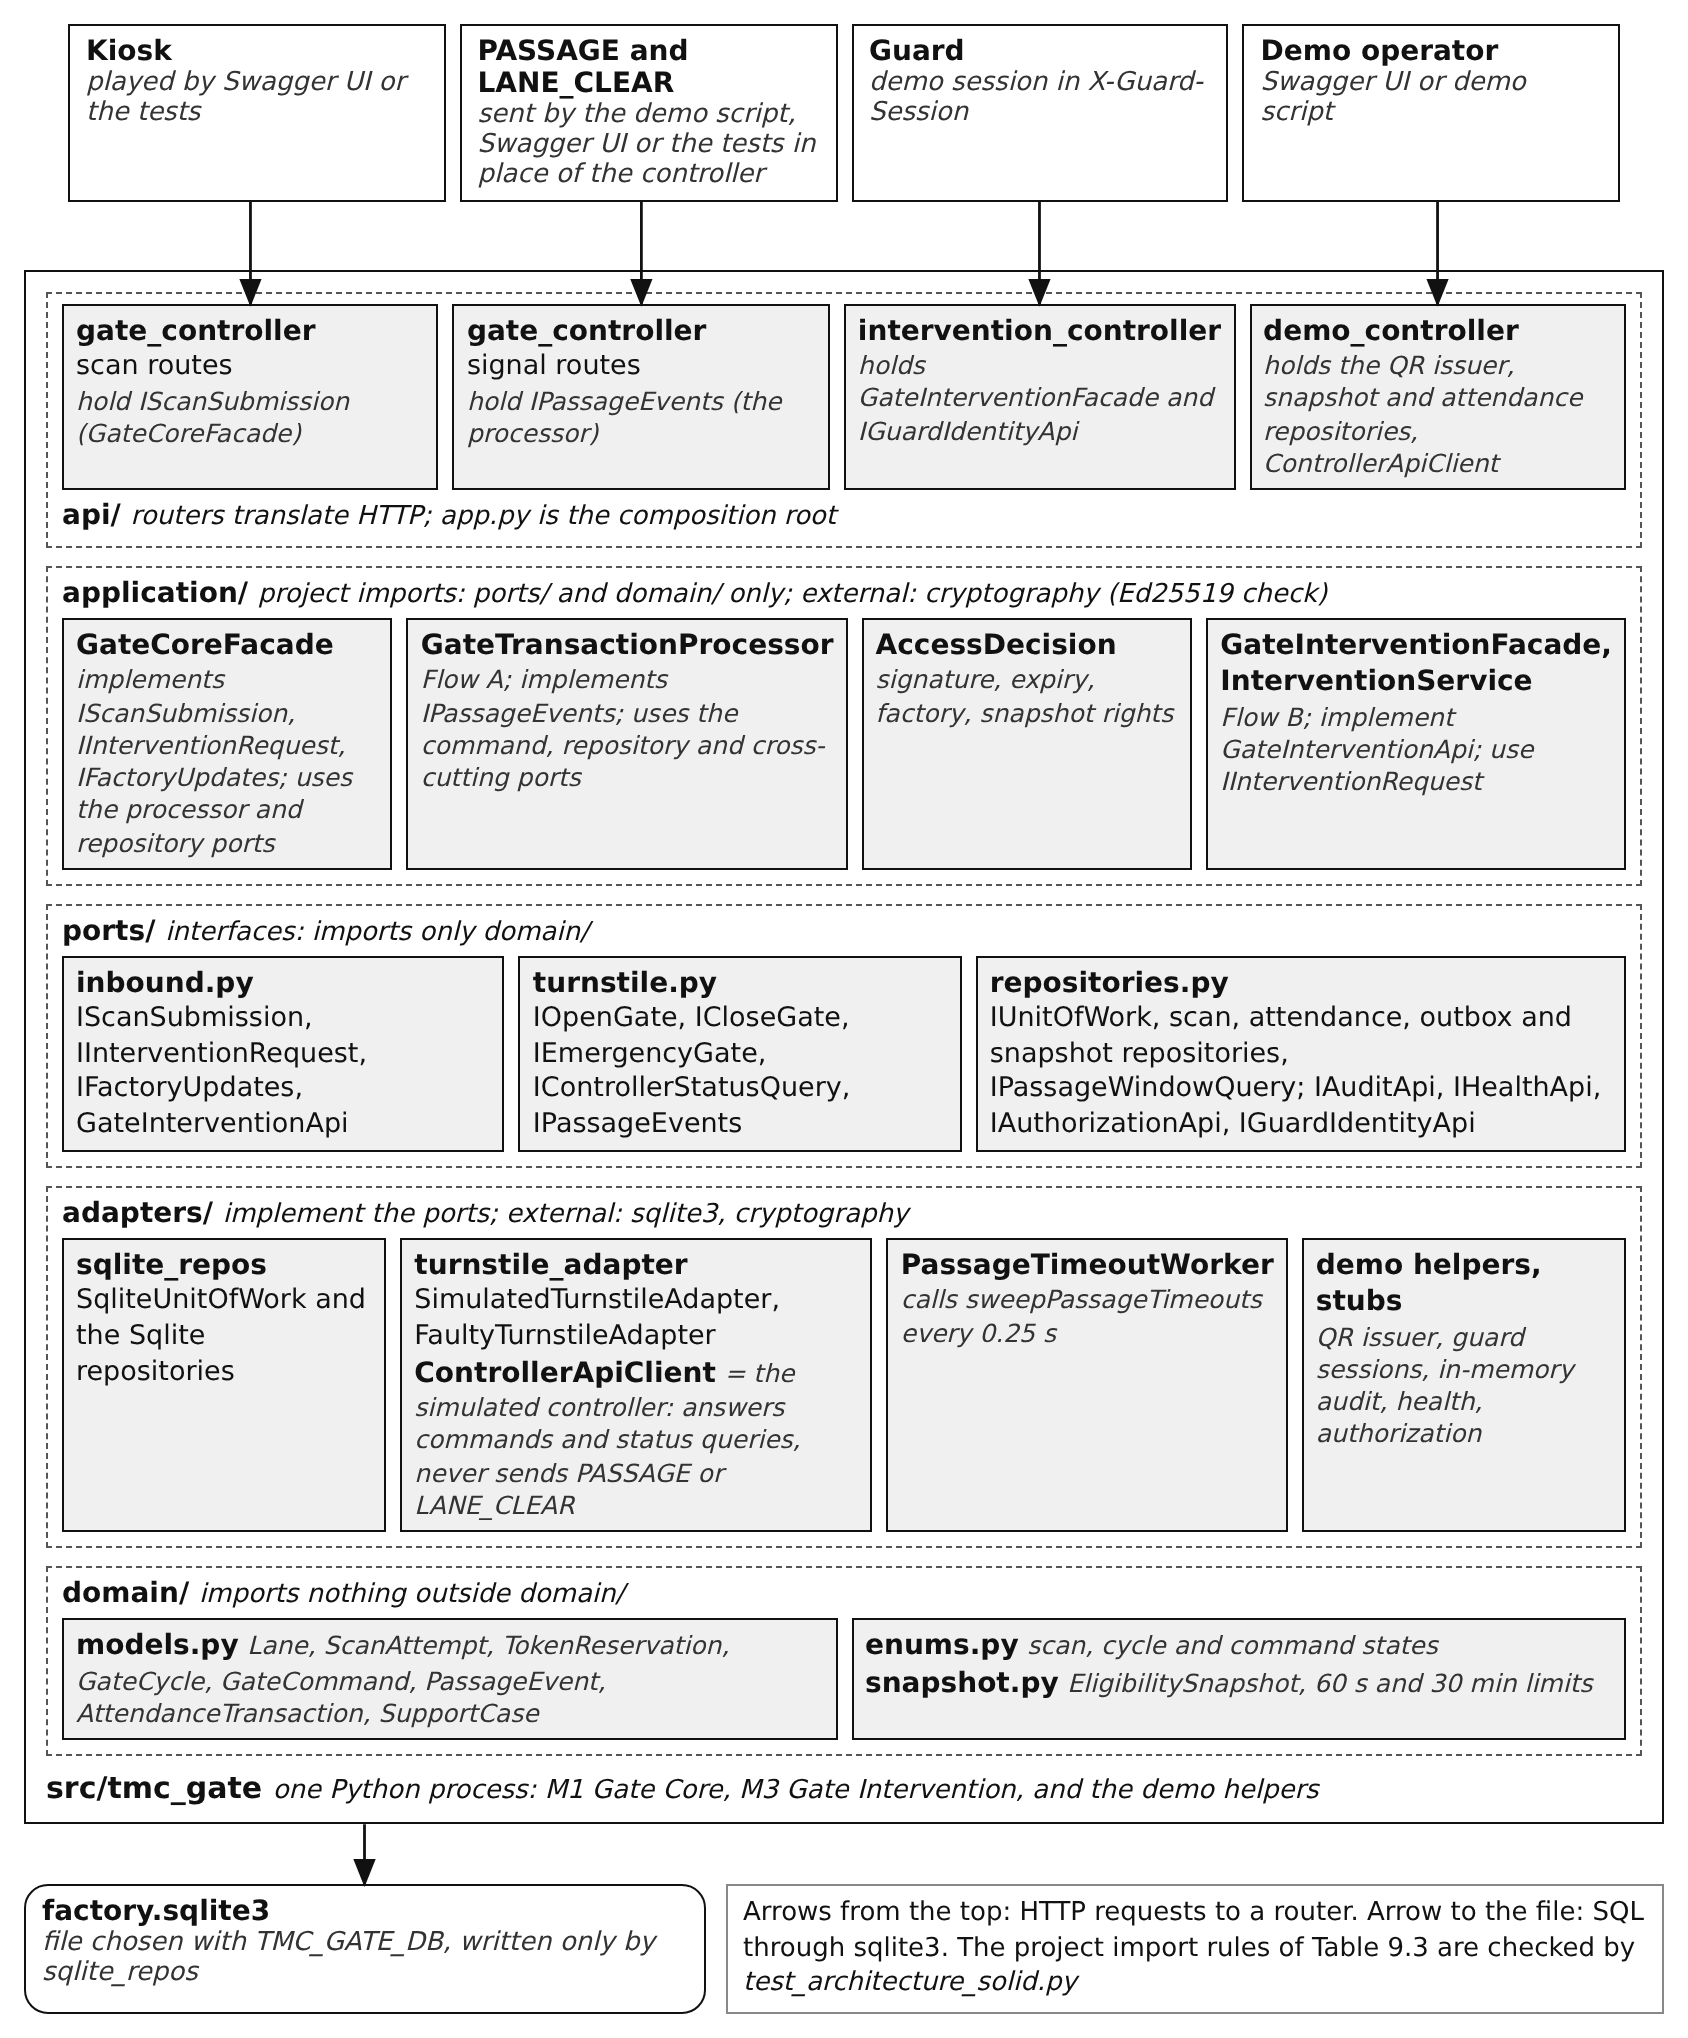
\includegraphics[width=0.98\linewidth]{diagram/implementation/figure-9-1-prototype-structure.png}

\vspace{6pt}
\textbf{Figure 9.1. Internal Structure of the Task 2 Prototype}
\phantomsection\addcontentsline{lof}{figure}{\protect\numberline{9.1}Internal Structure of the Task 2 Prototype}
\end{minipage}

\vspace{10pt}

\Needspace{9\baselineskip}
\subsubsection*{9.3.2. From the Design to the Code}

\phantomsection
\addcontentsline{toc}{subsubsection}{9.3.2. From the Design to the Code}

We tried to keep the names of Chapter 4 in the code, so a reader can take a component from a table or a figure and find it in a file. Table 9.4 lists the main pairs.

\begin{longtable}{|>{\raggedright\arraybackslash}p{150.5pt}|>{\raggedright\arraybackslash}p{260.5pt}|}
\hline
\multicolumn{1}{|>{\columncolor{tableheader}\centering\arraybackslash}p{150.5pt}|}{\textbf{Design element}} & \multicolumn{1}{>{\columncolor{tableheader}\centering\arraybackslash}p{260.5pt}|}{\textbf{Where it is in the code}} \\
\hline
\endhead
\multicolumn{2}{c}{\rule{0pt}{20pt}\normalsize\textbf{Table 9.4. Mapping from the Design to the Code}} \\
\endlastfoot
GateCoreController (Table 4.7) & \code{api/gate_controller.py} for the HTTP routes and GateCoreFacade in \code{application/facade.py}, which implements GateCoreApi \\
\hline
ControllerSignalHandler (Table 4.7) & The two signal routes in \code{api/gate_controller.py}; they call onPassage and onLaneClear of GateTransactionProcessor through IPassageEvents \\
\hline
GateTransactionProcessor (Table 4.7) & \code{application/processor.py} \\
\hline
AccessDecision, EligibilitySnapshot (Table 4.7) & \code{application/access_decision.py}, \code{domain/snapshot.py} \\
\hline
ScanRepo, AttendanceRepo, OutboxRepo (Table 4.7) & Ports in \code{ports/repositories.py}; SqliteScanRepository, SqliteAttendanceRepository, SqliteOutboxRepository, and SqliteUnitOfWork in \code{adapters/sqlite_repos.py} \\
\hline
GateInterventionController, Facade, InterventionService (Table 4.9) & \code{api/intervention_controller.py}; InterventionService and GateInterventionFacade in \code{application/intervention.py} \\
\hline
TurnstileAdapter, ControllerApiClient (Table 4.8) & SimulatedTurnstileAdapter, FaultyTurnstileAdapter, and ControllerApiClient in \code{adapters/turnstile_adapter.py} \\
\hline
GateCoreApi and the turnstile ports (Table 4.20) & \code{ports/inbound.py} (IScanSubmission, IInterventionRequest, IFactoryUpdates) and \code{ports/turnstile.py} (IOpenGate, ICloseGate, IEmergencyGate, IPassageEvents, IControllerStatusQuery) \\
\hline
Entities and states (Figure 4.20, Tables 4.23a--b) & \code{domain/models.py} and \code{domain/enums.py} \\
\hline
15-second passage window (Table 4.23b) & PassageTimeoutWorker in \code{adapters/passage_timeout_worker.py}, which calls GateTransactionProcessor.sweepPassageTimeouts \\*
\hline\noalign{\nobreak}
QR credential issuance in M4 (ADR-11) & QrCredentialIssuance in \code{adapters/demo_qr_issuer.py}, a demo stand-in for the central issuer \\
\hline
\end{longtable}
\phantomsection\addcontentsline{lot}{table}{\protect\numberline{9.4}Mapping from the Design to the Code}

Two names do not appear as classes. GateCoreController became a thin FastAPI router plus GateCoreFacade, because the router should only translate HTTP and the facade is what other modules see. ControllerSignalHandler became two routes that call the processor directly, since a separate class would only forward the call. StationClient, the kiosk application of the target design, is not built at all; Swagger UI and the tests play its role. The class diagrams in Figures 4.18 to 4.20 were drawn from this code, so they use the same names as Table 9.4.

\Needspace{9\baselineskip}
\subsubsection*{9.3.3. Factory Database}

\phantomsection
\addcontentsline{toc}{subsubsection}{9.3.3. Factory Database}

Figure 9.2 shows the tables that the SQLite adapters create in the factory database file, which is chosen with the \texttt{TMC\_GATE\_DB} variable. Each gate record has its own table. Next to them are the outbox, the marks used to drop repeated incoming events, the local audit evidence, and the last applied eligibility snapshot. EmployeeRight does not get a table of its own; its values are kept inside \code{eligibility_snapshots.snapshot_json}.

\noindent\begin{minipage}{\linewidth}
\centering
\IfFileExists{diagram/data/figure-9-2-data-view.png}{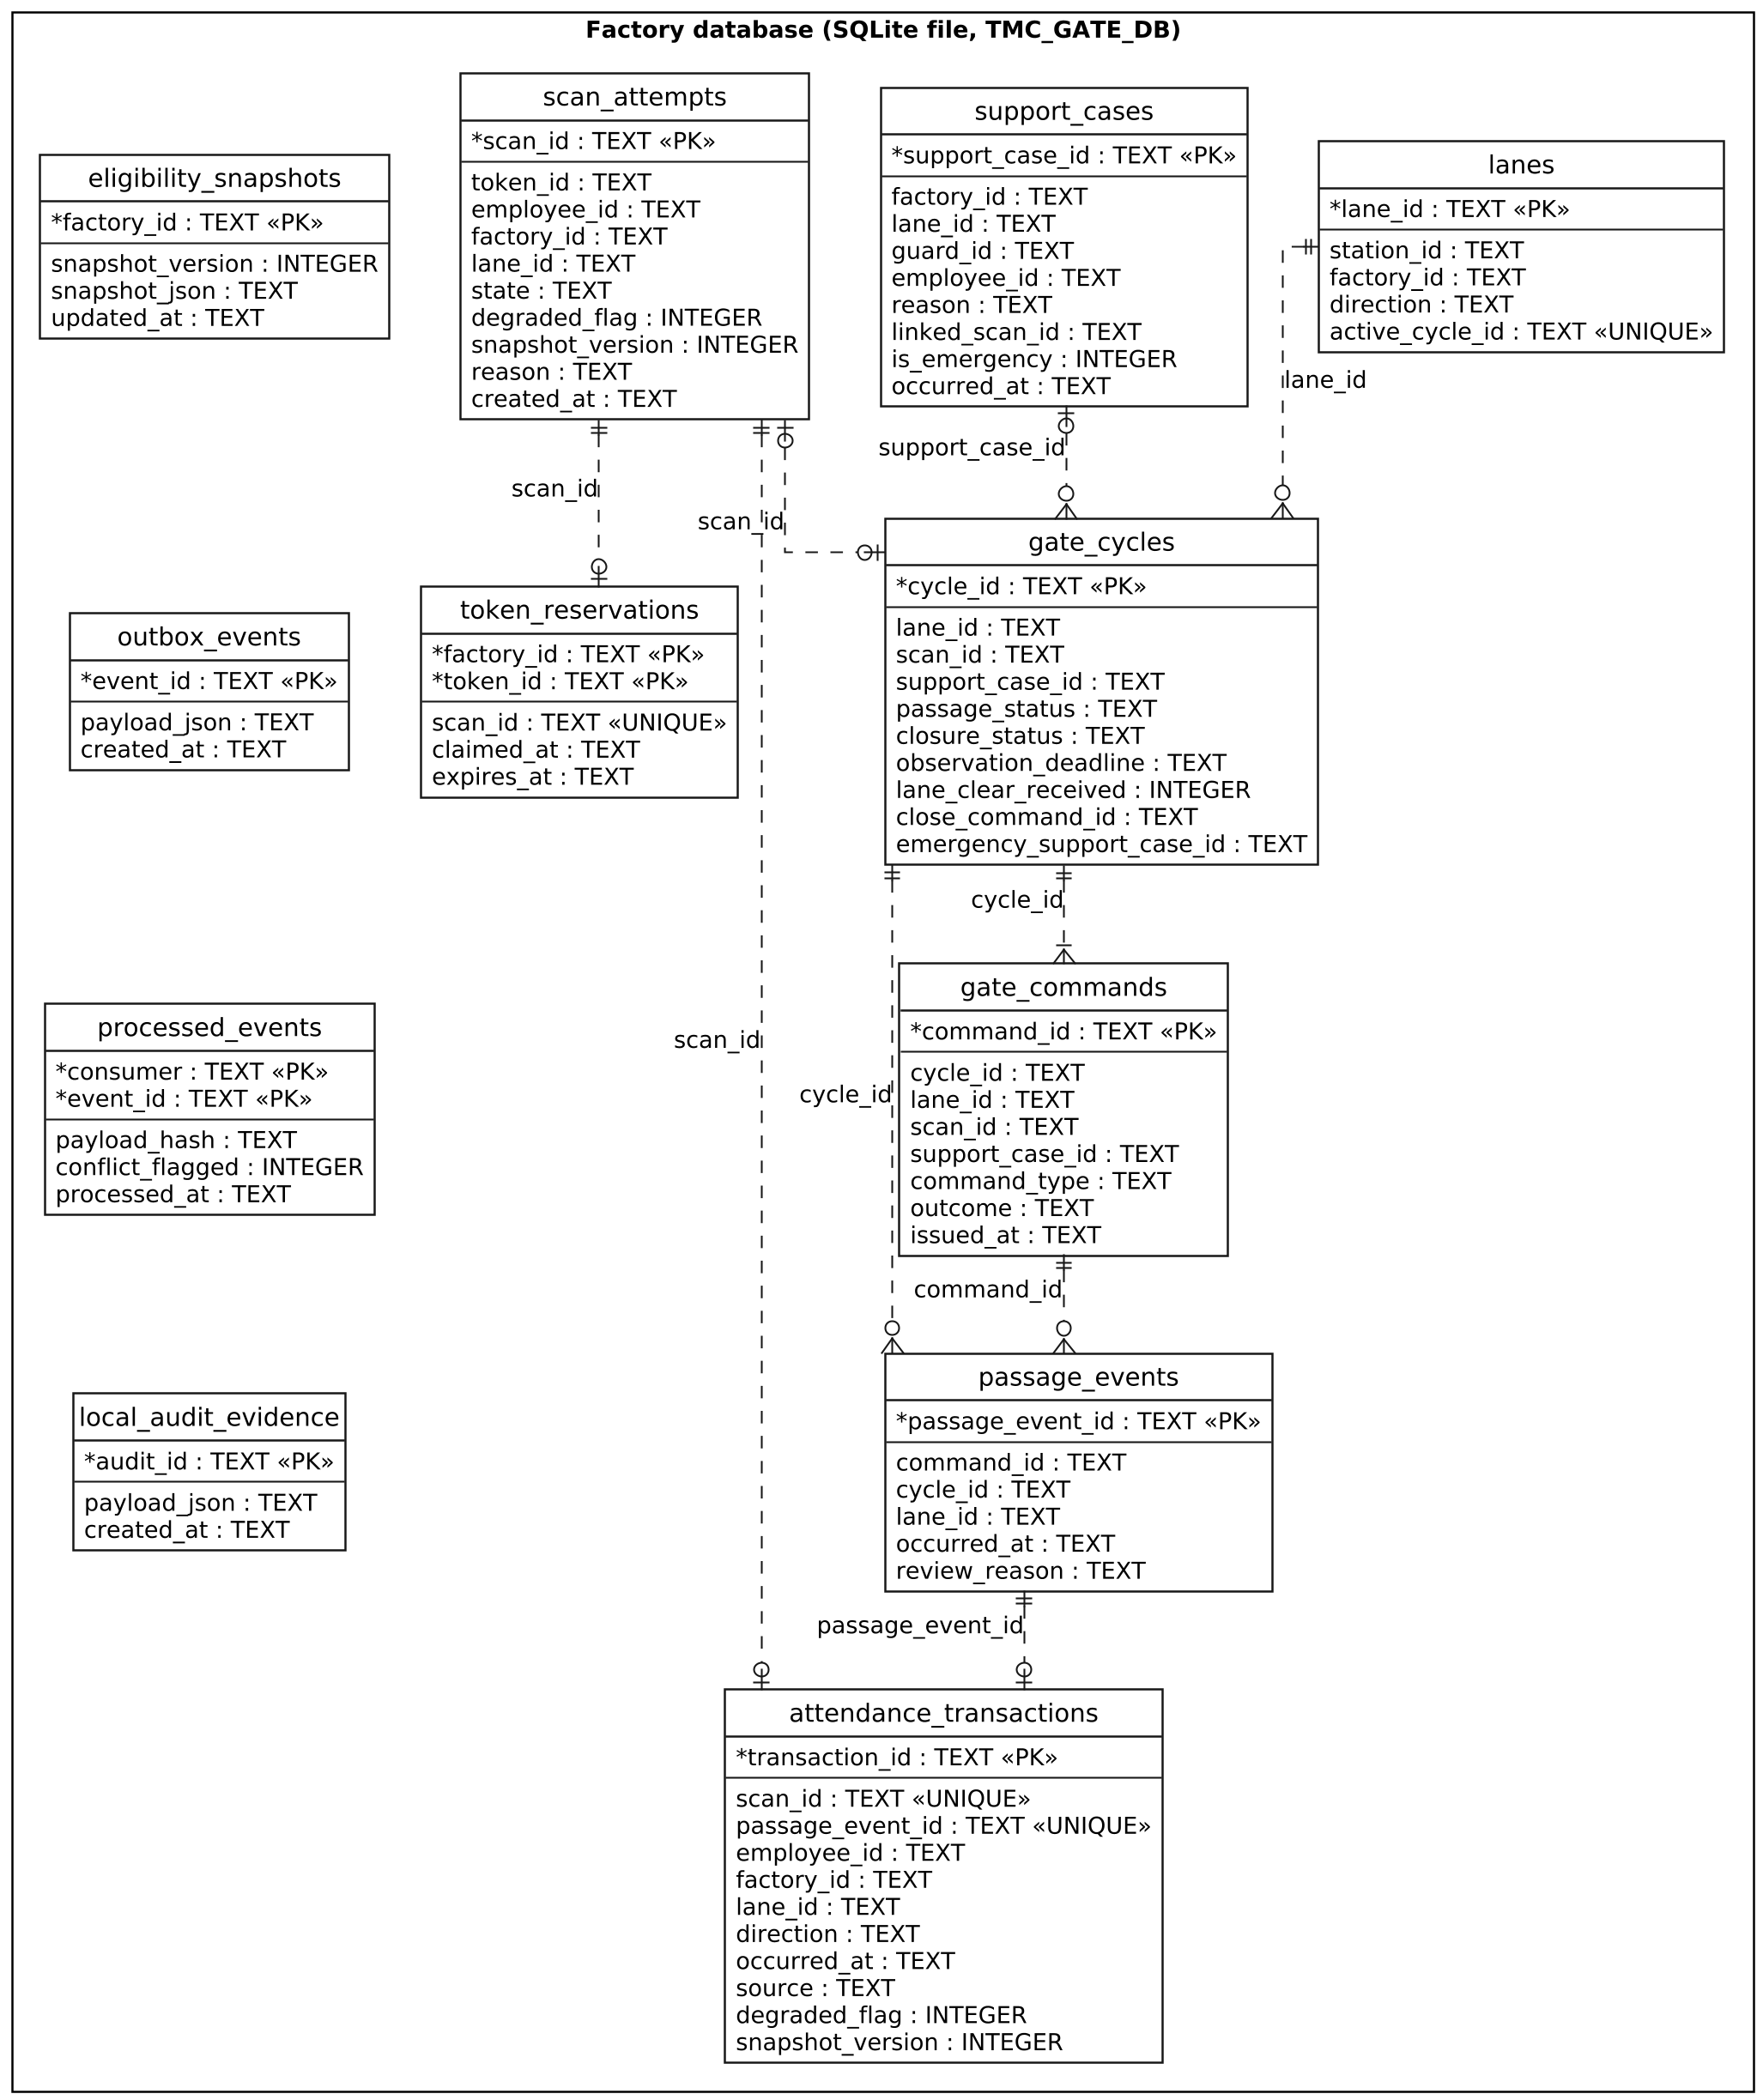
\includegraphics[width=\linewidth,height=430pt,keepaspectratio]{diagram/data/figure-9-2-data-view.png}}{\fbox{\parbox{300pt}{\centering\vspace{20pt}Figure being redrawn\vspace{20pt}}}}

\vspace{6pt}
\textbf{Figure 9.2. Data View of the Factory Database in the Prototype}
\phantomsection\addcontentsline{lof}{figure}{\protect\numberline{9.2}Data View of the Factory Database in the Prototype}
\end{minipage}

\vspace{10pt}

The schema has no foreign key constraints, so the dashed lines in Figure 9.2 are references kept by the code, not by SQLite. The rules that matter for duplicates are enforced by keys instead:

\begin{itemize}[leftmargin=36pt, itemsep=2pt, topsep=4pt, parsep=2pt]
  \item the primary key (factory\_id, token\_id) of \code{token_reservations} makes the claim of a QR token single-use, even for two connections at the same time;
  \item \code{lanes.active_cycle_id} holds at most one active cycle for each lane;
  \item \code{attendance_transactions} has unique scan\_id and passage\_event\_id, so one scan and one PASSAGE give at most one attendance record;
  \item the primary key of \code{passage_events} and of \code{processed_events} (consumer, event\_id) turn a repeated signal or event into a duplicate instead of a second row.
\end{itemize}

A file database runs in write-ahead logging mode, and the unit of work wraps each step of a flow in one transaction.

\Needspace{9\baselineskip}
\subsubsection*{9.3.4. HTTP Endpoints}

\phantomsection
\addcontentsline{toc}{subsubsection}{9.3.4. HTTP Endpoints}

Figure 9.3 is a screenshot of the Swagger page of the running prototype. The endpoints are grouped by who calls them. The kiosk uses the two scan endpoints, which only reach IScanSubmission. The two signal endpoints take PASSAGE and LANE\_CLEAR and reach IPassageEvents; in the prototype they are called by the demo script, Swagger UI, or the tests in place of a real controller. Guards use the three intervention endpoints and must send an \texttt{X-Guard-Session} header, because the guard is taken from the session and not from the request body. The four demo endpoints issue QR codes, change the age of the access data, choose how the simulated controller answers, and list the stored attendance. They are only mounted when \code{demo_mode} is on.

\noindent\begin{minipage}{\linewidth}
\centering
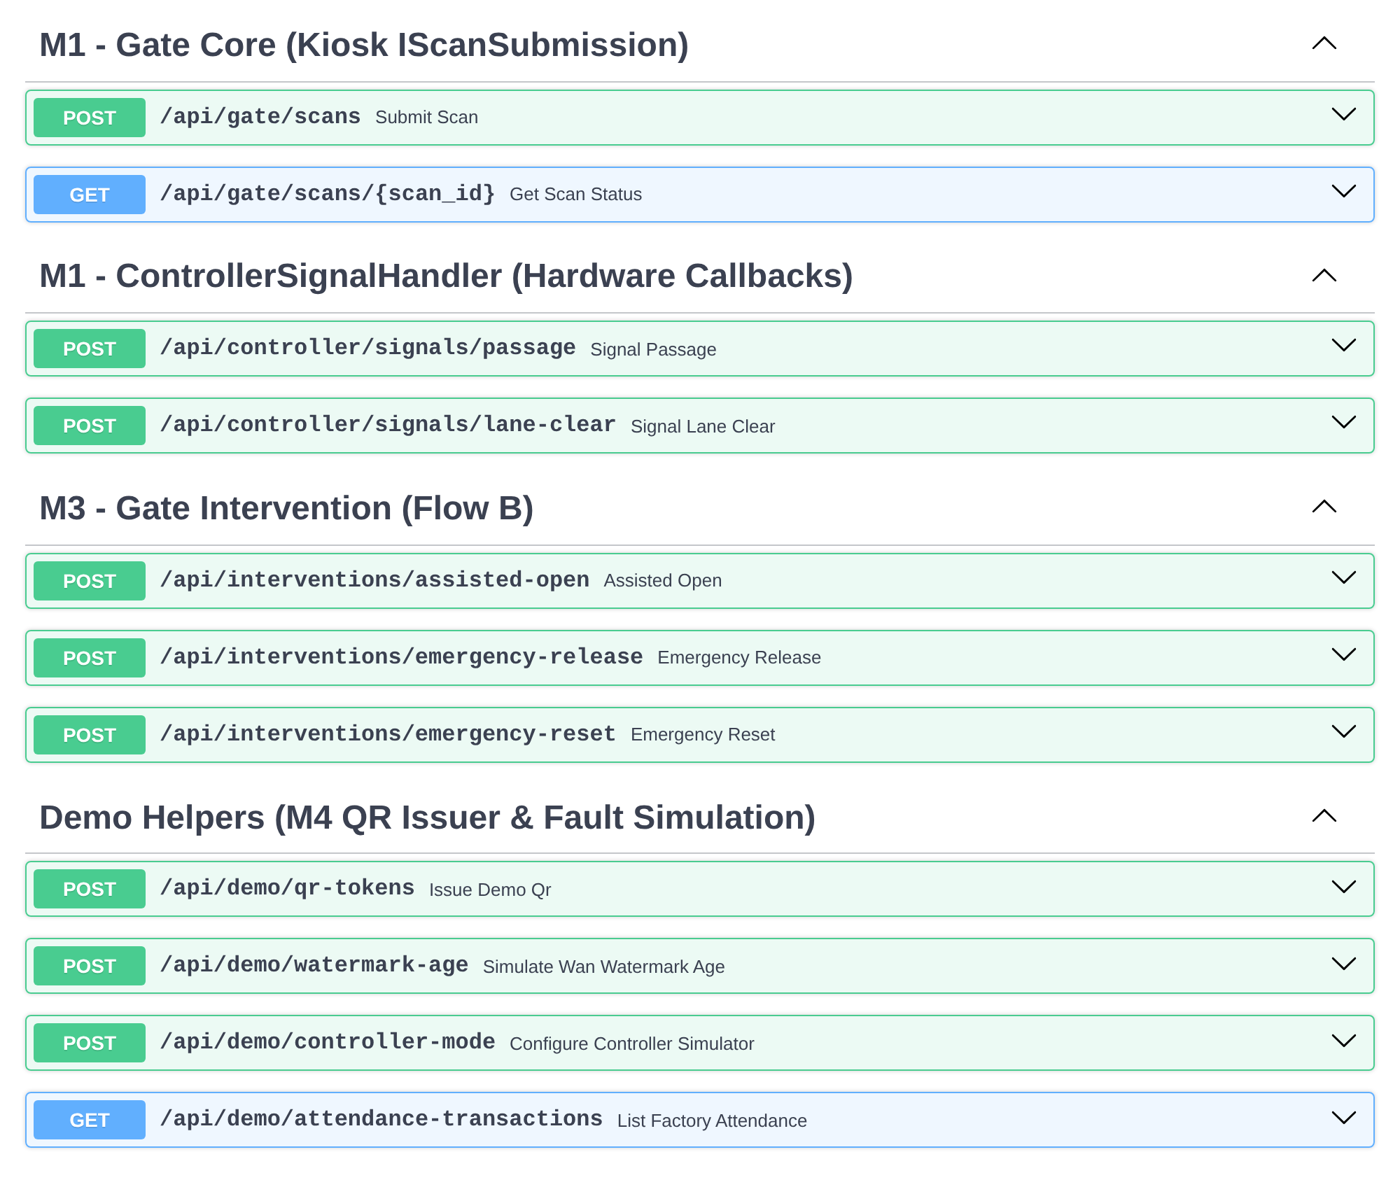
\includegraphics[width=0.82\linewidth]{figure/figure-9-3-swagger-endpoints.png}

\vspace{6pt}
\textbf{Figure 9.3. Endpoints of the Prototype in Swagger UI}
\phantomsection\addcontentsline{lof}{figure}{\protect\numberline{9.3}Endpoints of the Prototype in Swagger UI}
\end{minipage}

\vspace{10pt}

Table 9.5 lists the same endpoints with what each router is given in \code{app.py}. The kiosk and signal routes are typed with a port, so the dependency they declare is narrow. This is not an access control by itself: in Python, \code{app.py} still passes the whole GateCoreFacade object to the kiosk router. What keeps a kiosk from starting an intervention is that no kiosk endpoint calls such an operation, and that the guard endpoints check the guard session on the server. The guard routes get GateInterventionFacade and, for that session check, IGuardIdentityApi. The demo routes are wired directly to demo helpers, which is acceptable only because they are not mounted outside demo mode.

\noindent\begin{minipage}{\linewidth}
\centering
\begin{tabular}{|>{\raggedright\arraybackslash}p{167pt}|>{\raggedright\arraybackslash}p{56pt}|>{\raggedright\arraybackslash}p{88pt}|>{\raggedright\arraybackslash}p{84pt}|}
\hline
\multicolumn{1}{|>{\columncolor{tableheader}\centering\arraybackslash}p{167pt}|}{\textbf{Method and path}} & \multicolumn{1}{>{\columncolor{tableheader}\centering\arraybackslash}p{56pt}|}{\textbf{Caller}} & \multicolumn{1}{>{\columncolor{tableheader}\centering\arraybackslash}p{88pt}|}{\textbf{Router is given}} & \multicolumn{1}{>{\columncolor{tableheader}\centering\arraybackslash}p{84pt}|}{\textbf{Result}} \\
\hline
\code{POST /api/gate/scans} & Kiosk & IScanSubmission & Scan state, reason, commandId (A1--A7) \\
\hline
\code{GET /api/gate/scans/{scanId}} & Kiosk & IScanSubmission & Stored state after a lost response; 404 if unknown \\
\hline
\code{POST /api/controller/signals/passage} & Controller (played) & IPassageEvents & PASSAGE handled (A8) \\
\hline
\code{POST /api/controller/signals/lane-clear} & Controller (played) & IPassageEvents & LANE\_CLEAR handled, closeGate (A9) \\
\hline
\code{POST /api/interventions/assisted-open} & Guard & GateIntervention\-Facade & Support case and assisted openGate; 401 without a session \\
\hline
\code{POST /api/interventions/emergency-release} & Guard & GateIntervention\-Facade & EMERGENCY\_\allowbreak HOLD on the lane \\
\hline
\code{POST /api/interventions/emergency-reset} & Guard & GateIntervention\-Facade & Reset of the emergency that holds the lane \\
\hline
\code{POST /api/demo/qr-tokens} & Demo only & QR issuer helper & Signed 60-second token \\
\hline
\code{POST /api/demo/watermark-age} & Demo only & Snapshot storage & Operating mode after ageing the watermark \\
\hline
\code{POST /api/demo/controller-mode} & Demo only & ControllerApi\-Client & How the next commands and queries are answered \\
\hline
\code{GET /api/demo/attendance-transactions} & Demo only & Attendance storage & Stored attendance records \\
\hline
\end{tabular}

\vspace{6pt}
\textbf{Table 9.5. HTTP Endpoints of the Prototype}
\end{minipage}

\vspace{10pt}
\phantomsection\addcontentsline{lot}{table}{\protect\numberline{9.5}HTTP Endpoints of the Prototype}

\Needspace{9\baselineskip}
\subsection*{9.4. SOLID in the Code}

\phantomsection
\addcontentsline{toc}{subsection}{9.4. SOLID in the Code}

Section 7.1 explains how SOLID shaped the modules on paper. Here we look at where each principle shows up in the code and, where one exists, which test checks it.

The single responsibility principle is about actors: a module should answer to one group of people who ask for the same kind of change. ``One reason to change'' says the same thing, as long as the reason is traced back to who asks for it. In our code, the gate rules are asked for by the people who run the factory gates and security, while shift and payroll rules come from HR. Because of I-06, a change in the shift or attendance rules of HR does not reach the gate decision: AccessDecision (\code{application/access_decision.py}) only checks the token against the snapshot and returns a DecisionResult, and it has no shift input and no turnstile port. The rules about how fresh the access data must be live in EligibilitySnapshot (\code{domain/snapshot.py}), and InterventionService only checks what a guard is allowed to do and leaves the gate commands to Gate Core.

GateTransactionProcessor is the largest class, and its size alone does not show that SRP holds or fails. Its responsibility is to coordinate the life cycle of one gate transaction: accept the scan, reserve the lane, open, handle PASSAGE and LANE\_CLEAR, close, and handle the emergency commands on the same lane. The eligibility check, the storage, and the controller protocol have been moved out to AccessDecision, the repositories, and the adapters, so a change in one of them does not edit the processor. GateCoreFacade is a thin entry point that turns the inbound ports into processor calls; its name is not evidence of SRP either. Because of the split, \code{test_pkg1_snapshot.py} can test the snapshot rules alone, and \code{test_pkg2_access_decision.py} can call AccessDecision.evaluate twice on the same data and check that it gives the same answer without changing anything.

For the open/closed principle, the place that changes is the controller. The ports in \code{ports/turnstile.py} belong to Gate Core, and the adapters depend on them, not the other way round. A new turnstile model would be a new class in \code{adapters/} that implements ITurnstileControl, and \code{api/app.py} decides which adapter is passed in. This is close to the Strategy idea from the lecture: the processor keeps its rules and only the object behind the port is swapped. \code{test_pkg5_adapter_with_processor.py} runs the same GateTransactionProcessor with both adapter classes we have, and the processor did not need any change for the second one.

The Liskov substitution principle matters most for the meaning of a controller result. The port file \code{ports/turnstile.py} fixes the set of results that each command may return. A receipt or a timeout must come back as UNDETERMINED, not as OPEN\_CONFIRMED or CONTROLLER\_ERROR. One contract test file, \code{test_pkg5_turnstile_contract.py}, runs the same checks against SimulatedTurnstileAdapter and FaultyTurnstileAdapter, and both pass. We also wrote a third adapter that reports a receipt as OPEN\_CONFIRMED. It fails the same contract, and this test is marked as an expected failure on purpose.

Interface segregation is judged from the consumer's side. It shows in how GateCoreApi is split into IScanSubmission, IInterventionRequest, and IFactoryUpdates (\code{ports/inbound.py}). The kiosk router only receives IScanSubmission, InterventionService only receives IInterventionRequest, and the controller routes only receive IPassageEvents. On the other side, the processor depends on IOpenGate, ICloseGate, and IEmergencyGate one by one, even though one adapter class implements all three as ITurnstileControl. \code{test_interface_segregation_principle_contracts} checks that the kiosk interface has no intervention or sync operation and that IPassageEvents has only onPassage and onLaneClear. The split is not complete everywhere: IScanRepository still has 14 operations, all used by the processor, while GateCoreFacade only uses get\_scan and save\_scan. Section 8.2 discusses this limitation.

Dependency inversion is what made the group work possible. GateTransactionProcessor receives all its ports and its IUnitOfWork through the constructor, and the application layer does not import \texttt{sqlite3}, \texttt{fastapi}, \code{adapters/}, or \code{api/}. \code{api/app.py} is the composition root: it creates the main dependencies (the SQLite repositories and unit of work, the turnstile adapter, the processor, the facades, and the timeout worker) and connects them. In \code{test_architecture_solid.py}, three import tests check the domain, ports, and application layers one by one, and a fourth test checks the ISP splits. These tests check the direction of dependencies and the shape of the ports; they do not prove all five principles, and SRP and OCP in particular are design judgements supported by the examples above. We wrote and merged the ports before anything else, so six people could work in parallel against fakes. Packages 1, 3, and 6 were finished and tested before the SQLite repositories or the turnstile adapter existed.

Only one port was added after that point. While checking the code before submission we found that a cycle with no PASSAGE could stay OPENED, because nothing triggered the 15-second timeout once LANE\_CLEAR had already released the lane. The processor needed a way to find such cycles by their own state, so we added the small read port IPassageWindowQuery (\code{list_cycles_awaiting_passage}, \code{get_cycle_by_scan}) instead of putting two more methods on IScanRepository. SqliteScanRepository implements it, and PassageTimeoutWorker uses it through the processor (Section 9.5, step A8).

\Needspace{9\baselineskip}
\subsection*{9.5. Following One Scan Through the Code}

\phantomsection
\addcontentsline{toc}{subsection}{9.5. Following One Scan Through the Code}

The tables above show what exists, but not in which order things happen. In this section we follow one QR scan from the kiosk request to the closed gate. Each step carries the label of the matching step in the design sequence of Figure 4.16 and Section 4.2.2, so the two descriptions can be read side by side. The classes are the ones in Figures 4.18 and 4.19, and Figure 9.4 draws the same steps as two sequence diagrams with the names used in the code. Part (a) is the kiosk request, A1 to A7. Part (b) shows A8 and A9, which arrive as their own HTTP requests. Both parts show one successful run as an example. The order in which they are drawn is not an order the code guarantees: the PASSAGE request can be handled before the kiosk has received its A7 response, and LANE\_CLEAR does not wait for PASSAGE.

\noindent\begin{minipage}{\linewidth}
\centering
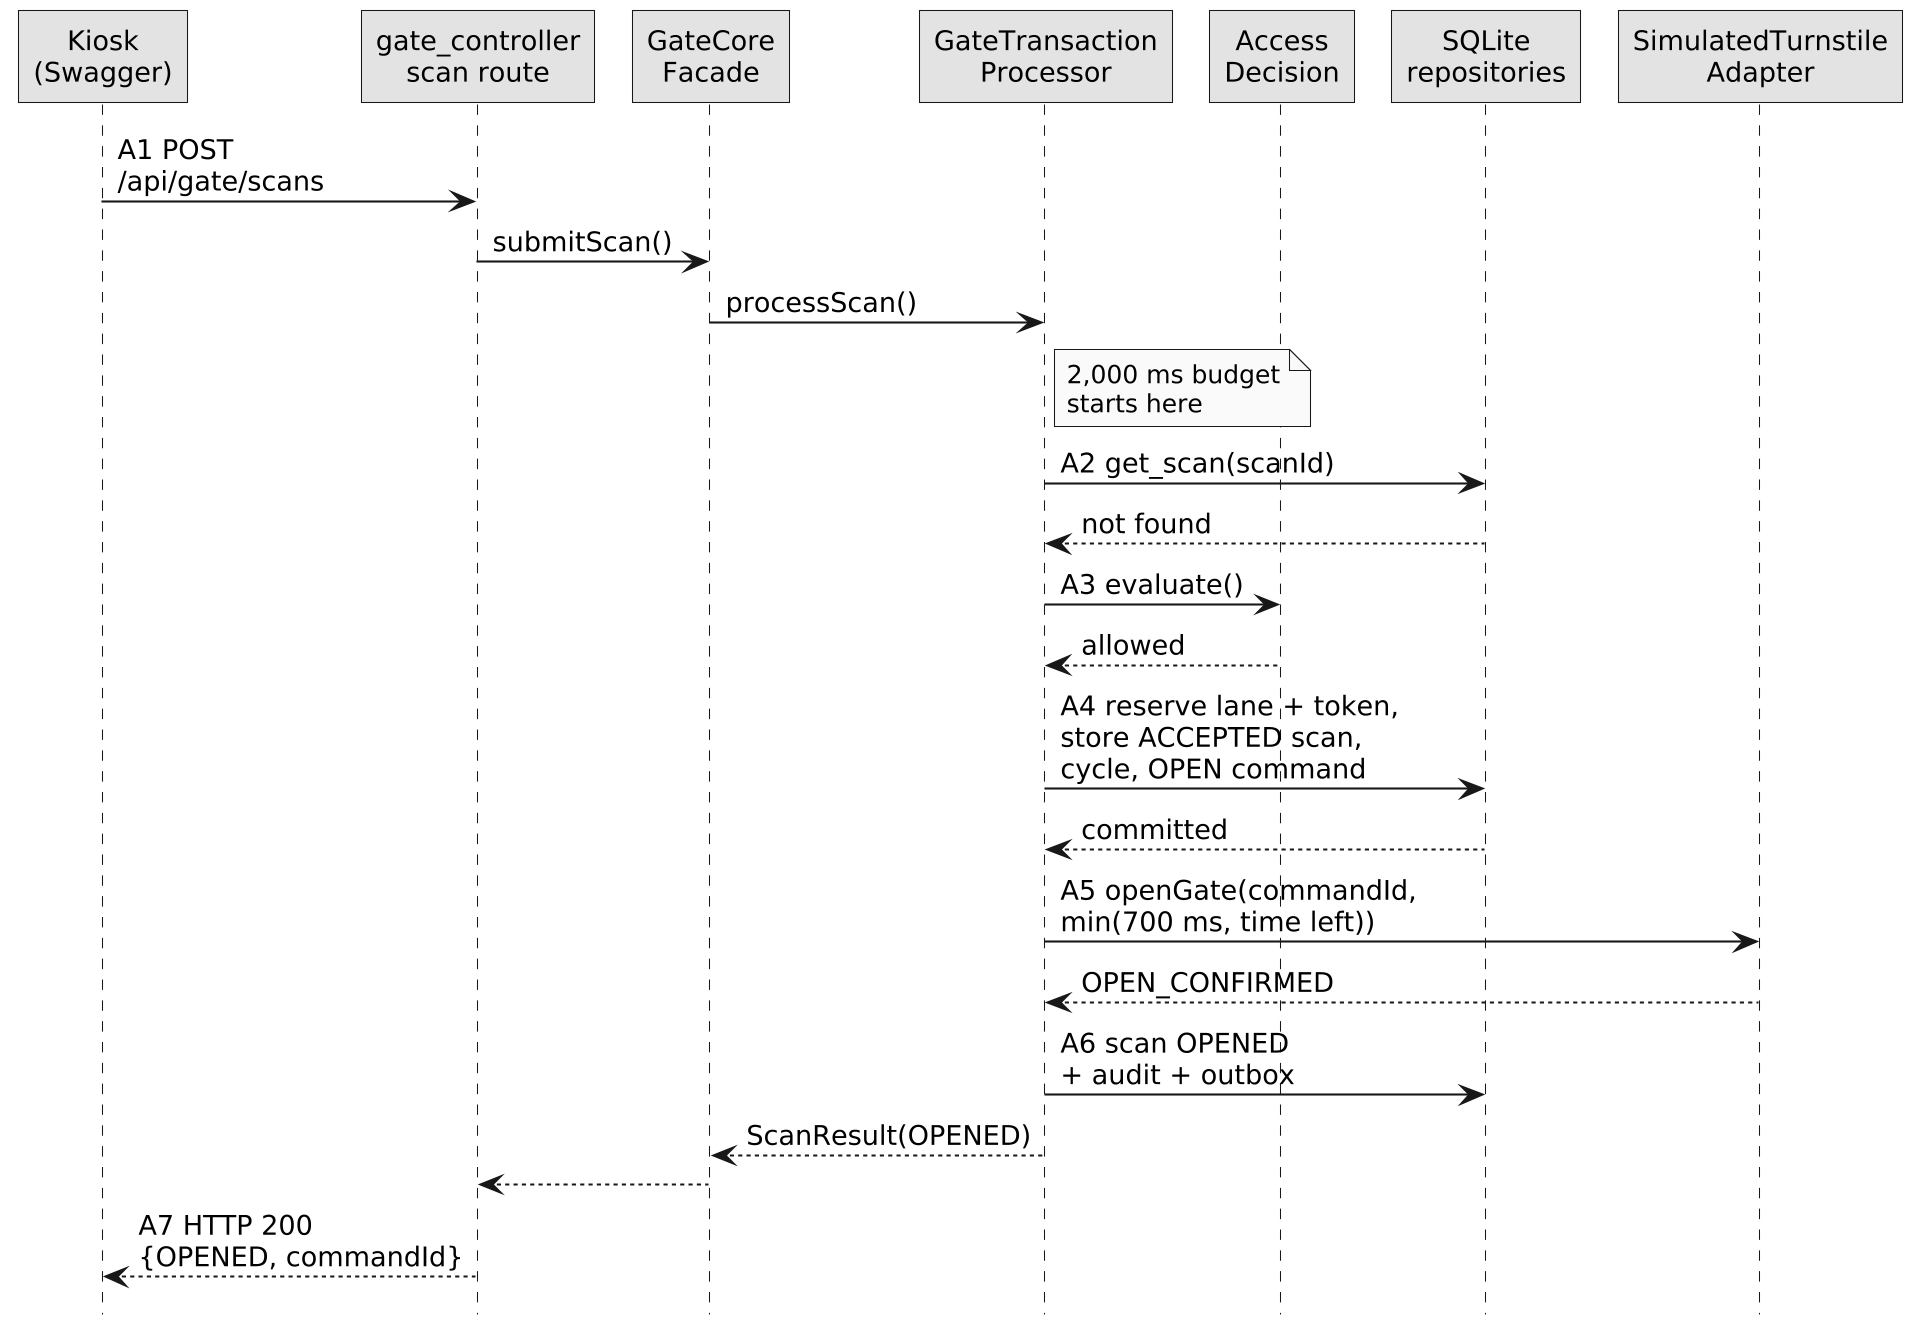
\includegraphics[width=0.94\linewidth]{diagram/implementation/figure-9-4a-scan-request.png}

\vspace{2pt}
{\small (a) Kiosk request, A1--A7}
\end{minipage}

\vspace{8pt}
\noindent\begin{minipage}{\linewidth}
\centering
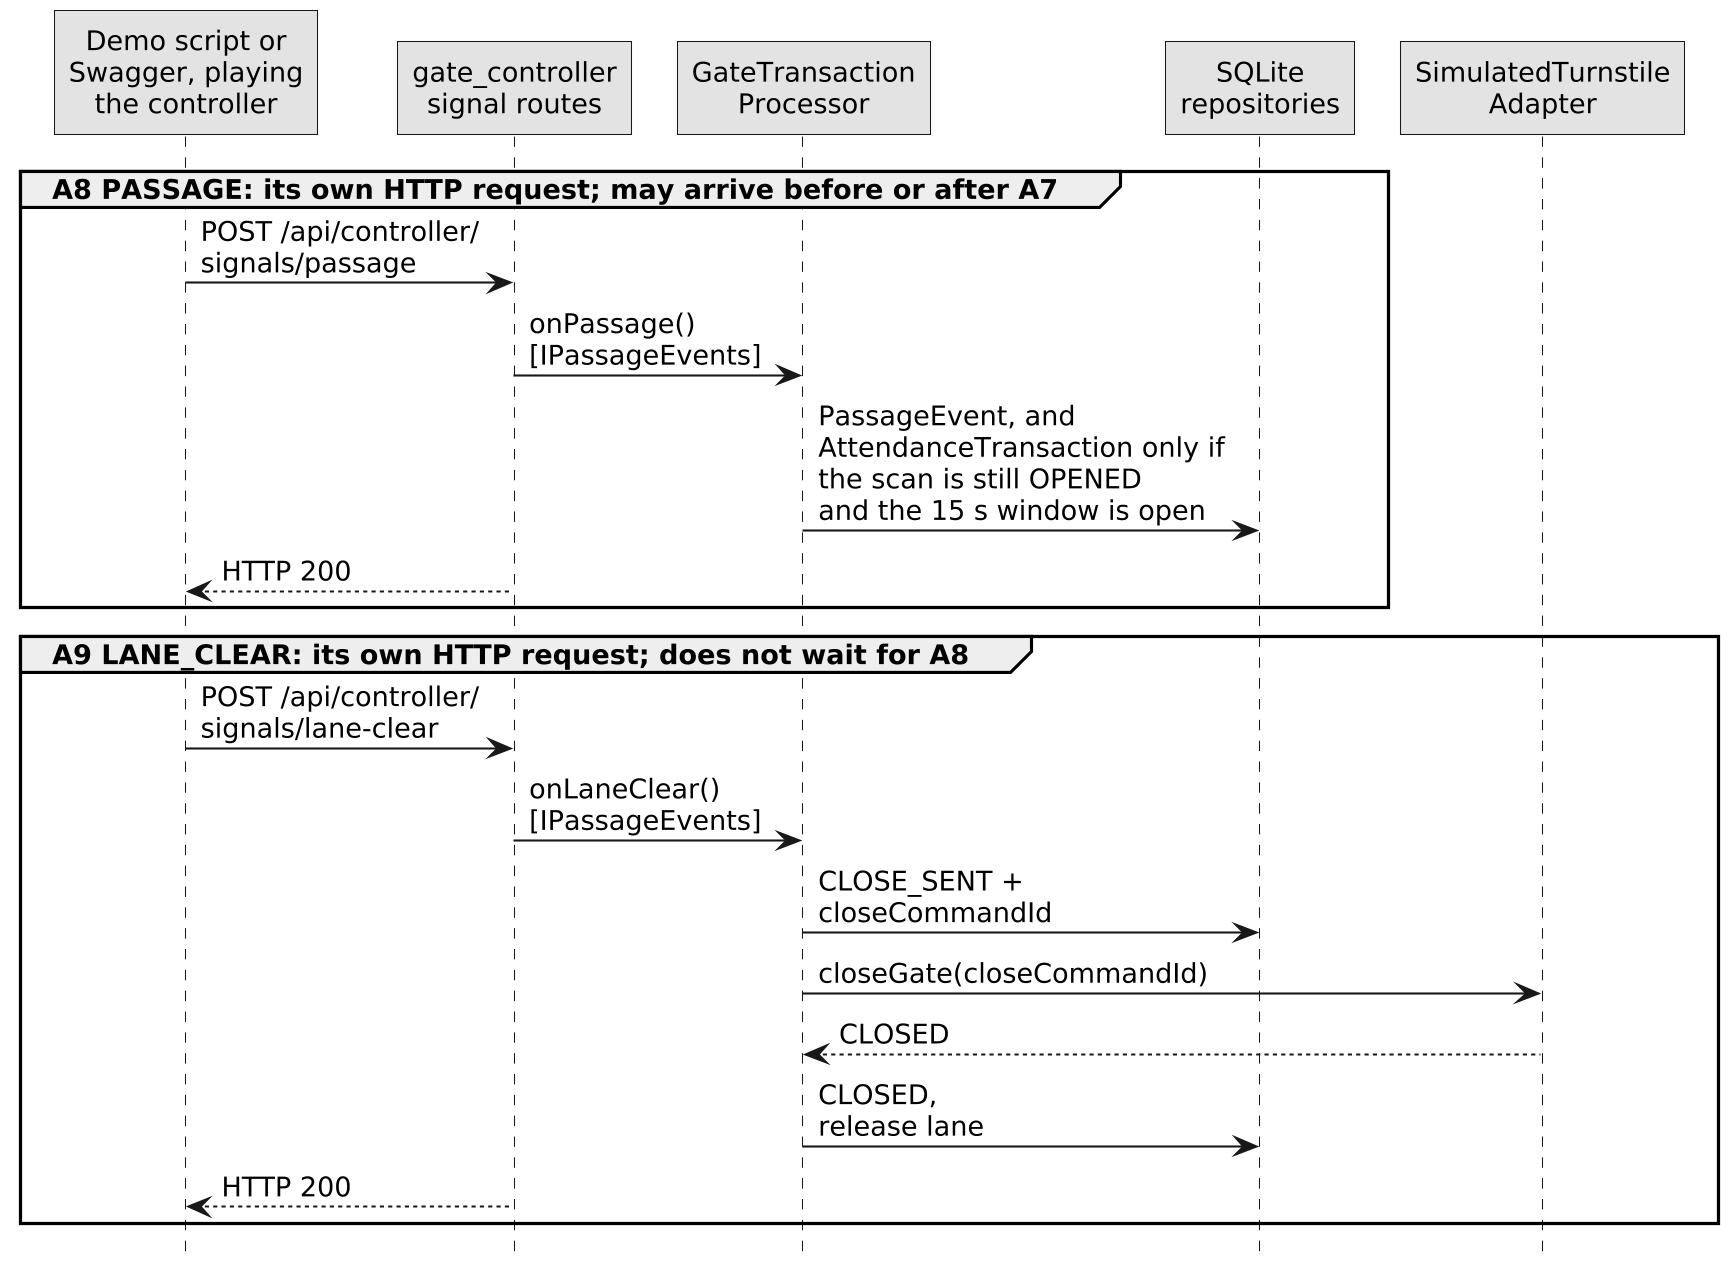
\includegraphics[width=0.86\linewidth]{diagram/implementation/figure-9-4b-controller-signals.png}

\vspace{2pt}
{\small (b) Controller signals, A8 and A9: separate requests, in any order relative to (a) and to each other}

\vspace{6pt}
\textbf{Figure 9.4. Flow A as Implemented: One Scan from the Kiosk Request to the Closed Gate}
\phantomsection\addcontentsline{lof}{figure}{\protect\numberline{9.4}Flow A as Implemented}
\end{minipage}

\vspace{10pt}

\begin{itemize}[leftmargin=36pt, labelwidth=22pt, labelsep=8pt, align=left, itemsep=3pt, topsep=4pt, parsep=2pt]
  \item[\textbf{A1}] The kiosk sends \code{POST /api/gate/scans} with a scanId, the QR text, and the laneId. The route only holds an IScanSubmission, so it calls GateCoreFacade.submitScan, which hands the scan to GateTransactionProcessor.processScan. From here the processor counts down a processing budget, and every later step only gets the time that is left. The HTTP route does not pass a kiosk deadline, so this budget is a full 2,000 ms that starts when processScan begins (Section 9.8).
  \item[\textbf{A2}] The processor first looks the scanId up in storage. If the kiosk is retrying a request whose answer was lost, the stored result is returned unchanged and nothing else runs.
  \item[\textbf{A3}] AccessDecision.evaluate reads the current EligibilitySnapshot and checks the operating mode first. If the access data is too old or the clock error is too large, the answer is CANNOT\_PROCESS before the QR code is even read. Otherwise it verifies the Ed25519 signature, the 60-second expiry, and the factory of the token, and then asks the snapshot whether this employee may use this lane. A scan that fails is stored as REJECTED or CANNOT\_PROCESS with an audit record, and the kiosk gets the reason.
  \item[\textbf{A4}] For an allowed scan the processor prepares four records: the ACCEPTED ScanAttempt, a TokenReservation for the tokenId, a new GateCycle for the lane, and the OPEN GateCommand. SqliteScanRepository writes all four in one transaction. If the lane already has an active cycle, nothing is written and the answer is LANE\_BUSY. If the tokenId has been claimed before, for example by a copy of the QR code on another lane, the scan is stored as REJECTED with the reason QR\_TOKEN\_REPLAY\_DETECTED.
  \item[\textbf{A5}] Only after this commit does the processor call openGate, with a timeout of min(700 ms, time left). If no time is left at this point, the command is not sent: the scan ends as CANNOT\_PROCESS and the lane is released, but the token stays claimed.
  \item[\textbf{A6}] The controller result decides the next state. With OPEN\_CONFIRMED the scan becomes OPENED and the 15-second passage window starts; the outbox event and the audit record go into the same transaction. With CONTROLLER\_ERROR the lane is released. An UNDETERMINED result is stored first, and the controller is asked once through IControllerStatusQuery where the adapter supports it. If there is no status query, or the answer is still unclear, the scan becomes PENDING\_RECONCILIATION.
  \item[\textbf{A7}] processScan returns this state to the route, and the kiosk receives it in the HTTP response. This is where the server-side part of the scan ends. NFR-01 itself is measured until the kiosk displays the result (Section 1.7), and the prototype does not measure that. Returning the opening result does not create attendance. Attendance is recorded separately when a valid PASSAGE is processed, independently of when the kiosk receives its response.
  \item[\textbf{A8}] Attendance comes from the passage, not from the opening. When the employee walks through, the controller calls \code{POST /api/controller/signals/passage}. This request reaches onPassage on the processor through IPassageEvents, and it is handled on its own, separately from the kiosk request. In one transaction the processor stores the PassageEvent and, if the scan is still OPENED and the window has not ended, the AttendanceTransaction. A passage that comes too late is still stored, but with the review reason LATE\_PASSAGE and without attendance. If no PASSAGE arrives at all, PassageTimeoutWorker, which wakes up every 0.25 seconds, makes the processor mark the cycle as NO\_PASSAGE and the scan as PENDING\_RECONCILIATION once the 15 seconds are over. The worker does not close the gate.
  \item[\textbf{A9}] Closing waits for LANE\_CLEAR, whether or not a passage was recorded. The signal arrives at \code{/api/controller/signals/lane-clear}, and onLaneClear first stores CLOSE\_SENT and the closeCommandId. Only then does it call closeGate. The lane becomes free again when the result is CLOSED.
\end{itemize}

We also ran these steps by hand on a team member's Windows laptop, against a real \texttt{uvicorn} server in demo mode, with \code{TMC_GATE_DB} pointing to a SQLite file and the simulated controller. The server ran in one PowerShell window and the client in a second one, using the script \code{report/evidence/run_demo.py}. Figure 9.5 is a screenshot of the second window. The script first marks the access data as just confirmed, because the prototype has no Site Sync and the server only treats its data as fresh at start-up; without this step a run started more than 60 seconds after the server would come out DEGRADED. We took a signed QR code for employee EMP-001 from the demo endpoint and used it twice: S-1 on LANE-BD-01 was OPENED (a), and S-2 with the same code on LANE-BD-02 was REJECTED with QR\_TOKEN\_REPLAY\_DETECTED (b). We then played the controller and sent PASSAGE and LANE\_CLEAR twice each for the commandId of S-1 (c). The HTTP answers alone do not show that the repeats were ignored, so in (d) we opened the database file with a separate connection. It holds one attendance record, linked to S-1 and passage event PE-1, one passage event, and exactly one OPEN and one CLOSE command. Table 9.8 in Section 9.7 sums up what each part of the run shows.

\noindent\begin{minipage}{\linewidth}
\centering
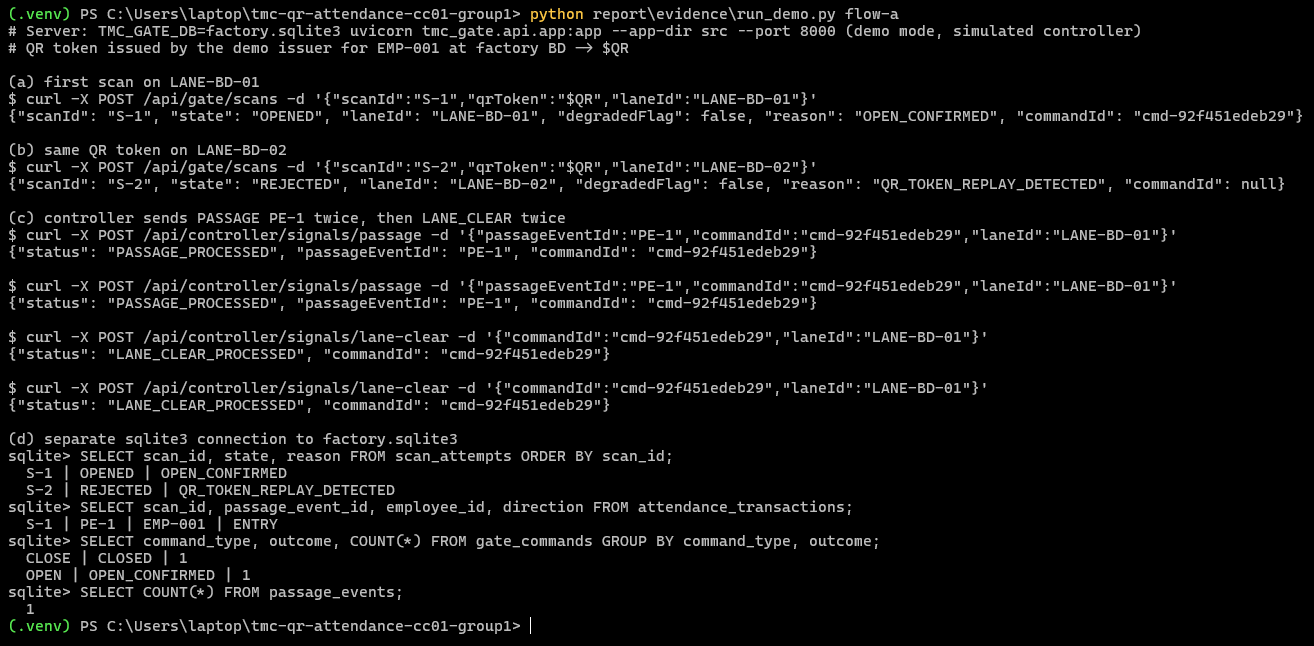
\includegraphics[width=\linewidth]{figure/figure-9-5-flow-a-run.png}

\vspace{6pt}
\textbf{Figure 9.5. Flow A on Uvicorn with a SQLite File: Repeated Signals Give One Attendance Record}
\phantomsection\addcontentsline{lof}{figure}{\protect\numberline{9.5}Flow A on Uvicorn with a SQLite File}
\end{minipage}

\vspace{10pt}

The run in Figure 9.5 only covers the normal path. We ran the same script twice more, each time with a fresh SQLite file, to show what happens when something is not normal. In Figure 9.6 we first aged the access data to 300 seconds: scan S-10 was still OPENED, but with the degraded flag, and the attendance record created from its passage carries the same flag (a). At 1800 seconds the next scan was refused with CANNOT\_PROCESS before any command (b). We then made the access data fresh again and set the simulated controller so that openGate times out and the status query cannot tell the result. Scan S-12 ended as PENDING\_RECONCILIATION, and a new scan on the same lane got LANE\_BUSY because the lane stays held (c). The database shows a single OPEN command for S-12 with the outcome UNDETERMINED (d).

\noindent\begin{minipage}{\linewidth}
\centering
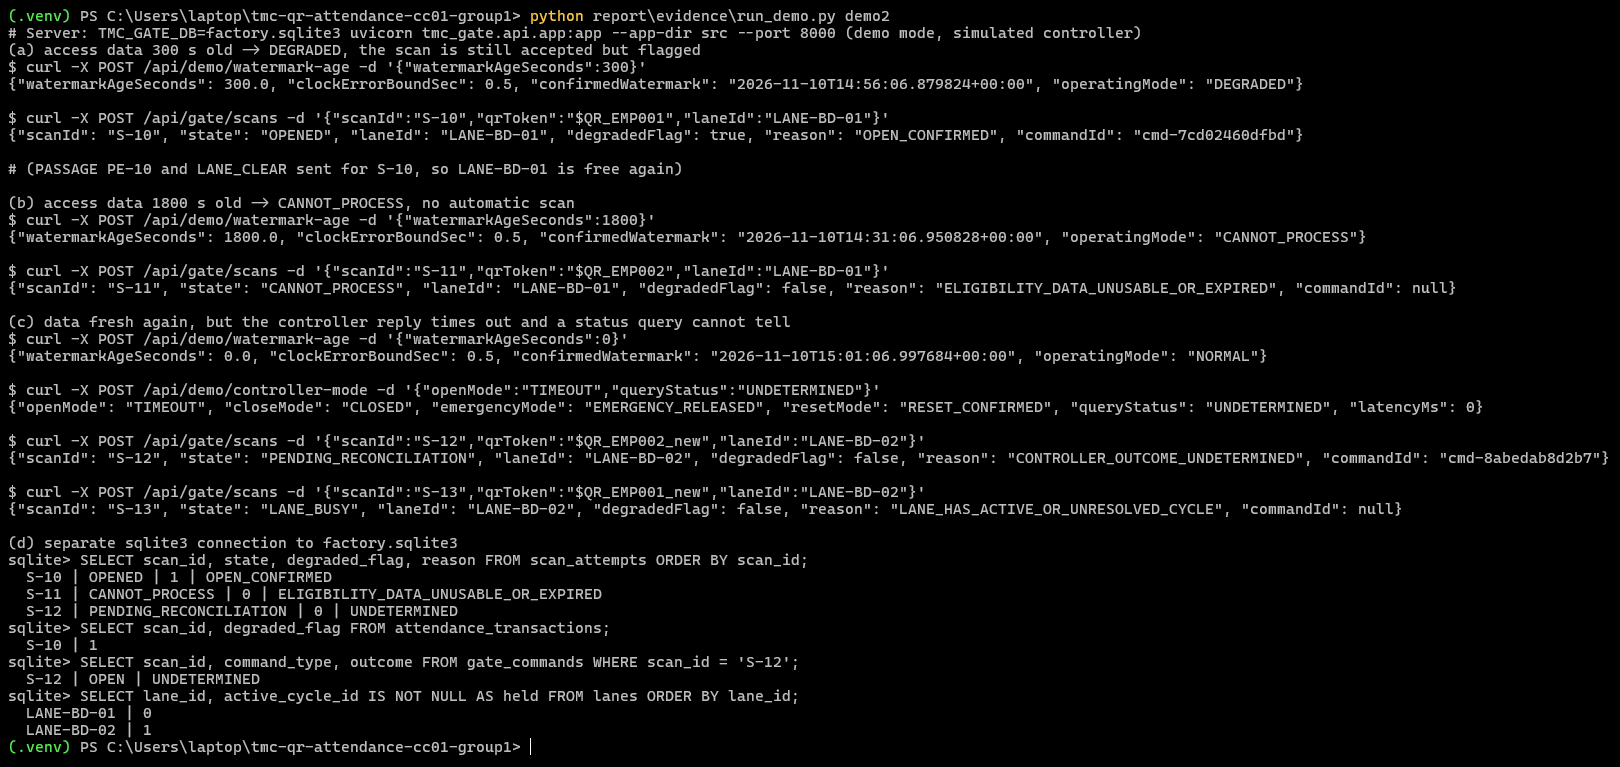
\includegraphics[width=\linewidth]{figure/figure-9-6-degraded-undetermined-run.png}

\vspace{6pt}
\textbf{Figure 9.6. Degraded Mode, CANNOT\_PROCESS, and an Uncertain Opening on Uvicorn}
\phantomsection\addcontentsline{lof}{figure}{\protect\numberline{9.6}Degraded Mode and an Uncertain Opening on Uvicorn}
\end{minipage}

\vspace{10pt}

Figure 9.7 runs the local part of Flow B. An assisted opening without a guard session gets HTTP 401 (a). With the session, the same request sent twice returns the same commandId both times (b). We then played the controller for this assisted opening and sent a PASSAGE right away, well inside the 15-second window, followed by LANE\_CLEAR (c). For a QR scan the same two signals created an attendance record in Figure 9.5. An emergency release puts LANE-BD-01 in EMERGENCY\_HOLD, and a QR scan on that lane gets LANE\_BUSY (d). After the reset and a LANE\_CLEAR the gate is closed and the next scan is OPENED again (e). In the database (f), case-001 has one stored OPEN command and one CLOSE command, the passage PE-30 is stored without a review reason, and there is still no attendance record. So a timely passage through an assisted opening did not create attendance by itself. The run does not show the later HR approval step, which is outside the prototype.

\noindent\begin{minipage}{\linewidth}
\centering
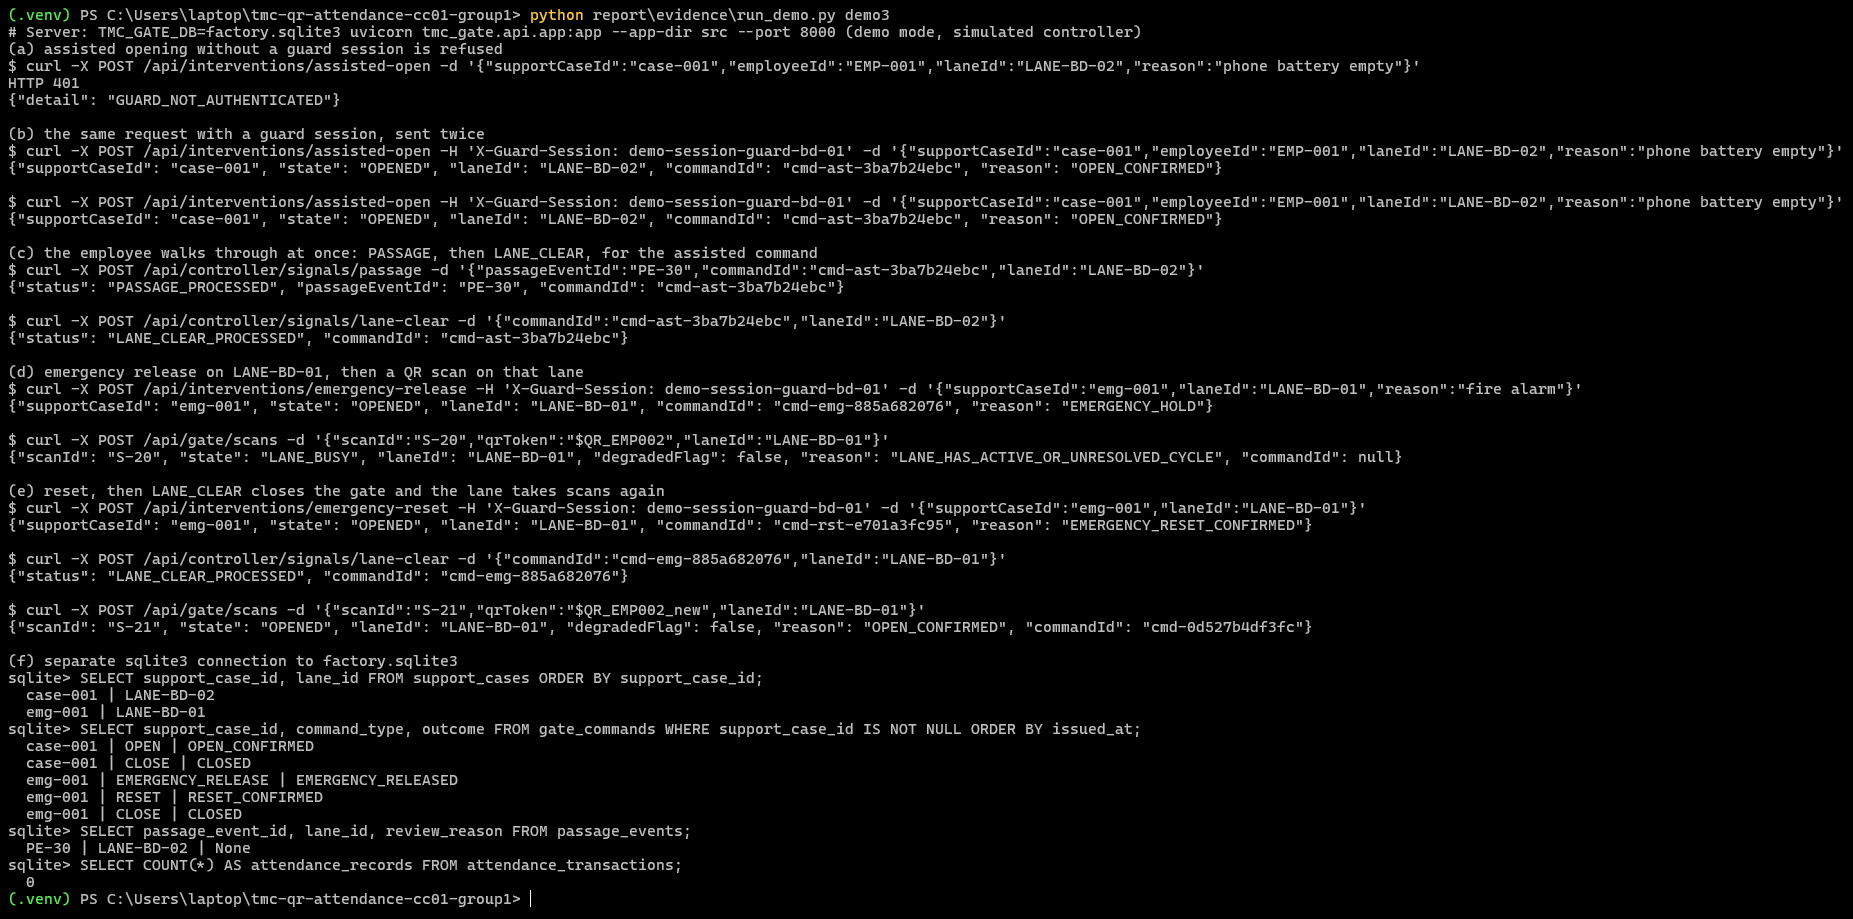
\includegraphics[width=\linewidth]{figure/figure-9-7-flow-b-run.png}

\vspace{6pt}
\textbf{Figure 9.7. Flow B on Uvicorn: Guard Session, Assisted Opening with a Passage, and Emergency Hold}
\phantomsection\addcontentsline{lof}{figure}{\protect\numberline{9.7}Flow B on Uvicorn}
\end{minipage}

\vspace{10pt}

\Needspace{9\baselineskip}
\subsection*{9.6. Design Rules Checked by Tests}

\phantomsection
\addcontentsline{toc}{subsection}{9.6. Design Rules Checked by Tests}

Before the numbers, Table 9.6 links the main gate rules of Chapters 4 to 7 to the tests that check them. Unless the table says otherwise, these tests use in-memory fakes for storage and for the controller, so they check the logic of Gate Core and Gate Intervention rather than the behavior of a real database.

\begin{longtable}{|>{\raggedright\arraybackslash}p{60.5pt}|>{\raggedright\arraybackslash}p{180.5pt}|>{\raggedright\arraybackslash}p{169.5pt}|}
\hline
\multicolumn{1}{|>{\columncolor{tableheader}\centering\arraybackslash}p{60.5pt}|}{\textbf{Source}} & \multicolumn{1}{>{\columncolor{tableheader}\centering\arraybackslash}p{180.5pt}|}{\textbf{Rule}} & \multicolumn{1}{>{\columncolor{tableheader}\centering\arraybackslash}p{169.5pt}|}{\textbf{Test file}} \\
\hline
\endhead
\multicolumn{3}{c}{\rule{0pt}{20pt}\normalsize\textbf{Table 9.6. Design Rules and Their Tests}} \\
\endlastfoot
Flow A, ADR-02 & ACCEPTED, the token claim, and the new GateCycle are stored before openGate; a busy lane returns LANE\_BUSY without claiming the token. & \code{test_pkg3_processor.py}, \code{test_pkg4_sqlite_repos.py}, \code{test_e2e_sqlite_flows.py} \\
\hline
Table 5.5 & openGate gets min(700 ms, time left of the 2-second budget); if no time is left, the scan ends as CANNOT\_PROCESS, the lane is released, and the token stays claimed. & \code{test_pkg3_rules.py}, \code{test_pkg3_pr2_regressions.py} \\
\hline
I-03, Section 7.1.3 & An UNDETERMINED opening is stored, queried once where the port exists, and then moved to PENDING\_RECONCILIATION. The same scan never gets a second open command. & \code{test_pkg3_rules.py}, \code{test_pkg3_pr2_regressions.py}, \code{test_pkg5_adapter_with_processor.py} \\
\hline
I-07, ADR-02 & Attendance is created only after a stored PASSAGE while the scan is still OPENED within 15 seconds; a repeated passageEventId is ignored, a second passage is kept without attendance, and a late passage is stored as LATE\_PASSAGE for review. & \code{test_pkg3_rules.py}, \code{test_pkg3_pr2_regressions.py} \\
\hline
I-05, Table 4.23b & closeGate is sent once after LANE\_CLEAR; the 15-second timer never closes the gate; an old close result cannot release a lane that a new scan holds. & \code{test_pkg3_rules.py}, \code{test_pkg3_pr2_followup.py} \\
\hline
I-10, Section 5.7.2 & NORMAL up to 60 s, DEGRADED below 30 min, CANNOT\_PROCESS from 30 min, or when the clock error bound is unknown or at least 2 s, or the data is not continuous. & \code{test_pkg1_snapshot.py} \\
\hline
ADR-11 & Ed25519 signature, 60-second expiry, factory binding, and single-use claim of tokenId. & \code{test_pkg2_*.py}; two connections claiming one token: \code{test_pkg4_sqlite_repos.py}; copied QR on another lane: \code{test_e2e_sqlite_flows.py} \\
\hline
Flow B, ADR-07 & Assisted opening needs an authorized guard, uses its own 3-second timeout, and creates no attendance; one openGate per supportCaseId, also for two requests at the same time; guardId comes from the session, not the request body. & \code{test_pkg6_intervention.py}, \code{test_pkg6_pr8_*.py}, \code{test_pkg3_rules.py}, \code{test_final_code_edges_regressions.py} \\*
\hline\noalign{\nobreak}
Flow B & Emergency release puts the lane in EMERGENCY\_HOLD and blocks new scans; only RESET\_CONFIRMED for the emergency that holds the lane now ends the hold, so a late reset result for an older emergency returns EMERGENCY\_SUPERSEDED. The RESET command is stored before it is sent. An uncertain result reuses and queries that command; only controller-confirmed non-execution (CONTROLLER\_ERROR) permits a new RESET command. & \code{test_pkg6_intervention.py}, \code{test_pkg3_pr2_regressions.py}, \code{test_final_code_edges_regressions.py} \\
\hline
Flow B & An emergency wins over an open result that arrives after it: a late OPEN\_CONFIRMED creates no attendance, and a late CONTROLLER\_ERROR does not release the held lane. & \code{test_submission_audit_regressions.py}, \code{test_pr15_followup_regressions.py} \\
\hline
Table 4.23b & With no PASSAGE within 15 seconds, the worker moves the cycle to NO\_PASSAGE and the scan to PENDING\_RECONCILIATION, also after LANE\_CLEAR has closed the lane; a PASSAGE committed before the timer wins. & \code{test_submission_audit_regressions.py}, \code{test_pr15_followup_regressions.py} \\
\hline
Section 5.7.2, ADR-05 & Applied access rights survive a restart, a replayed update stays applied, a rolled-back snapshot write is never visible, and a scan does not wait for another request's transaction to read the snapshot. The stored snapshot is read back without type coercion, so a value such as \texttt{"false"} can never turn into an access right. & \code{test_submission_audit_regressions.py}, \code{test_pr15_followup_regressions.py}, \code{test_snapshot_cache_isolation.py}, \code{test_final_code_edges_regressions.py} \\
\hline
\end{longtable}
\phantomsection\addcontentsline{lot}{table}{\protect\numberline{9.6}Design Rules and Their Tests}

The complete Flow B, including HR approval and the resolution feed from the central application, is not tested end to end, because those parts are not in the prototype. The local part of Flow B in the factory application is covered by the end-to-end tests in Section 9.7.

\Needspace{9\baselineskip}
\subsection*{9.7. Test Results}

\phantomsection
\addcontentsline{toc}{subsection}{9.7. Test Results}

Table 9.7 shows the result of \texttt{PYTHONPATH=src pytest} on the submitted version, grouped by work package. We added the last column because a test on fakes and a test on a real SQLite file do not prove the same thing.

\begin{longtable}{|>{\raggedright\arraybackslash}p{112.5pt}|>{\raggedright\arraybackslash}p{134.5pt}|>{\centering\arraybackslash}p{52.5pt}|>{\raggedright\arraybackslash}p{87.5pt}|}
\hline
\multicolumn{1}{|>{\columncolor{tableheader}\centering\arraybackslash}p{112.5pt}|}{\textbf{Test files}} & \multicolumn{1}{>{\columncolor{tableheader}\centering\arraybackslash}p{134.5pt}|}{\textbf{What they cover}} & \multicolumn{1}{>{\columncolor{tableheader}\centering\arraybackslash}p{52.5pt}|}{\textbf{Passed}} & \multicolumn{1}{>{\columncolor{tableheader}\centering\arraybackslash}p{87.5pt}|}{\textbf{Runs against}} \\
\hline
\endhead
\multicolumn{4}{c}{\rule{0pt}{20pt}\normalsize\textbf{Table 9.7. Test Results of the Submitted Version}} \\
\endlastfoot
\code{test_architecture_solid.py} & Import direction of each layer, ISP splits & 4 & Source code \\
\hline
\code{test_pkg1_snapshot.py} & Watermark and clock limits, continuity, local rights & 146 & Domain only \\
\hline
\code{test_pkg2_*.py} & Signature, 60-second expiry, factory binding, key rotation, clock and watermark limits & 26 & Snapshot and real Ed25519 keys \\
\hline
\code{test_pkg3_*.py} & Flow A cycle, deadline, UNDETERMINED, passage and close rules, emergency races & 37 & Fake storage and controller \\
\hline
\code{test_pkg4_*.py} & Atomic write, rollback, concurrent token claim, event deduplication, storage time budget & 50 & SQLite file \\
\hline
\code{test_pkg5_*.py} & One contract on both adapters, processor with real adapters, demo endpoints, review regressions & 135 (+1) & Simulated controller; fake storage or in-memory SQLite \\
\hline
\code{test_pkg6_*.py} & Flow B, guard session, support cases, emergency hold and reset & 27 & Fake storage and controller \\*
\hline\noalign{\nobreak}
\code{test_flow_a_e2e.py} & Flow A over HTTP: scan, status, PASSAGE, LANE\_CLEAR & 1 & Fake storage and controller \\
\hline
\code{test_e2e_sqlite_flows.py} & Flow A (7 tests) and Flow B (3 tests) through \code{create_app()} & 10 & SQLite file, Ed25519, simulated controller \\
\hline
\code{test_submission_audit_regressions.py}, \code{test_pr15_followup_regressions.py}, \code{test_snapshot_cache_isolation.py} & Emergency priority, 15-second timeout worker, snapshot after restart, snapshot cache isolation & 18 & SQLite file through \code{create_app()} \\
\hline
\code{test_final_code_edges_regressions.py} & Reset owned by the current emergency, stored RESET never resent, one openGate per supportCaseId, snapshot read without type coercion & 19 & SQLite file through \code{create_app()} \\*
\hline\noalign{\nobreak}
\multicolumn{2}{|l|}{\textbf{Total} (commit 5bd6721, Python 3.12)} & \textbf{473} & 0 skipped, 1 expected failure \\
\hline
\end{longtable}
\phantomsection\addcontentsline{lot}{table}{\protect\numberline{9.7}Test Results of the Submitted Version}
The ``+1'' in the Package 5 row is the expected failure, and it is there on purpose: it is the adapter that treats a receipt as an opening, and the test shows that it breaks the turnstile contract (Section 9.4). CI on GitHub Actions runs the same suite on every push and pull request, and it was green on this commit. Figure 9.8 is the output of the same suite, run again on the same Windows laptop on the final report commit, where the code is unchanged from 5bd6721. That laptop has Python 3.13, while CI uses Python 3.12, and the result is the same on both.

\noindent\begin{minipage}{\linewidth}
\centering
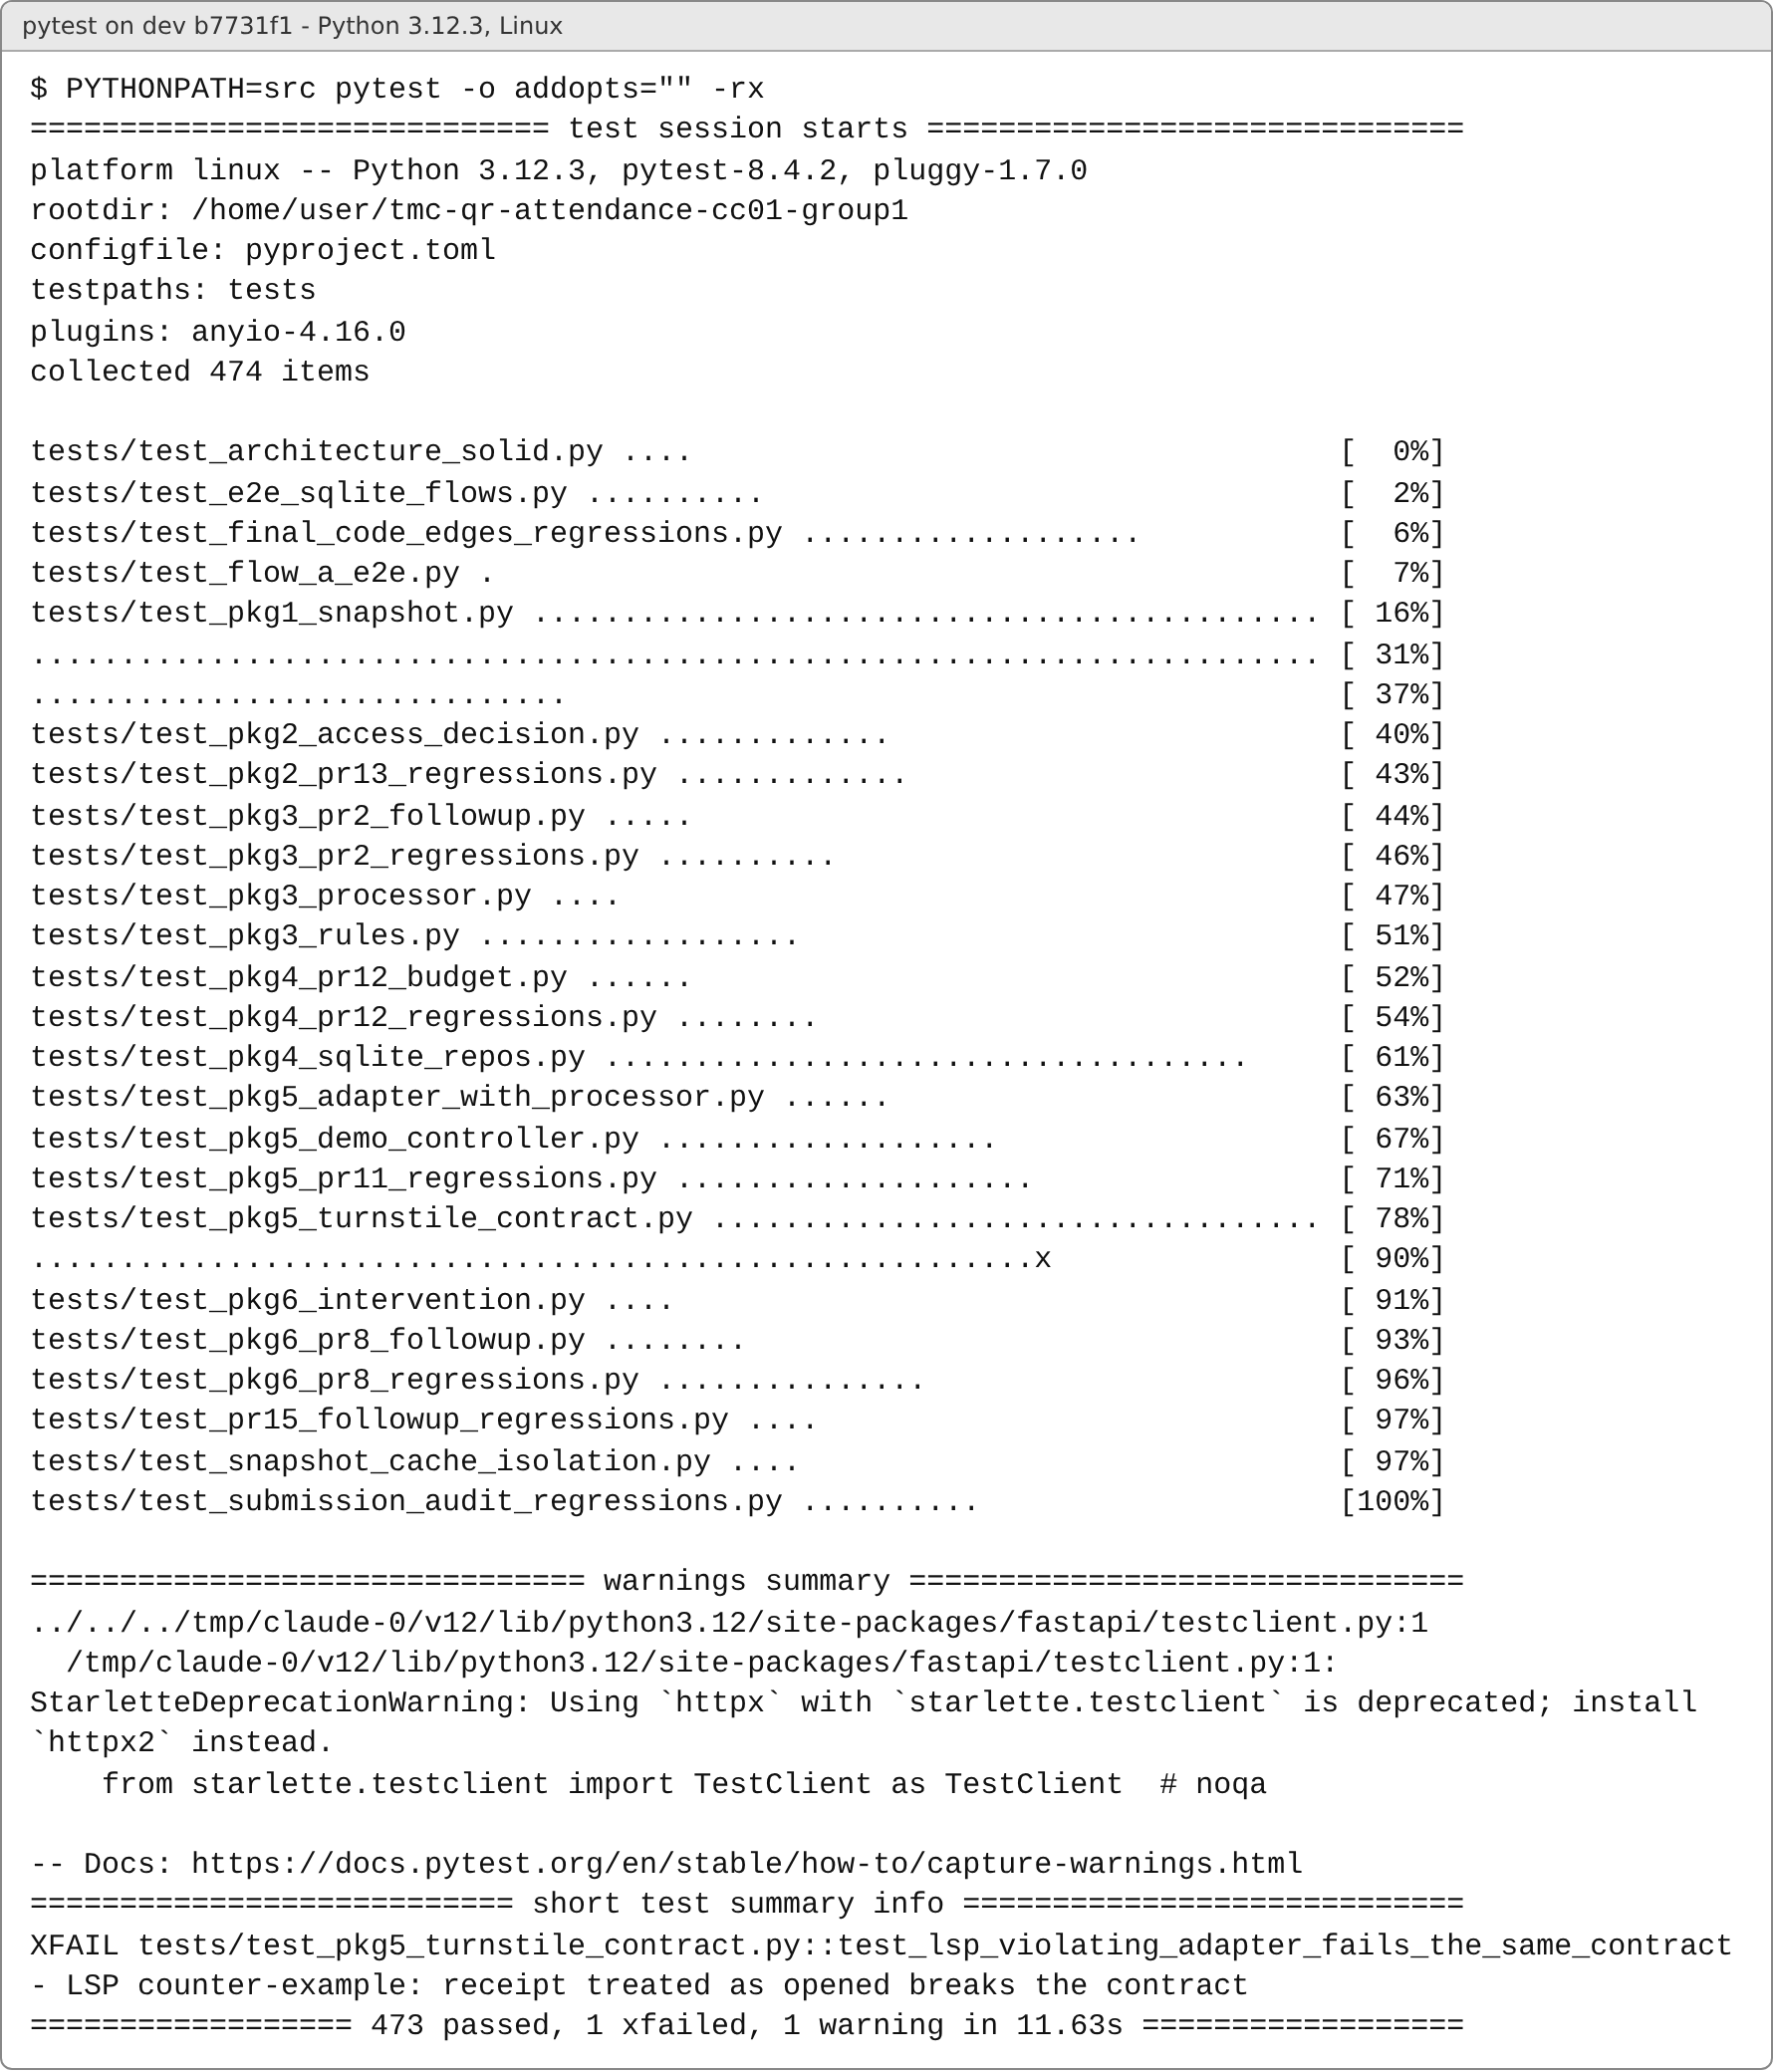
\includegraphics[width=0.92\linewidth]{figure/figure-9-8-pytest-run.png}

\vspace{6pt}
\textbf{Figure 9.8. Output of the Test Suite: 473 Passed and 1 Expected Failure}
\phantomsection\addcontentsline{lof}{figure}{\protect\numberline{9.8}Output of the Test Suite}
\end{minipage}

\vspace{10pt}

The ten tests in \code{test_e2e_sqlite_flows.py} are the closest our automated tests get to a real run. Each one builds the whole application with \code{create_app()} on a real SQLite file, signs QR codes with Ed25519, talks to it over HTTP, and then opens the file with a separate connection to check what was really committed. For Flow A they show that:

\begin{itemize}[leftmargin=36pt, itemsep=2pt, topsep=4pt, parsep=2pt]
  \item a full cycle where the controller sends every signal twice still gives one openGate, one attendance record, and one closeGate;
  \item a copied QR code scanned on another lane is rejected as a replay, and a malformed token or a suspended employee is rejected before any command;
  \item with a watermark age of 300 seconds the scan is accepted in DEGRADED mode and the attendance record carries the degraded flag, and at 1800 seconds the scan is CANNOT\_PROCESS;
  \item an UNDETERMINED opening becomes PENDING\_RECONCILIATION without a second openGate, and the lane and the token stay held; a CONTROLLER\_ERROR releases the lane. The rule that the controller is queried exactly once is checked separately in \code{test_pkg5_adapter_with_processor.py};
  \item the stored state is still there after the application is restarted on the same file.
\end{itemize}

For Flow B they show that a request without a guard session gets HTTP 401, that an assisted opening stores the support case once and creates no attendance, and that an emergency hold makes new scans return LANE\_BUSY until the reset, after which LANE\_CLEAR closes the gate. One rule has no end-to-end test: a PASSAGE that arrives after the 15-second window. It is checked only at processor level (\code{test_pkg3_rules.py}) and for storage (\code{test_pkg4_sqlite_repos.py}).


We also ran the four demo scenarios of the README through FastAPI's TestClient on a SQLite file, and all of them gave the expected results. The three manual runs in Section 9.5 (Figures 9.5 to 9.7) were done on a real Uvicorn server with a SQLite file. Table 9.8 lists what each part of them shows. The order of the writes before openGate and the single closeGate call are checked by the tests in Table 9.6, not by this run. The scripts are kept in \code{report/evidence/}: \code{run_demo.py}, which produced the figures, and bash versions of the same runs together with the captured output and Uvicorn logs of an earlier run, which differ from the figures only in generated ids and times. Clicking through the Swagger page during the presentation is still a manual step.

\begin{longtable}{|>{\raggedright\arraybackslash}p{36pt}|>{\raggedright\arraybackslash}p{124pt}|>{\raggedright\arraybackslash}p{134pt}|>{\raggedright\arraybackslash}p{104pt}|}
\hline
\multicolumn{1}{|>{\columncolor{tableheader}\centering\arraybackslash}p{36pt}|}{\textbf{Figure, part}} & \multicolumn{1}{>{\columncolor{tableheader}\centering\arraybackslash}p{124pt}|}{\textbf{What we sent}} & \multicolumn{1}{>{\columncolor{tableheader}\centering\arraybackslash}p{134pt}|}{\textbf{What we observed}} & \multicolumn{1}{>{\columncolor{tableheader}\centering\arraybackslash}p{104pt}|}{\textbf{What it shows}} \\
\hline
\endhead
\multicolumn{4}{c}{\rule{0pt}{20pt}\normalsize\textbf{Table 9.8. Manual Runs on Uvicorn with a SQLite File}} \\
\endlastfoot
9.5 (a) & Scan S-1 with a fresh QR code on LANE-BD-01 & OPENED, OPEN\_CONFIRMED, and a commandId & Confirmed opening for a valid scan \\
\hline
9.5 (b) & Scan S-2 with the same code on LANE-BD-02 & REJECTED, QR\_TOKEN\_\allowbreak REPLAY\_\allowbreak DETECTED, no command & Single-use token claim (ADR-11) \\
\hline
9.5 (c) & PASSAGE PE-1 twice, then LANE\_CLEAR twice, for the commandId of S-1 & Each request answered with HTTP 200; this alone does not prove deduplication & -- \\*
\hline\noalign{\nobreak}
9.5 (d) & Read the database file with a separate connection & One attendance record (S-1, PE-1, EMP-001, ENTRY), one passage event, one OPEN and one CLOSE command & Repeated signals leave one attendance record and one persisted CLOSE command \\
\hline
9.6 (a) & Watermark age 300 s, then scan S-10 & DEGRADED; S-10 OPENED with the degraded flag; its attendance record is flagged & Bounded degraded mode, flagged for review (I-10) \\
\hline
9.6 (b) & Watermark age 1800 s, then scan S-11 & CANNOT\_PROCESS, no command & No automatic scan from 30 minutes (I-10) \\
\hline
9.6 (c), (d) & openGate times out, status query undetermined; scan S-12, then S-13 on the same lane & S-12 PENDING\_RECONCILIATION with one stored OPEN command, outcome UNDETERMINED; S-13 LANE\_BUSY & Uncertain opening stays pending and keeps the lane held (I-03) \\
\hline
9.7 (a) & Assisted opening without X-Guard-Session & HTTP 401 & Guard comes from the session \\
\hline
9.7 (b) & The same assisted opening twice with a session & Same commandId both times; one stored OPEN command for case-001 & A repeated request reuses the stored command \\
\hline
9.7 (c) & PASSAGE PE-30 at once, then LANE\_CLEAR, for the assisted commandId & HTTP 200 for both; CLOSE command stored for case-001 & -- \\
\hline
9.7 (d), (e) & Emergency release, scan, reset, LANE\_CLEAR, scan & EMERGENCY\_HOLD, LANE\_BUSY, RESET\_CONFIRMED, CLOSED, then OPENED & Emergency hold blocks scans until reset and close \\
\hline
9.7 (f) & Read the database file & Two support cases; PE-30 stored with no review reason; no attendance record & A timely passage after an assisted opening creates no attendance by itself \\
\hline
\end{longtable}
\phantomsection\addcontentsline{lot}{table}{\protect\numberline{9.8}Manual Runs on Uvicorn with a SQLite File}

Table 9.8 only states what can be seen in the HTTP answers and in the database file. A stored command row does not prove how often the adapter was called, and the demo server does not print the command log of the simulated controller. The rule that an uncertain OPEN is not sent again, and that a repeated assisted request does not reach the controller a second time, is therefore checked by tests that count the commands the simulated controller received. In \code{test_e2e_sqlite_flows.py} these are \code{test_flow_a_undetermined_open_is_queried_once_and_never_resent} and \code{test_flow_b_assisted_open_records_case_without_attendance}, and the third is \code{test_resending_identical_support_case_is_idempotent} in \code{test_pkg6_pr8_regressions.py}.

\Needspace{9\baselineskip}
\subsection*{9.8. What the Prototype Does Not Show}

\phantomsection
\addcontentsline{toc}{subsection}{9.8. What the Prototype Does Not Show}

Passing tests do not close the open issues listed in Section 10.2. The simulated controller answers commands the way I-01 and I-03 assume, and the PASSAGE and LANE\_CLEAR signals of I-05 are sent by the tests and scripts, so the runs show that Gate Core handles those signals correctly, but not that a real controller sends them. The tests check how the 2-second budget is shared out using a test clock; they do not measure the response time on factory hardware with a real kiosk and controller. There is also a gap in the budget itself. The prototype starts a 2,000 ms processing budget when processScan begins, because the HTTP route does not pass a kiosk deadline. This budget does not reserve the kiosk, network, and display time allocated in Table 5.4. Meeting NFR-01 requires budgeting those stages together and measuring from QR reading to result display. SQLite has no standby, so the synchronous replication and the failover rules of Section 5.6 are not tested either.

Synchronization is only partly there. IFactoryUpdates applies snapshot changes and reads the local outbox, but without Site Sync or a central application we drive degraded mode by setting the age of the access data by hand. Finally, the guard session and the authorization checks are demo stubs, and the QR private key is created in the same process as the factory code, which the target design does not allow.


\Needspace{9\baselineskip}
\subsection*{9.9. Source Code}

\phantomsection
\addcontentsline{toc}{subsection}{9.9. Source Code}

The implementation, the automated tests, and the LaTeX source of this report are available at

\begin{center}
{\small\url{https://github.com/Khoavan1406-hub/tmc-qr-attendance-cc01-group1}}
\end{center}

The Python package is in \code{src/tmc_gate/}, the tests are in \code{tests/}, and the report source is in \code{report/}. The \code{README.md} file at the root of the repository explains how to install the dependencies, run the test suite, and start the demo, while \code{ARCHITECTURE_RULES.md} records the rules we followed when writing the code, such as the allowed import directions and the gate thresholds. The architectural decisions themselves are not kept as separate files in the repository; they are documented in Chapter 6. All work was merged into the \texttt{dev} branch through pull requests. The code in \code{src/} and \code{tests/} has not changed since commit 5bd6721, which is the commit behind the test results in Section 9.7.


\newpage
% ==================== CHAPTER 10 ====================
\section*{10. CONCLUSION}

\phantomsection
\addcontentsline{toc}{section}{10. CONCLUSION}

This report presents our architecture for TMC's QR-based attendance and access control system at its two factories. It covers the context and requirements, the architecture characteristics, the choice of style, the logical and physical architecture, the main decisions, the design principles, and a prototype of Gate Core and Gate Intervention for Task 2.

\subsection*{10.1. Summary of the Architecture}

\phantomsection
\addcontentsline{toc}{subsection}{10.1. Summary of the Architecture}

\begin{itemize}[leftmargin=36pt, itemsep=2pt, topsep=4pt, parsep=2pt]
  \item \textbf{Characteristics.} The six drivers are reliability and data integrity, availability, performance, security and privacy, auditability, and interoperability. A scan has to be answered within 2 seconds, and accepted records must survive a factory's WAN outage.
  \item \textbf{Style.} Six styles were compared, and we chose Service-based Architecture with Event-driven Integration: a gate application and database at each factory, one central application, and three event feeds between them. Inside, each application is a Modular Monolith.
  \item \textbf{Logical architecture.} Thirteen modules communicate through public interfaces and two ports, and the C\&C View describes three runtime flows. The gate flow keeps four facts apart: the controller received the command, the gate opened, an employee passed, and the gate closed. Only a linked passage creates automatic attendance (I-07), and an uncertain opening is checked or reconciled, never resent.
  \item \textbf{Physical architecture.} Each factory has a primary and a standby server. The central site has a reverse proxy pair, two application instances, a database pair, a broker, monitoring, and backups. The 2-second budget is split over the factory-local path with a 200 ms reserve, and a bounded degraded mode keeps the gates working when the WAN link fails, until the last confirmed watermark is 30 minutes old (I-10).
  \item \textbf{Decisions and principles.} Eleven ADRs record the main choices and their trade-offs. SOLID, cohesion, and coupling keep the module boundaries clear, while short-lived factory-bound QR codes, server-side authorization, audit at the source, and data minimization protect access and personal data.
\end{itemize}

The design gives up the simplicity of a single deployment and accepts that central data lags behind the gates. In return, scans stay on the factory LAN, each factory keeps working when its link fails, and every gate record is stored before it leaves the factory.

\Needspace{9\baselineskip}
\subsection*{10.2. Limitations and Open Issues}

\phantomsection
\addcontentsline{toc}{subsection}{10.2. Limitations and Open Issues}


The prototype in Chapter 9 checks the Gate Core rules on a real SQLite file with a simulated controller, but the design still has to be verified against the real APIs and infrastructure. The main open points are:

\begin{itemize}[leftmargin=36pt, itemsep=2pt, topsep=4pt, parsep=2pt]
  \item \textbf{External contracts.} Command receipt, opening confirmation, passage and lane-clear events, close confirmation, status lookup, and duplicate protection must be verified with the real controller (I-01, I-05), and HR/Payroll receipt semantics must be checked (I-02), including whether an acknowledgement means that the data is ready for reconciliation (IC-01).
  \item \textbf{Gate evidence.} Closing after LANE\_CLEAR with the controller's safety interlock, and counting attendance only after passage, are our assumptions, not capabilities stated in the assignment. If the API has no reliable passage evidence, TMC must add a verified passage sensor before automatic QR attendance is enabled. Until then, cases need documented assistance and HR approval, and OPEN\_CONFIRMED never creates provisional attendance. If safe-closing signals are missing, the closing procedure must be redesigned and tested before operation.
  \item \textbf{Business and display rules.} TMC must confirm whether shifts restrict physical access as well as attendance aggregation (I-06), and whether the QR code must be shown directly in company email rather than through an authenticated link (I-08).
  \item \textbf{Degraded mode.} TMC must approve the 60-second and 30-minute limits (I-10). The longer limit bounds acceptance using old access rights to less than 30 minutes after the last confirmed watermark; it does not guarantee that revocations arrive within that time. At the limit, guards use the manual procedure, which needs a staffing plan. A central issuing outage stops automatic scans sooner, within about 60 seconds as existing QR codes expire. The prototype tests both time limits and the DEGRADED flag for one factory (Chapter 9), but the review cases created after reconnection still need testing with Site Sync and the central site.
  \item \textbf{Anti-replay.} The prototype shows that two concurrent connections cannot claim the same token, but single-use tokens must still be tested under failover and backup restore before disconnected operation is enabled. A code shared live within its 60 seconds is not blocked (Table 5.11), so TMC must decide whether a person check is needed.
  \item \textbf{Operational targets.} The response-time, failover, recovery, and backup targets must be measured with representative loads and failures.
  \item \textbf{Infrastructure.} Synchronous replication makes the standby part of every write. When the synchronous commit cannot be met, new scans that would open a gate stop (Section 5.6.2), and TMC must accept this operational impact. Controller links without TLS need network isolation and restricted access.
  \item \textbf{Data retention.} TMC must confirm retention periods for attendance, support records, audit logs, and backups.
\end{itemize}


\end{document}
